\documentclass[11pt, a4paper, twoside]{custard}
\RequirePackage[l2tabu, orthodox]{nag}
\usepackage{amsmath}
\usepackage{bussproofs}
\usepackage{csp}
\usepackage{fancybox}
\usepackage{hetcasl}

\usepackage{listings}
\lstset{
language=Java,
basicstyle=\small,
numbers=left, numberstyle=\tiny, numbersep=5pt, numberblanklines=false,
linewidth=\linewidth, breaklines=true,
framexleftmargin=5mm, frame=single,
captionpos=b}

\usepackage{tabularx}
\usepackage{tikz}
\usepackage{multicol}
\usepackage{stmaryrd}
\usepackage{placeins}
\usepackage{mathtools}
\usepackage{adjustbox}
\usepackage{framed}
\usepackage{xfrac}
\usepackage{appendix}
\usepackage{geometry}
\usepackage{afterpage}
\usepackage{wrapfig}

\usepackage{graphicx}
\usepackage{caption}
\usepackage{subcaption}
\usepackage{stackengine}
\usepackage{latexsym} 
\usepackage{a4wide}
\usepackage{outlines}

\usepackage{float}

%Bibliography
\usepackage[square,numbers]{natbib}
%\bibliographystyle{plainnat}
\bibliographystyle{abbrvnat}
%\bibliographystyle{dinat}
%\bibliographystyle{plain}
%\bibliographystyle{alpha}

\usepackage{pgfplots}
\pgfplotsset{width=10cm,compat=1.9}
%\usepgfplotslibrary{external}
%\tikzexternalize 

\usepackage{xurl}
%\usepackage[obeyspaces,spaces,hyphens]{url}
\urlstyle{sf}

\usepackage[colorlinks, linkcolor=blue, anchorcolor=blue, citecolor=blue, filecolor=blue, menucolor=blue, runcolor=blue, urlcolor=blue]{hyperref}
%\usepackage[colorlinks, linkcolor=black, anchorcolor=black, citecolor=black, filecolor=black, menucolor=black, runcolor=black, %urlcolor=black]{hyperref}

%% packages required for UML diagrams
\usepackage{tikz-uml} %%package not found
%\usepackage{pgf-umlsd}

%% packages required for simple tree diagrams
\usepackage{tikz-qtree}
\usetikzlibrary{trees}

\newtheorem{myEx}{Example}

\setlength{\arrayrulewidth}{.25 mm}
\renewcommand{\arraystretch}{1.5}

\DeclareMathAlphabet{\mathcm}{T1}{cmr}{m}{it}

%Enumeration number styles
\usepackage{enumitem}
\renewcommand{\labelenumii}{\arabic{enumi}.\arabic{enumii}}
\renewcommand{\labelenumiii}{\arabic{enumi}.\arabic{enumii}.\arabic{enumiii}}
\renewcommand{\labelenumiv}{\arabic{enumi}.\arabic{enumii}.\arabic{enumiii}.\arabic{enumiv}}

%% Include the users customisations.
%% Here you can specify new commands and environments that you intend
%% to use. Using commands can make your document easier to write, read
%% and be more consistent.

%% An example could be
%% \newcommand{\CASL}{\textrm{\textsc{Casl}}\xspace}
%% This would define the command \CASL, that would produce the LaTeX
%% code '\textrm{\textsc{Casl}}' (with an appropriate space at the
%% end) each time it was used.


\newcommand{\CCSig}{\textsc{CspCaslSig}\xspace}
\newcommand{\CCSigN}{\textsc{CspCaslSig}^{plain}\xspace}

\newenvironment{LINES}{\array[t]{@{}l@{}}}{\endarray}


\newcommand{\point}[1]{
    \todo[inline, color=blue!20]{
      $\blacktriangleright$ #1
    }
}

\newcommand{\subpoint}[1]{
    \todo[inline, color=blue!20]{
      $\qquad \vartriangleright$ #1
    }
}

\newcommand{\appendixLemma}[2]{\noindent \textbf{Lemma \ref{#1}} #2}

\newcommand{\XML}{XML\xspace}
\newcommand{\EP}{EP2\xspace}

\newcommand{\ConsExt}{\mathrel{\text{\textit{ConsExt}}}}
\newcommand{\image}{\mathop{\text{\textit{image}}}}

%% WADT 06 paper
\newcommand{\inp}{\mathit{param}}
\newcommand{\comms}{\mathit{comms}}
\newcommand{\denotation}{\mathit{denotation}}

%% General
\newcommand{\CASL}{\textrm{\textsc{Casl}}\xspace}
\newcommand{\CSP}{\textrm{\textsc{Csp}}\xspace}
\newcommand{\CC}{\CSP-\CASL}
\newcommand{\SCC}{Structured \CSP-\CASL}
\newcommand{\CSPProver}{\CSP-Prover\xspace}
\newcommand{\CCProver}{\CC-Prover\xspace}
\newcommand{\Hets}{\textrm{\textsc{Hets}}\xspace}
\newcommand{\SPASS}{SPASS\xspace}
\newcommand{\ML}{ML\xspace}

\newcommand{\Nat}{\mathbb{N}\xspace}

\newcommand{\expandsTo}{\widehat{=}}

%% The def extension on sorts, .e.g., s_def
\newcommand{\sortdef}{\text{\textit{def}}}

\newcommand{\partialInv}[1]{{#1}^{-1}}
\newcommand{\invImg}[1]{{#1}^{-}}

\newcommand{\upCl}[1]{\mathop{\uparrow} #1\xspace}
\newcommand{\downCl}[1]{\mathop{\downarrow} #1\xspace}
\newcommand{\downClSet}[1]{{#1}_{\downarrow}\xspace}
\newcommand{\overloadRelProc}{\sim_{N}}

 %% CC: evaluation according to csp semantics relative to csp domain
\newcommand{\cspSemantics}[2]{\sem{#1}_{#2}\xspace}
 %% CC: evaluation according to casl semantics relative to cc
 %% model, local and global variable valuations.
\newcommand{\ccEvalCaslSem}[4]{\sem{#1}_{#2, #3, #4}\xspace}

%% Related work
\newcommand{\ActOne}{\textrm{\textsc{Act-One}}\xspace}
\newcommand{\CCS}{\textrm{\textsc{Ccs}}\xspace}
\newcommand{\CCSCASL}{\textrm{\textsc{Ccs-Casl}}\xspace}
\newcommand{\CASLCHARTS}{\textrm{\textsc{Casl-Charts}}\xspace}
\newcommand{\COCASL}{\textrm{\textsc{Co-Casl}}\xspace}
\newcommand{\CASLLTL}{\textrm{\textsc{Casl-Ltl}}\xspace}
\newcommand{\Lotos}{\textrm{\textsc{Lotos}}\xspace}
\newcommand{\ELotos}{\textrm{\textsc{ELotos}}\xspace}
\newcommand{\CSPM}{\textrm{\textsc{Csp}}\ensuremath{_{\textrm{M}}}\xspace}
\newcommand{\ACP}{\textrm{\textsc{Acp}}\xspace}
\newcommand{\ASF}{\textrm{\textsc{Asf}}\xspace}
\newcommand{\PSF}{\textrm{\textsc{Psf}}\xspace}
\newcommand{\MUCRL}{\ensuremath{\mu}\textrm{\textsc{Crl}}\xspace}
\newcommand{\MCRL}{\textrm{\textsc{MCrl}}\xspace}
\newcommand{\MUCRLTwo}{\ensuremath{\mu}\textrm{\textsc{Crl2}}\xspace}
\newcommand{\CRL}{\textrm{\textsc{Crl}}\xspace}
\newcommand{\CTLStar}{\ensuremath{\textrm{\textsc{Ctl}}^{*}}\xspace}
\newcommand{\CSPOZ}{\textrm{\textsc{Csp-OZ}}\xspace}
\newcommand{\Circus}{\textrm{\textsc{Circus}}\xspace}
\newcommand{\Eucalyptus}{\textrm{\textsc{Eucalyptus}}\xspace}
\newcommand{\CZT}{\textrm{\textsc{Czt}}\xspace}
\newcommand{\FDR}{\textrm{\textsc{Fdr}}\xspace}
\newcommand{\ProBE}{\textrm{\textsc{ProBE}}\xspace}
\newcommand{\UTP}{\textrm{UTP}\xspace}
\newcommand{\OSI}{\textrm{OSI}\xspace}
\newcommand{\ISO}{\textrm{ISO}\xspace}
\newcommand{\ObjectZ}{\textrm{\textsc{Object-Z}}\xspace}

%% Semantics
\newcommand{\angles}[1]{\langle #1 \rangle}
\newcommand{\concat}{\mathop{{}^{\smallfrown}}}
\newcommand{\T}{\mathcal T}
\newcommand{\F}{\mathcal F}
\newcommand{\N}{\mathcal N}
\newcommand{\R}{\mathcal R}
\newcommand{\D}{\mathcal D}
\newcommand{\failuresdivergences}{Failures/Divergences\xspace}
\newcommand{\stablefailures}{Stable-Failures\xspace}
\newcommand{\stablerevivals}{Stable Revivals\xspace}

\newcommand{\tick}{\cspTick}
\newcommand{\powerset}{\ensuremath{\mathcal P}}
\newcommand{\trBot}{tr_{\bot}}
\newcommand{\restrictedTo}[1]{\upharpoonright #1}
\newcommand{\sem}[1]{\llbracket #1 \rrbracket}
\newcommand{\cspRef}{\sqsubseteq}
\newcommand{\cspRefReversed}{\sqsupseteq}
\newcommand{\ccref}{\leadsto}


\newcommand{\RefCl}{\mathop{\text{\textit{RefCl}}}}

\newcommand{\traces}{\mathop{\text{\textit{traces}}}}
\newcommand{\failures}{\mathop{\text{\textit{failures}}}}
\newcommand{\failuresBot}{\mathop{\text{\textit{failures}}_{\bot}}}
\newcommand{\failuresBotI}{\mathop{\text{\textit{failures}}_{\bot, I}}}
\newcommand{\divergences}{\mathop{\text{\textit{divergences}}}}
\newcommand{\Network}{\mathop{\text{\textit{Network}}}}

\newcommand{\ccalph}{\ensuremath{\mathop{\textit{Alph}}}}
\newcommand{\ccalphReduct}{\ensuremath{\mathop{\textit{Alph\_Reduct}}}}
\newcommand{\alphEmb}[1]{\overline{#1}}
\newcommand{\strip}{\ensuremath{\mathop{\text{\textit{strip}}}}}

\newcommand{\cspTop}{\text{\textit{Top}}}

%% From MPhil
\newcommand{\category}[1]{\ensuremath{\mathop{\text{\textbf{#1}}}}}
\newcommand{\functor}[1]{\ensuremath{\mathop{\text{\textbf{#1}}}}}
\newcommand{\functorsymbol}[1]{#1}

\newcommand{\ModReduct}{\ensuremath{\category{Mod\_Reduct}}\xspace}

% These are institution functors
\newcommand{\Sen}{\functor{sen}}
\newcommand{\ModFunctor}{\functor{mod}}

% these are (projection) functions
\newcommand{\Sig}{\ensuremath{\mathop{\text{\textbf{Sig}}}}}
\newcommand{\Mod}{\ensuremath{\mathop{\text{\textbf{Mod}}}}}
\newcommand{\Axioms}{\ensuremath{\mathop{\text{\textbf{Ax}}}}}
\newcommand{\flatten}{\ensuremath{\mathop{\text{\textit{flatten}}}}}
\newcommand{\LHS}{L.H.S\xspace}
\newcommand{\RHS}{R.H.S\xspace}
\newcommand{\Isabelle}{Isabelle\xspace}
\newcommand{\IsabelleHOL}{Isabelle/HOL\xspace}
\newcommand{\inj}{\mbox{\texttt{inj}}\xspace}
\newcommand{\pr}{\mbox{\texttt{pr}}\xspace}
%% Structuring Abreviations
\newcommand{\spec}[1]{\text{\textsc{#1}}}
\newcommand{\Sand}{\mathrel{\mathbf{and}}}
\newcommand{\Sthen}{\mathrel{\mathbf{then}}}
\newcommand{\Srename}{\mathrel{\mathbf{rename}}}
\newcommand{\Shide}{\mathrel{\mathbf{hide}}}
\newcommand{\Sfree}[2]{\mathop{\mathbf{free}} #1 \mathrel{\mathbf{along}} #2}
\newcommand{\Swith}{\mathrel{\mathbf{with}}}
\newcommand{\FA}{\mathcm{FA}}
\newcommand{\FM}{\mathcm{FM}}

\newcommand{\singleValued}[1]{\mathop{\text{Single-valued}}(#1)}
\newcommand{\procCons}[2]{\mathop{\text{ProcConst}}(#1, #2)}
\newcommand{\isDF}[2]{#1 \, \mathbin{isDFin} \, #2 \xspace}
\newcommand{\resToLiveTickOn}[4]{#1 \mathrel{ResToLive^{\tick}} #2 \mathrel{on} #3 \mathrel{in} #4}

\newcommand{\FOL}{\text{\textit{FOL$^{=}$}}\xspace}
\newcommand{\PFOL}{\text{\textit{PFOL$^{=}$}}\xspace}
\newcommand{\PCFOL}{\text{\textit{PCFOL$^{=}$}}\xspace}
\newcommand{\SubPFOL}{\text{\textit{SubPFOL$^{=}$}}\xspace}
\newcommand{\SubPCFOL}{\text{\textit{SubPCFOL$^{=}$}}\xspace}
\newcommand{\ResSubPCFOL}{\text{\textit{ResSubPCFOL$^{=}$}}\xspace}

\newcommand{\fst}{\mathop{\text{\textit{fst}}}}
\newcommand{\snd}{\mathop{\text{\textit{snd}}}}
\newcommand{\SET}{\category{SET}\xspace}
\newcommand{\SETINJ}{\category{SET\_INJ}\xspace}
\newcommand{\op}{op}
%% The projection of the controlled traces of a csp model
\newcommand{\contTraces}{cTr}

%% Tikz Styles
\tikzstyle{category}     =[circle,draw, minimum size=3cm]
\tikzstyle{categoryLarge}=[ellipse,draw, minimum width=10cm, minimum height=5.5cm]
\tikzstyle{functor}      =[->, above, shorten <=0.2cm, shorten >=0.2cm]
\tikzstyle{object}       =[]
\tikzstyle{morphism}     =[->]


\newenvironment{discussion}
{\begin{Sbox}\begin{minipage}{0.95\textwidth}\textbf{Discussion:}}
{\end{minipage}\end{Sbox}\begin{center}\shadowbox{\TheSbox}\end{center}}


% Haskell listings.
%
% Style for all Haskell code.
%
\lstdefinestyle{haskell}
    {language=Haskell,
      columns=fixed,
      %%columns=fullflexible,
      showstringspaces=false,
      %%numbers=left,
      %%numberstyle=\tiny,
      basicstyle=\small\ttfamily,
      numbersep=5pt,
      %%numberblanklines=false,
      %% breaklines=true,
    }
%
% Environment for long Haskell listings.
%
\lstnewenvironment{HaskellCode}
  {\lstset{style=haskell, frame=single}}
  {}

\newcommand{\inHaskell}[1]{\lstinline[style=haskell]{#1}}

\newcommand{\amalgamate}{\oplus}
\newcommand{\abovearrow}[1]{\overset{\rightarrow}{#1}}

\newcommand{\GRKH}{\text{Grigore Ro\c{s}u and Klaus Havelund}}
\newcommand{\RH}{\text{Ro\c{s}u-Havelund}}
\newcommand{\RRH}{\text{Reverse-Ro\c{s}u-Havelund}}
\newcommand{\Buchi}{\text{B\"{u}chi}}

%LTL symbols
\newcommand{\LTLeventually}{\Diamond}
\newcommand{\LTLnext}{\scalebox{1.4}{$\circ$}}
\newcommand{\LTLalways}{\square}

\newcommand{\LTLonce}{\ensurestackMath{%
  \stackengine{.5pt}{\Diamond}{\scalebox{.6}[1.2]{$-$}}{O}{c}{F}{F}{L}}}

\newcommand{\LTLprevious}{\scalebox{1.4}{\ensurestackMath{%
  \stackengine{.5pt}{\circ}{\scalebox{.4}[.85]{$-$}}{O}{c}{F}{F}{L}}}}

\newcommand{\LTLalwaysbeen}{\ensurestackMath{%
  \stackengine{.5pt}{\square}{\scalebox{.7}[1.2]{$-$}}{O}{c}{F}{F}{L}}}


\usepackage{tikz}
\usetikzlibrary{arrows}
\usetikzlibrary{automata}
\usetikzlibrary{backgrounds}
\usetikzlibrary{calc}
\usetikzlibrary{fit}
\usetikzlibrary{shapes}
\usetikzlibrary{snakes}
\usetikzlibrary{positioning}
\usetikzlibrary{matrix}
\tikzset{sortTZ/.style ={}}
\tikzset{subsortTZ/.style = {draw, <-}}
\tikzset{isomorphicTZ/.style = {subsortTZ, <->}}
\tikzset{fixedTextHeightProblem/.style = {text height=1.5ex,text depth=.25ex}}
\tikzset{every picture/.style={remember picture}}

%\textwidth for tikz pictures
\newsavebox\tikzpicturebox
\newenvironment{resizedtikzpicture}[1]{%
  \def\mywidth{#1}%
  \begin{lrbox}{\tikzpicturebox}%
  \begin{tikzpicture}
}{%
  \end{tikzpicture}%
  \end{lrbox}%
  \resizebox{\mywidth}{!}{\usebox\tikzpicturebox}%
}

%% The custom data for Swansea University and your degree name.
%\title{Detecting Collusion Between Android Processes Using Linear Temporal Logic}
\title{Runtime Verification For Android Security}
\author{Richard Allen}
\awardinginst{Swansea University}
\degree{Master of Research}
\department{Department of Computer Science}
\university{Swansea University}
%\unilogo{graphics/swansea-university-logo}
\unilogo{graphics/1001-SwanUni-Eng 2017 [662] v1}
\date{2022}

%% Memoir defines a variety of styles and can be easily customised to
%% the users preference. Possible values for chapter style include:
%% demo, demo2, demo3, section, hangnum, companion, bianchi,
%% brotherton, chappell, crosshead, culver, dash, madsen. More styles
%% can be found in the memoir manual (currently called
%% memman.pdf). This line can also be commented out so that we don't
%% use a memoir chapter style.
\chapterstyle{bianchi}

\begin{document}

\frontmatter %% Start roman numbering

\maketitle
\declaration

%Abstract
\begin{abstract}

Users of computer systems face a constant threat of cyberattacks by malware designed to cause harm or disruption to services, steal information, or hold the user to ransom.  Cyberattacks are becoming increasingly prevalent on mobile devices like Android.  Attacks become more sophisticated along with countermeasures in an ever-increasing arms race.  A novel attack method is 'collusion', where the attack gets hidden by distributing the steps through many malicious software actors \cite{PrologAppCollusion}.

We investigate the use of runtime verification to detect collusion attacks on the end-users device.  We have developed a novel algorithm called \RRH\ that is a variation of an existing algorithm by Grigore Ro\c{s}u and Klaus Havelund \cite{RosuHavelund}.  Our approach is computationally efficient enough to detect collusion in realtime on the Android device and does not require prior knowledge of malware source code.  Thus, it can detect future malware without modification to the detection system or the software under scrutiny.

%The Android operating system has found many applications in devices, such as phones, tablets, watches and smart TVs.  It is characteristic that the primary use of these devices is not computation, although they include a computing system as an integral component.  Furthermore, communication with other external computing systems is essential for their functionality, i.e., they are open systems by design.  As such, these devices are vulnerable to typical cyberattacks, including information theft, service abuse, or ransomware.  Attacks happen to such extent that the McAfee Q1 2020 threat report opens with the headline ``Mobile Malware Is Playing Hide and Steal''. \cite{McAfeeMobileThreatReport}
%
%Android regulates what an app is allowed or is not allowed to do, with a \emph{static} permission system.  However, this system has known deficiencies.  First, apps tend to request excessive permissions.  Second, users tend to grant permission without fully understanding the implications in terms of risk.  Third, the permissions system is concerned only with limiting the actions of individual apps.  Even when apps are properly restricted, we have evidence \cite{PrologAppCollusion} that two or more apps in the wild can circumvent the system and collude in malicious activities by combining their permissions.  In a nutshell: under Android, the user does not know what data an app collects, what it does with, or even who it shares data with on or off the device.
%
%In this context, we propose to \emph{dynamically} monitor operating system calls on the device and use techniques from runtime verification to alert the Android user if there is a potential security breach.  The user will have the opportunity to react, e.g., by closing or removing the involved apps.\\
%\\
%Our approach has some advantages:
%\begin{itemize}
%\item The user is informed immediately when the device is under attack.
%\item It is independent of the application code.
%\item It is extensible to further security properties.
%\end{itemize}
%
%Bauer et al. \cite{bauer2012runtime} conducted similar research into using runtime verification within the field of security.  We advance by considering attacks where many apps are involved.  Furthermore, we guarantee that our monitor does not deteriorate over time, i.e., becomes slower with more observations.
%
%To illustrate our approach, we use a simple form of information theft through app collusion as our running example \cite{DetectingMaliciousCollusion}: two apps $A$ and $B$ combine their permissions to steal some information.  To this end, app $A$ first reads information, then shares it with app $B$ via Android inter-app communication, app $B$ then sends information off the device.  A typical example for $A$ could be a contact managing app with access to a user's contacts but no internet access.  App $B$ could be a weather app, without access to contacts, but with access to the
%internet for obtaining the weather forecast.
%
%The Android operating system restricts apps to run in a 'sandbox' that requires access to system resources to go through the operating system.  Thus, \emph{conceptually}, information theft through app collusion can be detected by monitoring operation system calls.  For information theft through collusion to happen, the following sequence of calls is necessary: app $A$ makes a query $q$ to some resource protected by Android and then initiates an inter-app communication to $B$ by calling a send method $s$; app $B$ receives information by calling a receive method $r$, then calls some method to publish information $p$.\footnote{Note that a sequence $\langle q, s, r, p \rangle$ of operating system calls describes information theft only if the published data can be `traced back' to the queried data.}  It is possible to express such trace properties in linear temporal logic (LTL).  For instance, the LTL formula: $$ \LTLonce(p \land \LTLonce(r \land \LTLonce(s \land \LTLonce q)))$$ is satisfied if a trace includes the call pattern necessary for information theft through app collusion.  Other relevant security properties can be expressed in LTL, like ``alert whenever an app takes an image from the camera'' or ``the microphone is never activated before a telephone call has been initiated or accepted''.
%
%In the \emph{technical realisation} of our approach, we use the Xposed framework \cite{rovo89} to intercept calls to security-sensitive Android O/S functions.  A monitor app gets installed on the user's device that logs calls and checks if the collusion security property gets fulfilled.
%
%\begin{center}
%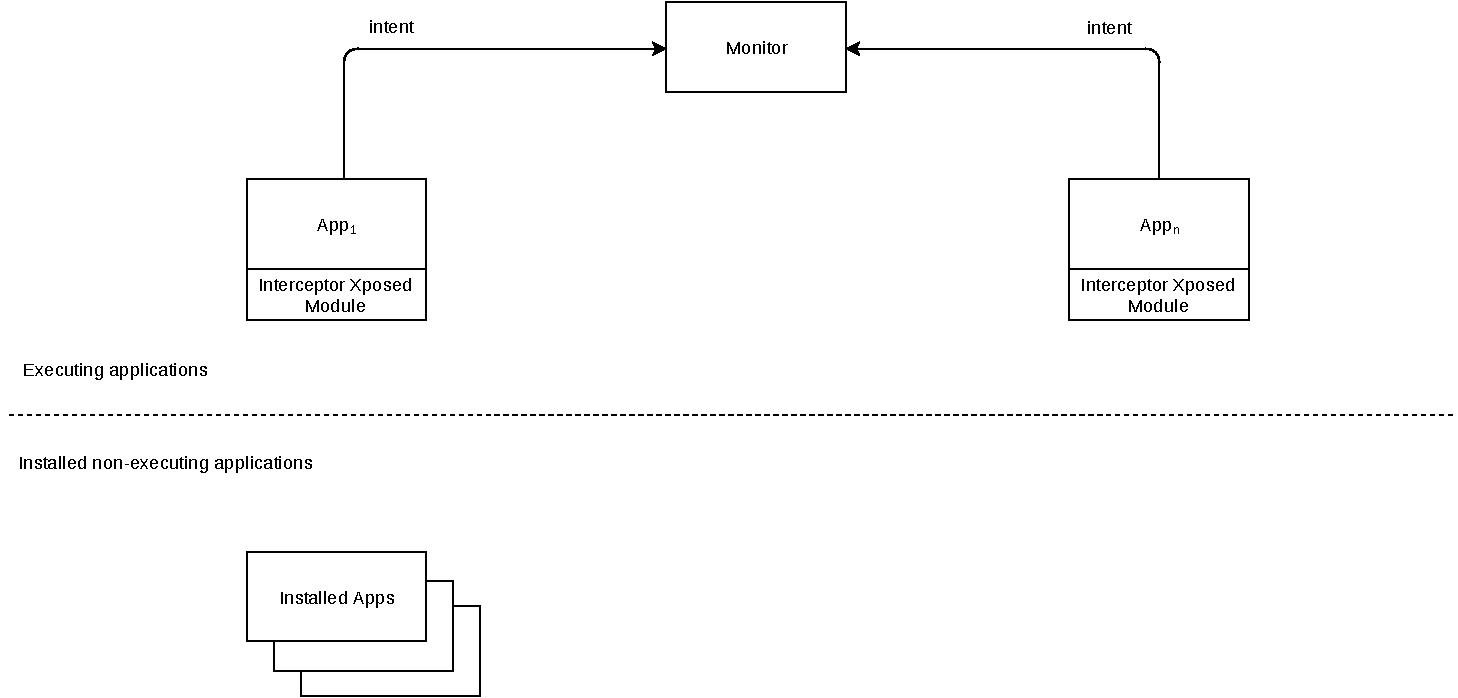
\includegraphics[width=1\textwidth]{graphics/HighLevelArchitecture.pdf}
%\end{center}
%
%For our first attempt to implement a monitor app, we utilised an algorithm by Grigore Ro\c{s}u and Klaus Havelund \cite{RosuHavelund}.  The algorithm appeared interesting thanks to its low complexity: the cost for evaluating a property $\varphi$ on a trace $t$ is $O(|t| * |\varphi|)$, i.e., is linear.  However, the algorithm evaluates a property by traversing the trace from the last event to the first.  This makes it impossible to re-use intermediate results from evaluating $\varphi$ over $t$ for evaluating $\varphi$ over $t {\mathbin{\raise 0.8ex\hbox{$\frown$}}} \langle e \rangle$, i.e., the trace $t$ extended by an event $e$.  In our experiments, this limits the trace length to about 100 events.  Beyond that, the device stopped responding.  Such a trace length is far too short to be of any use in a real-world scenario.
%
%Thus, we created a novel `reverse' version of the algorithm that allows the re-use of intermediate results.  Our new algorithm performs well, i.e., traces can grow to an arbitrary size, and we have tested up to a trace length of 100,000 without encountering any issues.  Evaluation time for new events is in the region of milliseconds for the formula stated above, but this comes at a price: our new algorithm does not support the future LTL operators.
%
%Tests with apps developed for collusion, cf.\ \cite{DetectingMaliciousCollusion}, successfully demonstrated that monitoring is effective on Android hardware without any significant performance reductions.  Evaluation of a new trace event causes CPU usage in the area of 1.5\%.  But to entirely evaluate the performance of our approach, further experimentation into simultaneous monitoring of different security properties will be necessary.  First experiments suggest a linear increase in CPU usage with the total monitored properties.\footnote{Abstract submitted to the CPS-IOT conference for cyber physical systems on the 18th of May 2021 \url{https://sites.google.com/virginia.edu/mt-cps2021/program}}

\end{abstract}


%Acknowledgements
\begin{Acknowledgements}
I first want to thank my primary supervisor Markus Roggenbach for his continuous support in all aspects of the project.
\end{Acknowledgements} 

\newgeometry{top = 4cm}

%Table Of Contents
\tableofcontents*

\restoregeometry

\mainmatter %% Start plain numbering

\chapter{Introduction}

In 2019 it was estimated there were 3.4 billion smartphone users worldwide \cite{SmartphoneUsers2019}.  Smartphones are becoming deeply integrated into our everyday lives.  We use them to navigate, hail taxis, order goods online, and even pay for goods using contactless payment.  Of those 3.4 billion smartphones users, 1.6 billion were using Android devices \cite{AndroidUsers2019}.  But, the use of Android goes beyond just smartphones.  Android is a popular O/S for smart TVs, tablets, automobile infotainment, smartspeakers, smartwatches, and multitudes of other IoT devices.

The threat of malware increases as we adopt these devices.  McAfee has claimed security attacks on Mobile devices are so frequent that in 2020 they opened their threat report with the headline ``Mobile Malware Is Playing Hide and Steal'' \cite{McAfeeMobileThreatReport}.  Android is so prevalent that security gaps and exploitation's can affect large groups of people.  When a person installs an application from an app store, how do they know it is not performing some secret activity?\\
\\
\noindent How can a person be certain that their smartphone is not eavesdropping on conversations?\\
\noindent How can a person be sure the camera on their phone is not surreptitiously sending images to an unknown observer?\\
\\
For the sake of people's privacy and the prevention of crime, the user must always be aware when software is using privacy-sensitive features of their device.

\section{Malware Through Collusion}

Android security prevents applications from accessing sensitive features of the device if it is not permitted by the user.  But, evidence shows that applications can collude to circumvent security permissions \cite{PrologAppCollusion}.  To illustrate collusion, we use a simple form of information theft as our running example \cite{DetectingMaliciousCollusion}: two apps $A$ and $B$ combine their permissions to steal some information.  To this end, app $A$ first reads information, then shares it with app $B$ via Android inter-app communication, app $B$ then sends information off the device.  A typical example for $A$ could be a contact managing app with access to a user's contacts but no internet access.  App $B$ could be a weather app, without access to contacts, but with access to the
internet for obtaining the weather forecast.

The Android operating system restricts apps to run in a 'sandbox' that requires access to system resources to go through the operating system.  Thus, \emph{conceptually}, information theft through app collusion can be detected by monitoring operation system calls.  For information theft through collusion to happen, the following sequence of calls is necessary: app $A$ makes a query $q$ to some resource protected by Android and then initiates an inter-app communication to $B$ by calling a send method $s$; app $B$ receives information by calling a receive method $r$, then calls some method to publish information $p$.  It is possible to express such trace properties in linear temporal logic (LTL).  For instance, the LTL formula: $$ \LTLonce(p \land \LTLonce(r \land \LTLonce(s \land \LTLonce q)))$$ is satisfied if a trace includes the call pattern necessary for information theft through app collusion.

\section{Existing Techniques for Detecting Malware}

Present techniques for detecting malware include machine learning \cite{ThreatAssesmentAppCollusion}, model checking \cite{ModelCheckingCollusion}, and the analysis of Prolog facts extracted from applications regarding their behaviour \cite{PrologAppCollusion}.  Machine learning techniques can estimate the probability that applications are colluding based on their permitted access to sensitive resources and their ability to communicate with each other.   Model-checking is prone to detecting collusion that only exists in the abstract model extracted from source code.  As such, it produces false positives.  Analysing extracted Prolog facts can detect colluding applications, but only within small groups.

All the aforementioned techniques are classified as static analysis and operate at design time.  Publishers like the Google Play store are perfectly positioned to use these techniques to vet applications before the end-user installs them.  But applications and their patches get released at such a prodigious rate that we cannot rely on publishers to do so.

\section{Our Aims}

In this context, we propose to \emph{dynamically} monitor applications after installation by using runtime verification.  The advantages of our approach are:
\begin{itemize}
\item The user is informed immediately when the device is under attack.
\item It is independent of the application code.
\item It is extensible to further security properties.
\end{itemize}

We will produce an Android app that will monitor all other application activity on the device and alert the user if there is a potential security breach.  The user will have the opportunity to react, e.g., by closing or removing the involved apps.

\begin{itemize}
\item It will be possible to install the monitor application on an Android device.
\item The monitor will be capable of detecting security breaches, of the information theft through collusion type, in realtime.
\item The impact of the monitor on the device's performance will be minimal.
\item It will not be necessary to modify the applications involved in a security breach.
\item It is not required for the user to enter security properties themselves.
\item The concrete form of warning the user of a security breach is left open.
\end{itemize}

\section{Performance}

For our first attempt to implement a monitor app, we use an algorithm by Grigore Ro\c{s}u and Klaus Havelund \cite{RosuHavelund}.  The algorithm appears interesting thanks to its low complexity: the cost for evaluating a property $\varphi$ on a trace $t$ is $O(|t| * |\varphi|)$, i.e., is linear.  However, the algorithm evaluates a property by traversing the trace from the last event to the first.  This makes it impossible to re-use intermediate results from evaluating $\varphi$ over $t$ for evaluating $\varphi$ over $t {\mathbin{\raise 0.8ex\hbox{$\frown$}}} \langle e \rangle$, i.e., the trace $t$ extended by an event $e$.  In our experiments, this limits the trace length to about 100 events.  Beyond that, the device stops responding.  Such a trace length is far too short to be of any use in a real-world scenario.

Thus, we introduce a novel `reverse' version of the algorithm that allows the re-use of intermediate results.  Our new algorithm performs well, i.e., traces can grow to an arbitrary size, and we have tested up to a trace length of 100,000 without encountering any issues.  Evaluation time for new events is in the region of milliseconds for the formula stated above, but this comes at a price: our new algorithm does not support the future LTL operators.

Tests with apps developed for collusion, cf.\ \cite{DetectingMaliciousCollusion}, successfully demonstrate that monitoring is effective on Android hardware without any significant performance reductions.  Evaluation of a new trace event causes CPU usage in the area of 1.5\%.

\section{Chapter Overview}

\noindent Starting with Chapter \ref{chap:Collusion} we establish the concept of collusion.  The villain of this story is malware who, in this case, steals information from the Android user.  We refer to prior studies that demonstrate colluding applications can circumvent the security model.\\

\noindent Chapter \ref{chap:Runtime Verification} proposes a software validation technique called Runtime Verification can detect a collusion threat. We first explain the technique and then put its distinguishing features into context with other validation techniques. Then we examine some challenges of using runtime verification to detect collusion.\\

\noindent Linear Temporal Logic goes hand-in-hand with runtime verification and is the subject we introduce in Chapter \ref{chap:Linear Temporal Logic}.  We cover the concept of a trace of events, followed by the grammar, and semantics of LTL.\\

\noindent Chapter \ref{chap:Rosu-Havelund Algorithm} looks at an algorithm developed by \GRKH\ for evaluating an LTL formula over a trace with low computational cost.  We explain the algorithm using examples that walk through the evaluation of a formula over a trace step-by-step.\\

\noindent Chapter \ref{chap:Android Platform} is an overview of the Android platform architecture, the security model, and communication provisions.\\

\noindent Next, we require a means to record the activities of Android apps. Chapter \ref{chap:Xposed Framework} presents a third-party framework called Xposed for this purpose.  We go into what it does, its origins, and how the framework gives us the ability to log operating system calls made by any application running on Android.  In this chapter, we also describe how to set up the development environment we used.\\

\noindent Chapter \ref{chap:Related Work} puts the project into context with other related work.  We discuss other approaches to detecting collusion and other approaches to Android security in general.\\

\noindent Our contribution begins with Chapter \ref{chap:Monitoring For Security Properties} where we introduce a formula for detecting collusion, discuss some the hazards encountered when developing a monitor, strategies for overcoming them and how we might respond to a security breach.\\

\noindent Chapter \ref{chap:Monitoring System Architecture} progresses to outline the software architecture of our monitoring system, why we have taken this structure, and its benefits.  Then we give some advice on development with the Xposed framework based on experiences acquired during this project.\\

\noindent We investigate the suitability of the \RH\ algorithm to realtime monitoring in Chapter \ref{chap:Runtime Verification with the Rosu-Havelund Algorithm}.  We start with a complexity analysis of the algorithm then seek to validate the outcome by performing practical tests on an implementation.  The results lead us to a discussion of the algorithm's scalability and a conclusion about its suitability to this application.\\

\noindent Following our discoveries regarding the \RH\ algorithm, we propose a novel algorithm in Chapter \ref{chap:Reverse Rosu-Havelund Algorithm} that is a variation upon the standard algorithm and name it \RRH.  We compare our new algorithm to the standard, declare a consequence of using our new algorithm and then demonstrate the algorithm in operation by dry running it with an example property.\\

\noindent Implementation of the novel algorithm within a working realtime monitor is covered in Chapter \ref{chap:Implementing The Monitor}.  We describe the design of the monitor, functional and performance testing, and then discuss the scalability improvement that the \RRH\ algorithm brings and it suitability to realtime monitoring.\\

\noindent In the final chapter of the contribution, Chapter \ref{chap:MonitorInAction}, we bring together everything from the design and implementation into a demonstration of our monitor detecting collusion between two applications running on a real Android device.\\

\noindent Chapter \ref{chap:Summary} summarises the project and we pose research questions for further studies in chapter \ref{chap:Future Work}.

\section{Presentation}

On the 18th of May 2021, we presented our work to a workshop conference for cyber-physical systems (2021 CPS-IOT).  The conference was hosted by Vanderbilt University and sponsored by the Association for Computing Machinery, IEEE, NSF, and SIGBED.  An abstract got submitted, peer-reviewed and is on the conference website at \url{https://sites.google.com/virginia.edu/mt-cps2021/program}.  We received positive feedback and some valuable points on our presentation.

\part{Background}
\chapter{Collusion}
\label{chap:Collusion}

In this chapter we consider what is informally called malware, how malware differs from useful software and confront the limitations to detecting malware.  We then introduce collusion as a special type of malware and give a formal description.

\section{Malware on Android}
The term `malware' is a portmanteau of malicious and software.  Malware is software that intentionally performs activities that are detrimental to the user, computer systems or networks.  The intentions are to cause harm, disruption, make a financial gain or steal information.  In short, we can associate this software with unlawful activity.  Malware must hide its real intention from the user and thus, will pose as benign software that offers some attractive service.  But unknown to the user, it will perform other functions that benefit the creator in ways the user has not consented to.\\

Android is one of the two most popular platforms for mobile devices, iOS being the second.  In 2019 it was estimated there were 3.4 billion reported smartphone user's worldwide \cite{SmartphoneUsers2019}, and 1.6 billion were Android smartphones \cite{AndroidUsers2019}.  Malware is not just a theorised problem for Android, it is real, and can potentially affect all Android users.  Just a selection of reports contain hundreds of malware examples discovered in the wild: \cite{GhimobMalware}, \cite{AlienMalware}, \cite{CryloggerInTheWild}.\\%  Attacks happen to such an extent that the McAfee Q1 2020 threat report opens with the headline ``Mobile Malware Is Playing Hide and Steal'' \cite{McAfeeMobileThreatReport}.  The report goes on to describe the discovery of a variety of attacks and the latest techniques the authors are using to hide their malware.
\\
On Android devices, malware can take many forms, including:

\begin{enumerate}
\item Information theft is where malware sends information on the device outside the device without the user's permission.  We class spyware as information theft.
\item Ransomware is where information or services are restricted until the user has met the demands of a malicious actor.
\item Monetary theft is where the activities of an application must be paid for financially by the user, such as an application sending SMS messages without the user's permission or responding to advertisements.
\item Controlling device services such as using the device to mine cryptocurrency without the user's knowledge.
\end{enumerate}

In this project, we focus specifically on information theft but, we see no reason why the techniques proposed here cannot be used to detect other types of malware.

\section{The Difference Between Malicious and Benign Software}

ISO27005 defines a security threat as: ``A potential cause of an incident, that may result in harm of systems and organisations.''

The challenge we face when detecting malicious software is that the actions performed during an attack also have harmless purposes.  For instance, many applications can view photos, and many applications communicate with each other to increase the features they offer.  The difference is one of intent.  Operating system calls used for benign purposes can also be put to use by malicious software to perform an attack.  The difference is that malware intends to benefit a malicious actor at the user's expense and without their knowledge.  But without a detailed specification of what the software intends to do, we cannot decide if the actions it performs are to benefit the user or a malicious actor.

The trouble with the Android case is that detailed specifications of applications do not exist. The official publisher of Android applications is the Google Play store.  The descriptions this repository provides are only brief and written by the developer.  Firstly, a malicious developer will not document their real intent, and secondly, the benign developer does not wish to bore the potential user with a technical specification.  For instance, the description of the AccuWeather app begins:\\

``From weather updates to today's temperature, get the accurate weather forecast you know you can rely on with AccuWeather. With in-depth forecast news, the latest forecast updates, severe weather alerts, today's weather, and much more. Our precision and scientific accuracy let you stay one step ahead of the daily forecast and is the weather tracker that makes the unpredictable, predictable.''\\

The description continues in this vein but says nothing about the user's privacy. The Play store does attempt to help the user further by providing reviews from other users. However, user reviews cannot be trusted because we know from the 2020 McAfee threat report \cite{McAfeeMobileThreatReport} that malware already exists with the ability to post fake reviews for other malware.

Without a documented objective, how can we tell if the actions performed are to achieve that objective or a hidden malicious objective?  We cannot tell.  We can only recognise behaviour patterns that suggest applications may be behaving in a threatening manner.  Once we identify a threat pattern, we have no other option but to make the pessimistic assumption that the applications are involved in malicious activity.  Then, at the very least, we can alert the user to decide what to do next.  In the absence of knowledge of intent, any technical process employed to detect malicious activity must work on this assumption.

\section{Collusion as a Special Form of Malware}

Despite the difficulty detecting malware, there is progress.  Efforts to combat malware are effective enough to force malicious actors to greater lengths to disguise a security attack.  We predict the next tactic in the cybersecurity arms race is to hide an attack by distributing the steps between many different malware apps.  The task of identifying malware becomes harder because each individual app appears to be benign.  In isolation, they do not pose a security risk, and together they may first appear to be collaborating to provide increased services to the user.  But, those individual parts can combine their abilities to perform a coordinated attack.  Each application will execute a specific action from an attack sequence.  The essence of collusion is that the result of applications cooperating achieves a malicious objective that they would be unable to achieve alone.  The Android security model guards against most attacks but cannot recognise collusion as a novel type of malware.  As such, colluding applications can circumvent Android security.

\begin{myEx}

An example of collusion is illustrated in figure \ref{fig:collusionExample}.\\

\begin{figure}[h!]
  \centering
  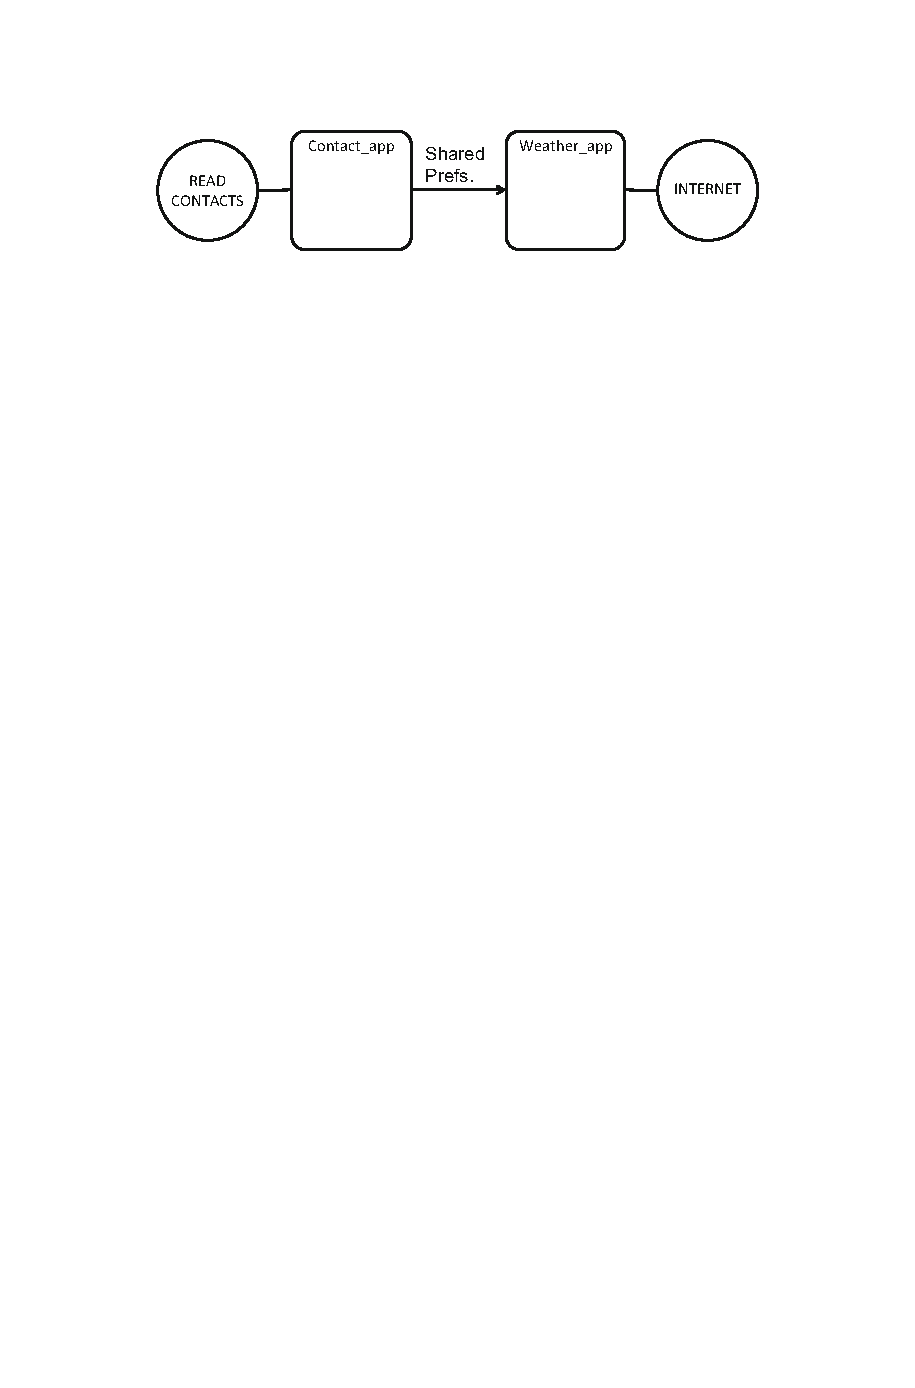
\includegraphics[width=\textwidth]{graphics/CollusionExample}
  \caption{Collusion}
  \label{fig:collusionExample}
\end{figure}

Here two applications are colluding to steal the user's contacts list.  One application has been granted permission to read the contacts list on the user's device but cannot transmit anything off the device.  It can, however, communicate with a second application by writing to a shared preferences file.  The second application has access to the internet for receiving weather updates from an internet server.  These applications are able to combine their permissions to defeat the Android security system and steal information.  The contacts app can read the contact list and pass it to the weather app via the shared file, then the weather app can transmit this information off the device to a hidden actor.

\qed
\end{myEx}

\noindent
A general description of collusion was put forward by As{\u a}voae et al. \cite{DetectingMaliciousCollusion}:\\

\begin{definition}
\label{def:Collusion}
There is a non-singleton set S of apps performing a threat such that:

\begin{itemize}

\item Each app in S contributes the execution of at least one action of the threat.
\item Each app in S communicates with at least one other app in S. 

\end{itemize}
\end{definition}

\noindent
The possibility of collusion was introduced as theoretical concept in 2011 by Schlegel et al. \cite{Soundcomber} where they developed a proof-of-concept called `Soundcomber'.  Soundcomber comprised of two applications communicating to steal the user's banking details.   Then, in 2017, collusion was confirmed in the wild thanks to the ACiD project \cite{ACiDProject}.

\subsection{Staging a Controlled Attack}
\label{sebsec:PerformingAControlledAttack}

In order to develop a means to detect collusion, we must have the ability to perform an attack at will and demonstrate that our countermeasures are able to recognise the attack.  The example in Figure \ref{fig:collusionExample} provides us with the activities that constitute a threat to steal a users contacts list:

\begin{enumerate}
\item Application A reads the contacts list
\item Application A sends the contact list to application B.
\item Application B receives the contact list from application A.
\item Application B publishes the contact list
\end{enumerate}

We can see that applications A and B are attacking the system in a way that follows Definition \ref{def:Collusion} of collusion:  Two applications are involved, each application performs two actions from the threat, and each application is involved in communication with another.  Using that example to provide a collusion stimulus, we will produce two applications that carry out the attack described.  Details of the applications are left to section \ref{subsec:RHPracticalPerformanceAnalysisEnvironment} in the contribution, where we build a test environment.

%The Android security model guards against most attacks but cannot recognise collusion as a novel type of malware.  As such, colluding applications circumvent Android security.

%We demonstrate that colluding applications circumvent the security model.

%We examine how the Android security model guards against most attacks, but can be circumvented by colluding applications.\\

\chapter{Runtime Verification}
\label{chap:Runtime Verification}

In this chapter, we introduce a software validation technique known as runtime verification and explain how it is used to detect software defects.  We examine the unique characteristics that make it valuable among other validation techniques and the associated computational cost.  Then we consider the needs of an Android security system and how we can adapt runtime verification to detecting security breaches instead of software defects.

\section{The Problem of Defects}

Runtime verification is one of many responses to the problem of defects.  A defect is an unwanted system behaviour that falls outside the specification.  Due to their ubiquity, software defects are overlooked by society when they result in nothing more serious than delays and frustrations.  We accept a failure as mere inconvenience when the result is a delayed train, an out-of-order cash machine, or the need to repeat an entry into a website.  But, the problem of defects become more serious when system failures are costly, deadly, or invasive, and automatic control systems find their way into virtually every aspect of our daily lives.

By the late 1960s, the cost of developing software had become greater than the cost to develop hardware.  The phenomenon was named `the software crisis'.  Nowadays, people speak about `the software quality crisis' being where the cost of verifying the correctness of software is greater than the cost of writing software.  In the field of software quality assurance, cost-effective validation techniques are in high demand.

Measuring the defect rate is essential if we are to find effective solutions.  The cause of a defect may be rooted in any of the development stages, but once development has reached the implementation stage, it becomes possible to use the KLOC metric.  KLOC measures the number of defects a developer introduces per thousand lines of delivered code.  When Steve McConnell studied this topic for his book, Code Complete, he arrived at an average defect rate across the software development industry of between 1 and 25 defects per 1000 lines of delivered code \cite{CodeCompleteKLOC}.  The author of this paper can say from 20 years of personal experience in the software development industry that Code Complete is a widely read, well-regarded book, and the figure measured by McConnell is broadly accepted.  More recent measures of faults per line of code show the problem has not improved \cite{BattleOfTheBugs} \cite{Coralogix} \cite{sogetilabs}.


\section{Countermeasures}

It is no surprise to us that defects have, and still do, plague software development.  But with a measure of defect rate, we can grade the efficacy of different approaches to solving the defect problem.  Some of those approaches are:

\begin{enumerate}
\item Software testing.
\item Peer review in the form of code walk-throughs and inspections.
\item The application of measurable coding standards to reduce complexity metrics such as McCabes cyclomatic complexity \cite{CodeCompleteMcCabe}.
\end{enumerate}

\noindent None of these methods can guarantee that all faults will be discovered relative to a given specification.\\

\subsection{Testing}
\label{subSec:Testing}

The most common validation method is testing.  Being a dynamic analysis technique, testing is performed on a system while it is running.  Tests can be generated automatically from a specification but are more commonly generated manually during the development cycle.  To ensure their integrity, independent quality assurance teams must generate and administer tests rather than the software developers.  There are several subcategories: black box, white box, and unit testing; each has its own characteristics.  When black box testing, the QA team has no visibility of the source code; they only use the specification to direct the tests they run.  In the case of white box testing, the QA team can inspect the source code before deciding upon which tests to perform.  Unit testing automates the execution of tests by the test itself being a program that accepts a fragment of the source code as a parameter, otherwise, execution of tests is also manual.  When tests are administered manually the code under test does not require modification but, when executing tests automatically by unit testing, additional development effort is required to produce unit tests.  It may also be necessary to produce mock implementations of subroutines that are required during the test but are not the subject of the test.  And the design of the code under test can also be impacted because it must be possible to substitute subroutines for mocks.  Producing unit tests requires significant development expertise.  The integrity of unit testing is compromised if developers also develop the tests because the QA team lacks the expertise.

But the Achilles heel of testing is common to all categories.  That is, for testing to be complete, a test is required for every possible input to the system.  This means a test for each functional requirement and every possible failure mode.  Regardless of whether testing is manual or automated, testers often assume a testing hypothesis as follows: Provided a system passes finite test cases, then the system is correct for all inputs.  This hypothesis is often not proven but just casually assumed.  Generally, the number of failure modes is too large to cover, or infinite, and therefore it is impossible to test all inputs to the system.  Thus safety and security cannot be guaranteed.  When white box testing, the QA team can use knowledge of the code to judge which inputs it is sensitive to and filter out the rest.  But this can only lessen the coverage problem.

\subsection{Peer Reviews}
\label{subSec:PeerReviews}

Peer reviews are essentially an informal version of static code analysis, they are shown to improve code quality \cite{CodeCompleteCodeReviews} but, the scope and intensity of the analysis are left to the reviewer and so cannot be guaranteed to be complete.\\

%\subsection{Measurable Coding Standards}
%\label{subSec:MeasurableCodingStandards}

\noindent Next, there are formal static analysis methods like code validation using software model checking or code proving tools.  These techniques have their own advantages and limitations:

\subsection{Model Checking}
\label{subSec:ModelChecking}

Software model checking extracts an abstract model of a piece of software from the source code.  The model covers every possible state following the execution of each instruction.  Correctness properties are formulated manually to express a specification, then automated model proving techniques ensure that all possible executions of the code satisfy those properties.  Model checking has a valuable advantage in that the complete behaviour, including all requirements and failure modes, of a system can be examined because the model covers all inputs to the system.  Developers can perform model checking without compromising the integrity of the result because construction and analysis of the model are automated by trusted processes.  NASA successfully used model checking to verify Java bytecode in the 2005 Java Pathfinder \cite{JavaPathfinder} project.  But they concur that it is infeasible for all but the smallest systems of between 10 and 100 KLOC.  The reason being that Model checking suffers from the state explosion problem, meaning there are too many possible states to cover, and the task of analysing all possible executions becomes colossal when dealing with larger systems.

\subsection{Program Provers}
\label{subSec:ProgramProvers}

Validation using code provers such as Microsoft Dafny\footnote{\url{https://www.microsoft.com/en-us/research/project/dafny-a-language-and-program-verifier-for-functional-correctness/}}, KeY\footnote{\url{https://www.key-project.org/}}, or Spark ADA\footnote{\url{https://www.adacore.com/about-spark}}, entails the developer manually augments the source code with a formal specification and derives proofs regarding the correct functioning of the software.  The technique operates on the source code, and while third-parties can disassemble and decompile source code, the compilation process often discards symbols and may intentionally obfuscate the code.  The decompilation process will be unable to reconstruct the original code verbatim.  Without a specification and obfuscated code, the problem presented to the third-party developer becomes akin to reverse engineering.  For this reason, it is a technique best suited to use by the original developer during the development stage.

Being a static analysis technique means code provers benefit from validation of all inputs to the system.  But, in practice, the augmentations can exceed the code.  Development effort to reach proof is high and, to limit cost, it is common for only a select few requirements to be proven.\\

\noindent Table \ref{table:VerificationTechniquesSummarised} summaries the comparison of different verification technique with regard to relevant attributes.

\begin{table}[h!]
%\centering
%\setlength{\arrayrulewidth}{0.5mm}
\resizebox{\columnwidth}{!}{%
%\begin{tabular}{| p{0.18\linewidth} || p{0.135\linewidth} | p{0.135\linewidth} | p{0.135\linewidth} | p{0.15\linewidth} | p{0.15\linewidth} | p{0.21\linewidth} |}
\begin{tabular}{p{0.18\linewidth} p{0.135\linewidth} p{0.135\linewidth} p{0.135\linewidth} p{0.15\linewidth} p{0.15\linewidth} p{0.21\linewidth}}
\hline
& Black Box Testing & White Box Testing & Unit Testing & Model\hspace{0.2\linewidth} Checking & Program Provers & Runtime\hspace{0.4\linewidth}Verification\\
%\hline
\hline
Additional Code Required & No & No & Yes & No & Yes & Monitor required  \\ %\hline
Source Required & No & Yes & Yes & Yes & Yes & Only if logging is not automatic \\ %\hline
Complete\hspace{0.2\linewidth}Coverage & No & No & No & Yes & Complete for selected requirements & No \\ %\hline
Degree of\hspace{0.3\linewidth}Requirement Coverage & Each\hspace{0.6\linewidth}requirement\hspace{0.3\linewidth}needs a test &  Each\hspace{0.6\linewidth}requirement\hspace{0.3\linewidth}needs a test  &  Each\hspace{0.6\linewidth}requirement\hspace{0.3\linewidth}needs a test  & All\hspace{0.6\linewidth}requirements covered & Select\hspace{0.6\linewidth}requirements covered & Select\hspace{0.6\linewidth}requirements covered \\ %\hline
Performed By & Independent QA & QA & QA & Developer & Developer & Independent QA \\ %\hline
Performed\hspace{0.2\linewidth}During & Development cycle & Development cycle & Development cycle & Development cycle & Development cycle & Runtime \\ %\hline
Degree of\hspace{0.3\linewidth}Automation & Automated generation from a specification is possible & Automated generation of inputs & Manual test generation.  Automated test execution & Manual property expression.  Automated model generation, and model checking & Manual proof construction.  Automated evaluation. & Manual logging, property expression, and intervention.  Automated monitor generation, and property evaluation\\ \hline
\end{tabular}%
}
\caption{Attributes of Verification Techniques Summarised}
\label{table:VerificationTechniquesSummarised}
\end{table}

\section{Runtime Verification as an Alternative}

% traces are finite in size - an infinite number of finite prefixes of an infinite trace rather than a finite (single) infinite trace.  Consider a finite trace as an incrementally observed finite prefix of an unknown infinite trace.
% considers only a subset of total possible executions - similar in that regard to testing
% avoids state explosion problem of model checking but can suffer if monitors are Buchi automata based FSM.
% offline or realtime monitoring possible.

Runtime verification occupies a unique position among verification techniques, shown in figure \ref{fig:VerificationTechniqueTree} below.  It is a dynamic analysis technique, in other words, it operates on software while it is running instead of on the source code.  A software entity called a monitor is generated that acts as a watchdog for the system to be verified.  The monitor will raise an alert if a correctness property $\varphi$ is violated.  Correctness properties are formulated to express the safe or secure running of the system.  A property will either specify a correct execution that must be maintained or specify a failure mode that should be prevented.  For example, if the system to be verified is a motorcar, then the seatbelts must be engaged when the vehicle is in motion.  A correctness property would express this rule.  The monitor observes the system and evaluates whether the observed execution satisfies the property.  If not, the monitor can raise an alert or intervene.

\begin{figure}[h!]
	\resizebox{\columnwidth}{!}{%
	\begin{tikzpicture}
	\tikzset{level distance=75pt}
	\Tree [.{Verification}
	        [.{Static Analysis}
	            [.{Informal}
	            	[.{Peer Review} ]
				]
	            [.{Formal}
	            	[.{Model Checking} ]
	            	[.{Program Provers} ]
	            	[.{Code Metrics} ]
				]
	        ] 
			[.{Dynamic Analysis}
				[.{Code Required}
					[.{Manual Execution}
						[.{White Box Testing} ]
					]
					[.{Automatic Execution}
						[.{Unit Testing} ]
					]
				]
				[.{Code Not Required}
					[.{Manual Execution}
						[.{Black Box Testing} ]
					]
					[.{Automatic Execution}
						[.\node[draw]{Runtime Verification}; ]
					]
				]
			]
		]
	\end{tikzpicture}%
	}
	\caption{Runtime Verification Among Other Verification Methods}
	\label{fig:VerificationTechniqueTree}
\end{figure}

Observation of the system requires visibility of either the state of the system or the events leading to state changes.  To achieve this, the system to be monitored must log events or states into a trace.  For brevity, we will describe log entries as events.  The monitor then evaluates whether the trace satisfies the property.  Offline monitoring evaluates a trace after execution has finished and the trace has been captured.  Realtime monitoring evaluates a property over a trace during execution.

%We will use Linear Temporal Logic \cite{Pnueli} to express properties therefore we must use a variety of LTL that operates on finite traces.  We go into detail on LTL in chapter \ref{chap:Linear Temporal Logic}.

When the monitor evaluates a property over a trace, the trace is always finite in length.  When monitoring offline, we are not concerned because execution finished before evaluation, so no more events will ever occur.  Thus the captured finite trace is complete.  But realtime monitoring can continue indefinitely, and therefore the trace can grow to infinite length.   This disparity must get resolved.  With regard to realtime monitoring, traces are considered to be finite but of continuously increasing length.  After each new event, there is a new trace from the concatenation of the previous trace and the new event.  Thus, when monitoring in realtime, there are infinitely many finite traces, where each is the prefix of a single infinite trace.

In either case, the monitor operates only on observed executions rather an operating on all possible executions.  The state explosion problem that model checking suffers from is avoided but, like other dynamic analysis techniques, runtime verification is incomplete.

A valuable feature of runtime verification is that it can be mostly automated because correctness properties do not have to be formulated by the original developer and, monitors are typically \textit{generated} from correctness properties.  The generation process is assumed to be correct, therefore it will produce a correct monitor.  While the applications to be monitored are assumed to be less reliable because we can say nothing about their construction other than it is recognised that all software contains mistakes, therefore we assume they are not correct.

Another valuable feature is that this can all be achieved without access to the source code so long as the system logs its activity.  Thus, runtime verification enables existing software to be verified by entirely independent parties.\\

\noindent Runtime verification offers a lightweight approach to verification that is akin to black box testing but the automation aspect makes it more cost-effective.

\subsection{Monitor Construction}

Properties to be monitored are often expressed as finite state machines, regular expressions or linear temporal logic formulae.  For a given property, monitors can be constructed as finite state machines from \Buchi\ automata.  Figure \ref{fig:FSMConstruction} below shows the steps involved when constructing a monitor in this way.

\begin{figure}[h!]
  \centering
  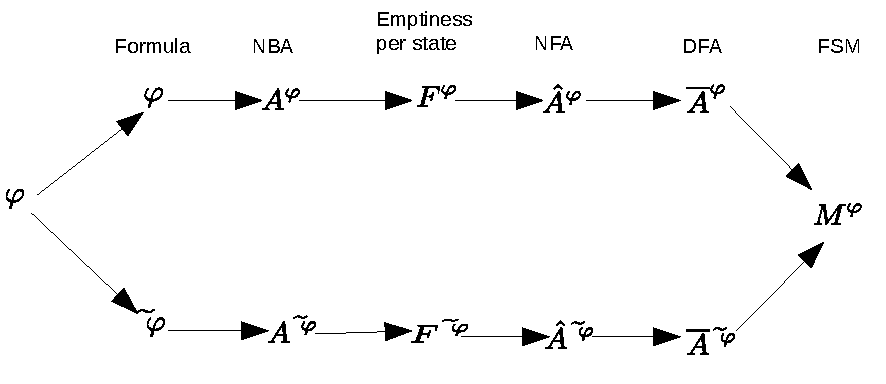
\includegraphics[width=\textwidth]{graphics/BuchiContructionFlow}
  \caption{FSM Based Monitor Construction For a Given Property $\varphi$\cite{RVForLTLAndTLTL}}
  \label{fig:FSMConstruction}
\end{figure}

Two non-deterministic \Buchi\ automata (NBA) are generated from a property supplied as an LTL formula.  One NBA is constructed from the property and the second from its complement.  Emptiness checking is then performed for each NBA by a function that returns $\top$ if the language of the automaton for a given starting state is non-empty.  Using those functions non-deterministic finite automata (NFA) are defined followed by deterministic automata (DFA) for both the property and the complement.  These are combined to yield the final finite state machine.

\subsection{Monitor Complexity}

Complexity is a problem for monitors constructed in this manner.  The second step of construction where NBA get generated is subject to the problem of exponential state blow-up.  The fifth step, which generates deterministic finite automata, also suffers from exponential blow-up.  In the worst case, these two steps lead to the size of the final FSM being $O(2^{2^n})$ \cite{RVForLTLAndTLTL}, thus in the worst case it is too complex.  In practice, however, many monitors generated in this way have lower complexity than the worst case and are useful.  We aim to avoid the exponential blow-up problem entirely by using an alternative technique to generate the monitor.

Regardless of how the monitor is generated, there is always a performance penalty to using runtime verification.  At the very least the system will run slower when it is being monitored because it must log it's activities.  This could be the only performance cost if evaluation of the property happens after execution has finished.  Likewise, it is not essential that the monitor runs on the system being monitored.  But, if monitoring is performed in realtime and on the system being monitored, then the computational cost of running the monitor pushes the performance penalty higher still.  Estimates are that runtime verification can slow a system to half its normal speed.% \cite{RVPermormancePenality}.

\section{Application of Runtime Verification to Security}

We categorise a security breach as a failure mode of the system.  The properties we formulate will get satisfied when a security breach occurs and get violated under correct operation.  We aim to recognise security breaches as they happen and ideally before they are complete.  If a property describes the events immediately before a security breach then, the monitor can raise an alert so that preventative measures can stop the imminent security breach from ever occurring.  To achieve this, we must evaluate properties in realtime and on the Android system.  There is great emphasis on a computationally efficient algorithm.

Due to the aforementioned requirement, we will not be generating \Buchi\ automata to evaluate a property.  Instead, we will introduce an algorithm in chapter \ref{chap:Rosu-Havelund Algorithm} that promises to reduce complexity to a practically usable class.  In chapter \ref{chap:Runtime Verification with the Rosu-Havelund Algorithm} we will investigate the algorithm's complexity.


%  The second problem for us is that model checking requires a precise specification of the intended system in order to classify an execution as correct.  The applications we will analyse are created by third parties and detailed specifications do not exist.  It is therefore impossible to tell if an execution is correct or not.

%Using software provers like Dafny to verify code are also unsuitable for many of the same reasons.  They again require a specification and source code then additionally entail a lot of development effort to get a proof.  While it is possible for third parties to disassemble and decompile source code, the original compilation process often discards symbols and may intentionally obfuscate the code.  The decompilation process will be unable to reconstruct the original code verbatim and the problem presented to the developer becomes akin to reverse engineering.  For this reason, it is a technique best suited to use by the original developers.  We wish to verify the security of applications developed by third parties, this makes it is unsuitable for our purpose.

%This is the bulk of the chapter.  Add some philosophy from the RH paper about why they discard the classical Buchi automaton approach.

%\tikzset{font=\small, edge from parent fork down, level distance=1.75cm}
%\tikzset{every node/.style=
%    {rectangle,
%    minimum height=8mm,
%    draw,
%    align=center,
%    text depth = 0pt
%    }}
%\tikzset{edge from parent/.style={draw}}


\chapter{Linear Temporal Logic}
\label{chap:Linear Temporal Logic}

Linear Temporal Logic is a non-classical logic introduced by Kr\"{o}ger, Manna and Pnueli \cite{Pnueli}.  It differs from classical first- and second-order logic by the introduction of first-class temporal operators.  Temporal operators allow us to reason about the order in which state changes occur in dynamic systems over time without specifying the precise moment they happened.  State changes get recorded as events in logs known as traces.  LTL tells us if properties, codified as LTL formula, are satisfied by a trace.  The LTL defined by Manna and Pnueli operates over infinite length traces.

There are circumstances when evaluating LTL over an infinite trace is necessary, such as when dealing with issues of fairness.  For example, a print server should service all clients fairly.  But at any given moment, it may have received requests from only a minority of clients and therefore served some clients more than others.  But if the trace is infinite, all clients will be serviced equally by some point in the future.

Here, we are not concerned with issues of fairness.  Instead, we use LTL within the scope of runtime verification.  We reason that we require a definition of LTL that operates on finite traces:  Runtime verification observes a system for a finite period to conclude whether it is running safely or not.  The number of execution cycles in a given period is finite, and logging events to a trace requires processor execution cycles.  It follows that, over a finite period, the number of trace events is finite and upper bounded.  We are lead to the definition of LTL in the Rosu-Havelund paper \cite{RosuHavelund} because it operates on finite traces.
%We will monitor a system for an indefinite period by evaluating a property over an infinite number of finite traces.

\section{Actions}
\label{sec: LTL Actions}

Actions are types of activities that we are interested in observing.  In the context of Android security, we are interested in when applications make Android operating system calls to use security-sensitive resources.  There are finitely many types of activities we want to observe, and we collect them in a set, $\Sigma$, called the alphabet.

\begin{myEx}
The actions we will observe in this study are: information being queried, sent, received and published.\\
\\
In this case our alphabet is $ \Sigma = \{ q, s, r, p \} $.\\
\qed
\end{myEx}

\section{Events}
\label{sec: LTL Events}

While the number of actions is finite, each action can occur many times during the execution of an application, or never.  An event, $e$, is an instance of an action.

\section{Traces}
\label{sec:Traces}

Traces are sequence of events that happen during the execution of running processes.  Each event within a trace represents one occurrence of an action.  At any given moment, a trace is finite in length.\\
\\ \noindent
Let us denote a trace as $t$.\\
If no interesting events have occurred, then the trace is empty, $t = \epsilon$, or $t = \langle \rangle$.\\
Non-empty traces are written as $t = \langle e_1,e_2,...,e_n \rangle$.\\
$t_i$ denotes the $i^{th}$ element of the trace $t$.\\
A non-empty trace always ends in the empty trace $\epsilon$, this gets omitted when the trace is written.\\
An event in front of a trace is written $e\ t$.\\
An event after a trace, is written $t\ e$.

\begin{myEx}
The typical user activities involved in sending an email are:\\

\begin{enumerate}
\item  Launch an email application.
\item  Write a new email.
\item  Select a recipient.
\item  Send the email.
\item  Check the sent mail folder for confirmation that email was sent.
\item  Check for a read receipt.
\end{enumerate}
\newpage
In our case, we are interested in observing when an application on the Android device has queried, sent, received or published information.  The interesting events that result from those user activities are:

\begin{enumerate}
\item  Contacts list queried.
\item  Email sent.
\item  Published to the user that the email has been sent.
\item  Queried the published send confirmation.
\item  Received a read receipt.
\item  Published the read receipt was received.
\item  Queried the published read receipt.
\end{enumerate}

Given that the interesting actions are query, send, receive and publish, the alphabet is $\Sigma = \{ q, s, r, p \}$ and the trace will look as follows:\\
\\
$ t = \langle q, s, p, q, r, p, q \rangle $\\
\qed
\end{myEx}

\section{Grammar}

\subsection{Grammar of the Future}
\label{sec:LTLFutureGrammar}

\begin{definition}Given a finite set of actions $ \Sigma $ the set of LTL formulae is defined as follows:

$$ \begin{array}{lcll}
\varphi, \psi & ::= & \top & \%\%\ \mbox{true}\
\\
& | & p & \%\%\ \mbox{the event is an occurrence of}\ p\ 
\\ 
&| & \neg\varphi & \%\%\ \mbox{negation of}\ \varphi\ 
\\
&| & \varphi\ \lor \psi & \%\%\ \mbox{logical or between}\ \varphi\ \mbox{and}\ \psi\
\\
&| & \varphi\ \land \psi & \%\%\ \mbox{logical and between}\ \varphi\ \mbox{and}\ \psi\
\\
& | & \varphi\ \rightarrow \psi & \%\%\ \mbox{logical implies between}\ \varphi\ \mbox{and}\ \psi\
\\
& | & \varphi\ U\ \psi & \%\%\ \varphi\ \mbox{will hold until}\ \psi\ \mbox{holds}\
\\
& | & \LTLnext\varphi & \%\%\ \varphi\ \mbox{will hold at the next event}\ 
\\
& | & \LTLalways\varphi & \%\%\ \varphi\ \mbox{will always hold henceforth}\
\\
& | & \LTLeventually\varphi & \%\%\ \varphi\ \mbox{will eventually hold}\ 
\end{array}$$
where $ p \in \Sigma $.
\end{definition}

\begin{myEx} Example Future LTL Formulae

$$\begin{array}{ll}
\varphi = \LTLalways(r \rightarrow \LTLeventually s)& \%\%\ \mbox{it will always be true that if there is a receive event then}\\
& \mbox{eventually there will be a send event.}
\\
\\
\varphi = \neg r\ U\ s& \%\%\ \mbox{there are no receive events until there is a send event.}
\\
\\
\varphi = q \rightarrow \LTLnext p& \%\%\ \mbox{if there is a query event then the next event will be publish.}
\\
\\
\varphi = ((q \rightarrow \LTLeventually p) \land q) \rightarrow \LTLeventually p& \%\%\ \mbox{if there is a query then there will eventually be a publish and}\\
& \mbox{there is a query therefore there is eventually a publish.}
\\
\\
\varphi = \LTLalways((p \ U\ q) \rightarrow \LTLeventually(q \rightarrow \LTLnext r))& \%\% \mbox{ it is always true that if there are publish events until a query}\\ & \mbox{event then eventually if there is a query event it will be immediately}\\ & \mbox{followed by a receive.}
\end{array}$$
\qed
\end{myEx}

\subsection{Grammar of the Past}
\label{sec:LTLPastGrammar}

\begin{definition}Given a finite set of actions $ \Sigma $ the set of LTL formulae is defined as follows:

$$ \begin{array}{lcll}
\varphi, \psi & ::= & \top & \%\%\ \mbox{true}\
\\
& | & p & \%\%\ \mbox{the event is an occurrence of}\ p\ 
\\ 
&| & \neg\varphi & \%\%\ \mbox{negation of}\ \varphi\ 
\\
&| & \varphi\ \lor \psi & \%\%\ \mbox{logical or between}\ \varphi\ \mbox{and}\ \psi\
\\
&| & \varphi\ \land \psi & \%\%\ \mbox{logical and between}\ \varphi\ \mbox{and}\ \psi\
\\
& | & \varphi\ \rightarrow \psi & \%\%\ \mbox{logical implies between}\ \varphi\ \mbox{and}\ \psi\
\\
& | & \varphi\ S\ \psi & \%\%\ \varphi\ \mbox{has held since}\ \psi\ \mbox{held}\
\\
& | & \LTLprevious\varphi & \%\%\ \varphi\ \mbox{held at the previous event}\ 
\\
& | & \LTLalwaysbeen\varphi & \%\%\ \varphi\ \mbox{has always held}\ 
\\
& | & \LTLonce\varphi & \%\%\  \varphi\ \mbox{has once}\ \mbox{held}\ 
\end{array}$$
where $ p \in \Sigma $.
\end{definition}

\newpage

\begin{myEx} Example Past LTL Formulae

$$\begin{array}{ll}
\varphi = \LTLalwaysbeen(r \rightarrow \LTLonce s)& \%\%\ \mbox{it has always been true that if there is a receive event}\\
& \mbox{then there was once a send event.}
\\
\\
\varphi = \neg r\ S\ s& \%\%\ \mbox{there have been no receive events since there was a send event.}
\\
\\
\varphi = p \rightarrow \LTLprevious q& \%\%\ \mbox{if there is a publish event then the previous event was a query.}
\\
\\
\varphi = \LTLalwaysbeen((p \ S\ q) \rightarrow \LTLalwaysbeen(r \rightarrow \neg\LTLprevious q))& \%\% \mbox{ it has always been true that if there are publish events since a query}\\ & \mbox{event then it has always been true that if there was a receive event it was}\\ & \mbox{not immediately preceded by a query.}
\end{array}$$
\qed
\end{myEx}
\section{Semantics}

The semantics below are separated into future and past operators, over empty and non-empty traces.  An explicit definition over an empty trace is useful later in the project when we describe the development of an algorithm for evaluating LTL formulae.  Rather than define semantics for the minimal collection of logical operators only, we define semantics for a more complete collection of operators.  We have made this decision for practical reasons because we use a larger collection of operators in our formulae.  Additionally, we are not attempting to prove or study the theoretical foundations of LTL because this has been done in earlier works \cite{Pnueli} therefore, the advantage of a minimal definition is not required here.

\newpage

\subsection{Semantics of the Future}
\label{sec:LTLFutureSemantics}

\begin{definition}Future Operator Semantics Over an Empty Trace\\
\label{def:FutureEmptyTraceSemantics}
\\
Let $\Sigma$ be an alphabet of actions.\\
Let $\varphi$ be an arbitrary LTL formula over $\Sigma$.\\
$\varphi$ is a literal if $\varphi = p$ for all $p \in \Sigma$.

\begin{enumerate}[start=1]
\item $ \epsilon \Vdash \varphi $ is false when $ \varphi $ is a literal
\item $ \epsilon \Vdash \neg\varphi $ is true iff $ \epsilon \Vdash \varphi $ is false
\item $ \epsilon \Vdash \varphi \lor \psi $ iff $ \epsilon \Vdash \varphi $ or $ \epsilon \Vdash \psi $
\item $ \epsilon \Vdash \varphi \land \psi $ iff $ \epsilon \Vdash \varphi $ and $ \epsilon \Vdash \psi $
\item $ \epsilon \Vdash \varphi \rightarrow \psi $ iff $ \epsilon \Vdash $ not $ \varphi $ or $ \epsilon \Vdash \psi $
\item $ \epsilon \Vdash \LTLnext\varphi $ is false
\item $ \epsilon \Vdash \LTLalways\varphi $ is true
\item $ \epsilon \Vdash \LTLeventually\varphi $ iff $ \epsilon \Vdash \varphi $
\item $ \epsilon \Vdash \varphi \,U \psi $ iff $ \epsilon \Vdash \psi $
\end{enumerate}
\end{definition}

\begin{definition}Future Operator Semantics Over a Non-empty Trace\\
\label{def:FutureNon-emptyTraceSemantics}
\\
Let $\Sigma$ be an alphabet of actions.\\
Let $e$ be an element from $\Sigma$.\\
Let $t$ be a trace over $\Sigma$.\\
Let $\varphi$ be an arbitrary LTL formula over $\Sigma$.\\
$\varphi$ is a literal if $\varphi = p$ for all $p \in \Sigma$.

\begin{enumerate}[start = 10]
\item $e\ t  \Vdash \varphi$ is true iff $e = \varphi$ when $\varphi$ is a literal
\item $e\ t  \Vdash \neg\varphi$ is true iff $e\ t \Vdash \varphi$ is false
\item $e\ t  \Vdash \varphi \lor \psi$ iff $e\ t \Vdash \varphi$ or $e\ t \Vdash \psi$
\item $e\ t  \Vdash \varphi \land \psi$ iff $e\ t \Vdash \varphi$ and $e\ t \Vdash \psi$
\item $e\ t  \Vdash \varphi \rightarrow \psi$ iff $e\ t \Vdash $ not $\varphi$ or $e\ t \Vdash \psi$
\item $e\ t  \Vdash \LTLnext\varphi$ iff $t \Vdash \varphi$
\item $e\ t  \Vdash \LTLalways\varphi$ iff $e\ t \Vdash \varphi$ and $t \Vdash \LTLalways\varphi$
\item $e\ t  \Vdash \LTLeventually\varphi$ iff $e\ t \Vdash \varphi$ or $t \Vdash \LTLeventually\varphi$
\item $e\ t  \Vdash \varphi \,U\ \psi$ iff $e\ t \Vdash \psi$ or $(e\ t \Vdash \varphi$ and $t \Vdash \varphi \,U\ \psi)$
\end{enumerate}
\end{definition}

\subsection{Semantics of the Past}
\label{sec:LTLPastSemantics}

\begin{definition}Past Operator Semantics Over an Empty Trace\\
\label{def:Past Empty trace semantics}
\\
Let $\Sigma$ be an alphabet of actions.\\
Let $\varphi$ be an arbitrary LTL formula over $\Sigma$.\\
$\varphi$ is a literal if $\varphi$ = p for $ p \in \Sigma $.

\begin{enumerate}[start = 19]
\item $\epsilon \Vdash \varphi $ is false when $ \varphi $ is a literal
\item $\epsilon \Vdash \neg\varphi $ is true iff $ \epsilon \Vdash \varphi $ is false
\item $\epsilon \Vdash \varphi \lor \psi $ iff $ \epsilon \Vdash \varphi $ or $ \epsilon \Vdash \psi $
\item $\epsilon \Vdash \varphi \land \psi $ iff $ \epsilon \Vdash \varphi $ and $ \epsilon \Vdash \psi $
\item $\epsilon \Vdash \varphi \rightarrow \psi $ iff $ \epsilon \Vdash $ not $ \varphi $ or $ \epsilon \Vdash \psi $
\item $\epsilon \Vdash \LTLprevious\varphi $ is false
\item $\epsilon \Vdash \LTLalwaysbeen\varphi $ is true
\item $\epsilon \Vdash \LTLonce\varphi $ iff $ \epsilon \Vdash \varphi $
\item $\epsilon \Vdash \varphi \,S \psi $ iff $ \epsilon \Vdash \psi $
\end{enumerate}
\end{definition}

\begin{definition}Past Operator Semantics Over a Non-empty Trace\\
\label{def:PastNon-emptyTraceSemantics}
\\
Let $\Sigma$ be an alphabet of actions.\\
Let $e$ be an element from $\Sigma$.\\
Let $t$ be a trace over $\Sigma$.\\
Let $\varphi$ be an arbitrary LTL formula over $\Sigma$.\\
$\varphi$ is a literal if $\varphi = p$ for $p \in \Sigma$.

\begin{enumerate}[start = 28]
\item $t\ e  \Vdash \varphi$ holds iff $e = \varphi $ when $\varphi$ is a literal
\item $t\ e  \Vdash \neg\varphi$ is true iff $t\ e \Vdash \varphi$ is false
\item $t\ e  \Vdash \varphi \lor \psi$ iff $t\ e \Vdash \varphi$ or $t\ e \Vdash \psi$
\item $t\ e  \Vdash \varphi \land \psi$ iff $t\ e \Vdash \varphi$ and $t\ e \Vdash \psi$
\item $t\ e  \Vdash \varphi \rightarrow \psi$ iff $t\ e \Vdash $ not $\varphi$ or $t\ e \Vdash \psi$
\item $t\ e  \Vdash \LTLprevious\varphi$ iff $t \Vdash \varphi$
\item $t\ e  \Vdash \LTLalwaysbeen\varphi$ iff $t\ e \Vdash \varphi$ and $t \Vdash \LTLalwaysbeen\varphi$
\item $t\ e  \Vdash \LTLonce\varphi$ iff $t\ e \Vdash \varphi$ or $t \Vdash \LTLonce\varphi$
\item $t\ e  \Vdash \varphi \,S\ \psi$ iff $t\ e \Vdash \psi$ or $(t\ e \Vdash \varphi$ and $t \Vdash \varphi \,S\ \psi)$
\end{enumerate}
\end{definition}
\chapter{\RH\ Algorithm}
\label{chap:Rosu-Havelund Algorithm}

\GRKH\ developed an alternative technique to \Buchi\ automata for evaluating LTL formulae over a trace by using an algorithm they describe in their paper \cite{RosuHavelund}. The algorithm is limited to evaluating formulae specified in the grammar and semantics of the future. Grammar and semantics are given in sections \ref{sec:LTLFutureGrammar} and \ref{sec:LTLFutureSemantics} respectively.

We decided to use this algorithm due to the claim 'that it is hard, if not impossible, to find more efficient algorithms than those presented in this paper'. The low runtime complexity compared to \Buchi\ automata, suggests it is viable for realtime monitoring.

The algorithm operates in two phases: First is an initialisation phase that parses an LTL formula to produce two registers.  The initial phase gets performed once.  The second phase is an evaluation phase, where the formula gets evaluated over a trace. The evaluation phase gets performed for each event in a trace.

\section{Initialisation Phase}
\label{sec:InitialisationPhase}
The intialisation phase produces two registers called \textit{now} and \textit{next}

\begin{description}
\item[Step 1] Produce a subformula tree.\\
\\
A subformula tree is a binary tree where each node is decorated with a formula.  Two nodes are connected if one node has the other as a direct subformula.

\begin{enumerate}
\item A node has either a left and right successor.
\item Or a node has a single left successor.
\item Or a node is a leaf and has no successors.
\end{enumerate}

If the outermost operator is binary then the node's left successor is the first operand and the right successor is the second operand.  If the outermost operator is unary then the left successor is the single operand.  If there are no operators then the formula is a literal and the node has no successors.\\\end{description}

\begin{myEx}
Given a formula such as	$ \varphi = \LTLalways((p \,U q) \rightarrow \LTLeventually(q \rightarrow \LTLnext r)) $ that formula is first transformed to the following subformula tree:\\
\begin{figure}[h]
\centering
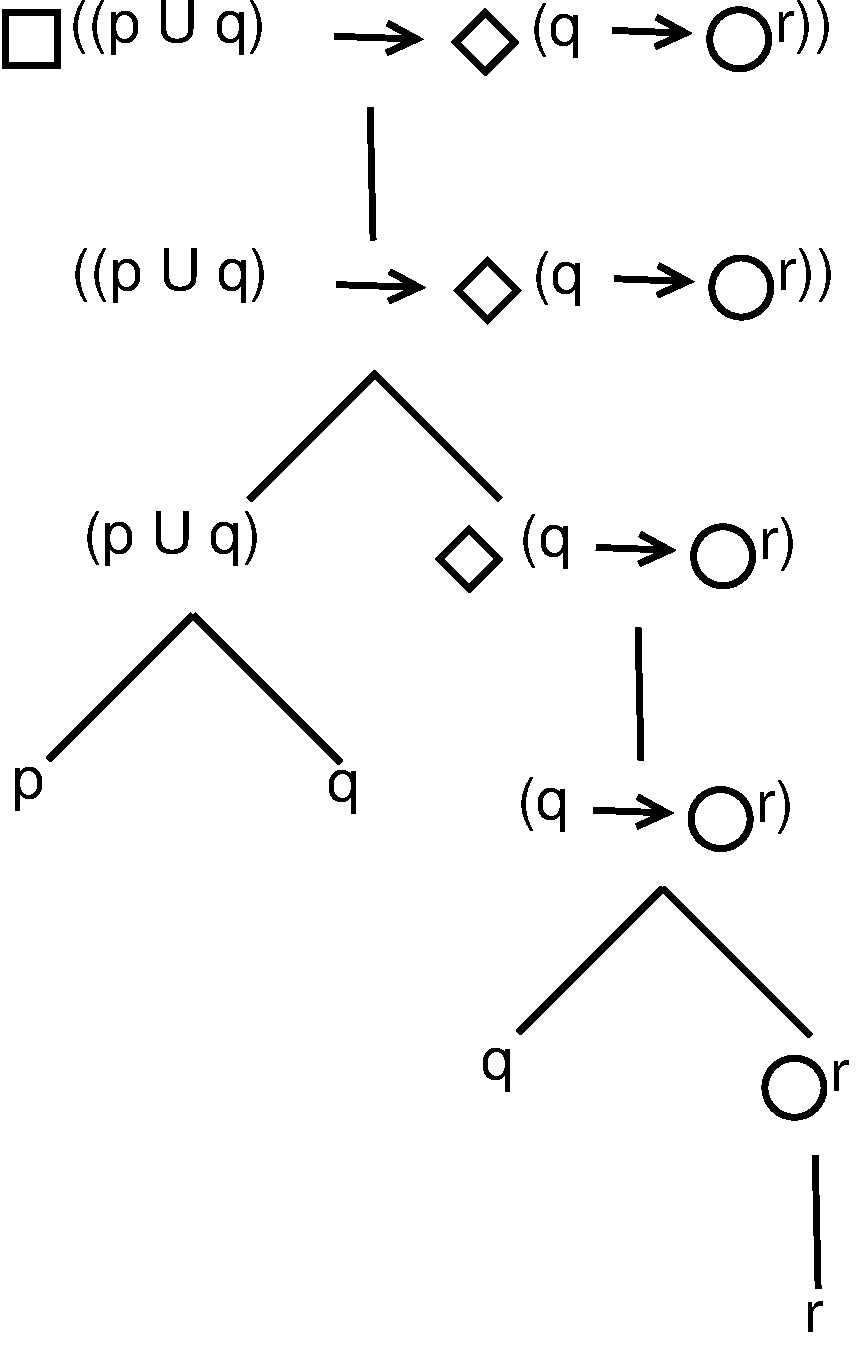
\includegraphics[height=0.3\textheight]{graphics/SubformulaTree}
\label{fig:subformulaTree}
\end{figure}
\\
\qed
\end{myEx}

\begin{description}
\item[Step 2] Walk the tree in breadth-first order to produce a list of subformulae.
\end{description}

\begin{myEx} When we walk the tree in previous example, we get the following subformulae:%The formula $ \varphi = \LTLalways((p \,U q) \rightarrow \LTLeventually(q \rightarrow \LTLnext r)) $ produces subformulae:
\begin{flushleft}
$ \varphi_{1} = \LTLalways((p \,U q) \rightarrow \LTLeventually(q \rightarrow \LTLnext r)) $ \\
$ \varphi_{2} = ((p \,U q) \rightarrow \LTLeventually(q \rightarrow \LTLnext r)) $ \\
$ \varphi_{3} = (p \,U q) $ \\
$ \varphi_{4} = \LTLeventually(q \rightarrow \LTLnext r) $ \\
$ \varphi_{5} = p $ \\
$ \varphi_{6} = q $ \\
$ \varphi_{7} = (q \rightarrow \LTLnext r) $ \\
$ \varphi_{8} = q $ \\
$ \varphi_{9} = \LTLnext r $ \\
$ \varphi_{10} = r $ 
\end{flushleft}
\qed
\end{myEx}

\begin{description}
\item[Step 3] Construct two identical registers called \textit{now} and \textit{next}.  Each register is a one-dimensional array of booleans, where each element corresponds to a formula from the subformulae list, and the length of the array is equal to the length of that list.  Both registers are a permanent breadth-first ordering of the subformula tree.  The first element in the register corresponds to the root of the tree and the last element in the register corresponds to the deepest leaf node of the tree.  The boolean value in each element of the array will hold the truth value that results from evaluating a trace event.\\
\end{description}

\begin{myEx} The now and next registers:\\
\begin{tabular}{cc|c|c|c|c|c|c|c|c|c|c|} &
\multicolumn{1}{c}{} &
\multicolumn{1}{c} {$ \varphi_{1}$} &
\multicolumn{1}{c} {$ \varphi_{2}$} &
\multicolumn{1}{c} {$ \varphi_{3}$} &
\multicolumn{1}{c} {$ \varphi_{4}$} &
\multicolumn{1}{c} {$ \varphi_{5}$} &
\multicolumn{1}{c} {$ \varphi_{6}$} &
\multicolumn{1}{c} {$ \varphi_{7}$} &
\multicolumn{1}{c} {$ \varphi_{8}$} & 
\multicolumn{1}{c} {$ \varphi_{9}$} & 
\multicolumn{1}{c} {$ \varphi_{10}$} \\
\cline{3-12}
& now & $\LTLalways$ & $\rightarrow$ & $U$ & $\LTLeventually$ & $p$ & $q$ & $\rightarrow$ & $q$ & $\LTLnext$ & $r$ \\
\cline{3-12}
\end{tabular}\\
\begin{tabular}{cc|c|c|c|c|c|c|c|c|c|c|} &
\multicolumn{1}{c}{} &
\multicolumn{1}{c} {$ \varphi_{1}$} &
\multicolumn{1}{c} {$ \varphi_{2}$} &
\multicolumn{1}{c} {$ \varphi_{3}$} &
\multicolumn{1}{c} {$ \varphi_{4}$} &
\multicolumn{1}{c} {$ \varphi_{5}$} &
\multicolumn{1}{c} {$ \varphi_{6}$} &
\multicolumn{1}{c} {$ \varphi_{7}$} &
\multicolumn{1}{c} {$ \varphi_{8}$} & 
\multicolumn{1}{c} {$ \varphi_{9}$} & 
\multicolumn{1}{c} {$ \varphi_{10}$} \\
\cline{3-12}
& next & $\LTLalways$ & $\rightarrow$ & $U$ & $\LTLeventually$ & $p$ & $q$ & $\rightarrow$ & $q$ & $\LTLnext$ & $r$ \\
\cline{3-12}
\end{tabular}\\
\qed
\end{myEx}

\begin{description}
\item[Step 4] Before the evaluation phase is performed, the truth values of the \textit{next} register must be initialised.  Traverse the register from the last cell to the first, the initial truth value of the element is the value arrived at when evaluating the subformula over an empty trace ($ \epsilon $).  The semantics are those of the future LTL operators and are given in definition \ref{def:FutureEmptyTraceSemantics}.\\
\end{description}

\begin{myEx} Given the example formula $ \varphi = \LTLalways((p \,U q) \rightarrow \LTLeventually(q \rightarrow \LTLnext r))$ the first cell to be initialised is the cell corresponding to $ \varphi_{10}$, which is the literal r in the subformula tree.  According to semantic rule 1 defined in \ref{def:FutureEmptyTraceSemantics}, a literal over the empty trace evaluates to $ \bot $.  Therefore, after the first cell is evaluated the \textit{next} register looks as follows:

\begin{tabular}{cc|c|c|c|c|c|c|c|c|c|c|} &
\multicolumn{1}{c}{} &
\multicolumn{1}{c} {$ \varphi_{1}$} &
\multicolumn{1}{c} {$ \varphi_{2}$} &
\multicolumn{1}{c} {$ \varphi_{3}$} &
\multicolumn{1}{c} {$ \varphi_{4}$} &
\multicolumn{1}{c} {$ \varphi_{5}$} &
\multicolumn{1}{c} {$ \varphi_{6}$} &
\multicolumn{1}{c} {$ \varphi_{7}$} &
\multicolumn{1}{c} {$ \varphi_{8}$} & 
\multicolumn{1}{c} {$ \varphi_{9}$} & 
\multicolumn{1}{c} {$ \varphi_{10}$} \\
\cline{3-12}
& next & $\LTLalways$ & $\rightarrow$ & $U$ & $\LTLeventually$ & $p$ & $q$ & $\rightarrow$ & $q$ & $\LTLnext$ & $\bot$ \\
\cline{3-12}
\end{tabular}\\
\\
\\
The second cell to be initialised is $\varphi_{9}$, the formula $\LTLnext r$.  Rule 6 says the next operator evaluates to $ \bot $ over the empty trace:

\begin{tabular}{cc|c|c|c|c|c|c|c|c|c|c|} &
\multicolumn{1}{c}{} &
\multicolumn{1}{c} {$ \varphi_{1}$} &
\multicolumn{1}{c} {$ \varphi_{2}$} &
\multicolumn{1}{c} {$ \varphi_{3}$} &
\multicolumn{1}{c} {$ \varphi_{4}$} &
\multicolumn{1}{c} {$ \varphi_{5}$} &
\multicolumn{1}{c} {$ \varphi_{6}$} &
\multicolumn{1}{c} {$ \varphi_{7}$} &
\multicolumn{1}{c} {$ \varphi_{8}$} & 
\multicolumn{1}{c} {$ \varphi_{9}$} & 
\multicolumn{1}{c} {$ \varphi_{10}$} \\
\cline{3-12}
& next & $\LTLalways$ & $\rightarrow$ & $U$ & $\LTLeventually$ & $p$ & $q$ & $\rightarrow$ & $q$ & $\bot$ & $\bot$ \\
\cline{3-12}
\end{tabular}\\
\\
\\
The next cell to be initialised is $\varphi_8$, another literal, therefore it takes the value $\bot$:

\begin{tabular}{cc|c|c|c|c|c|c|c|c|c|c|} &
\multicolumn{1}{c}{} &
\multicolumn{1}{c} {$ \varphi_{1}$} &
\multicolumn{1}{c} {$ \varphi_{2}$} &
\multicolumn{1}{c} {$ \varphi_{3}$} &
\multicolumn{1}{c} {$ \varphi_{4}$} &
\multicolumn{1}{c} {$ \varphi_{5}$} &
\multicolumn{1}{c} {$ \varphi_{6}$} &
\multicolumn{1}{c} {$ \varphi_{7}$} &
\multicolumn{1}{c} {$ \varphi_{8}$} & 
\multicolumn{1}{c} {$ \varphi_{9}$} & 
\multicolumn{1}{c} {$ \varphi_{10}$} \\
\cline{3-12}
& next & $\LTLalways$ & $\rightarrow$ & $U$ & $\LTLeventually$ & $p$ & $q$ & $\rightarrow$ & $\bot$ & $\bot$ & $\bot$ \\
\cline{3-12}
\end{tabular}\\
\\
\\
The formula corresponding to cell $\varphi_7$ is $(q \rightarrow \LTLnext r)$.  The semantics of the implies operator are defined by rule 5: The cell takes the value of $\top$ when the antecedent is $\bot$.  In this case the antecedent is the literal q and the corresponding cell, $\varphi_8$, evaluated to $\bot$ in the previous step.  Therefore $\varphi_7$ takes the value $\top$ because the antecedent evaluates to $ \bot $.  The \textit{next} register is updated to look like:

\begin{tabular}{cc|c|c|c|c|c|c|c|c|c|c|} &
\multicolumn{1}{c}{} &
\multicolumn{1}{c} {$ \varphi_{1}$} &
\multicolumn{1}{c} {$ \varphi_{2}$} &
\multicolumn{1}{c} {$ \varphi_{3}$} &
\multicolumn{1}{c} {$ \varphi_{4}$} &
\multicolumn{1}{c} {$ \varphi_{5}$} &
\multicolumn{1}{c} {$ \varphi_{6}$} &
\multicolumn{1}{c} {$ \varphi_{7}$} &
\multicolumn{1}{c} {$ \varphi_{8}$} & 
\multicolumn{1}{c} {$ \varphi_{9}$} & 
\multicolumn{1}{c} {$ \varphi_{10}$} \\
\cline{3-12}
& next & $\LTLalways$ & $\rightarrow$ & $U$ & $\LTLeventually$ & $p$ & $q$ & $\top$ & $\bot$ & $\bot$ & $\bot$ \\
\cline{3-12}
\end{tabular}\\
\\
\\
This process continues until all the cells of the \textit{next} register have been initialised by evaluation over the empty trace.  The cells in the \textit{now} register are written to by the second phase of the algorithm before they are read, therefore they do not require any initialisation.\\
\\
When the process is complete the two registers appear as follows:\\
\noindent
\begin{tabular}{cc|c|c|c|c|c|c|c|c|c|c|} &
\multicolumn{1}{c}{} &
\multicolumn{1}{c} {$ \varphi_{1}$} &
\multicolumn{1}{c} {$ \varphi_{2}$} &
\multicolumn{1}{c} {$ \varphi_{3}$} &
\multicolumn{1}{c} {$ \varphi_{4}$} &
\multicolumn{1}{c} {$ \varphi_{5}$} &
\multicolumn{1}{c} {$ \varphi_{6}$} &
\multicolumn{1}{c} {$ \varphi_{7}$} &
\multicolumn{1}{c} {$ \varphi_{8}$} & 
\multicolumn{1}{c} {$ \varphi_{9}$} & 
\multicolumn{1}{c} {$ \varphi_{10}$} \\
\cline{3-12}
& next & $\top$ & $\top$ & $\bot$ & $\top$ & $\bot$ & $\bot$ & $\top$ & $\bot$ & $\bot$ & $\bot$\\
\cline{3-12}
\end{tabular}\\
\\
\begin{tabular}{cc|c|c|c|c|c|c|c|c|c|c|} &
\multicolumn{1}{c}{} &
\multicolumn{1}{c} {$ \varphi_{1}$} &
\multicolumn{1}{c} {$ \varphi_{2}$} &
\multicolumn{1}{c} {$ \varphi_{3}$} &
\multicolumn{1}{c} {$ \varphi_{4}$} &
\multicolumn{1}{c} {$ \varphi_{5}$} &
\multicolumn{1}{c} {$ \varphi_{6}$} &
\multicolumn{1}{c} {$ \varphi_{7}$} &
\multicolumn{1}{c} {$ \varphi_{8}$} & 
\multicolumn{1}{c} {$ \varphi_{9}$} & 
\multicolumn{1}{c} {$ \varphi_{10}$} \\
\cline{3-12}
& now & $\LTLalways$ & $\rightarrow$ & $U$ & $\LTLeventually$ & $p$ & $q$ & $\rightarrow$ & $q$ & $\LTLnext$ & $r$ \\
\cline{3-12}
\end{tabular}\\
\\
\qed
\end{myEx}
\noindent That concludes the first phase of the algorithm that produces two registers from an LTL formula.\\  

\section{Evaluation Phase}
\label{sec:EvaluationPhase}
The second phase of the algorithm evaluates the formula over a non-empty trace and is performed for every event in the trace.\\
\begin{description}
%\item[Step 1] When a new event occurs add that event to the end of the trace.

\item[Step 1] Traverse the trace from the last entry to the first, taking each entry from the trace.  With that entry traverse the \textit{now} register from last cell to the first, evaluating the corresponding subformula over the trace entry, according to the operator's semantics from definition \ref{def:FutureNon-emptyTraceSemantics}.  Set the boolean value of the cell to the resulting truth value.

\item[Step 2] next[i] = now[i] for all i ranging from 1..length(now).

\item[Step 3] Repeat steps 2 and 3 with the preceding (earlier) trace entry until arriving at the head of the trace where there is no preceding entry.

\item[Step 4] The final result of evaluating the formula over the trace is found as the truth value of the first cell in the \textit{next} register because this cell corresponds to the root of the subformula tree.\\
\end{description}

Understanding steps 1 and 2 is key to understanding the \RH\ algorithm and how it evaluates the temporal operators of LTL.  There are three elements to understanding these steps, the \textit{next} register, the relation between the \textit{now} register and the \textit{next} register and the order that the trace is evaluated.

To explain how to evaluate a trace event in relation to the registers, we have to adapt the semantics from definition \ref{def:FutureNon-emptyTraceSemantics} to refer to the registers.  We replace $e$ with a reference to the \textit{now} register and $t$ becomes the \textit{next} register.  The subformulae of $ \varphi $ are replaced with references to the corresponding cells within the \textit{now} and \textit{next} registers by the use of indices $i$, $j$, and $k$.  The index $i$ maps to the cell corresponding to the subformula's operator.  Indices $j$ and $k$ map to the cells corresponding to the left and right operands respectively.  The registers are ordered breadth-first, so an operator comes before it's operands in a register, thus $i < j < k$.\\
%The semantics described below are used in step 1 when evaluating a subformula.  They are an adaptation of the semantics found in definition \ref{def:FutureNon-emptyTraceSemantics} but e t is replaced with a reference to the \textit{now} register and t becomes the \textit{next} register.  The subformulae of $ \varphi $ are replaced with references to the corresponding cells within the \textit{now} and \textit{next} registers by the use of indices i, j, and k.  The index i maps to the cell corresponding to the subformulas operator, while indexes j and k map to the cells corresponding to the left and right operands of the subformula respectively.  The registers are a breadth-first ordering of the subformula tree, therefore an operator comes before its operands in a register, thus i $ < $ j and i $ < $ k.\\
\\
For a given trace event $e$, for all $i$ ranging from length(\textit{now})..1, if the $i^{th}$ outermost operator is:
\begin{enumerate}
\item literal l, then \textit{now}[$i$] $ \leftarrow $ (l == $e$)
\item $ \neg $ then \textit{now}[$i$] $ \leftarrow $ NOT(\textit{now}[$j$]).
\item $ \lor $ then \textit{now}[$i$] $ \leftarrow $ \textit{now}[$j$] OR \textit{now}[$k$]. 
\item $ \land $ then \textit{now}[$i$] $ \leftarrow $ \textit{now}[$j$] AND \textit{now}[$k$]. 
\item $ \rightarrow $ then now[$i$] $ \leftarrow $ NOT(\textit{now}[$j$]) OR \textit{now}[$k$]. 
\item $ \LTLnext $ then \textit{now}[$i$] $ \leftarrow $ \textit{next}[$j$].
\item $ \LTLalways $ then \textit{now}[$i$] $ \leftarrow $ \textit{now}[$j$] AND \textit{next}[$i$].
\item $ \LTLeventually $ then \textit{now}[$i$] $ \leftarrow $ \textit{now}[$j$] OR \textit{next}[$i$].
\item U then \textit{now}[$i$] $ \leftarrow $ \textit{now}[$k$] OR (\textit{now}[$j$] AND \textit{next}[$i$]).
\end{enumerate}

The reader may notice that the boolean operators $ \neg, \lor, \land, \rightarrow $ only reference other cells in the \textit{now} register.  This is because the semantics of these operators do not depend on any other events within the trace.  Whereas the semantics of the temporal operators $ \LTLnext, \ \LTLalways,  \ \LTLeventually, \ U $ depend on events that may have occurred elsewhere in the trace so they also reference the \textit{next} register.

The \textit{next} register represents the cumulative evaluations of all trace events after the event currently being evaluated.  Following each evaluation of an event, the cells of the \textit{next} register get set to the corresponding values from the \textit{now} register.  But we can see that evaluation of the \textit{now} register is itself based upon the earlier state of the \textit{next} register.  This circular-referencing process accumulates all prior evaluations into the \textit{next} register.  Because the trace gets evaluated from the latest entry to the earliest, those prior evaluations are all the events that occurred after the current event.  Therefore the evaluation of each event in the trace is based upon the prior evaluation of events that come after.

Evaluating events from latest to earliest explains why the algorithm is limited to implementing only the future LTL operators; when evaluating an event only the evaluations of `future' events are known.

\begin{myEx}
Example evaluation of a trace $t$ that satisfies $ \varphi $
\\*
$ t = \langle p, q, r \rangle $\\
$ \varphi = \LTLeventually((p \,U q) \rightarrow \LTLeventually(q \rightarrow \LTLnext r)) $\\

\textbf{\item[Phase 1] Initialisation}\\
\\
\begin{tabular}{cc|c|c|c|c|c|c|c|c|c|c|} &
\multicolumn{1}{c}{} &
\multicolumn{1}{c} {$ \varphi_{1}$} &
\multicolumn{1}{c} {$ \varphi_{2}$} &
\multicolumn{1}{c} {$ \varphi_{3}$} &
\multicolumn{1}{c} {$ \varphi_{4}$} &
\multicolumn{1}{c} {$ \varphi_{5}$} &
\multicolumn{1}{c} {$ \varphi_{6}$} &
\multicolumn{1}{c} {$ \varphi_{7}$} &
\multicolumn{1}{c} {$ \varphi_{8}$} & 
\multicolumn{1}{c} {$ \varphi_{9}$} & 
\multicolumn{1}{c} {$ \varphi_{10}$} \\
\cline{3-12}
& next & $ \top $ & $ \top $ & $ \bot $ & $ \top $ & $ \bot $ & $ \bot $ & $ \top $ & $ \bot $ & $ \bot $ & $ \bot $ \\
\cline{3-12}
\end{tabular}\\
\\
\begin{tabular}{cc|c|c|c|c|c|c|c|c|c|c|} &
\multicolumn{1}{c}{} &
\multicolumn{1}{c} {$ \varphi_{1}$} &
\multicolumn{1}{c} {$ \varphi_{2}$} &
\multicolumn{1}{c} {$ \varphi_{3}$} &
\multicolumn{1}{c} {$ \varphi_{4}$} &
\multicolumn{1}{c} {$ \varphi_{5}$} &
\multicolumn{1}{c} {$ \varphi_{6}$} &
\multicolumn{1}{c} {$ \varphi_{7}$} &
\multicolumn{1}{c} {$ \varphi_{8}$} & 
\multicolumn{1}{c} {$ \varphi_{9}$} & 
\multicolumn{1}{c} {$ \varphi_{10}$} \\
\cline{3-12}
& now & $\LTLalways$ & $\rightarrow$ & $U$ & $\LTLeventually$ & $p$ & $q$ & $\rightarrow$ & $q$ & $\LTLnext$ & $r$ \\
\cline{3-12}
\end{tabular}\\
\\
\textbf{\item[Phase 2] Evaluation}\\
\subitem \underline{Iteration 1, e = r}
\\
\\
\noindent The evaluation phase begins with the \textit{next} register as below:

\begin{tabular}{cc|c|c|c|c|c|c|c|c|c|c|} &
\multicolumn{1}{c}{} &
\multicolumn{1}{c} {$ \varphi_{1}$} &
\multicolumn{1}{c} {$ \varphi_{2}$} &
\multicolumn{1}{c} {$ \varphi_{3}$} &
\multicolumn{1}{c} {$ \varphi_{4}$} &
\multicolumn{1}{c} {$ \varphi_{5}$} &
\multicolumn{1}{c} {$ \varphi_{6}$} &
\multicolumn{1}{c} {$ \varphi_{7}$} &
\multicolumn{1}{c} {$ \varphi_{8}$} & 
\multicolumn{1}{c} {$ \varphi_{9}$} & 
\multicolumn{1}{c} {$ \varphi_{10}$} \\
\cline{3-12}
& next & $ \top $ & $ \top $ & $ \bot $ & $ \top $ & $ \bot $ & $ \bot $ & $ \top $ & $ \bot $ & $ \bot $ & $ \bot $ \\
\cline{3-12}
\end{tabular}\\
\\
\\
The first cells to be evaluated correspond to subformulae $\varphi_{10}$ down to $\varphi_{5}$, according to rules 1, 5 and 6 from section \ref{sec:EvaluationPhase} these only reference other cells in the \textit{now} register and evaluate as follows:

\begin{tabular}{cc|c|c|c|c|c|c|c|c|c|c|} &
\multicolumn{1}{c}{} &
\multicolumn{1}{c} {$ \varphi_{1}$} &
\multicolumn{1}{c} {$ \varphi_{2}$} &
\multicolumn{1}{c} {$ \varphi_{3}$} &
\multicolumn{1}{c} {$ \varphi_{4}$} &
\multicolumn{1}{c} {$ \varphi_{5}$} &
\multicolumn{1}{c} {$ \varphi_{6}$} &
\multicolumn{1}{c} {$ \varphi_{7}$} &
\multicolumn{1}{c} {$ \varphi_{8}$} & 
\multicolumn{1}{c} {$ \varphi_{9}$} & 
\multicolumn{1}{c} {$ \varphi_{10}$} \\
\cline{3-12}
& now & $\LTLalways$ & $\rightarrow$ & $U$ & $\LTLeventually$ & $ \bot $ & $ \bot $ & $ \top $ & $ \bot $ & $ \top $ & $ \top $ \\
\cline{3-12}
\end{tabular}\\
\\
\\
The $now[4]$ cell corresponds to the subformula $\LTLeventually(q \rightarrow \LTLnext r)$.  Rule 8 defines the semantics of the eventually operator $\LTLeventually$.  The \textit{next} register is required because eventually formulae take the value $ \top $ when the subformula is either true now, or some time in the future.  Therefore $now[4]$ is $ \top $ if $now[7]$ or $next[4]$ is $\top$.  In this case the cell evaluates to $\top$ and the \textit{now} register is updated to appear:

\begin{tabular}{cc|c|c|c|c|c|c|c|c|c|c|} &
\multicolumn{1}{c}{} &
\multicolumn{1}{c} {$ \varphi_{1}$} &
\multicolumn{1}{c} {$ \varphi_{2}$} &
\multicolumn{1}{c} {$ \varphi_{3}$} &
\multicolumn{1}{c} {$ \varphi_{4}$} &
\multicolumn{1}{c} {$ \varphi_{5}$} &
\multicolumn{1}{c} {$ \varphi_{6}$} &
\multicolumn{1}{c} {$ \varphi_{7}$} &
\multicolumn{1}{c} {$ \varphi_{8}$} & 
\multicolumn{1}{c} {$ \varphi_{9}$} & 
\multicolumn{1}{c} {$ \varphi_{10}$} \\
\cline{3-12}
& now & $\LTLalways$ & $\rightarrow$ & $U$ & $\top$ & $ \bot $ & $ \bot $ & $ \top $ & $ \bot $ & $ \top $ & $ \top $ \\
\cline{3-12}
\end{tabular}\\
\\
\\
The $\varphi_{3}$ cell corresponds to the formula $p \,U q$ which is the until temporal operator.  Rule 9 applies to the until operator.  It evaluates $\top$ when the left operand, p, is true now or the right operand, q, is true now and the whole subformula is true in the future.  The cell evaluates $\bot$.

\begin{tabular}{cc|c|c|c|c|c|c|c|c|c|c|} &
\multicolumn{1}{c}{} &
\multicolumn{1}{c} {$ \varphi_{1}$} &
\multicolumn{1}{c} {$ \varphi_{2}$} &
\multicolumn{1}{c} {$ \varphi_{3}$} &
\multicolumn{1}{c} {$ \varphi_{4}$} &
\multicolumn{1}{c} {$ \varphi_{5}$} &
\multicolumn{1}{c} {$ \varphi_{6}$} &
\multicolumn{1}{c} {$ \varphi_{7}$} &
\multicolumn{1}{c} {$ \varphi_{8}$} & 
\multicolumn{1}{c} {$ \varphi_{9}$} & 
\multicolumn{1}{c} {$ \varphi_{10}$} \\
\cline{3-12}
& now & $\LTLalways$ & $\rightarrow$ & $ \bot $ & $ \top $ & $ \bot $ & $ \bot $ & $ \top $ & $ \bot $ & $ \bot $ & $ \top $ \\
\cline{3-12}
\end{tabular}\\
\\
\\
The $\varphi_{2}$ cell is the implies formula $(p \,U q) \rightarrow \LTLeventually(q \rightarrow \LTLnext r)$.  By Rule 5 the cell evaluates to $\top$.

\begin{tabular}{cc|c|c|c|c|c|c|c|c|c|c|} &
\multicolumn{1}{c}{} &
\multicolumn{1}{c} {$ \varphi_{1}$} &
\multicolumn{1}{c} {$ \varphi_{2}$} &
\multicolumn{1}{c} {$ \varphi_{3}$} &
\multicolumn{1}{c} {$ \varphi_{4}$} &
\multicolumn{1}{c} {$ \varphi_{5}$} &
\multicolumn{1}{c} {$ \varphi_{6}$} &
\multicolumn{1}{c} {$ \varphi_{7}$} &
\multicolumn{1}{c} {$ \varphi_{8}$} & 
\multicolumn{1}{c} {$ \varphi_{9}$} & 
\multicolumn{1}{c} {$ \varphi_{10}$} \\
\cline{3-12}
& now & $\LTLalways$ & $ \top $ & $ \bot $ & $ \top $ & $ \bot $ & $ \bot $ & $ \top $ & $ \bot $ & $ \bot $ & $ \top $ \\
\cline{3-12}
\end{tabular}\\
\\
\\
The final cell $ \varphi_{1}$ is the third temporal operator of the formula, the always operator.  By Rule 7 the cell evaluates to $\top $ when the subformula is $\top$ now and $\top$ for all following trace entries.  Therefore evaluation of this formula is the conjunction of $now[2]$ with $next[1]$.  It takes the value $\top$.

\begin{tabular}{cc|c|c|c|c|c|c|c|c|c|c|} &
\multicolumn{1}{c}{} &
\multicolumn{1}{c} {$ \varphi_{1}$} &
\multicolumn{1}{c} {$ \varphi_{2}$} &
\multicolumn{1}{c} {$ \varphi_{3}$} &
\multicolumn{1}{c} {$ \varphi_{4}$} &
\multicolumn{1}{c} {$ \varphi_{5}$} &
\multicolumn{1}{c} {$ \varphi_{6}$} &
\multicolumn{1}{c} {$ \varphi_{7}$} &
\multicolumn{1}{c} {$ \varphi_{8}$} & 
\multicolumn{1}{c} {$ \varphi_{9}$} & 
\multicolumn{1}{c} {$ \varphi_{10}$} \\
\cline{3-12}
& now & $ \top $  & $ \top $ & $ \bot $ & $ \top $ & $ \bot $ & $ \bot $ & $ \top $ & $ \bot $ & $ \bot $ & $ \top $ \\
\cline{3-12}
\end{tabular}\\
\\
\\
\noindent Once the \textit{now} register has been evaluated the values in the \textit{next} register are overwritten with those from the \textit{now} register and it appears as:

\begin{tabular}{cc|c|c|c|c|c|c|c|c|c|c|} &
\multicolumn{1}{c}{} &
\multicolumn{1}{c} {$ \varphi_{1}$} &
\multicolumn{1}{c} {$ \varphi_{2}$} &
\multicolumn{1}{c} {$ \varphi_{3}$} &
\multicolumn{1}{c} {$ \varphi_{4}$} &
\multicolumn{1}{c} {$ \varphi_{5}$} &
\multicolumn{1}{c} {$ \varphi_{6}$} &
\multicolumn{1}{c} {$ \varphi_{7}$} &
\multicolumn{1}{c} {$ \varphi_{8}$} & 
\multicolumn{1}{c} {$ \varphi_{9}$} & 
\multicolumn{1}{c} {$ \varphi_{10}$} \\
\cline{3-12}
& next & $ \top $  & $ \top $ & $ \bot $ & $ \top $ & $ \bot $ & $ \bot $ & $ \top $ & $ \bot $ & $ \bot $ & $ \top $ \\
\cline{3-12}
\end{tabular}\\
\\
\\
\subitem \underline{Iteration 2, e = q}

\begin{tabular}{cc|c|c|c|c|c|c|c|c|c|c|} &
\multicolumn{1}{c}{} &
\multicolumn{1}{c} {$ \varphi_{1}$} &
\multicolumn{1}{c} {$ \varphi_{2}$} &
\multicolumn{1}{c} {$ \varphi_{3}$} &
\multicolumn{1}{c} {$ \varphi_{4}$} &
\multicolumn{1}{c} {$ \varphi_{5}$} &
\multicolumn{1}{c} {$ \varphi_{6}$} &
\multicolumn{1}{c} {$ \varphi_{7}$} &
\multicolumn{1}{c} {$ \varphi_{8}$} & 
\multicolumn{1}{c} {$ \varphi_{9}$} & 
\multicolumn{1}{c} {$ \varphi_{10}$} \\
\cline{3-12}
& next & $ \top $ & $ \top $ & $ \bot $ & $ \top $ & $ \bot $ & $ \bot $ & $ \top $ & $ \bot $ & $ \bot $ & $ \top $ \\
\cline{3-12}
\end{tabular}\\

\begin{tabular}{cc|c|c|c|c|c|c|c|c|c|c|} &
\multicolumn{1}{c}{} &
\multicolumn{1}{c} {$ \varphi_{1}$} &
\multicolumn{1}{c} {$ \varphi_{2}$} &
\multicolumn{1}{c} {$ \varphi_{3}$} &
\multicolumn{1}{c} {$ \varphi_{4}$} &
\multicolumn{1}{c} {$ \varphi_{5}$} &
\multicolumn{1}{c} {$ \varphi_{6}$} &
\multicolumn{1}{c} {$ \varphi_{7}$} &
\multicolumn{1}{c} {$ \varphi_{8}$} & 
\multicolumn{1}{c} {$ \varphi_{9}$} & 
\multicolumn{1}{c} {$ \varphi_{10}$} \\
\cline{3-12}
& now & $ \top $ & $ \top $ & $ \top $ & $ \top $ & $ \bot $ & $ \top $ & $ \top $ & $ \top $ & $ \top $ & $ \bot $ \\
\cline{3-12}
\end{tabular}\\
\\
\\
\subitem \underline{Iteration 3, e = p}

\begin{tabular}{cc|c|c|c|c|c|c|c|c|c|c|} &
\multicolumn{1}{c}{} &
\multicolumn{1}{c} {$ \varphi_{1}$} &
\multicolumn{1}{c} {$ \varphi_{2}$} &
\multicolumn{1}{c} {$ \varphi_{3}$} &
\multicolumn{1}{c} {$ \varphi_{4}$} &
\multicolumn{1}{c} {$ \varphi_{5}$} &
\multicolumn{1}{c} {$ \varphi_{6}$} &
\multicolumn{1}{c} {$ \varphi_{7}$} &
\multicolumn{1}{c} {$ \varphi_{8}$} & 
\multicolumn{1}{c} {$ \varphi_{9}$} & 
\multicolumn{1}{c} {$ \varphi_{10}$} \\
\cline{3-12}
& next & $ \top $ & $ \top $ & $ \top $ & $ \top $ & $ \bot $ & $ \top $ & $ \top $ & $ \top $ & $ \top $ & $ \bot $ \\
\cline{3-12}
\end{tabular}\\

\begin{tabular}{cc|c|c|c|c|c|c|c|c|c|c|} &
\multicolumn{1}{c}{} &
\multicolumn{1}{c} {$ \varphi_{1}$} &
\multicolumn{1}{c} {$ \varphi_{2}$} &
\multicolumn{1}{c} {$ \varphi_{3}$} &
\multicolumn{1}{c} {$ \varphi_{4}$} &
\multicolumn{1}{c} {$ \varphi_{5}$} &
\multicolumn{1}{c} {$ \varphi_{6}$} &
\multicolumn{1}{c} {$ \varphi_{7}$} &
\multicolumn{1}{c} {$ \varphi_{8}$} & 
\multicolumn{1}{c} {$ \varphi_{9}$} & 
\multicolumn{1}{c} {$ \varphi_{10}$} \\
\cline{3-12}
& now & $ \top $ & $ \top $ & $ \top $ & $ \top $ & $ \top $ & $ \bot $ & $ \top $ & $ \bot $ & $ \bot $ & $ \bot $ \\
\cline{3-12}
\end{tabular}\\
\\
\\
\subitem \underline{Final state}

\begin{tabular}{cc|c|c|c|c|c|c|c|c|c|c|} &
\multicolumn{1}{c}{} &
\multicolumn{1}{c} {$ \varphi_{1}$} &
\multicolumn{1}{c} {$ \varphi_{2}$} &
\multicolumn{1}{c} {$ \varphi_{3}$} &
\multicolumn{1}{c} {$ \varphi_{4}$} &
\multicolumn{1}{c} {$ \varphi_{5}$} &
\multicolumn{1}{c} {$ \varphi_{6}$} &
\multicolumn{1}{c} {$ \varphi_{7}$} &
\multicolumn{1}{c} {$ \varphi_{8}$} & 
\multicolumn{1}{c} {$ \varphi_{9}$} & 
\multicolumn{1}{c} {$ \varphi_{10}$} \\
\cline{3-12}
& next & $ \top $ & $ \top $ & $ \top $ & $ \top $ & $ \top $ & $ \bot $ & $ \top $ & $ \bot $ & $ \bot $ & $ \bot $ \\
\cline{3-12}
\end{tabular}\\
\\
\\
$ t \models \varphi = next[1] = \top $
\qed
\end{myEx}

This concludes our description of how the \RH\ algorithm operates.



\chapter{Android Platform}
\label{chap:Android Platform}

In this chapter, we explore the workings of the Android platform, how each layer in the stack contributes to Android security and safe communication between processes.  We use the first chapter from the Nikolay Elenkov book `Android Security Internals' \cite{AndroidSecurityInternals} as our source and guidance.

\begin{figure}[h]
  \centering
  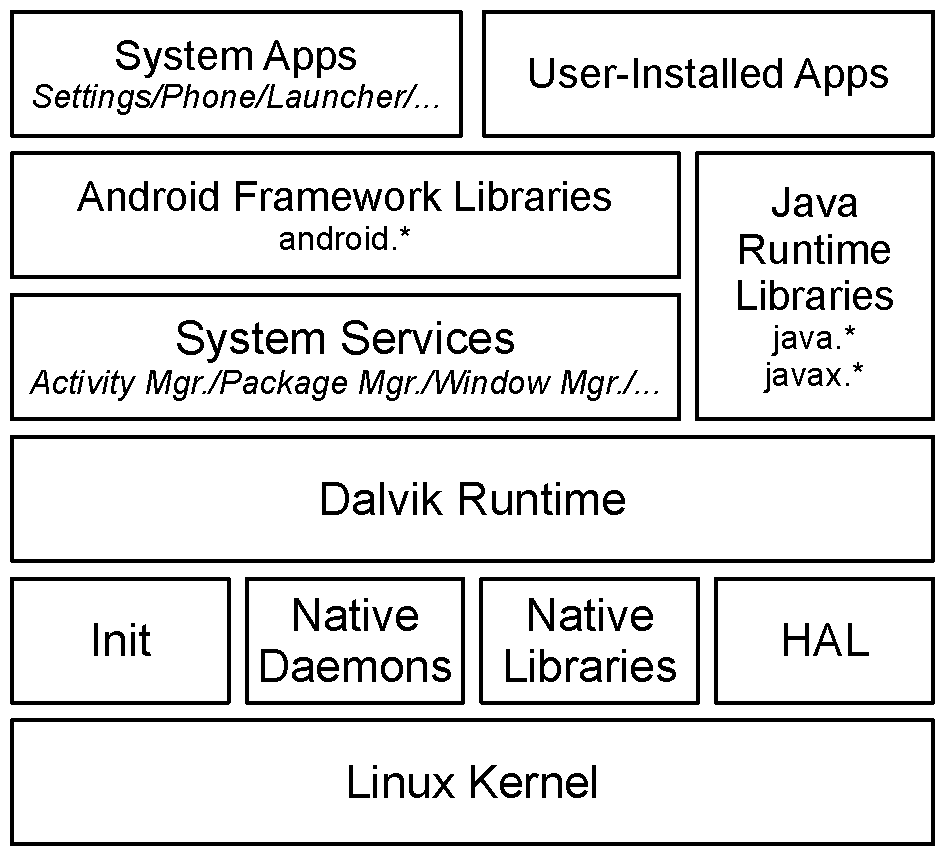
\includegraphics[width=0.5\textwidth]{graphics/AndroidStack.pdf}
  \caption{The Android architecture}
  \label{fig:AndroidStack}
\end{figure}

\section{Linux}
\label{sec:Linux}

At its core, Android is built on the Linux kernel with some modifications specific to Android.  The standard security mechanisms provided by Linux enforce process isolation through sandboxing and user-based file access permissions.  Android adds two more features to the standard Linux kernel.  First, a feature called paranoid networking forces processes to have permission to use sockets. The second is an IPC system called Binder that underpins all IPC methods in Android.  We describe Binder in more detail in section \ref{sec:IPC} and permissions in \ref{sec:Permissions}.

Above the kernel layer is the Init binary, native daemons, native libraries, and a hardware abstraction layer (HAL).  The Init binary contains the first process started by Linux, the zygote process, and native daemons run in the background providing services and functionality.  The HAL is a daemon that maintains a realtime database of devices connected to the system and provides an API that applications can use to discover, monitor and invoke operations on devices. The Linux native libraries are code collections, such as the standard C routines or encryption functions, for application programmers.

\subsection{Sandboxing}
\label{sec:Sandboxing}

The sandboxing feature of Linux gives each installed android package a unique userId.  A Linux process can only execute code with the same userId, so different packages get forced to run in different processes.  Linux uses memory management to separate processes into their own address spaces.  By doing so, a process is unable to reference other processes address space.  They cannot corrupt each other's memory, read, write or in any way communicate with each other directly via memory.  They are also unable to reference memory owned by operating system processes that run in protected mode.  Thus, they cannot insert code into the operating systems memory space to execute it in protected mode. 
  
\subsection{FileAccessPermissions}
\label{sec:FileAccessPermissions}  

The second feature provided by the Linux kernel is that of file access permissions.  Files are associated with an owner's userId (UID) and a groupId (GID) along with three tuples of read, write, execute permissions.  The first tuple is the owner's permission, the second is the permissions granted to the group that the owner is a member of, and the final tuple is the permissions for all other users.  When consideration gets given to setting these tuples, they can control all access to files and prevent unwanted access by unknown users.  In addition, the Linux kernel extends this security mechanism to hardware drivers by exposing them as pseudo-files.  Linux file access rules can be quite effective for restricting access to resources when configured to do so.\\

\noindent
These two features stem from using unique userIds per package and the rule that a process can only execute code owned by a single UID.  But as is often the case with security, there is a built-in way to circumvent this by sharing userIds.  The Linux kernel allows packages to share UIDs with other packages.  But, both packages must specifically request this, and they must both get signed by the same party.  So, for the most part, packages are separated from each other but, the shared UID feature does open the door to malicious activity via inter-process communication within the same sandbox.

\section{Dalvik Virtual Machine}
\label{sec:Dalvik Virtual Machine}

Android is mainly developed in Java but there are a number of diversions from the standard Java stack that improve its use on mobile devices.  Diversions stem from the limited electrical energy available on a mobile device.

\begin{enumerate}
\item Java code is compiled to device-independent Dalvik executable code rather than Java bytecode.
\item Dalvik code is executed by the Dalvik Virtual Machine rather than the standard Oracle JVM.
\item The DVM is a register-based platform while the JVM is stack-based.
\item The instruction sets are different.
\end{enumerate}

This results in code that can be more efficiently executed by the DVM but it also increases the amount of code and that leads to a greater memory requirement.  Despite there being more code to execute, there is still a net gain to processing efficiency because the processor can load code quicker than it can execute so if execution time can be swapped for loading time there is a performance gain.

The trade-off between processor efficiency and memory requirement is beneficial on a mobile device because energy is limited so the device must be designed to reduce battery drain.  Processors that consume less energy tend to have less processing capability but the DVM requires less processing capability to get adequate performance from applications therefore a less powerful processor is still adequate.  Although additional memory is required it is only for code rather than data and code occupies small amount of memory compared to data so the increase in memory usage is small.  Thus overall energy usage can be minimised by using a processor with less processing capability even at the expense of increased memory capacity.

Further optimisations are made to the .dex code when the application is installed on the device.  At this point the processor that the code will execute on is known so the code can be compiled into the native instruction set for that processor.  The native code is known as optimised dex.  Java bytecode on the other hand is famously just-in-time compiled to native code on the first execution and cached for subsequent executions but the native code is lost if it is unloaded from memory.  Just-in-time compilation must be repeated every time code is loaded for execution while compiling at installation-time only occurs once.

\section{Android}
\label{sec:Android}

Sitting upon the DVM come the Java Runtime Libraries (java.* and javax.* packages) and Android system services such as the Activity Manager, Package Manager and Window Manager.  The JRL packages make use of the native libraries of the layer below through the Java Native Interface (JNI).  The system services form the core of Android and implement most of the fundamental features such as display, touch screen support, telephony and network connectivity.  These are mainly implemented in Java with some fundamental parts in native code.  Android takes advantage of standard Linux process-isolation which enforces a separate address space for all processes and prevents them from directly accessing each others memory.

\subsection{Permissions}
\label{sec:Permissions}

Further security is provided by an additional permissions system that is specific to the Android operating system.  Access to protected features of the operating system such as the ability to connect to the internet, make calls, use the GPS or camera are restricted to applications that request permission to use them during the installation of the application.  The developer requests permissions by stating the requirement to use a protected feature in the applications manifest.  The manifest is an xml file that accompanies the application.  It informs the operating system, tools used to built the application and repositories like Google Play of essential information about the app.  Among the information provided in the manifest are the permissions required to access protected parts of the device that the app will run on.  Android reads the manifest on installation of the software and asks the user if they wish to grant the application the permissions it requires.  Once an application has been granted permissions it will be denied further permissions at runtime.  There are four protection levels for each feature.  Normal and dangerous protection level are granted to an application if the user agrees to allow that during installation.  The Signature protection level requires the signature of the package being installed to match the signature of the package that created the permission.  The signature-or-system level is less restrictive in that it will also allow the package to be installed in the system image.

While the permissions scheme does provide some security, it suffers from the typical problem that the application is unlikely to function if it does not get permission to use all the features it requests.  So if the user decides they do not want to allow a certain permission they will have to abandon installation of the app.  When the user is faced with making this decision they often agree to the requests regardless of the dangers simply because they have no alternative but to use the software.  This is akin to agreeing the terms of a license without reading the lengthy document simply because it is inconvenient, unintelligible or it leaves the user with no option if they do not like certain parts of the agreement.  Furthermore once the user has agreed permissions and app has been installed, there is no way to tell what the features are being used for.  For the most part the use will be benign and any malicious use will be infrequent enough to go unnoticed.
 
\subsection{Interprocess Communication}
\label{sec:IPC}

The need to keep applications and their components separate is key to security and robustness, and is therefore a necessary consideration but, at the same time, it is contrary to the need to provide a feature rich experience to the user.  If applications and the components within them have the ability to collaborate with each other then the device becomes a more powerful tool.  Therefore, Android has overt communication channels specifically for communication between applications.

Android includes a controlled communication mechanism called Binder that underpins all inter-process communication in Android.  Binder is an interface exposed by the kernel as the /dev/binder device and implemented by the Binder kernel driver.  It is an implementation of OpenBinder which is similar in concept to COM or CORBA but does not support RPC.  The kernel implementation of Binder allows it to manage some of the address space of each process and write data into that memory area.  When a process sends a message to another via Binder, Binder copies the message to the destination processes managed memory area and notifies the process that is has a message.  The process can then consume the message from that memory area.  IPC via Binder is performed through transactions that include a reference to the object being called, a method id, a buffer containing parameter data, a processId and effective-userId.  The PID and UID are added to the transaction by Binder not the callee and therefore it is impossible for the callee to spoof these ids.  This prevents a process gaining the privileges of another process by using another processes ids.

Android builds a variety of more specific IPC channels upon Binder.  One such channel is the system of intents.  An intent can be thought of as a command that is sent to a particular receiver or as an event that notifies listeners when something they are interested in has happened.  If an SMS message is received then an Android component can publish an intent to inform listeners of the incoming SMS.  Listeners subscribe to intents and can take action when they receive notification of an event.

Higher level IPC channels called Messengers, Content Providers and Services are built on Binder.  Services allow an Android app to provide features to other apps by exposing components for external use.  Components have interfaces defined in the Android Interface Definition Language (AIDL).  Proxies and stubs are generated as java objects that implement the interfaces and delegate parameter marshaling/unmarshaling to Binder.  Components have an 'exported' property that can be set to false to prevent apps with different UIDs from using that component.  This system has a weaknesses due to there being a default encapsulation policy that dictates whether a component is exported if the developer has not given any specific instruction.  If the developer has not purposefully set the exported property then the component is exported by default.  Messengers are objects that enable message-based communication and Content Providers are components that expose data management interfaces.  


%There are a number of different security mechanisms provided by the Android operating system.  Firstly, at its core, is a Linux kernel that enforces the POSIX security features of process isolation sandboxing and user-based permissions.

%The sandboxing feature of Linux gives each installed android package a unique userId and a Linux process can only execute code with a single userId.  This means different packages must run in different processes.  Linux uses a memory management unit to separate processes into their own address spaces.  By doing this a process is unable to reference another processes address space so they cannot corrupt each others memory, read, write or in any way communicate with each other directly via memory.  They are also unable to reference memory owned by operating system processes that run in protected mode, thus they are unable to insert they own code into an operating systems memory space in order to have it executed in protected mode.  
%  
%The second feature provided by the Linux kernel is that of file access permissions.  Files are associated with an owners userId (UID) and a groupId (GID) along with three tuples of read, write, execute permissions.  The first tuple is the owners permission, the second is the permissions granted to the group the owner is a member of and the final tuple is the permissions for all other users.  Considered settings for these tuples controls all access to files and can be used to prevent unwanted access by unknown users.  The Linux kernel extends this security mechanism to hardware drivers by exposing them as pseudo-files.  This means the Linux files access rules can be used to quite effectively restrict access to resources when configured to do so. 
%
%These two features stem from the use of userIds that are unique per package and the rule that a process can only execute code owned by a single UID.  But as is often the case with security there is a built-in way to circumvent this by sharing userIds.  The Linux kernel allows a package to share a UID with another package but it must be specifically requested by both packages and they must be signed by the same party.  So for the most part packages are separated from each other in sandboxes but the shared UID feature does open the door to malicious activity via inter-application communication within the same sandbox. 

%Further security is provided by a permissions system that is specific to the Android operating system.  Access to protected features of the operating system such as the ability to connect to the internet, make calls, use the GPS or camera are restricted to applications that requested permission to use them during the installation of the application.
%
%There are four protection levels for each feature.  Normal and dangerous protection level are granted to an application if the user agrees to allow that during installation.  The Signature protection level requires the signature of the package being installed to match the signature of the package that created the permission.  The signature-or-system level is less restrictive in that it will also allow the package to be installed in the system image.  Once an application has been granted permissions they will be denied further permissions at runtime.  While this system does attempt to provide some security it suffers from the typical problem that the application is unlikely to function if it does not get permission to use all the features it requests.  So if the user decides they do not want to allow a certain permission they will have to abandon installation of the app.  When the user is faced with making this decision they often agree to the requests regardless of the dangers simply because they have no alternative but to use the software.  This is akin to agreeing the terms of a license without reading the lengthy document simply because it is inconvenient, unintelligible or it leaves the user with no option if they do not like certain parts of the agreement.  Furthermore once the user has agreed permissions and app has been installed, there is no way to tell what the features are being used for.  For the most part the use will be benign and any malicious use will be infrequent enough to go unnoticed.
% 
%An Android app can provide services to other apps by exposing components for external use.  Components have an 'exported' property that can be set to false to prevent apps with different UIDs from using that component.  This system has a weaknesses due to there being a default encapsulation policy that dictates whether a property is exported if the developer has not given any  specific instruction.  Components may be exported by default if the developer has not purposefully set the exported property.  

%Notes

%Android built on Linux kernel with some additions - Binder IPC and paranoid networking which requires permissions for socket usage.
%
%Onto that is a native userspace, including native daemons and libraries and the init binary which is the first process started.
%
%Next is the Dalvik VM - Androids current Java VM.  Cannot run Java bytecode directly.  The native input format is DEX (Dalvik Executable).  .dex files are packaged inside .jar files or inside Android .apk files.  The Dalvik VM is register-based rather stack-based as in the Oracle JVM and uses a different instruction set.  Register based VMs can be interpreted more efficiently due to generally less instructions.  Most .dex code is converted to device-dependent native code called optimized dex (.odex) upon installation.

%Above that is the Java Runtime Libraries (java.* and javax.* packages).  These packages make use of the native libaries of the lower layer by using the Java Native Interface (JNI).
%
%Sitting upon that layer come system services such as the Activity Manager, Package Manager and Window Manager.  These are the core of Android and implement most of the fundamental features such as display, touch screen support, telephony, network connectivity.  Mainly implemented in Java fundamentals in native code.  System services provide remote interfaces through Binder to be called by other services and applications.
%
%Android Process follow standard Linux process-isolation.  By having separate address spaces and being prevented from directly accessing each others memory.
%
%An IPC mechanism called Binder is provided as a controlled means for processes to communicate and offer services.  It is an implementation of OpenBinder which is similar to COM or CORBA but does not support RPC.  Binder is an interface exposed by the kernal as the /dev/binder device and implemented by the Binder kernel driver.  IPC calls go through the binder driver.  The kernel implementation of Binder allows it to manage some of the address space of each process and write data into that memory area.  When a process sends a message to another via Binder, Binder copies the message to the destination processes managed memory area and notifies the process that is has a message.  The process can consume the message from that memory area.
%
%Intents, Messengers and Content Providers are all higher level IPC abstractions that are built upon the Binder mechanism.
%
%Intents - commands to components with associated data.
%Messengers - objects that enable message-based communication.
%Content Providers - components that expose data management interfaces.
%
%Services written with Android Interface Definition Language (AIDL) interfaces are exposed as java objects by generating stubs and proxies that delegate to Binder and perform parameter marshaling/unmarshaling for what is otherwise typeless.
%
%Calls to objects via Binder a performed through a Binder transaction that includes a reference to the object being called, a method id, buffer containing parameter data and a process id and effective user id that is added by Binder and therefore impossible to spoof by the callee.  It is important to prevent a process gain the privileges of another process by using a fake pid or uid because user permissions are central to the Android security model.

 






  
\chapter{Xposed Framework}
\label{chap:Xposed Framework}

The Xposed framework is a third-party framework we use to record the activities of applications running on Android.  It does so by intercepting methods called by processes.  Here we explain the origin of the Xposed framework, how it works, how to prepare a development environment for writing an Xposed module, then we develop a bare-bones example module.

\section{Origins}
\label{sec:Origins}

The Xposed framework for Android was developed by someone we only known by the pseudonym rovo89 \cite{rovo89}.  The first release was in 2012, and development by rovo89 continued until 2018, after which other authors have taken it forward.  The version of Xposed used in this research is version 89 of the software development kit.  It was the latest stable version when the project was started and is compatible with Android up to version 7.1.1.  The version of Android chosen in the research is version 6, which is purposefully an early version.  We chose an earlier version of Android as the target so that a greater range of devices can run the software.

\section{The Zygote Process}
\label{sec:The Zygote Process}

To understand how the framework intercepts method calls, we must understand that all processes in Android get forked from a single process started when the device boots, the zygote process.

The term zygote got borrowed from biology.  A zygote is the first cell formed after fertilisation of a female gamete by a male gamete.  All cells in a multicellular organism are duplicates that stem from the zygote cell.  The term is used in Android to name the first process launched by Android that all other processes get forked from.

The Xposed framework replaces the standard zygote with a modified zygote.  The modified zygote notifies Xposed modules when methods they specify get called.  Any identified method can get specified, even one identified via disassembly.  The ability gets duplicated to all running processes because they are all forked from the zygote.  Thus any identifiable method, called by any and all processes, can be intercepted.

Our software is interested in intercepting operating system calls to read the contacts list.  When that call gets intercepted, our software will record that the call got made, some necessary details, then allow it to continue.

\section{Requirements}
\label{sec:Requirements}

In order to use the Xposed framework the device does have to be rooted.  Rooting allows user processes to have the administrative permissions of a superuser and thus gain privileged control over the device that would otherwise not be possible.  This is necessary so that the Xposed framework can modify the zygote process.  The Xposed framework does this by replacing the \path{/system.bin/app_process} with it's own extended \path{app_process} and to do that root access is required.

Although rooting the device may present a hurdle to casual users, some of the latest Android phones allow the user to root the phone just by enabling a setting in the UI.  Studies of the number of rooted Android devices vary significantly.  In 2017 Kaspersky quoted a global average of only 7.6\% of Android devices were rooted \cite{KaperskyRootedDevices}.  While a 2014 survey conducted by Chinese company Tencent, claims of 8959 users in China, 80\% rooted their devices \cite{CIWRootedDevices}.  It is often assumed that rooted devices are more open to security attacks because malicious software can exploit superuser rights.  While it is true that a rooted device is easier to exploit, a study by Semantic \cite{InsightsIntoRooted} found that there is no increase in malware on rooted devices.  No evidence is presented to why this is, but it may be because the expertise and motivation required to root a device selects people who are also security conscious.  At the very least, the requirement for the device to be rooted should not stop our proposed system being used by professionals to screen applications.

\section{Development and Test Environments}
\label{sec:Development and Test Environments}

Android Studio version 4.1.3 was used to develop this project, versions for all major operating systems can be found at:\\
\url{https://developer.android.com/studio#downloads}\\
\\
It is strongly recommended that development testing is done on an Android emulator because faults in an Xposed module can result in the operating system of the test environment being damaged to the extent that it requires a factory reset.  We discovered that the Xposed framework does not install correctly on the standard Android Virtual Machine included with Android Studio.  Instead, an alternative AVM called GenyMotion, version 3.2.0, was used.\\
\\
GenyMotion requires virtualisation software to be installed first that can be found at:\\
\url{https://www.virtualbox.org/wiki/Downloads}\\
\\
\\
Once Virtual Box is installed GenyMotion can be installed from this location:\\
\url{https://www.genymotion.com/download/}\\
\\
Finally Android Studio Plugins can be installed from here:\\
\url{https://www.genymotion.com/plugins/}

\section{Preparing the Android Device}
\label{sec:Preparing the Android device}

In order to be able to develop and run an Xposed module on an Android device the device must be rooted.  The following section describes how to use a Windows platform to root an Android device and install the Xposed framework.  The device used in this project was the Motorola G4 Play.  Rooting a different device will require some different steps.  To root the device we will install a tool called SuperSU onto the device, and to do this we require a recovery tool called TWRP to be installed on the device first, and to install TWRP we must unlock fastboot mode on the device.

\subsection{Enabling Developer Options}
\label{sec:Enabling developer options on the device}

On the Android device go to Settings \textgreater\ System \textgreater\ About phone\\
\indent Tap Build Number seven times to enable the developer options menu.  You may also have to tap in your PIN for verification.\\
\\
Go to Settings \textgreater\ Developer Options\\
\indent Toggle the Developer options switch to On if it is not already\\
\indent Enable USB Debugging\\
\indent Enable OEM Unlocking

\subsection{Installing Android Device Drivers on a Windows Platform}
\label{sec:Installing Android device drivers on the Windows platform}

Communication between a Windows PC and the Android device is via USB.  It requires drivers on the PC, and the drivers require the Android SDK.\\  
\\
Download and install the Android SDK onto the PC from here:\\
\url{https://developer.android.com/studio}\\
\\
Once the SDK is installed download and install USB drivers for Motorola onto the Windows platform from here:\\
\url{https://support.motorola.com/us/en/solution/MS88481}

\subsection{Unlocking the Bootloader}
\label{sec:Unlocking the Bootloader}

Rooting the device requires a recovery tool called TWRP to be installed on it.  This is done using the Android bootloader to start the device in fastboot mode and update the firmware.  The bootloader is responsible for loading the Android operating system and is normally invisible to the user.  Unlock the bootloader on Motorola devices by following the instructions below.  If the reader uses a device from another manufacturer, they must investigate how to do so with their specific manufacturer.\\
\\
\\
For a Motorola device, create a developer account with Motorola here:\\
\url{https://accounts.motorola.com/ssoauth/login?TARGET=https://motorola-global-portal.custhelp.com/cc/cas/sso/redirect/standalone\%2Fbootloader\%2Funlock-your-device-b}\\
\\
Then follow the instructions here:\\
\url{https://motorola-global-portal.custhelp.com/app/standalone/bootloader/unlock-your-device-b}\\
\\
An unlock key will be sent to the email account you register with the developer account.  Follow the link in the email to further instructions here:\\
\url{https://motorola-global-portal.custhelp.com/app/standalone/bootloader/unlock-your-device-c}

\subsection{Installing the TWRP Recovery Tool}
\label{sec:Installing the recovery tool}

Now the bootloader is unlocked, you can boot into fastboot mode and alter the device's flash memory.  Fastboot consists of three parts:\\
Pre-installed software on the device that is available when the bootloader is unlocked.\\
A utility on the PC.\\
A protocol that allows the PC and the Android device to communicate via USB.\\
\\
Download and install the mfastboot utility, version 1.4.3, from here:\\
\url{https://forum.xda-developers.com/showthread.php?p=42407269#post42407269}\\

\noindent Now your PC can modify the devices flash memory partitions.  We will use fastboot mode to install the TWRP recovery tool, then use TWRP to install custom firmware onto the device.\\
\\
Download TWRP, version 3.1.1, onto the PC from here:\\
\url{https://forum.xda-developers.com/devdb/project/dl/?id=25597}\\
\\
The file on the PC will be named something like: twrp-harpia-3.1.1-r1.img.  Now we will install TWRP from the PC onto the device.\\

\noindent Restart the device in fastboot mode by first shutting it down, then start the device by holding the power button and the volume control buttons together.  The device will bootup and display the fastboot screen.  Various pieces of information about the device, such as the serial number, will get displayed.  It should also say that the device is unlocked.\\

\noindent Copy the twrp-harpia-3.1.1-r1.img file to the folder on the PC where mfastboot is installed, open a command window from the mfastboot installation folder and execute the command:
\begin{verbatim}mfastboot flash recovery twrp-harpia-3.1.1-r1.img\end{verbatim}

\noindent Mfastboot will display 'waiting for device'.  Attach the device to the PC via a USB cable.  Mfastboot will detect the device and install TWRP.  When installation is complete, use the volume controls to select recovery mode, then press the power button to boot into the TWRP recovery tool.\\
\\
Select reboot from TWRP and the device will reboot into system mode.
	
\subsection{Rooting the Android Device}
\label{sec:Rooting the Android device}

With the TWRP recovery mode tool installed, we are ready to give superuser (root) access to the device.  Do this using the tools SuperSu and SuperSUFixer.\\
\\
Download SuperSu, version 2.78, to your Windows platform from here:\\
\url{https://androidfilehost.com/?fid=24686681827314977}\\
\\
Download SuperSUFixer to your Windows platform from the .zip attachment the start of this thread:\\
\url{https://forum.xda-developers.com/g4-play/development/automatic-flashable-zip-fix-supersu-t3464396}\\
\\
The Android device should be booted into system mode.  Copy SuperSUFixer and SuperSu to internal storage of the device via the USB cable.\\
\\
Reboot the device into TWRP recovery mode and select install.\\
\\
Navigate to the internal storage folder that contains and SuperSU.zip and SuperSUFixer.zip files by taping Select Storage \textgreater\ Internal Storage.\\
\\
Tap FixSuperSU to select then tap Install Image.\\
\\
Repeat for SuperSu.\\
\\
Reboot into system mode.\\
\\
Open SuperSu and tap Create New User.

\subsection{Installing Xposed Onto the Android Device}
\label{sec:Installing Xposed onto the Android Device}

Xposed comes in three parts, an administration tool called the Xposed Installer, a framework and Xposed modules.  The administration tool gets installed first, then it will download the framework.  The software developed in this project is the Xposed module.\\
\\
Go to Settings \textgreater\ Security\\
\indent Enable Unknown sources\\
\\
Download and install Xposed Installer 3.1.5 to the Android device from here:\\
\url{https://xposed-installer.en.uptodown.com/android/download}\\
\\
When the tool is installed, the Xposed Status will display there is no Xposed framework.\\
\\
Tap Install/Update.  If super user access is request then grant permanent access.\\
\\
The latest framework version that is compatible with Android on the device will get downloaded.  For this project, version 89 for Android 6.0, API 23 will get installed.

\section{Developing an Xposed Module}
\label{sec:Developing an Xposed module}

We are ready to create an Xposed module now that the development environment and Android Virtual Machine are installed.  Intercepting operating system method calls follows a two-step process.  The module must find the methods to intercept, and then it must provide code to invoke when the methods get called by another process.  We call this \emph{hooking} a method.

To find operating system methods, we implement an interface from the Xposed framework called \emph{IXposedHookLoadPackage}.  The packages that make up an application and the packages it utilises are mapped to memory by the operating system when the application gets launched.  At this point, the modified zygote process informs the Xposed module that a package got loaded by calling the \emph{IXposedHookLoadPackage.handleLoadPackage} method on all implementations of IXposedHookLoadPackage.

When the Xposed module gets informed that a package possibly containing interesting methods has been loaded, the module searches the package for the methods it is interested in by calling \emph{XposedHelpers.findAndHookMethod}.  If it finds the methods, then the supplied classes are associated with those methods.  Now the method is hooked and calls to it will get intercepted.

The code listing \ref{handleLoadPackageListing} is an example of how to implement the IXposedHookLoadPackage interface.  The interface contains a single method called handleLoadPackage that gets publicly implemented on the MethodHooks class.  HandleLoadPackage calls findAndHookMethod on line 10 and passes some parameters used when identifying the method to intercept.  It requires a fully qualified class name and the name of the method that we want to intercept.  In this case, the class is 'android.content.ContentResolver' and the method is 'query'.  Lines 13-17 list types that correspond to each of the parameters in the query method signature.  The final parameter, on line 18, is the class that gets associated with the query method and invoked when the method gets called.\\

\begin{lstlisting}[caption=handleLoadPackage example, label=handleLoadPackageListing]
import de.robv.android.xposed.IXposedHookLoadPackage;
import de.robv.android.xposed.callbacks.XC_LoadPackage;

import static de.robv.android.xposed.XposedHelpers.findAndHookMethod;

public class MethodHooks implements IXposedHookLoadPackage
{
    public void handleLoadPackage(final XC_LoadPackage.LoadPackageParam lpparam) throws Throwable {

        findAndHookMethod("android.content.ContentResolver",
                classLoader,
                "query",
                Uri.class,
                String[].class,
                String.class,
                String[].class,
                String.class,
                new ContentResolverQueryHook());
    }
}
\end{lstlisting}

The associated class is called ContentResolverQueryHook and shown in listing \ref{beforeHookedMethodListing}.  It inherits (extends in Java parlance) from an Xposed framework class called \emph{XC\_MethodHook} and overrides a protected method called \emph{beforeHookedMethod}.  When a process later calls the query method, the modification to the zygote process will find the associated ContentResolverQueryHook class and call beforeHookedMethod.  The implementation of beforeHookedMethod is responsible for performing whatever actions the developer requires.  In our case, beforeHookedMethod will record that the hooked method got called, the process that called it, the time, and any relevant parameters.  The last line of the beforeHookedMethod (line 11) returns to the Xposed framework to continue executing the query method as normal.\\

\begin{lstlisting}[caption=beforeHookedMethod example, label=beforeHookedMethodListing]
import de.robv.android.xposed.XC_MethodHook;

public class ContentResolverQueryHook extends XC_MethodHook
{
    @Override
    protected void beforeHookedMethod(MethodHookParam param)
      throws Throwable {

        // Required actions performed here

        super.beforeHookedMethod(param);
    }
}
\end{lstlisting}
\chapter{Related Work}
\label{chap:Related Work}

As related work, we consider publications on collusion detection and publications on monitoring for security in Android.  We have identified two main streams of work that we discuss below.  Regarding collusion detection, we look into the outcomes of the ACiD project, and regarding monitoring for security, we look at publications from the group of Bauer.

\section{Main outcomes from the ACiD project}

All the papers we consider in the field of collusion are from an over-arching project called ACiD (App Collusion Detection) \footnote{\url{https://cs.swan.ac.uk/~csmarkus/ACID/}}.  The ACiD project was a collaboration between City University London, Swansea University, Coventry University and Intel Security (McAfee). The project started in July 2014 and completed in 2018.  The research explored three static analysis approaches to detecting collusion:  A policy driven approach, a data driven approach and a modeling approach to detecting collusion.  The consequences of using static analysis are the same for all the sub-projects within; from a users perspective all the different approaches analyse applications before they are installed and tell the user what \textit{not} to install.  The drawback with this approach is that applications are being produced at a prodigious rate and updates are issued at an even greater rate.  It must surely be too difficult to keep up with the work required to validate all these applications.

In comparison, the approach we propose would be considered to be policy driven.  However we use a dynamic analysis technique called runtime verification to evaluate those policies.  The significant difference is that runtime verification tells the user when something occurs with the software after it has been installed rather than before.  The computation requirements are low which means analysis can be performed by the user's own device.  This makes runtime verification effective because it does not require an organisation to find and certify every application before it is made available to the public.  After all, a malicious actor would seek to bypass this process.

\subsection{Detection of app collusion potential using logic programming, Jorge Blasco et al. (2017) \cite{PrologAppCollusion}}

The first paper makes a significant contribution by confirming that collusion is definitely happening in the wild.  It goes on to define collusion and then identifies three types of malicious attacks; information theft, monetary theft and controlling device services.  The authors use static analysis to extract Prolog facts from application code and manifests.  The facts encode signature sequences of actions that indicate potential collusion.  

The technique produces false positives because the intention of the developers is not known and the data that is being transmitted between applications is not known until runtime.  It is not feasible to use static analysis to analyse all possible combinations of applications that a user might install.  To overcome this, the technique was used to analyse over 50,000 applications that were available at the time of the research.  This represents an attempt to analyse all possible applications for collusion at once.  However, the technique was found to be best suited to sets of applications up to approximately 30 and did not scale well above that amount.  To remedy this problem the paper looked into improvements that could be made to reduce the complexity by filtering out communication across trusted channels or by trusted applications.

McAfee classified the 50,000 applications into three categories, malicious, potentially unwanted and clean, these categories were used as the starting point of this paper.  But it was found that the applications in these three categories behaved differently in the investigation, leading to some of the applications being reclassified.

\subsection{Towards a threat assessment framework for apps collusion, Kalutarage et al. (2017) \cite{ThreatAssesmentAppCollusion}}

This paper considers three static analysis techinques: policy driven, data driven and model checking but focuses on a data driven solution.  The work centres on collusion being the likelihood of a set of applications possessing the necessary permissions that allow a threat to occur, combined with the likelihood of those applications communicating with each other.   Machine learning was used to infer a classifier from a set of training examples.  The classifier categorised cases on the likelihood that attributes in the training data correlated to collusion.  The advantage is that it does not require expertise to explicitly state rules, and collusion indicated by multiple attributes can be detected.  But threats that are not covered by the training data will not be discovered.

We would like to assert that the technique is surely retroactive because a classifier cannot be trained to detect theoretical cases of collusion when there are no examples.  If an example of collusion must exist before a classifier can be produced then a classifier of this kind will always be one step behind malicious actors.

The paper goes on to describe that when looking for collusion in sets of applications, many combinations of apps can be ignored by filtering them out.  Initially applications can be filtered by a computationally cheap filter that discards those that have not requested threatening permissions.  The remaining combinations can then be further filtered by static analysis of code that looks for the combinations that communicate with each other.  The result of these two filtering processes will be combinations where the likelihood of collusion is high because they request threatening permissions and they communicate with each other.

\subsection{Software Model Checking for Mobile Security, As{\u a}voae et al. (2018) \cite{ModelCheckingCollusion}}

The last paper we look at from the ACiD project uses bounded-model checking to detect collusion between mobile applications.  Model checking is a static analysis technique that creates an abstract model from a piece of software and analyses all possible execution paths for a property.

The files comprising Android software are binary files in the Dalvic assembly format.  From these files an automaton can be produced that covers every possible state of the device after each instruction is executed.  But this results in an automaton that is too large to be analysed.  To overcome this problem of scale, methods of abstract interpretation are used to abstract memory.  This reduces the automaton to a smaller finite automaton.  The small automaton is constructed using K and then automatically translated to a Maude model that can be trusted to be equivalent.  The Maude model can then be model checked.  This method is sound, i.e., if there is no collusion then none will be found but the method is not complete.  Therefore if it does find collusion it may be due to the abstraction.

\section{Runtime Verification for LTL and TLTL, Bauer et al. (2011) \cite{RVForLTLAndTLTL}}

The article studies runtime verification of properties expressed as linear temporal logic (LTL) or timed linear temporal logic (TLTL).  Three-valued semantics are introduced with truth values of true, false and inconclusive for LTL and TLTL.  This allows a deterministic LTL monitor to be generated that is minimal in size and can identify a trace as satisfying or violating a property as early as possible.  Monitors are based on B\"{u}chi automata.  Techniques are proposed that are suitable foundations for monitoring of realtime and discrete-time systems.  The authors produced a prototype implementation that demonstrates the feasibility for discrete-timed monitoring.

\section{Runtime Verification meets Android Security, Bauer et al. (2012) \cite{bauer2012runtime}}

This paper is possibly the closest relation to our own.  The authors set out to observe the behaviour of applications at runtime by monitoring the prefix of an infinite trace of events.  Security properties are modelled by a three-valued LTL, with a grammar rich enough to permit functions to be called.  The functions are computed in the background without interpreting the trace.

Their solution modifies two files within the Android stack to circumvent sandboxing.  The modifications enable notification of when other applications request permission to perform specific operations.  Or when there are system events, e.g., when an application tries to send an SMS message.  However, intercepting high-level Android permission checks does not provide all the relevant data regarding an event, such as the phone number an SMS is directed to.  To obtain all the required data, they have outsourced detailed information gathering to their own kernel mode module that is dynamically loaded during bootup of Android.  We assume this is why they included the ability to call functions within LTL formulae.

Evaluation of an LTL formula is realised by \textit{formula progression}.  They state that the performance overhead is generally negligible but, there are cases where the formula to progress gets longer with the length of the observed trace.  In the aforementioned cases, this leads to the performance of the monitor deteriorating over time.

The architectural changes they have made to observe an application's activity, appear familiar but we use a third-party framework to achieve the same result.  Another similarity is that we also require detailed information regarding events.  While our use of the third-party framework allows us to gather this information in the trace, our LTL is not rich enough to include it as conditions in the formula.  Where the Bauer group delegate this to background functions that can be included in the LTL, we solve the problem by writing specific functions that are called by our monitor after the LTL property is satisfied.

We also differ in that their paper does not mention collusion or the observation of more than a single application.  Whereas, we have made it the focus of this paper.  And as we will reveal later, our means of evaluating LTL is by interpretation rather than formula progression.  This keeps the time required to evaluate a formula constant if it is accepted that collusion attempts must complete within a limited time frame.  

%
%Model-Checking paper
%---------------------
%
%file in dalvic format (binary)
%    |
%    v
%file with assembler mnemonics [automaton too big]
%   |
%   V
%consider the assembler commands with memory abstractions [automaton finite]
%[apply methods of "abstract interpretation" to the program]
%["small" automaton is effectively constructed in K]
%  |
%  V
%check if collusion happens in the "small" automaton [here we use Maude as model checker
%through an automatic translation (should be correct, the model in K should be equivalent to the model in Maude)
%from K to Maude]
%
%
%the method is sound, i.e., if there is no collusion, we won't find collusion
%the method is not complete, i.e., if we find collusion, the collusion might be there due to abstraction
%
%    
%method analysis all possible execution paths



%B)  Other approaches for security on Android  - the two papers from the collegues we know.  The paper that we cite in out abstract and the follow up paper.


%Papers Citing Runtime Verification Meets Android Security (Bauer, Kuster, Vegliach)\\
%\\
%1.  RV-Android: Efficient Parametric Android Runtime Verification, a Brief Tutorial (Daian, Falcone, Meredith, Rosu)\\
%\\
%\cite{RV-Android}\\
%\\
%The abstract talks about using an open-source runtime library called RV-Android that runs in user mode.  RV-Android is a monitor generation technology.  It also says it replaces JavaMOP and is more efficient in terms of resources and battery usage.  It uses a commercial library called RV-Monitor.
%\\
%\\
%2.  Predictive Runtime Verification of Timed Properties (Pinisetty, Jéron, Tripakis, Preoteasa)\\
%\\
%\cite{Predictive-RV}\\
%\\
%This paper is studying the verification of 'timed properties'.  That is properties where the elapsed time since an event has an influence of the satisfiability of the property.  It uses a-priori knowledge of the system being monitored to forsee the satisfaction or violation of a property.  While the timed element of the properties may be of use in our project, the predictive element will be unachievable since our project should be able to spot security violations in third party software therefore it will have no a-priory knowledge of the systems being monitored.
%\\
%\\
%3.  Auditing Anti-Malware Tools by Evolving Android Malware and Dynamic Loading Technique (Xue, Meng, Liu, Zhang)\\
%\\
%\cite{AuditingAnti-MalwareTools}\\
%This paper is concered with the effectiveness of existing malware detection tools.  In particular it attempts to rate the tools ability to recognised never before seen malware by generating malware examples.  It then suggests improvements to existing malware.
%
%While this paper is not directly useful to our project it would be interesting to see how this techinque rates our developed anti-malware tool when it is finished.
%\\
%\\
%%4.  Operating System Support for Run-Time Security with a Trusted Execution Environment (González)
%%https://www.itu.dk/~/media/d602e06412af44b69e3c86924fca9820.ashx
%%
%%
%6.  Android Fragmentation Classification, Causes, Problems and Solutions (Kamran, Rashid, Nisar)\\
%\\
%\cite{AndroidFragmentation}\\
%\\
%This paper is concerned with the phenomenon of platform fragmentation due to the open-source nature of Android development.  This is similar to the fragmentation of Linux due to many different distributors producing their own variation of Linux.  In the same way many vendors produce their own version of Android in order to differentiate themselves in the market and give themselves a unique selling point (USP).  This is a concern that we should pay attention to as it raises possible security risks.
%\\
%\\
%%7.  An Operational Semantics for Android Applications (El-Zawawy)
%
%%This paper appears to be about static analysis of Android apps.  The abstract begins by drawing attention to the difference between Android and Java platforms in that Android uses a register-based virtual machine called the Dalvik Virtual Machine(DVM) rather than the stack-base Java Virtual Machine (JVM).  This renders existing Java static analysis tools useless.
%%It appears the paper is proposing an operational semantics for use with the DVM.
%
%%I think this paper is outside our area of study.
%
%%https://www.researchgate.net/publication/304672686_An_Operational_Semantics_for_Android_Applications
%%
%%
%%8.  Efficient runtime-enforcement techniques for policy weaving (Joiner, Reps, Jha, Ganapathy)
%%
%%This paper describes a technique to rewrite an application to perform its own monitoring of a policy.  Static analysis of the program code is used to identify areas of the code that when executed could violate a policy.  The code is the rewritten to perform dynamic checks at those points to determine at runtime if the policy will be violated and instead execute a dynamically generated alternative.
%
%%Interesting but I think outside our area of study.
%%https://www.researchgate.net/publication/301392322_Efficient_runtime-enforcement_techniques_for_policy_weaving
%%
%%
%9.  Device-Centric Monitoring for Mobile Device Management (Chircop, Colombo, Pace)\\
%\cite{Device-CentricMonitoring}\\
%\\
%This paper investigates an alternative to what it describes as application-centric monitoring.  The paper is concerned with monitoring properties that operate across the who device rather than specific to individual application.  Properties such as the device as a whole not being able to send more than 100 SMS messages per day.  The paper also presents an implementation.
%
%This may be of interest to us to see how they achieve this.  I suspect our techinique of intercepting O/S calls can achieve this as well.
%\\
%\\
%10.  CRYLogger Detecting Crpto Misuse Dynamically.  \cite{CRYLogger}
%\\
%\\
%11.  Detection of App Collusion Potential Using Logic Programming.  \cite{PrologAppCollusion}
%\\
%\\
%12.  Software Model Checking for Mobile Security -- Collusion Detection in $$\mathbb {K}$$K.  \cite{ModelCheckingCollusion}
%\\
%\\
%13.  Runtime verification meets Android security.  \cite{bauer2012runtime}
%


\part{Contributions}
\chapter{Monitoring For Security Properties}
\label{chap:Monitoring For Security Properties}

This chapter discusses the intricacies of using a monitor to detect security breaches.  We start with the formulation of a property to detect collusion between two applications, then identify the operating system methods used to perform each step of a collusion attack.  We continue by describing data-related conditions that we cannot formulate in LTL.  Next, we draw attention to some of the hazards involved in monitoring, different approaches to overcome those hazards and the advantages versus disadvantages of each approach.  The last section talks about how the monitor will react to a security breach.

\section{A Formula for Collusion}

Our aim is to use runtime verification to recognise collusion.  We will record the activity of applications running on the device in a trace then a background process will monitor the trace until it exhibits a property that expresses collusion.  The collusion property will be formulated in LTL and comprise four propositions: 

\begin{enumerate}
\item First, information will get queried,
\item At some time following the query, information will get sent.
\item Following the send, information will get received.
\item Following receipt, information will get published.
\end{enumerate}

\noindent We call the four collusion actions query, send, receive and publish, or q, s, r, p for short.  If this sequence of events is observed within the trace, the trace exhibits the collusion property.

The key condition we must be able to formulate is that events follow one another.  First, we will try the simple case:  Somewhere in the trace, there will be an arbitrary event a, and somewhere following, there will be event b.  The eventually operator $\LTLeventually$ does just that: $\LTLeventually(a \land \LTLeventually b)$.\\

With the simple case complete, we can extend the formula to recognise a chain of events by nesting the formula within the right operand.  So, if we want to recognise that event c follows b follows a, then the formula appears as:
$\LTLeventually(a \land \LTLeventually(b \land \LTLeventually c))$.\\

When we apply this process to our desired property: Following a query, there is a send, followed by a receive, followed by a publish; we get our collusion formula:\\
\\
$$\LTLeventually(q \land \LTLeventually(s \land \LTLeventually(r \land \LTLeventually p)))$$\\

\begin{myEx} Collusion Formula Examples\\

Examples of the collusion formula evaluating a positive and negative trace are in appendix \ref{app:FutureLogicCollusionFormulaExamples}.

\qed
\end{myEx}

\section{Operating System Methods Of Interest}
\label{sec:OSMethodsOfInterest}

Until now, we have only described the steps of a collusion attack as query, send, receive and publish.  There are many different ways to realise these abstract actions.  For example, we will recognise publication as the screen displaying the contacts list, but it could be when an application uploads data to a remote server.  We must identify which concrete operating system methods can perform the attack and monitor those methods.

An analysis of which operating system methods can be used to perform information theft has been done already by Blasco et al.\cite{PrologAppCollusion}.  If we wish to detect other security threats we may need to monitor other operating system methods, but it is not essential to have an example of a threat in the wild before we construct a monitor.  It is enough to identify weaknesses, speculate that in future they will be exploited, monitor the relevant operating system methods, and construct monitors before any exploits go live.\\

\noindent To detect the steps of a collusion attack, we will monitor five operating system methods:

\begin{enumerate}
\item To recognise information getting queried we will monitor the method to read the contacts list:\\
\textbf{android.content.ContentResolver.query()}.\\
Documented here:\\
\url{https://developer.android.com/reference/android/content/ContentResolver#query(android.net.Uri,\%20java.lang.String[],\%20java.lang.String,\%20java.lang.String[],\%20java.lang.String)}

\item To recognise information getting sent we will monitor the method to broadcast an intent:\\
\textbf{android.content.ContextWrapper.sendBroadcast()}.\\
Documented here:\\
\url{https://developer.android.com/reference/android/content/ContextWrapper#sendBroadcast(android.content.Intent)}

\item To recognise information getting received we have to monitor two methods, the first is a method that registers for receipt of intents:\\
\textbf{android.content.ContextWrapper.registerReceiver()}.\\
Documentation here:\\
\url{https://developer.android.com/reference/android/content/ContextWrapper#registerReceiver(android.content.BroadcastReceiver,\%20android.content.IntentFilter)}
%When registering to receive intents, a class is supplied that will handle receipt of the intent.  When we hook the registerReceiver() method above, we copy the name of the class being registered so that we can use it to hook the onReceive() method of that specific class.  It is also at this point that we ignore intents sent between the interceptor and the monitor.

\item The second is the method that receives an intent:\\
\textbf{android.content.BroadcastReceiver.onReceive()}.\\
Documentation found here:\\
\url{https://developer.android.com/reference/android/content/BroadcastReceiver?hl=en#onReceive(android.content.Context,\%20android.content.Intent)}

\item To recognise information getting published we will monitor the method called to display a list on screen :\\
\textbf{android.widget.ListView.setAdapter()}.\\
And the documentation:\\
\url{https://developer.android.com/reference/android/widget/ListView?hl=en#setAdapter(android.widget.ListAdapter)}
\end{enumerate}

\section{Static and Dynamic Conditions}

Satisfaction of the collusion formula alone is not enough to indicate collusion has taken place. For instance, in our example of app collusion, we can specify the attack sequence at design-time, so it is a static condition.  But some conditions require that data relating to the events have a particular assignment known only at runtime.  In the case of collusion, we only want to catch groups of applications that perform the attack sequence and communicate with each other.  But we want to ignore benign applications that independently go about their normal activities, even if they make the operating system calls that interest us.  Therefore, when the monitor identifies the attack sequence: query, send, receive and publish, it also needs to satisfy:

\begin{enumerate}
\item If an app is publishing data, it is an app that received data some time earlier.
\item The app receiving data, does so from the same communication channel that another app sent across earlier.
\item The app sending data, queried data earlier.
\end{enumerate}

\noindent If these conditions also get met, we can assert that two applications may be colluding because: The publisher received from a channel that another app sent across, and that sender also queried information.  We can see an information trail.

In Android, communication channels get called intents, and an action name identifies an intent.  Apps get identified by a process id (Pid).  The identifiers get assigned at runtime by actors outside our influence.  The assignments will vary and are impossible to know until runtime.  Therefore conditions involving this type of metadata are dynamic.

\subsection{Implementing Dynamic Conditions}
\label{subsec:ImplementingDynamicConditions}

Although we cannot know the assigned value of the metadata at design-time, we do know what metadata we need to consider.  So, in the case of collusion on Android, the dynamic conditions are more specifically:

\begin{enumerate}
\item The process id of a publishing app must equal the process id of an app that received earlier.  
\item The intent name that the receiving app received from must match the intent name that another app sent across earlier.
\item The process id of the sending app must equal that of an app that earlier made a query.  
\end{enumerate}

From this, we can gather that when an application calls a monitored operating system method, we should capture the time the call got made, the process id of the caller, and the action name of the intent when relevant, then include them in the trace events. The monitor can then interrogate this metadata.

But the grammar and semantics from chapter \ref{chap:Linear Temporal Logic} have no provisions for describing assignments that can vary at runtime, meaning we cannot encode dynamic conditions in an LTL formula.  To solve the problem, we will take advantage of the fact that we know at design-time what metadata we must consider and hardcode evaluation of the dynamic conditions in the monitor.  When the monitor evaluates a trace, it will do so until the static collusion formula is satisfied and add the events that led to satisfaction to a list. The monitor will then evaluate the dynamic conditions by selecting events from the list that meet the aforementioned conditions.  The monitor will declare it has detected possible collusion if it finds events that satisfy the static and dynamic conditions.

The advantage of this approach is that the LTL remains a simple propositional language, and the computational cost for recognising static conditions is low. The disadvantage is that full recognition of a trace property becomes a two-stage process that involves specific development for each property we wish to monitor.

\section{Overlapping Sequences}

The collusion property above involves a sequence of multiple events rather than a single event.  A problem arises when properties comprise more than a single event:  It is possible for many sequences to be in progress at once.  

\begin{myEx} Concurrent Collusions\\

\noindent Here is an example of two groups of applications with collusion inside each group.  Both groups perform the actions: query, send, receive, publish.  In the trace, the attack sequences are denoted as q, s, r, p with a numeric suffix after each event to denote the group that performed the action.\\

\noindent
The following trace is after group 1 has produced a sequence of events:\\
$\langle q_1, s_1, r_1 \rangle$\\
\\
\noindent
Before group 1 performs the publish action that completes the sequence, group 2 starts a sequence and the trace becomes:\\
$\langle q_1, s_1, r_1, q_2, s_2, r_2\rangle$\\
\\
\noindent
The two sequences overlap.  If the next event is $p_1$ then the trace will appear:\\
$\langle q_1, s_1, r_1, q_2, s_2, r_2, p_1 \rangle$\\
\\
\noindent
The monitor will recognise that the group 1 sequence is now complete.
\qed
\end{myEx}

The problem is that when the collusion formula is satisfied, the \RH\ algorithm will continue to return satisfaction for all successive events.  It is important that once a sequence completes, the monitor can still recognise all other sequences that follow or overlap.  If not, a sequence can be masked by another and go unnoticed.  We consider two approaches to tackle this problem.

\subsection{Spawning Multiple Monitors}

For a given property, we could create multiple monitors, where each monitor looks for different instances of the attack sequence.  A monitor would create a new monitor each time it sees the first event in a sequence.  It is an interesting idea that deserves further exploration, but the striking difficulty with this approach is the question of when to destroy a monitor?

Until a sequence completes and the monitor is satisfied, we cannot destroy it because the next event may complete the sequence and satisfy the monitor.  Equally, the final event in the sequence may never occur, so a monitor might never get destroyed.  The number of attacks that can be in progress simultaneously is unbounded.  It follows that the number of monitors that could spawn is also unbounded.  Each new monitor would multiply the computational steps required to evaluate the trace and, unless we limit the number of monitors, they would eventually consume all memory and processor time.  If we set a limit, then we will ignore potential attack sequences.

\subsection{Resetting the Monitor}
\label{subsec:ResettingTheMonitor}

An alternative to spawning many monitors is a single monitor per property that resets after recognising a complete sequence.  Resetting the monitor would require removing the completed sequence from the trace, then re-initialising the \textit{next} register from the remaining trace.  The monitor would then recognise when other in-progress sequences are complete.

\begin{myEx} Removing Satisfying Events From the Trace\\
\\
\noindent
Using our previous example of two groups of colluding applications, we have the following trace:\\
$\langle q_1, s_1, r_1, q_2, s_2, r_2, p_1 \rangle$\\
\\
\noindent
The monitor is triggered and the satisfying events are:\\
$q_1, s_1, r_1, p_1$\\
\\
\noindent
If those events are removed from the trace, it leaves:\\
$\langle q_2, s_2, r_2 \rangle$\\
\\
\noindent
The \textit{next} register within the monitor can be reinitialised from the remaining trace and the overlapping sequence will be recognised when a $p_2$ event occurs.

\qed
\end{myEx}

An advantage to resetting the monitor is that it does not increase dynamic complexity because intensive processing happens after the monitor is triggered.  But if we are to re-initialise the \textit{next} register without the events from the completed sequence, then we need to record all the events we receive in a trace.  Until now, a recorded trace was unnecessary because the \textit{next} register gives us everything we need when evaluating a new event.  A monitor that does not record the trace has constant memory use over time.  It has the superb ability to detect sequences indefinitely, no matter how long ago they began.  When a trace gets recorded, finite memory limitations confine its length.  We can employ a policy of limiting trace length by removing the earliest event when a new event occurs.  However, deleting information comes at the price that monitoring is again prone to miss attacks: The size of an attack sequence is unbounded and, compounding the problem, unrelated events from benign applications might happen between the events in the sequence.\\

\indent Let $e_n$ be the first event in an attack sequence, $e_m$ be the last event in the sequence and $n \leq m$.\\
\indent Lets denote an attack sequence $e_n...e_m$ with $s$.\\
\indent Lets call the trace $t$.\\
\indent Then to detect all attack sequences requires $| s | \leq | t |$.\\
\\
If the length of the trace is limited, and the length of the attack sequence exceeds it, then the first act of the attack will have happened so far in the past that the event is no longer in the trace.  Therefore it becomes impossible to detect the attack.  Taking this approach requires a sequence to complete within a limited period or it will be missed.

\section{Limitations}

We already know the monitor cannot be certain that it has detected collusion: We are unable to check if an application's observed behaviour is within specification because we do not have any specifications.  And the monitor cannot see the information that applications are communicating between each other.  So the monitor cannot discern benign collaboration from malicious collusion.  Our monitor can only say when there might be collusion.

But the problem of overlapping sequences has revealed another limitation.  As explained earlier, when an attack sequence spans multiple events, one sequence can mask another.  Both solutions we investigated impose limits:  If we take the spawning solution and limit the number of monitors, then the number of concurrent attacks we can monitor is limited, and some will get ignored.  Instead, if we reset the monitor after it is satisfied, then we must record the trace.  Then we hit memory limitations that mean we can also miss attacks.  It appears that the monitor is always limited.  Either by concurrent attacks masking each other, getting ignored, or starting too far in the past to be recognised.  Note that this is only a problem when the monitored attack comprises multiple actions.  If an attack consists of a single action then only one attack can be in progress at any moment.  Of the two solutions, we favour resetting the monitor because memory limitations are less confining than processor limitations, and we expect the trace history can be sufficiently long to detect most attacks.  Regardless of the solution, we cannot guarantee all collusion attacks are detected. 

\section{Responding to a Security Breach}

When the monitor has detected a security breach, we could respond in several different ways.  At the very least, we want to report whenever incidents happen and allow the user to decide what to do.  The simplest way forward would be to advise them to remove the applications involved and then restart the device.  But we would prefer the monitor to run indefinitely, so we will implement a solution that starts the monitor afresh after an attack is detected.\footnote{During development we fell short of removing completed attack sequences from a limited length trace.  Instead we re-initialise registers from an empty trace.  Thus the monitor restarts with no history.  It detects sequences that follow the reset but not those that began before.}

Beyond the basic response, we could attempt to intervene and prevent security breaches from ever happening.  Given an attack sequence, the monitor could alert the user when it observes the penultimate action rather than the final action in the sequence.  A more advanced monitor could automatically prevent the final action by blocking the method call that realises the action.  There is also an opportunity to dynamically check that when an application receives information, it has permission to have queried that information itself.  If so, we would ignore the collusion.  Of course, for that policy to be most effective implies knowing what the information is and not simply that an application received something.  If applications are colluding, they could always encrypt their communications.  For now we will simply raise an alert that collusion may have occurred and leave more advanced responses to future work.

%c) idea that would work for any formula:
%  start a new monitor for each time we see the first event in the sequence
%
%  example: extreme sequence:
%
%   q1 q2 q3 q4 q5 ....
%
%  example: how this 1st idea solves the problem
%
%  problem: unbounded number of monitors
%
%
%---- all your sections on LTL monitoring
%
%
%new section: manually, we implement a monitor for the collusion
%formula
%
%Working without LTL:
%
%                       |  1st element | 2nd element | 3rd element | 4th element
%elements and their     |              |             |             |
%meta data              |              |             |             |
%
%
%rule: ignore all elements i+1, which are not matching elements i
%
%
%new section: run time comparison
%
%-> if one is not interested in overlapping - LTL is fine
%-> experiments show that spawning monitors is not a problem?????
%-> naturally, one would like to work with LTL, however
%   manual monitor is fast and effective
%
\chapter{Monitoring System Architecture}
\label{chap:Monitoring System Architecture}

In this chapter we describe the high-level structure of our proposed monitoring system, why we chose this architecture, it's benefits, followed by some lessons we learned during development.

\section{High-Level Architecture}
\label{sec:Architecture}

The monitoring system will use the Xposed framework to inject code into all processes running on Android. The code will report on interesting process activities.  Android's effective process separation restricts each process to only being able to report on its own activity, but in order to recognise collusion between many, it is necessary to gather all reports into a single trace.  Naturally, this promotes an architecture where many processes report their activity to a single process responsible for maintaining the trace and monitoring the activity.  Implementation, therefore, falls into two halves; an interceptor module and a monitor.  Further restraints imposed by Android on inter-process communication encourage the intent system as the means of communication between the two halves.

Figure \ref{fig:highLevelArchitectureDiagram} illustrates the architecture: The bottom of the diagram shows the installed applications that are not yet executing.  The top depicts applications launched by the user.  The executing applications have the interceptor module injected and report their activity to a single monitor process via a designated intent channel.

\begin{figure}[h]
  \centering
  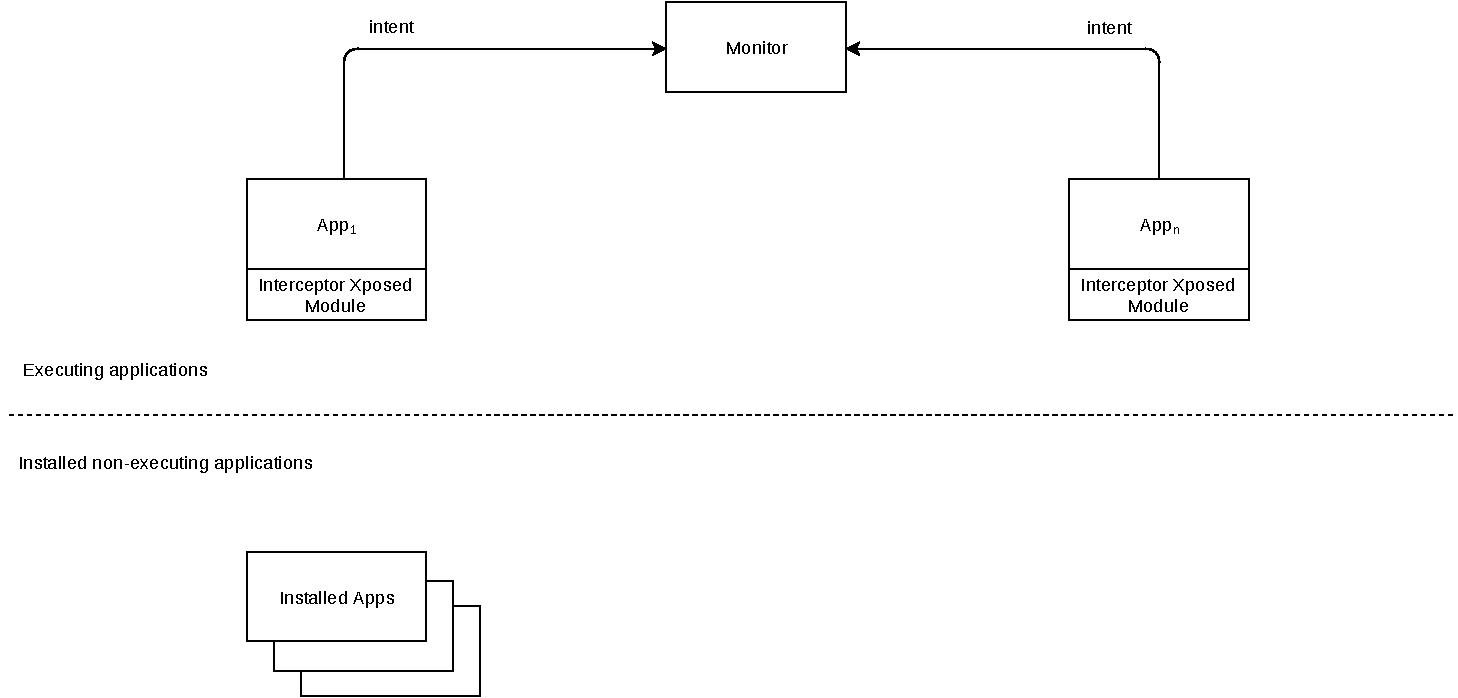
\includegraphics[width=\textwidth]{graphics/HighLevelArchitecture.pdf}
  \caption{High Level Architecture Diagram}
  \label{fig:highLevelArchitectureDiagram}
\end{figure}

\FloatBarrier

\section{Interceptor}
\label{sec:Interceptor}

The first part of the monitoring system is an Xposed module called the interceptor.  Figure \ref{fig:interceptorClassDiagram} below shows the structure.  The interceptor contains callback classes derived from XC\_MethodHook that Xposed hooks to interesting operating system methods.  Whenever a hooked method is called, the callback is invoked first, then the O/S method will be allowed to continue as usual.

The Xposed framework injects the callbacks into every process, therefore intercepted O/S calls will be from every process.  In order to recognise collusion between different applications, we must gather the details of the calls into a single trace.  Callbacks do this by capturing details of the method calls and notifying a single monitor process via an Android intent.

It is relevant now to mention a quirk that leads to a hazard we must avoid.  Xposed will inform the interceptor of its own attempt to send an intent to the monitor.  In addition, the monitor process will have the interceptor module injected into it.\footnote{This technicality is omitted from figure \ref{fig:highLevelArchitectureDiagram}.}  If the monitor system reports on its own activity, we hit the halting problem.  Of course, the interceptor knows the intent channel designated for communication to the monitor, so it ignores communication over that intent. 

Figure \ref{fig:interceptorClassDiagram} below shows five classes derived from XC\_MethodHook, one for each of the methods of interest identified in section \ref{sec:OSMethodsOfInterest}.  The MethodHooks class implements IXposedHookLoadPackage.handleLoadPackage() that is invoked whenever any process requires a package to be loaded.  If the package contains one of the operating system methods we are interested in, then the corresponding XC\_MethodHook class will be created and registered with Xposed.  Then, whenever the host process calls the interesting operating system method, beforeHookedMethod() will be called on the XC\_MethodHook class, and the interceptor will notify the monitor.

\begin{figure}[h]
  \centering
  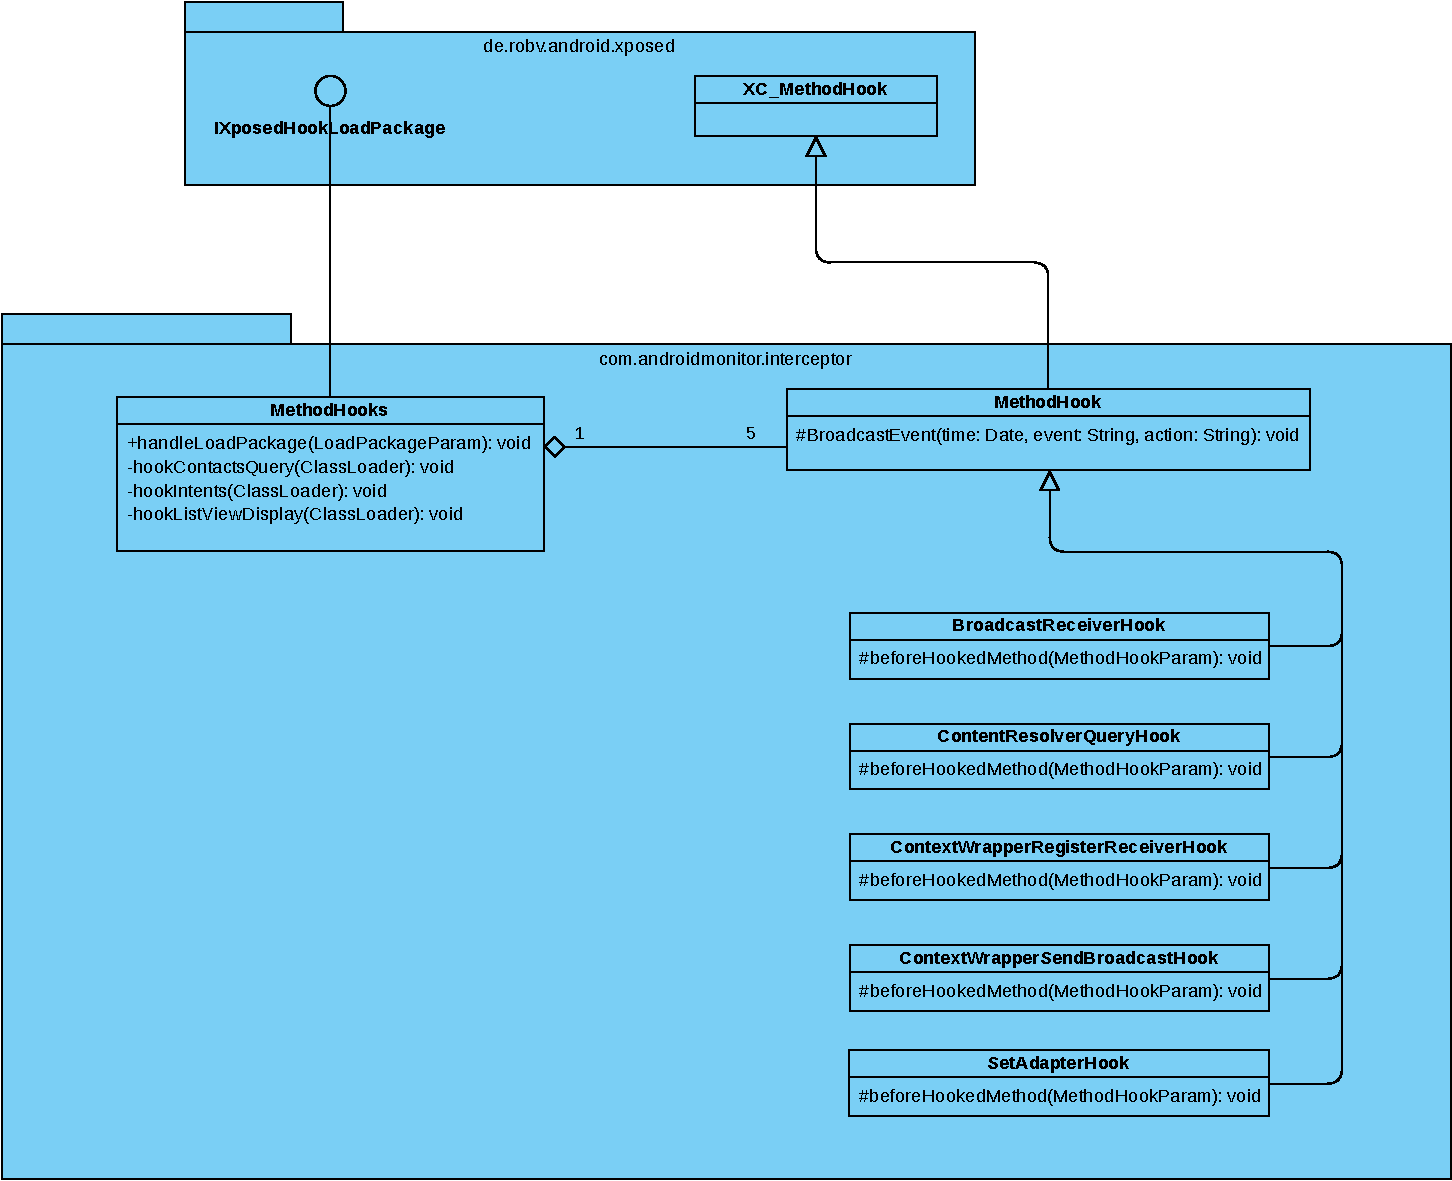
\includegraphics[width=\textwidth]{graphics/InterceptorClassDiagram.pdf}
  \caption{Interceptor Class Diagram}
  \label{fig:interceptorClassDiagram}
\end{figure}

\section{Monitor}
\label{sec:Monitor}

The second half of the system is the monitor.  The monitor receives intents from the interceptor, the details of the O/S call get extracted, put into an event, then passed to an instance of the \RH\ algorithm.  The event gets evaluated to determine if the formula is satisfied and if so, the monitor alerts the user that some malicious activity may have taken place.  The monitor could evaluate different formulae simultaneously by constructing multiple algorithm instances, one for each formula.  For now, we only evaluate the collusion formula.

\section{Benefits}
\label{sec:Benefits}

There is an added advantage to separating activity reporting from monitoring.  The intensive work for the developer is in evaluating the trace for the satisfaction of LTL formulae.  Whereas the reporting of activities is relatively straightforward.  Furthermore, once interesting O/S methods have been identified, and there is code implemented to intercept them, that code requires little maintenance.  This is a great benefit because the interceptor becomes the only part of the system dependent on the Xposed framework.

Development with this framework has proved awkward because of its nature.  The Xposed module code gets injected into the Android zygote process on boot-up of Android.  For a module to take effect, it is necessary to reboot the device after the module gets installed.  Alterations to the module require the previous version to be uninstalled, the new version installed, and the device rebooted.  Not only does this slow the development cycle, but there are two important consequences:  Any faults in an Xposed module can result in Android failing to boot.  It is then impossible to remove the Xposed module because it can only be uninstalled using an administration tool launched within Android.  If Android does not boot, then the administration tool cannot be used to uninstall the faulty Xposed module.  The device is 'bricked'.

Experience has shown that developing on a virtual Android device and keeping a backup of it with all necessary development tools pre-installed is very prudent.  Faulty Xposed modules have also proved impossible to debug using standard debugging tools because the code begins executing on boot-up of Android rather than being launched once Android is running.  It is necessary to attach the debug tool to running processes, but this has been unsuccessful so far.  The upshot is that debugging tools that allow the developer to stop execution at a breakpoint within the code, trace through the code and inspect memory are unusable.  The risk of bricking the device during development makes all but the simplest code infeasible as an Xposed module.

Thankfully, if the Xposed module only intercepts interesting methods, then it is kept simple.  Once the module is complete, it does not require maintenance so development cycles are kept rapid.  It follows that the complex work falls into the monitor half of the system, where it is easier to debug and cannot render the device unusable.  We describe the structure of the monitor in later chapters \ref{chap:Runtime Verification with the Rosu-Havelund Algorithm} and \ref{chap:Reverse Rosu-Havelund Algorithm}.

\chapter{Runtime Verification with the \RH\ Algorithm}
\label{chap:Runtime Verification with the Rosu-Havelund Algorithm}

We will now investigate the suitability of the \RH\ algorithm for runtime verification in realtime using a monitor.  We start by performing a complexity analysis in section \ref{sec:ComplexityAnalysis} that indicates the algorithm appears to be too time-consuming for real-world use when applied.  Then, we confirm those suspicions by performing a practical performance analysis on an implementation of the algorithm.  The implementation is described in section \ref{sec:RosuHavelundImplementation}, followed by some tests in section \ref{sec:FunctionalTestingRosuHavelund} to ensure the correct functioning of the implementation.  In section \ref{sec:PracticalPerformanceAnalysisOfRosuHavelund} a practical analysis is conducted to ascertain the performance over increasing workload.  We finish by explaining the weakness in the algorithm in section \ref{sec:ScalabilityOfRosuHavelund}.

\section{Complexity Analysis}
\label{sec:ComplexityAnalysis}

The computational cost of the \RH\ algorithm is composed of memory cost and execution cost for the initialisation and evaluation phases of the algorithm.  It depends upon the size of the formula being evaluated and the length of the trace evaluated over.  The size of the formula is the number of subformulae $ | \varphi | $ and the trace length is the number of trace events $ | t | $.

The memory and execution cost of the initialisation phase is simply the cost of constructing the \textit{now} and \textit{next} registers. The memory required for each register is equal to the size of $ \varphi $, and the execution cost increases linearly with the size of $ \varphi $.  Both memory and execution costs of the initialisation phase are O($ | \varphi | $).

Evaluation of the formula over a trace takes place in a loop where each iteration evaluates the formula over a different trace event until the evaluation has covered all events.  It is imperative that every event in a trace is considered when evaluating a formula because the always operator requires the left operand is satisfied for all trace events.  Each of the individual trace entries gets evaluated against every subformula in the \textit{now} register.  Thus the execution cost rises linearly with the size of the formula multiplied by the length of the trace. It is O($ | t | * | \varphi | $).

The memory cost of the evaluation phase is simply the cost of storing the trace.  Therefore it rises linearly with the length of the trace, i.e.,\ the complexity is O($ | t | $).

However, this describes only the static cost of the evaluation phase; the cost of evaluating the formula once over a trace of finite length.  But when the algorithm gets applied in real-world situations, the system being monitored can run for an indefinite period.  Thus any number of events can occur during the execution life of the algorithm.  When new events occur, they get added to the trace, and the formula must be re-evaluated over the new trace.  The reader should draw their attention now to a significant detail regarding the algorithm.  The loop that iterates through the trace does so in reverse order.  It evaluates the formula over the latest trace entry first and continues until the earliest entry.  Meaning, to correctly evaluate an LTL formula, which may include the always operator, entries can never be removed from the trace.  This poses two fatal problems:  Firstly, the dynamic memory requirements increase indefinitely because the trace grows, albeit linearly, in length and entries can never be removed.  Secondly, the dynamic execution cost increases indefinitely as the trace grows.  But unlike the memory requirement, the dynamic execution cost grows at a far greater rate.  For example, after a single event has occurred, the formula is evaluated over a trace of length 1.  When a second event occurs the formula is re-evaluated over a trace of length 2.  After the next event, the evaluation is over a trace of length 3, and so on.  To illustrate the point, when ten events occur in succession the formula gets evaluated 1+2+3+4 ... 10, a total of 55 times.

The general formula describing the number of evaluations is $ n(n+1)/2 $ where $ n = | t |$, the length of the trace.  In application, the dynamic execution cost of the algorithm is $$O((n(n+1)/2 * |\varphi |) = O((n^2+n)/2 * | \varphi |) = O(n^2 * |\varphi |) = O(| t |^2 * |\varphi |)$$

Therefore when events occur in succession, it requires $ | t |^2 * | \varphi | $ iterations of the evaluation phase to evaluate the formula over the trace.  Such an algorithm has quadratic complexity and will quickly become too time-consuming to be useful.

\section{Implementation}
\label{sec:RosuHavelundImplementation}

Before implementing the algorithm, we were conscious that further investigation into performance improvements were necessary.  With this in mind, the implementation follows an ad-hoc structure where the intention is simply to have a functioning implementation that is true to the design of the algorithm.  Given that further development was likely, this gave us the opportunity to become familiar with the general implementation challenges presented during the standard implementation.  We intended to leave more elegant solutions to a second development cycle where the algorithm would be improved.  In our experience, a two-cycle development approach is welcome when developing anything new because the challenges are understood better after the first cycle.\\

\noindent The algorithm was developed in Java using the Eclipse IDE.  Download it from here:\\
\indent \url{https://www.eclipse.org/downloads/}\\
\\
Appendix \ref{app:RHCode} provides links to the implementation code. 

\subsection{Syntax of Implemented LTL}

For convenience, our implementation of \RH\ allows LTL formulae to be written as free-text strings and parsed during the initialisation phase of the algorithm.  The description of LTL in chapter \ref{chap:Linear Temporal Logic} uses characters that are not available on a typical computer keyboard.  For this reason, we chose alternative characters to represent the LTL operators that are based, where possible, on the characters used in the familiar C language.  Table \ref{tab:AlternativeLTLOperators} gives the translations and includes future and past temporal operators.

\begin{center}
\begin{tabular}{c|c|c} 
Operator  & LTL & Implementation\\
\hline
AND & $ \land $ & \&\& \\
OR & $ \lor $ & $ \mid \mid $ \\
IMPLIES & $ \rightarrow $ & \texttt{=>} \\
NOT & $ \neg $ & ! \\
ALWAYS & $ \LTLalways $ & \texttt{[]} \\
EVENTUALLY & $ \LTLeventually $ & \texttt{<>} \\
NEXT & $ \LTLnext $ & N \\
UNTIL & $ U $ & U \\
ALWAYSBEEN & $ \LTLalwaysbeen $ & \texttt{[-]} \\
ONCE & $ \LTLonce $ & \texttt{<->} \\
PREVIOUS & $ \LTLprevious $ & P \\
SINCE & $ S $ & S \\
\hline
\end{tabular}
\captionof{table}{LTL Operator Translations\label{tab:AlternativeLTLOperators}}
\end{center}

The parser also requires formulae to be fully parenthesized to delineate subformula.  When the parser is presented with a formula, it first strips the outer parenthesis off the string, then searches the string until it encounters an operator.  The number of open parenthesis found before the operator that do not have a matching close parenthesis get counted.  If there count is zero, then the operator is outside all open parenthesis and it is taken as being the root operator of that subformula.  The operands are taken as being the strings to the left and right of the operator, or just the right in the case of a unary operator.  Each operand becomes a subformula and the process repeats until the operands are reduced to literals, at which point parsing is complete.

\begin{myEx} The example formula we have been working with so far is:\\

$ \LTLalways((p \,U q) \rightarrow \LTLeventually(q \rightarrow \LTLnext r)) $\\

When written using the implementation syntax the formula becomes:

([]((p U q) $=>$ (\texttt{<>}(q $=>$ (N(r))))))

\qed
\end{myEx}

\section{Functional Testing of \RH}
\label{sec:FunctionalTestingRosuHavelund}

We aim to answer two questions with our test program, whether the implementation functions correctly and how the algorithm performs with traces of increasing length.  In this section we describe a series of functional tests that confirm the correct implementation of the algorithm.  We present how test cases were chosen and executed.  The tests are documented in appendix \ref{app:RHFunctionalTestCases} and detailed results of each test are documented in appendix \ref{app:RHFunctionalTestResults}.

\subsection{Test Case Selection}
\label{subsec:FunctionalTestCaseSelection}

Appendix \ref{app:RHFunctionalTestCases} describes a series of functional tests that will give us case-coverage of every LTL operator we implement.  We use the following testing hypotheses:

\begin{enumerate}
\item If the algorithm is correct for an alphabet of size 3 or larger, then it will be correct for any alphabet.  Thus we choose an alphabet including a, b and c.

\item We assume that an LTL operator works in the same way at any depth in the formula.  Thus it will suffice to test each operator in isolation, i.e., it is enough to provide one test suit for each operator where we test for all outcomes.
\end{enumerate}

Each table presents test cases for a specific operator.  A test case has two inputs; a formula chosen to isolate a specific operator, and a finite trace.  The complete series of test cases are chosen to produce every true and false result for each operator.  We decide what result we expect to get for each test case by evaluating the formula over the trace by hand, applying the semantics from chapter \ref{chap:Linear Temporal Logic}, and noting whether that trace satisfies the formula.  One such test suit is reproduced in table \ref{tab:NotOperatorFunctionalTests}.

\begin{table}[h!]
	\centering
	\begin{tabular}{l r}
		\begin{tabular}{c|c} 
		Operator & Formula\\
		\hline
		NOT & $ (!a) $\\
		\hline
		Trace & Expected Result \\
		\hline\hline
		$ \langle \rangle $ & True \\
		$ \langle a \rangle $ & False \\
		$ \langle b \rangle $ & True \\
		\hline
		\end{tabular}
	\end{tabular}
	\caption{NOT Operator Functional Tests}
	\label{tab:NotOperatorFunctionalTests}
\end{table}

We draw attention to the operators AND and IMPLIES.  They can only be successfully tested in combination with another operator because a trace event can never be one literal value and another.  Therefore, the AND and IMPLIES tests expect one operand to be an event of a particular value, and the other operand to be an event elsewhere in the trace of a different value.  Otherwise, the test always fails.

\subsection{Test Execution}
\label{subsec:FunctionalTestExecution}

The functional tests were run by a test harness that writes the results to the standard output.   It accepts a trace and a formula as inputs, constructs an instance of the \RH\ implementation, then evaluates the formula over the trace.  The test harness is a simple command line executable written in Java as an Eclipse project and links to the source code are in appendix \ref{app:RHCode}.

\subsection{Test Results}
\label{subsec:FunctionalTestResult}

A total of 49 tests were performed, the results of which are in appendix \ref{app:RHFunctionalTestResults}.  The results show the satisfaction of the formula after every prefix of the trace.  The NOT operator results reproduced below, show three tests cases with different traces and the actual result of each.\\

\indent	Formula:\\
\indent	(!a)\\
\\
\indent	Subformulae:\\
\indent	!a\\
\indent	a\\
\\
\indent	Running Trace: \textless \textgreater\\
\indent	Prefix: \textless \textgreater\\
\indent	Formula satisfied = true\\
\\
\indent	Actual Result = true\\
\\
\indent	Running Trace: \textless a\textgreater\\
\indent	Prefix: \textless a\textgreater\\
\indent	Formula satisfied = false\\
\\
\indent	Actual Result = false\\
\\
\indent	Running Trace: \textless b\textgreater\\
\indent	Prefix: \textless b\textgreater\\
\indent	Formula satisfied = true\\
\\
\indent	Actual Result = true\\

\noindent Naturally, the development cycle continued until the actual result of all 49 test cases equalled the expected result from appendix \ref{app:RHFunctionalTestCases} and we were able to conclude that all tests passed.

\section{Practical Performance Analysis of the \RH\ Algorithm}
\label{sec:PracticalPerformanceAnalysisOfRosuHavelund}

With functional testing of the implementation complete, we now intend to confirm the result of the complexity analysis from section \ref{sec:ComplexityAnalysis}. We conducted practical performance tests of the algorithm to study the relationship between the length of the trace and the time required to evaluate it.  Each test increased the trace length and recorded the time taken to evaluate the trace.

\subsection{Test Environment}
\label{subsec:RHPracticalPerformanceAnalysisEnvironment}

We took the opportunity to design a test environment that closely resembles the architecture described in figure \ref{fig:highLevelArchitectureDiagram}.  Our implementation of the \RH\ algorithm runs inside our monitor application.  The monitor receives events from the interceptor via the Android intent inter-process communication system.  The events originate from two applications called the reader and publisher that can perform a collusion attack at will.  Callum Dicker originally developed the apps during his earlier dissertation on collusion \cite{Dicker}, and we enhanced them to aid our testing.  Figure \ref{fig:readerPublisherGUI} shows the reader and publisher user interfaces.  All tests were run on a virtual Android device.

\begin{figure}[h!]
	\begin{subfigure}[h]{0.5\textwidth}
	\centering
	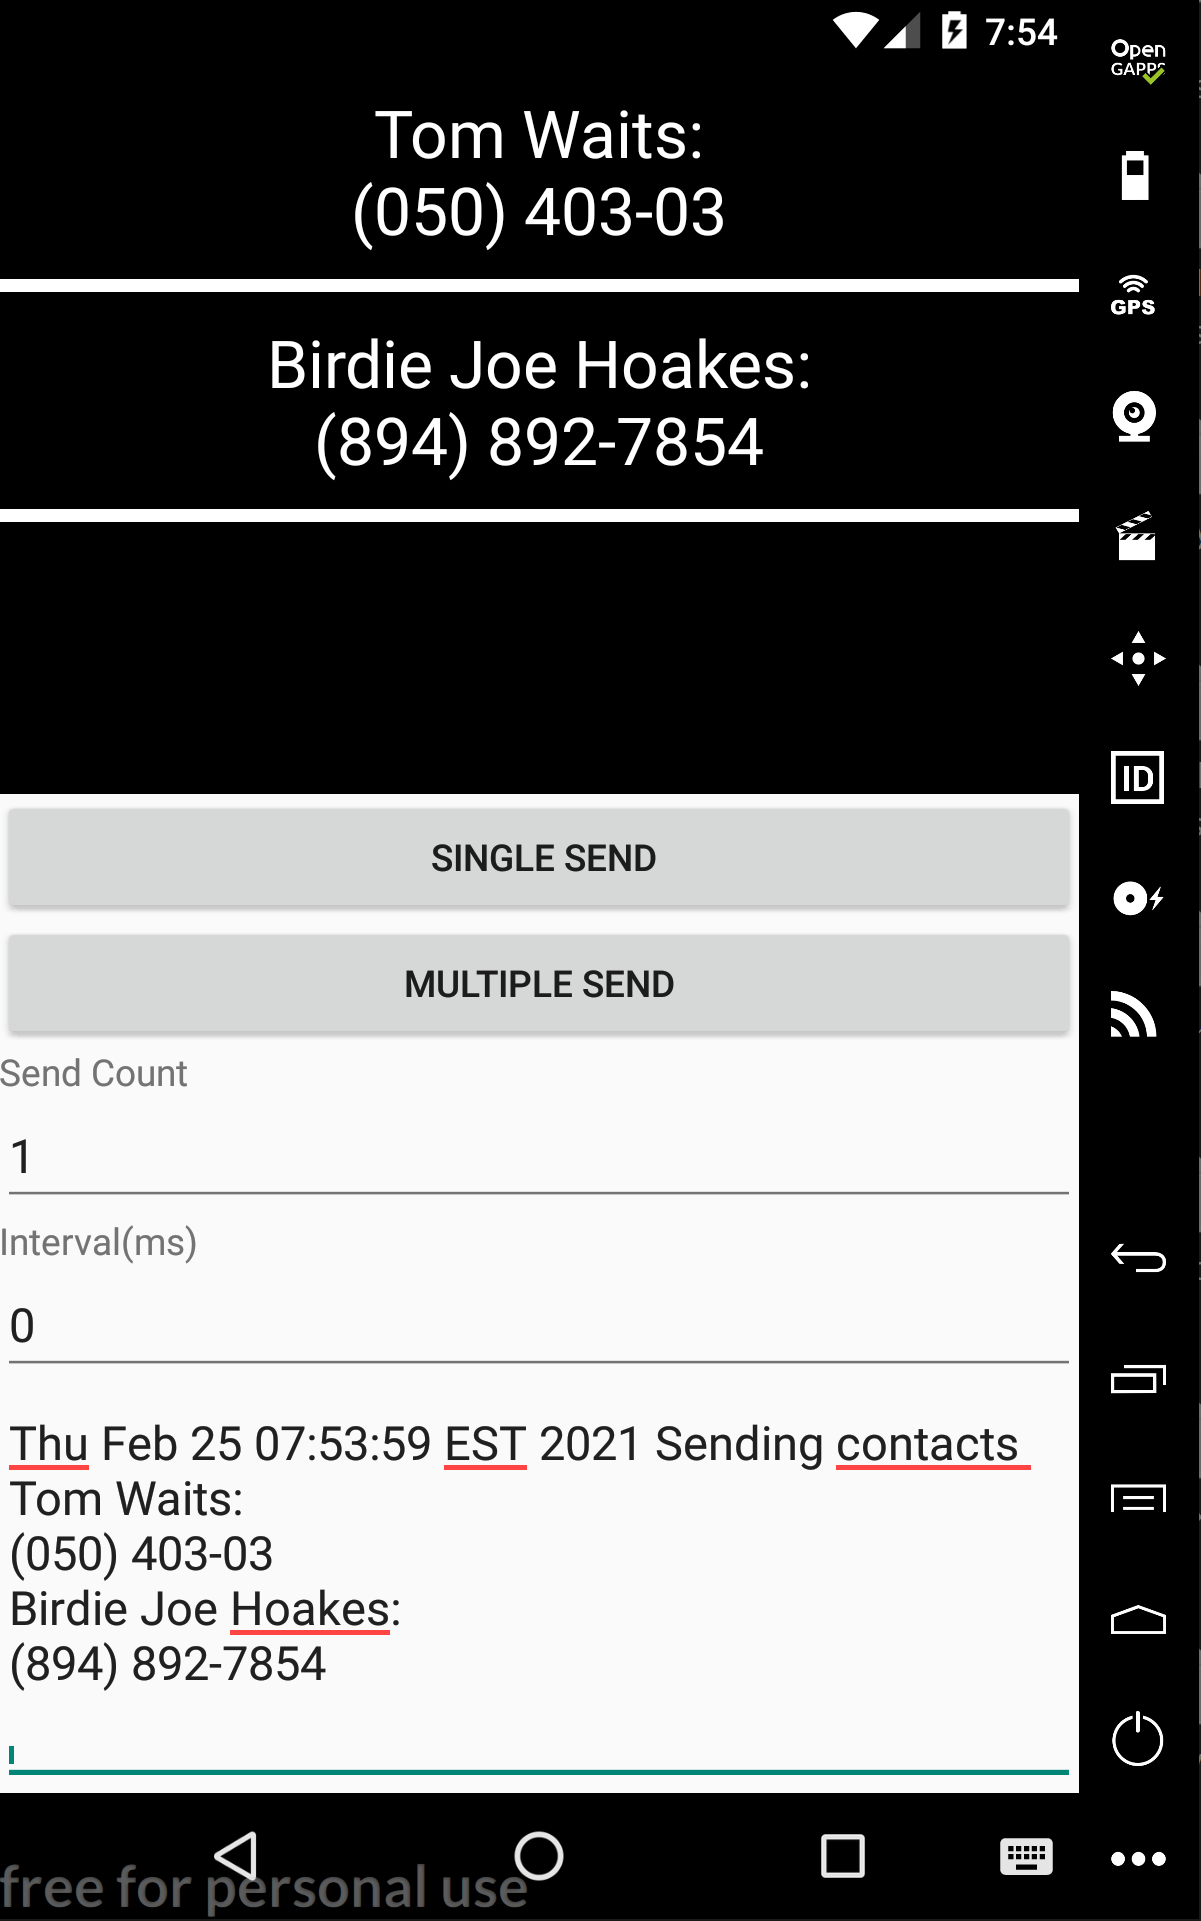
\includegraphics[height=0.5\textheight]{graphics/Reader}
	\caption{Reader}
	\label{fig:readerGUI}
	\end{subfigure}
\hfill	
	\begin{subfigure}[h]{0.5\textwidth}
	\centering
	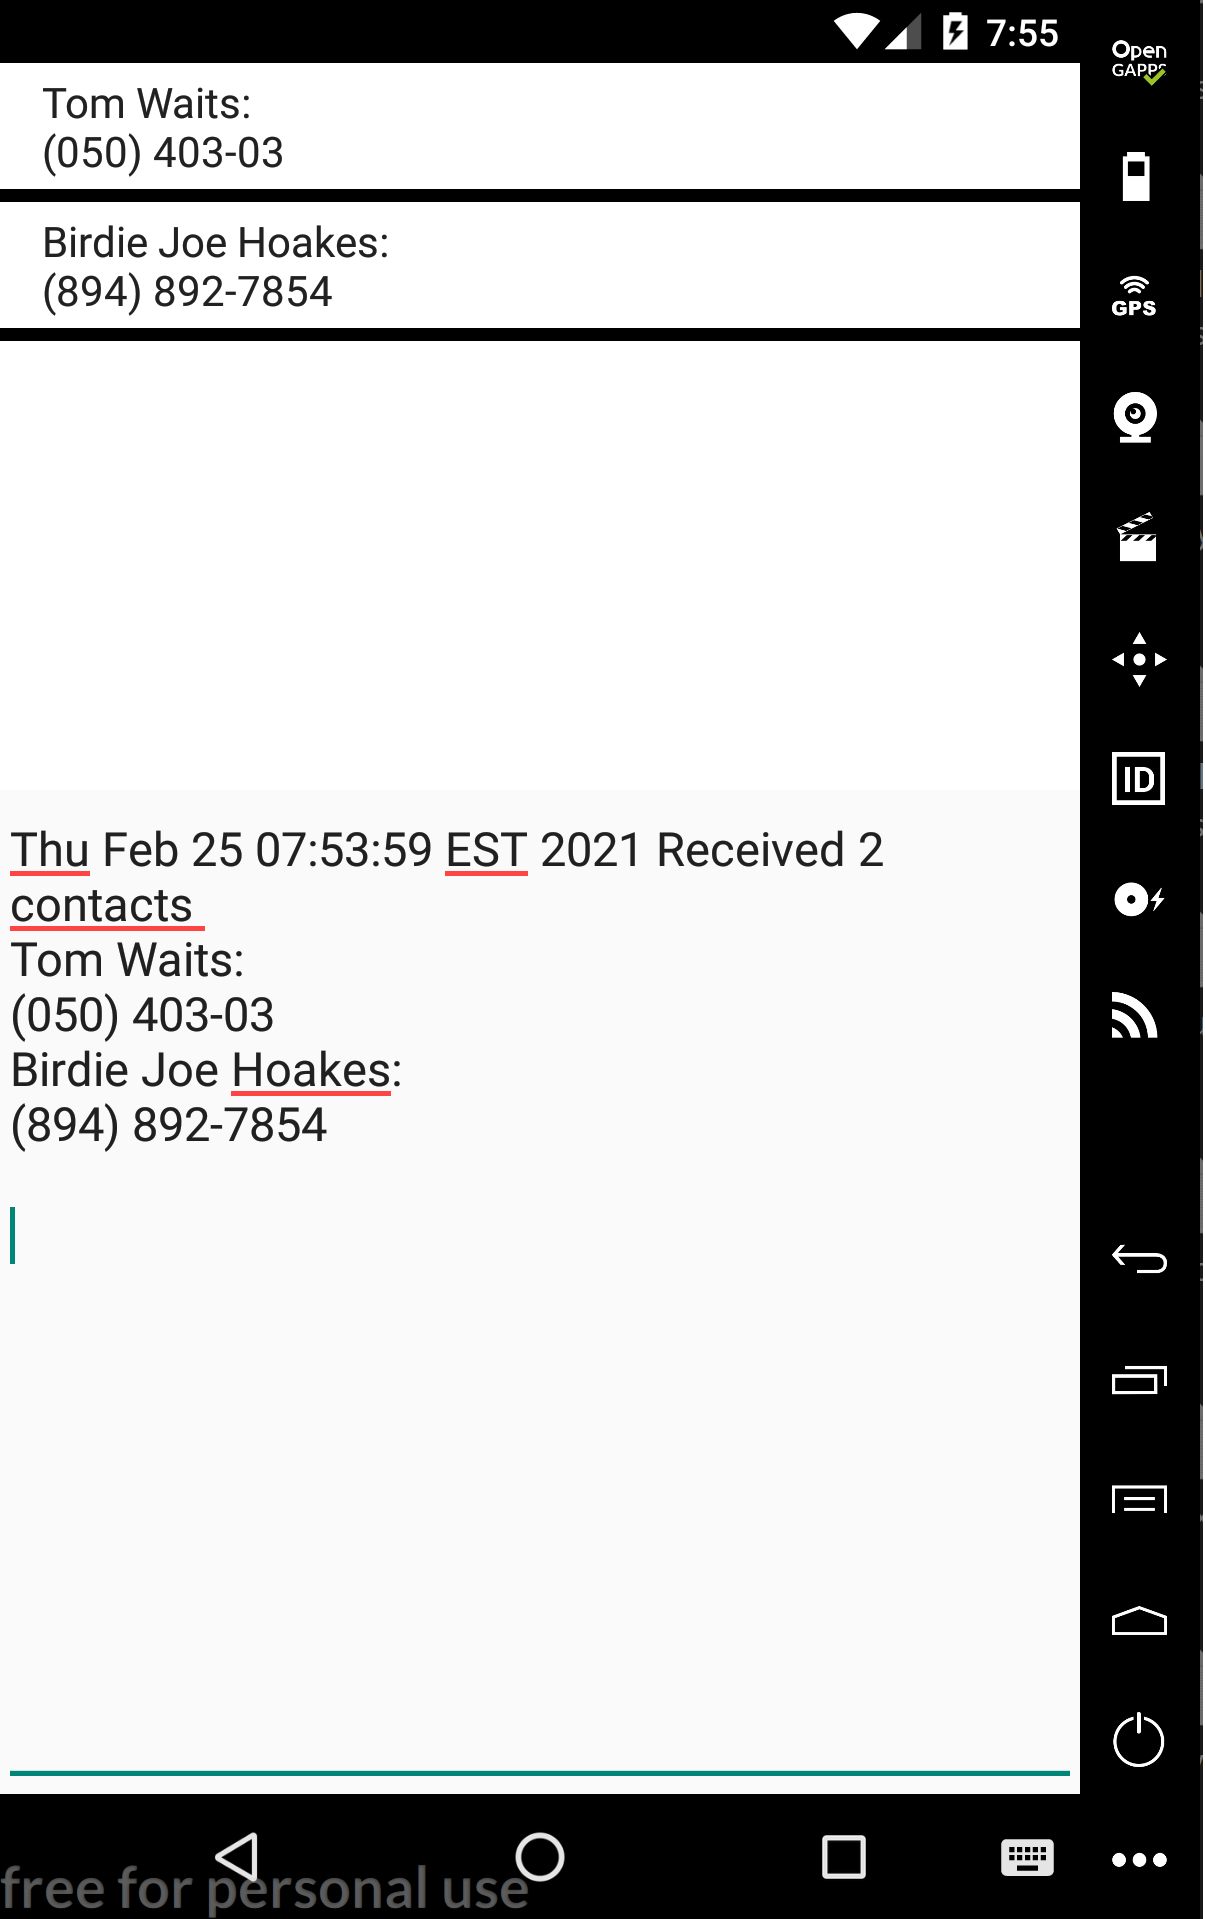
\includegraphics[height=0.5\textheight]{graphics/Publisher}
	\caption{Publisher}
	\label{fig:publisherGUI}
	\end{subfigure}
\caption{Reader \& Publisher GUI}
\label{fig:readerPublisherGUI}
\end{figure}

The reader application reads the contacts list on the Android device and sends it to the publisher via an intent.  The publisher displays what it receives on the screen. The two applications do this using the O/S methods we are interested in monitoring from section \ref{sec:OSMethodsOfInterest}.  The interceptor module that is embedded into the reader and publisher at runtime, recognises when they call the methods of interest and notifies the monitor via intents.  The monitor hosts the very same implementation of the \RH\ algorithm used in the functional testing, we simply placed that code into the monitor and added the ability to receive intents from the interceptor.

All components of this test environment were developed in Java using the Android Studio IDE.  Links to the source code for the reader and publisher apps, the interceptor and the standard \RH\ monitor are in appendices \ref{app:PerformanceTestCode}, \ref{app:InterceptorCode} and \ref{app:StandardRHMonitorCode} respectively.

\newpage

\subsection{Test Execution}
\label{subsec:PracticalPerformanceAnalysisExecution}

To understand the relationship between evaluation duration and trace length, we ran a series of ten tests where the trace length increased for each test.  The first test performed ten collusion attacks, and each subsequent test increased the number of attacks by ten until the last test performed a total of 100 attacks.  To stage multiple collusion attacks, we enhanced the reader app to read the contacts list multiple times, in a tight loop.

We used the Android Studio Profiler tool to measure the time required to evaluate a trace.  The profiler is a debug tool that works by launching the process under test on the test device and attaching to that process.  It can then measure the hardware usage of the process.  Figure \ref{fig:androidProfiler} is a screenshot of the profiler tool in operation on the monitor.  The top graph, shaded green, shows the CPU usage over time.  Memory usage over time is shown in the lower graph, shaded blue.  

To run a test, we launched the reader and publisher apps on the virtual Android device and used the profiler to launch the monitor on the virtual device.  We started the test by clicking the Multiple Send button on the reader, then watched the CPU usage of the monitor process.  The CPU usage would rise when the monitor received events from reader and publisher apps and then return to the idle level when the evaluation was complete.

The time required to evaluate the entire trace was measured as the difference between when CPU usage ramped up and when CPU usage returned to the idle level.

\begin{figure}[h!]
\centering
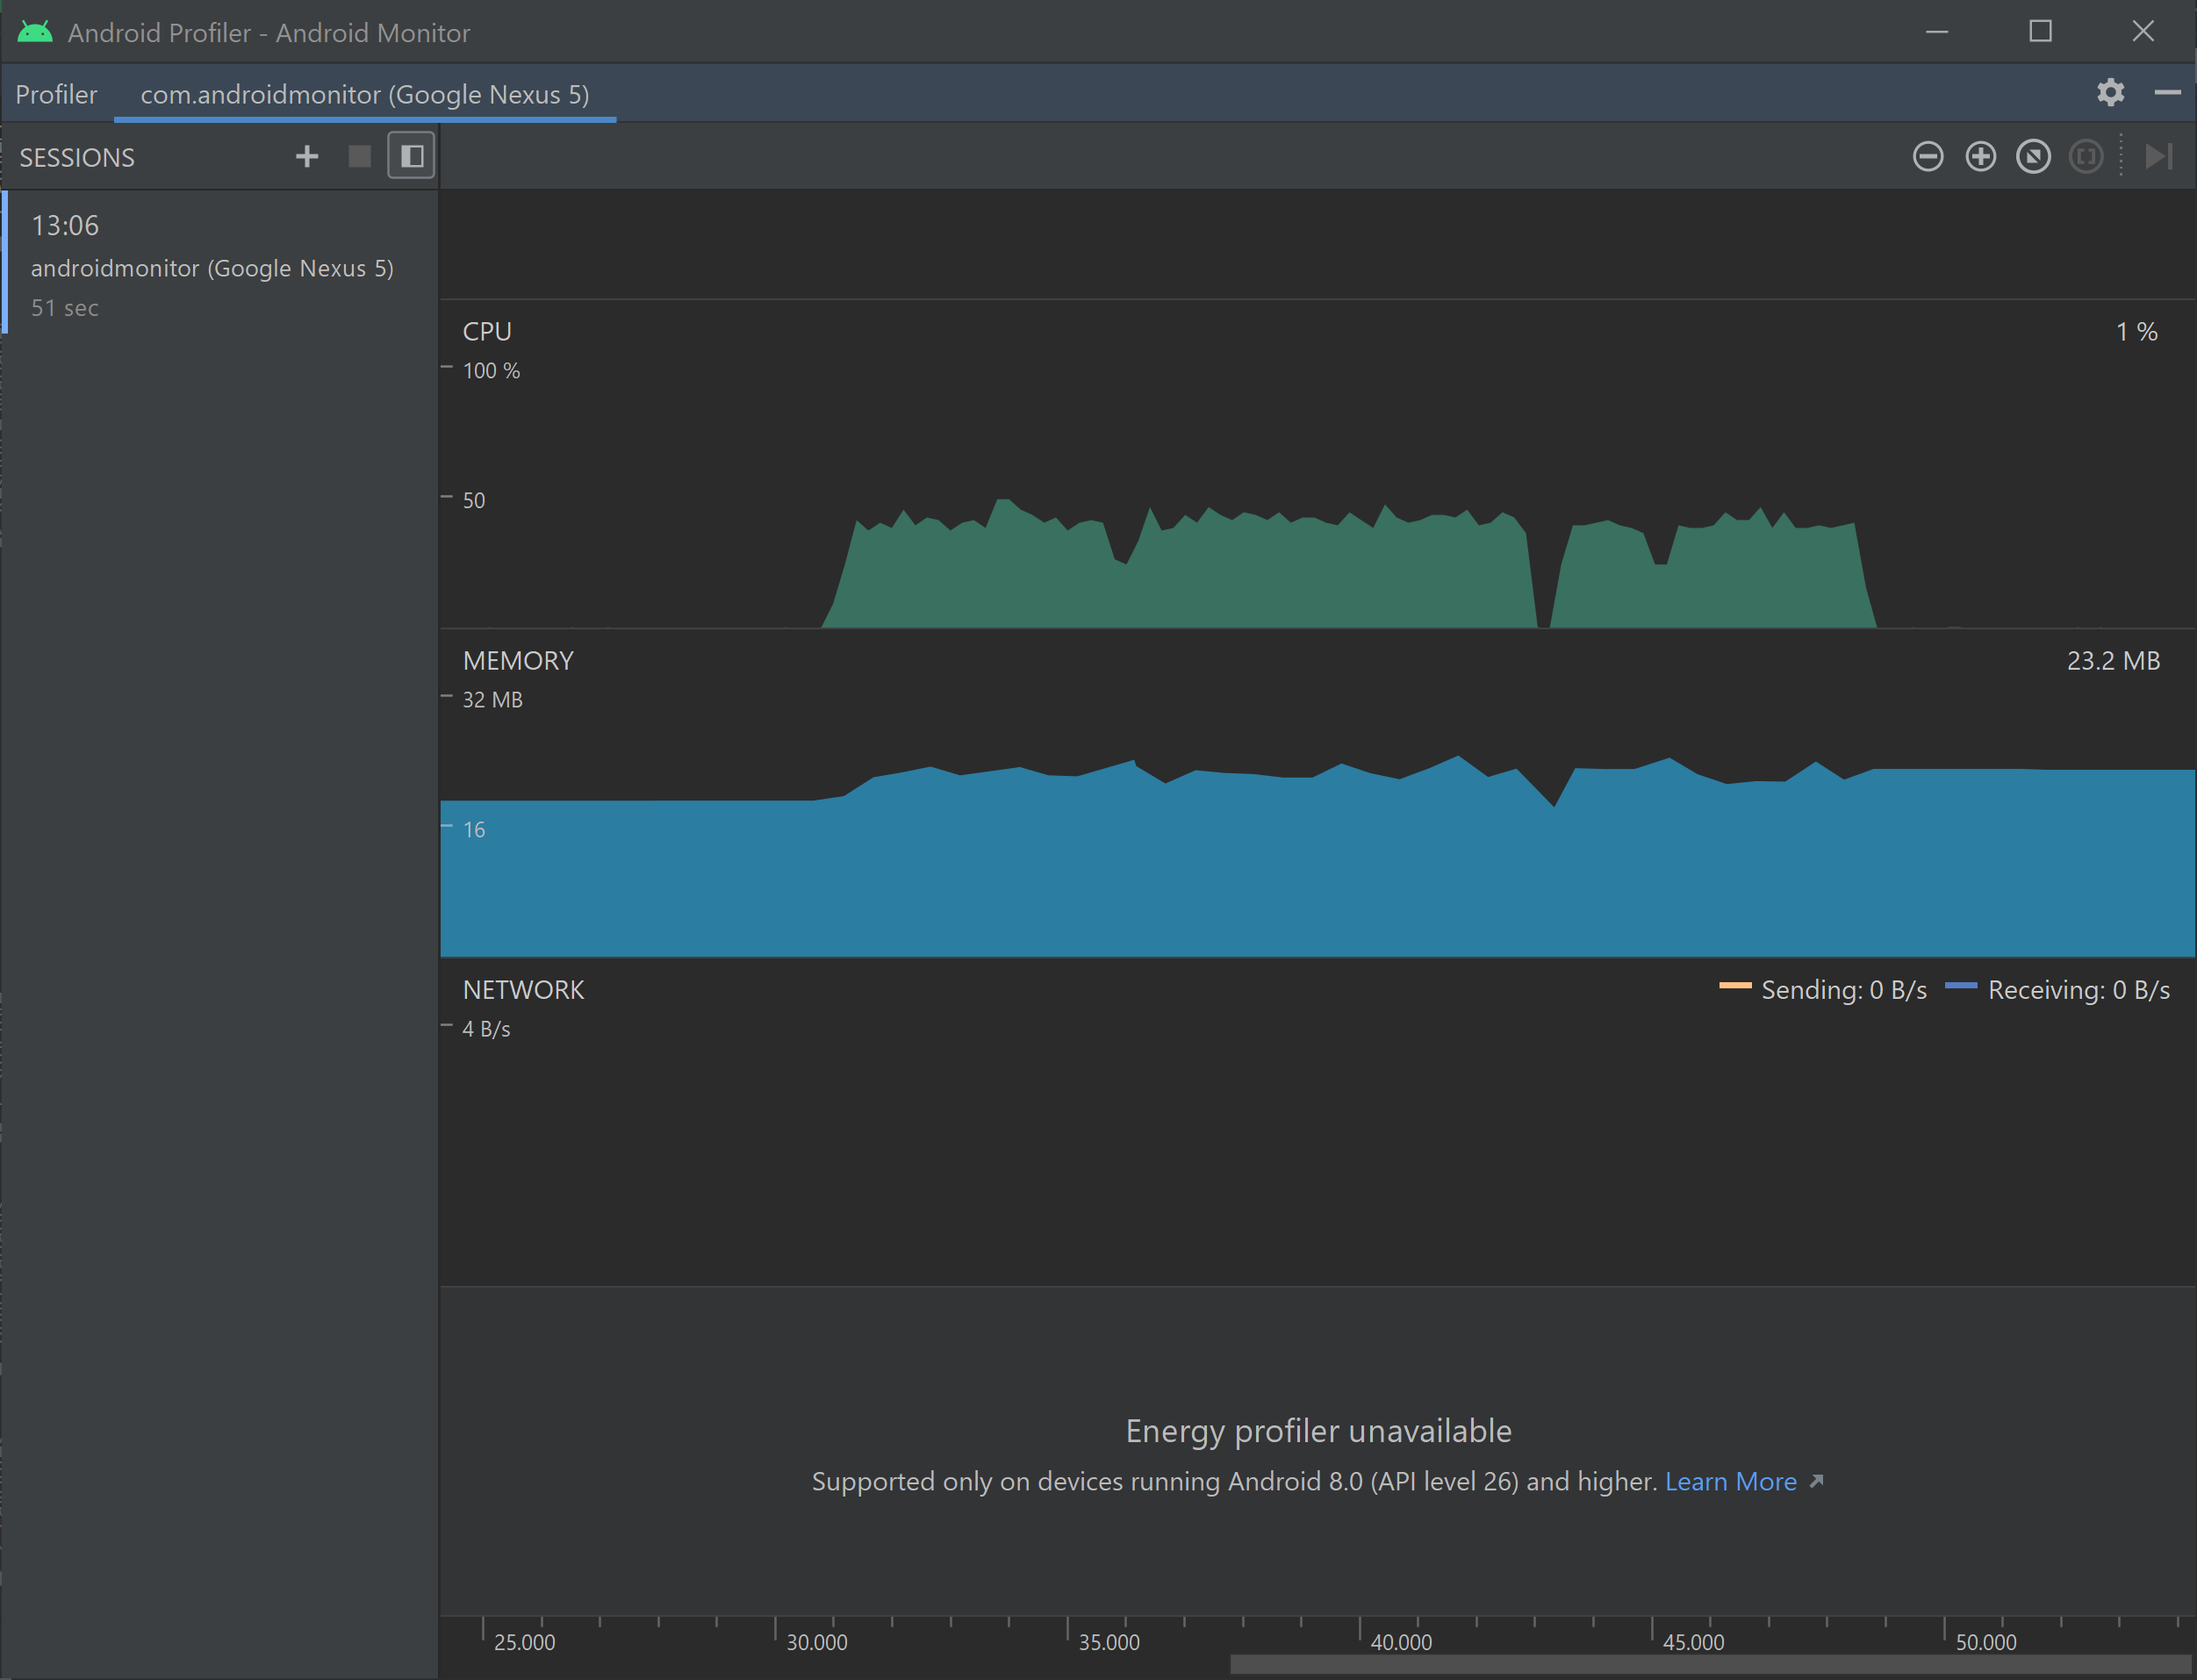
\includegraphics[width=\textwidth]{graphics/AndroidStudioProfiler3}
\caption{Profiler Tool}
\label{fig:androidProfiler}
\end{figure}

\newpage

\subsection{Test Results}
\label{subsec:PracticalPerformanceAnalysisResults}

Table \ref{tab:StandardRHExecutionTimes} shows the number of seconds elapsed when evaluating traces of increasing length.  Each row in the table is the result of a test where the trace length is greater than that of the previous test.

\begin{table}[h!]
	\centering
	\captionsetup{width=0.6\linewidth, justification=centering}
	\begin{tabular}{r|r} 
	Trace Length  & Duration\\
	(collusion sequences) & (seconds)\\
	\hline
	10 & 17\\
	20 & 72\\
	30 & 145\\
	40 & 203\\
	50 & 326\\
	60 & 462\\
	70 & 692\\
	80 & 941\\
	90 & 1198\\
	100 & 1449\\
	\hline
	\end{tabular}
	\caption{Duration of the \RH\ Algorithm Evaluating Traces of Increasing Length}
	\label{tab:StandardRHExecutionTimes}
\end{table}

\section{Scalability and Performance of the \RH\ Algorithm}
\label{sec:ScalabilityOfRosuHavelund}

Graph \ref{tab:StandardRHEvaluationDuration}, below, presents the actual test results alongside the theorised duration.  The blue curve plots the measured duration, and the red curve plots the theorised number of computational steps.  We can see that while the two curves are not precisely the same, there is a correlation between the measured duration and the theorised number of computational steps.  The measured duration curve confirms our conjecture from section \ref{sec:ComplexityAnalysis} that the time required to evaluate a trace rises quadratically with trace length.

\begin{figure}[h!]
	\centering
	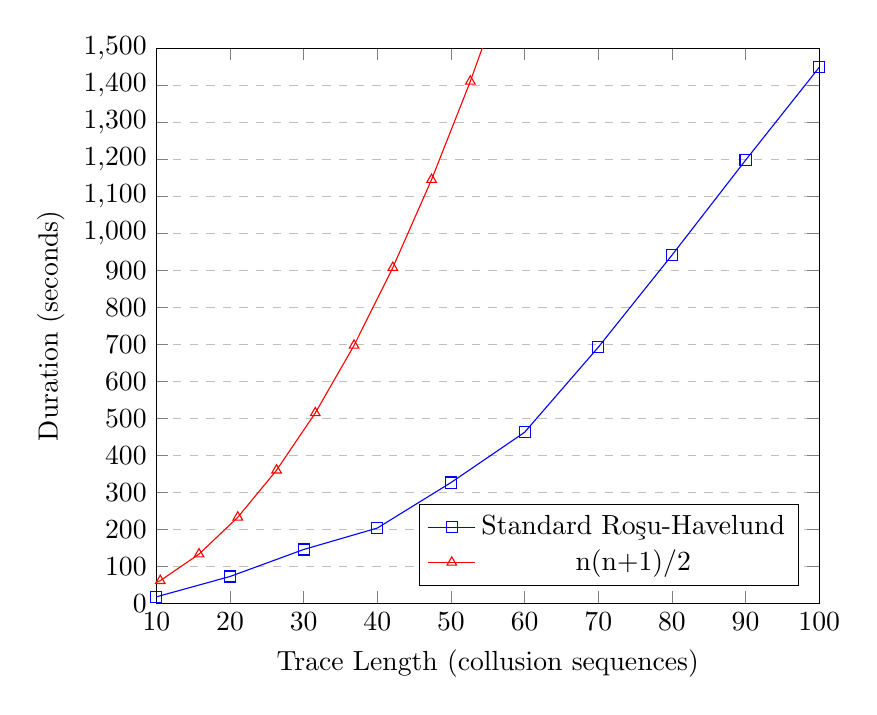
\begin{tikzpicture}
	\begin{axis}[
	    xlabel={Trace Length (collusion sequences)},
	    ylabel={Duration (seconds)},
	    xmin=10, xmax=100,
	    ymin=0, ymax=1500,
	    xtick={10,20,30,40,50,60,70,80,90,100},
	    ytick={0,100,200,300,400,500,600,700,800,900,1000,1100,1200,1300,1400,1500},
	    legend pos=south east,
	    ymajorgrids=true,
	    grid style=dashed,
	]
	
	\addplot[
	    color=blue,
	    mark=square,
	    ]
	    coordinates {
	    (10,17)(20,72)(30,145)(40,203)(50,326)(60,462)(70,692)(80,941)(90,1198)(100,1449)
	    };
	    \addlegendentry{Standard \RH}
	    
	\addplot[
	    domain=0:100, 
	    samples=20, 
	    color=red,
	    mark=triangle,
	    ]
	    {(x * (x+1)) / 2};
	    \addlegendentry{n(n+1)/2}    
	\end{axis}
	\end{tikzpicture}
	\caption{Dependency Between Trace Length and Evaluation Duration}
	\label{tab:StandardRHEvaluationDuration}
\end{figure}

When applied to realtime monitoring, the monitor should react to events as they occur and compute the outcome before the next event arises.  Otherwise, the monitor will become overwhelmed and never finish evaluating:\\

\indent Let $e_1$ and $e_2$ be two consecutive events.\\
\indent Lets denote the time interval between $e_1$ and $e_2$ with $I$.\\
\indent Lets call the computation time of the monitor $T$.\\
\indent Then we require from the monitor that $T \textless I$.\\
\\
With the \RH\ algorithm $T$ grows with the length of the trace. The trace will be recorded for an indefinite period, therefore the runtime of the \RH\ algorithm is unbounded and will eventually exceed any $I$.  For a technical system, it is realistic to have some expectation of the duration of $I$. That expectation is that there is no upper bound and the lower bound is in the order of milliseconds in the context of an operating system like Android. We estimate the minimum $I$ to be the interval between context switches plus the time to perform a context switch.

A solution to this problem might be to limit the length of the trace by removing the earliest event when a new event occurs.  But as $I$ is small, \RH\ will be limited to small traces.  And as we mentioned earlier in section \ref{subsec:ResettingTheMonitor}: If the length of the trace is limited, and the length of the attack sequence exceeds it, then the first act of the attack will have happened so far in the past that the event is no longer in the trace.  Therefore it becomes impossible to detect the attack.\\
\\
It is evident from these observations that the algorithm is not suitable for realtime monitoring.\\

%Deleting information comes at the price that monitoring is prone to miss attacks: An attack sequence comprises events corresponding to the actions of the attack.  The length of an attack sequence is unbounded, and to compound the problem, the trace may have unrelated events between the events of the attack sequence.\\
%
%\indent Let $e_n$ be the first event in an attack sequence, $e_m$ be the last event in the sequence and $n \leq m$.\\
%\indent Lets denote an attack sequence $e_n...e_m$ with $s$.\\
%\indent Lets call the trace $t$.\\
%\indent Then the monitor requires that $| s | \leq | t |$.\\
%\\
\chapter{\RRH\ Algorithm}
\label{chap:Reverse Rosu-Havelund Algorithm}

The reverse algorithm solves the shortcomings of the standard algorithm by changing the order in which the trace events are visited during evaluation.  The order is reversed to evaluate the trace from the earliest entry to the latest.  The effect of this is that when a new event occurs and the trace must be re-evaluated, that new evaluation always begins at the same event as the previous evaluation; the earliest event.

This is in contrast to the standard algorithm which visits the latest event first and moves backwards to the earliest event.  The problem is that the latest event is always different after a new event has occurred, so when evaluating a trace under the standard algorithm, that evaluation always begins from a new event.  This is a crucial detail because the standard algorithm involves the \textit{next} register.  The purpose of the \textit{next} register is to accumulate the evaluation result of each event in the trace as they are visited.  But at the moment when a new event occurs the result held in the \textit{next} register becomes invalid because it was determined before the new event happened.  Therefore, under the standard algorithm the \textit{next} register must be entirely redetermined every time a new event occurs, otherwise the final result of evaluating the trace will be incorrect.\\
\\
\section{Comparison Between Standard and Reverse Algorithms When Evaluating an Extending Trace}

To demonstrate the problem with the standard algorithm and the solution, we will compare the intermediate result of evaluating a trace that increases in length.  We will first use the standard, and then the reverse algorithm and show the intermediate result after each evaluation.  

\begin{myEx} Standard \RH\\
\\
\noindent
The \textit{next} register is defined as an intermediate result in a computational sequence that we wish to reuse between evaluations.\\
\\
\indent Let $t_1$ be a trace,\\
\indent as events occur $t_1$ is extended by one event,\\
\indent after the first event $t_1 =\ <e_1>$,\\
\indent after the second event $t_1 =\ <e_1, e_2>$,\\
\indent after n events $t_1 =\ <e_1 ... e_n>$.\\
\\
The computation sequence obtained when the $n^{th}$ event has occurred has a step for each suffix in the trace because the algorithm iterates from the last entry to the first:\\
\\$
\indent next(e_n),\\
\indent next(e_{n-1}, e_n),\\
\indent ...\\
\indent next(e_1 ... e_n)\\
\\
\indent intermediate\ result = next(e_1 ... e_n)\\
$\\
The result of the evaluation is the first element in the \textit{next} register.  The intermediate result is the \textit{next} register - $next(e_1 ... e_n)$.\\
\\
When a further event occurs the trace is extended to $t_2 =\ <e_1 ... e_n, e_{n+1}>$.  The computational sequence we would obtain from evaluating the  $t_2$ trace is:\\
\\$
\indent next(e_{n+1}),\\
\indent next(e_n, e_{n+1}),\\
\indent ...\\
\indent next(e_1 ... e_n, e_{n+1})\\
\\
\indent intermediate\ result = next(e_1 ... e_n, e_{n+1})\\
$\\
None of the steps performed to compute the intermediate result from $t_1$ contain $e_{n+1}$, yet all the computation steps performed to evaluate $t_2$ do.  There is no overlap between the computational sequences of the two evaluations thus it is impossible to reuse the \textit{next} register between evaluations.  Instead the register must be entirely recomputed after every new event so that it includes the evaluation of the $e_{n+1}$ event.
\\
\qed
\end{myEx}

To address this problem we rename the \textit{next} register to \textit{previous} to reflect the fact that it now stores the accumulated evaluations of all earlier events in the trace rather than later events.  Because all evaluations under the reverse algorithm start from the same event it means that even after a new event occurs the \textit{previous} register still holds a valid accumulation of all previous events.  Therefore it is not necessary to redetermine the \textit{previous} register every time a new event occurs.

\begin{myEx}\RRH\\
\\
Let $t_3$ be a trace of n events, $t_3 =\ <e_1 ... e_n>$.  The computation sequence we get when the $n^{th}$ event occurs has a step for each prefix of the trace because the reverse algorithm iterates from the first entry to the last:\\
\\$
\indent previous(e_1),\\
\indent previous(e_1, e_2),\\
\indent ...\\
\indent previous(e_1 ... e_n)\\
\\
\indent intermediate\ result = previous(e_1 ... e_n)$\\
\\
\noindent 
When a further event occurs, the trace is extended to $t_4 =\ <e_1 ... e_n, e_{n+1}>$.  The computational sequence we obtain is:\\
\\$
\indent previous(e_1),\\
\indent previous(e_1, e_2),\\
\indent ...\\
\indent previous(e_1 ... e_n),\\
\indent previous(e_1 ... e_n, e_{n+1})\\
\\
\indent intermediate\ result = previous(e_1 ... e_n, e_{n+1})\\
$\\
We can see the computational sequences do overlap.  The only step that was performed for $t_4$ and not for $t_3$ is the last step, $previous(e_1 ... e_n, e_{n+1})$, that corresponds to the new event.  This means the intermediate result of evaluating $t_3$ is the same result we arrive at after all but the final computational step for $t_4$.  Therefore we can reuse the \textit{previous} register between evaluations without recomputing it.  The only computational step that must get performed to evaluate $t_4$ is the final step that evaluates the formula over the new event.\\
\qed
\end{myEx}

\section{Consequences of Reverse Evaluation}

When we make these changes to the algorithm, the effect is that we do not need to visit every event in the trace whenever a new event occurs.  The \textit{previous} register already holds the cumulative outcome of evaluating all earlier events in the trace, so if the evaluation of a new event calls for us to refer to the evaluation result of a previous event then we can refer the \textit{previous} register without additional computational cost.  Therefore, whenever an event occurs only that single event has to be visited rather than the whole trace.

While this is a substantial complexity improvement over the standard algorithm, it comes at an expense.  A problem arises when evaluating the future LTL operators; until, eventually, and next.  The semantics of the future LTL operators refer to the evaluations of events following the event being evaluated.  But, when the latest event is being evaluated, the future events are not known.  It is therefore impossible to evaluate formulae that include future LTL operators.

This is not a disaster because having the \textit{previous} register at hand means it is possible to evaluate LTL formulae written in terms of past events.  The reverse algorithm replaces the future LTL operators defined in sections \ref{sec:LTLFutureGrammar} and \ref{sec:LTLFutureSemantics} with the past LTL operators; once, previous and has-always-been; defined in \ref{sec:LTLPastGrammar} and \ref{sec:LTLPastSemantics}.

We make the conjecture that any security property we wish to formulate, can be written in terms of past events and past operators.  For example, a policy might be that there should be no audio taken from the microphone if there are no calls in progress.  In that case we would formulate a property that is satisfied when an audio read event \textit{has} taken place, and there were no \textit{preceding} call events.  Such a property is concerned with events occurring in the past.  We assert that all security properties can be written in this manner.  We support this conjecture by calling upon Pneuli's description of the past termporal operators.  He describes the past operators as `a symmetric counterpart to each of the future operators.  While the future formula describes a property holding at a suffix of the model (...), a past formula describes a property of a prefix of the model'\footnote{The Temporal Logic of Reactive and Concurrent Systems, Manna and Pneuli, section 3.3}.  Indeed, the difference between the standard algorithm and the reverse algorithm is that the semantics of the future operators operate upon the trace suffix and the past operators upon the prefix.\\
\\
\noindent
The upshot is that the collusion property we formulated in chapter \ref{chap:Monitoring For Security Properties} as $\LTLeventually(q \land \LTLeventually(s \land \LTLeventually(r \land \LTLeventually p)))$, must be altered to define the property in terms of past events rather than future.  In future parlance the property reads `eventually there is a query and eventually there is a send and eventually there is a receive and eventually there is a publish'.  We reformulate this to read `once there was a publish and once there was a receive and once there was a send and once there was a query'.  Written as LTL the eventually operator, $\LTLeventually$, is swapped for the once operator, $\LTLonce$, and the order of the events is reversed.  The formula then appears:\\

$$\LTLonce(p \land \LTLonce(r \land \LTLonce(s \land \LTLonce q)))$$\\  

\begin{myEx} Collusion Formula Examples\\

Examples of the collusion formula evaluated over a positive and negative trace are in appendix \ref{app:PastLogicCollusionFormulaExamples}.

\qed
\end{myEx}

%\section{Correctness Proof Of Reverse Ro\c{s}u-Havelund Algorithm}
%\label{sec:Scalability Of Reverse Rosu-Havelund Algorithm}

% TODO

\section{Implementation of \RRH\ Algorithm}
\label{sec:Implementation Of Reverse Rosu-Havelund Algorithm}

The algorithm is implemented within the monitor process shown in the high level architecture diagram \ref{fig:highLevelArchitectureDiagram}, on page \pageref{fig:highLevelArchitectureDiagram}.  The structure of the monitor process is illustrated in class diagram \ref{fig:eventReceiverClassDiagram} and in greater detail in \ref{fig:monitorClassDiagram}.

%Event Receiver Class Diagram
\begin{figure}[h]
	\centering
	
\begin{tikzpicture}[scale=0.7, every node/.style={transform shape}]
	\umlsimpleclass[alias=BroadcastReceiver]{android.content::BroadcastReceiver (abstract)}
	\umlclass[alias=EventReceiver, x=0, y=-3]{com.androidmonitor::EventReceiver}{}{+onReceive(context: Context, intent: Intent): void}
	\umlsimpleclass[alias=monitors, x=0, y=-6]{java.util::ArrayList$<$Monitor$>$}
	\umlclass[alias=Monitor, x=0, y=-9]{RosuHavelund::Monitor}
		{}
		{
			+Evaluate(traceEvent: TraceEvent): EvaluationResult\\
			+Reset(): void
		}
	
	\umlinherit{EventReceiver}{BroadcastReceiver}
	\umlcompo[mult1=1, arg2=-monitors, mult2=1]{EventReceiver}{monitors}
	\umluniassoc[mult2=0..n]{monitors}{Monitor}
	
	\umlclass[alias=EvaluationResult, x=9, y=-1]{RosuHavelund::EvaluationResult}
		{}
		{
			+Satisfied():boolean\\
			+Message(): String\\
			+SatisfyingEvents() ArrayList$<$TraceEvent$>$
		}
	\umlsimpleclass[alias=satisfyingEvents, x=9, y=-5]{java.util::ArrayList$<$TraceEvent$>$}
	\umlclass[alias=TraceEvent, x=9, y=-9]{RosuHavelund::TraceEvent}
		{}
		{
			+Time():Date\\
			+Event(): String\\
			+Pid(): Int\\
			+AppName(): String\\
			+Action(): String\\
		}

	\umlcompo[mult1=1, arg2=-satisfyingEvents, mult2=1]{EvaluationResult}{satisfyingEvents}
	\umluniassoc[mult2=0..n]{satisfyingEvents}{TraceEvent}

	\end{tikzpicture}
	\caption{Event Receiver Class Diagram}
	\label{fig:eventReceiverClassDiagram}
\end{figure}

The reader can observe that there is a monitor class composed of two registers, \textit{now} and \textit{previous}, and that registers are an array of expressions.\\
\\
There are two phases of the algorithm to explain:

\begin{enumerate}
\item Initialisation %Initialisation is the construction of registers from an LTL formula.   
\item Evaluation %Iterating through a trace evaluating the formula over an event from that trace.
\end{enumerate}

\subsection{Initialisation}
\label{sec:Initialisation}

The \RH\ algorithm constructs breadth-first ordered arrays they call registers, where the first element is the root, and successive elements correspond to deeper subformulae.  An important consideration is that the subformulae of a given formula are not always immediately adjacent to the root in the register.\\
\\
The following example illustrates this consideration:

\begin{myEx} The formula $ \varphi = \LTLalwaysbeen((p \,S \,q) \rightarrow \LTLonce(q \rightarrow \LTLprevious r)) $ produces subformulae:
\begin{flushleft}
$ \varphi_{1} = \LTLalwaysbeen((p \,S \,q) \rightarrow \LTLonce(q \rightarrow \LTLprevious r)) $ \\
$ \varphi_{2} = ((p \,S \,q) \rightarrow \LTLonce(q \rightarrow \LTLprevious r)) $ \\
$ \varphi_{3} = (p \,S \,q) $ \\
$ \varphi_{4} = \LTLonce(q \rightarrow \LTLprevious r) $ \\
$ \varphi_{5} = p $ \\
$ \varphi_{6} = q $ \\
$ \varphi_{7} = (q \rightarrow \LTLprevious r) $ \\
$ \varphi_{8} = q $ \\
$ \varphi_{9} = \LTLprevious r $ \\
$ \varphi_{10} = r $ 
\end{flushleft}

\noindent
When arranged in breadth-first order in an array they appear:

\begin{tabularx}{\textwidth}{cc|c|c|c|c|c|c|c|c|c|c|}
\centering
 & \multicolumn{1}{c}{}
 & \multicolumn{1}{c}{$ \varphi_{1}$}
 & \multicolumn{1}{c}{$ \varphi_{2}$}
 & \multicolumn{1}{c}{$ \varphi_{3}$}
 & \multicolumn{1}{c}{$ \varphi_{4}$}
 & \multicolumn{1}{c}{$ \varphi_{5}$}
 & \multicolumn{1}{c}{$ \varphi_{6}$}
 & \multicolumn{1}{c}{$ \varphi_{7}$}
 & \multicolumn{1}{c}{$ \varphi_{8}$}
 & \multicolumn{1}{c}{$ \varphi_{9}$}
 & \multicolumn{1}{c}{$ \varphi_{10}$}\\
 \cline{3-12}
 & {now} 
 & { \tikz[baseline]{\node (p1) {$\LTLalwaysbeen$};} } 
 & { \tikz[baseline]{\node (p2) {$\rightarrow$};} }  
 & { \tikz[baseline]{\node (p3) {$ S $};} }
 & { \tikz[baseline]{\node (p4) {$\LTLonce$};} }
 & { \tikz[baseline]{\node (p5) {$p$};} }
 & { \tikz[baseline]{\node (p6) {$q$};} }
 & { \tikz[baseline]{\node (p7) {$\rightarrow$};} }
 & { \tikz[baseline]{\node (p8) {$q$};} }
 & { \tikz[baseline]{\node (p9) {$\LTLprevious$};} }
 & { \tikz[baseline]{\node (p10) {$r$};} } \\
 \cline{3-12}
\end{tabularx}
\begin{tikzpicture}[overlay]
    \draw[red, thick,->] (p1) edge[bend left=10] (p2);
    \draw[red, thick,->] (p2) edge[bend left=10] (p3);
    \draw[red, thick,->] (p2) edge[bend right=30] (p4);
    \draw[red, thick,->] (p3) edge[bend left=30]  (p5);
    \draw[red, thick,->] (p3) edge[bend right=30] (p6);
    \draw[red, thick,->] (p4)[bend left=20] edge (p7);
    \draw[red, thick,->] (p7)[bend left=10] edge (p8);
    \draw[red, thick,->] (p7)[bend right=30] edge (p9);
    \draw[red, thick,->] (p9)[bend left=10] edge (p10);
\end{tikzpicture}
\qed
\end{myEx}

The arrows indicate which elements in the register are the operands of another element.  We can see the first element, $\varphi_1$, is the unary has-always-been operator at the root.  In that case, its operand is indeed the adjacent element $\varphi_2$.  But $\varphi_2$ is a binary implies formula with two subformulae as operands.  The satisfaction of $\varphi_2$ is dependent on the immediately adjacent $\varphi_3$ and also on the next element $\varphi_4$.  And the satisfaction of $\varphi_4$ depends on the satisfaction of $\varphi_7$.  To reference the subformulae of a formula is not a trivial exercise of simply referencing the adjacent element in the register.  Instead, the element corresponding to that subformula may be any of the following elements.  When evaluating each element within the register, the challenge is finding the elements corresponding to the operands.

%Monitor Class Diagram
\begin{figure}[h]
	\centering
	\begin{tikzpicture}[scale=0.65, every node/.style={transform shape}]

		\umlclass[alias=Monitor, x=0, y=0]{RosuHavelund::Monitor}
		{}
		{
			+Evaluate(traceEvent: TraceEvent): EvaluationResult\\
			+Reset(): void
		}
		
	\umlclass[alias=DynamicConditions, x=12, y=0]{RosuHavelund::DynamicConditions}
		{}
		{
			\umlvirt{\#Met(satisfyingEvents: ArrayList$<$TraceEvent$>$): ArrayList$<$TraceEvent$>$}
		}

	\umlclass[alias=CollusionConditions, x=12, y=-4]{RosuHavelund::CollusionConditions}
		{}
		{
			+Met(satisfyingEvents: ArrayList$<$TraceEvent$>$): ArrayList$<$TraceEvent$>$\\
		}

	\umlclass[alias=Register, x=0, y=-5]{RosuHavelund::Register}
		{}
		{
			+Evaluate(event: String): boolean\\
			+Satisfied(): boolean\\
			+Update(register: Register): void\\
			+Reset(): void
		}

	\umlsimpleclass[alias=expressions, x=0, y=-9]{java.util::ArrayList$<$Expressions$>$}

	\umlclass[alias=Expression, x=0, y=-14]{RosuHavelund::Expression (abstract)}
		{
			+Formula(): String\\
			+Previous(): Expression\\
			+Satisfied(): boolean\\
		}
		{
			+Evaluate(event: String): boolean\\
			+setSatisfied(satisfied: boolean)\\
			+Reset(): void\\
			+FlattenBreadthFirst(): ArrayList$<$Expression$>$
		}
		
	\umlinherit{CollusionConditions}{DynamicConditions}
	\umlcompo[mult1=1, arg2=-now, mult2=1, anchor1=-130, anchor2=120]{Monitor}{Register}
	\umlcompo[mult1=1, arg2=-previous, mult2=1, anchor1=-50, anchor2=60]{Monitor}{Register}
	\umlcompo[mult1=1, arg2=-dynamicConditions, pos2=0.7, mult2=1]{Monitor}{CollusionConditions}
	\umlcompo[mult1=1, arg2=-expressions, mult2=1]{Register}{expressions}
	\umluniassoc[mult2=0..n]{expressions}{Expression}

	\end{tikzpicture}
  \caption{Monitor Class Diagram}
  \label{fig:monitorClassDiagram}
\end{figure}

The solution is to make each element of the register a composition that we call an expression.  Expressions follow a hierarchical structure shown in the class diagram \ref{fig:expressionHeirarchy}.  They are either literals that have no operator or operands, unary expressions with an operator and a single operand, or binary expressions that have an operator and two operands. An expression is composed of a formula string, a boolean that tells us if the result of evaluating an event satisfies the formula, and references to operand expressions elsewhere in the register.

% Expression Hierarchy Class Diagram
\begin{figure}[h!]
	\centering
	
\begin{tikzpicture}[scale=0.55, every node/.style={transform shape}]
	
		\umlclass[alias=Expression, x=-8, y=0]{RosuHavelund::Expression (abstract)}
		{
			+Formula(): String\\
			+Previous(): Expression\\
			+Satisfied(): boolean\\
		}
		{
			+Evaluate(event: String): boolean\\
			+setSatisfied(satisfied: boolean)\\
			+Reset(): void\\
			+FlattenBreadthFirst(): ArrayList$<$Expression$>$
		}

		\umlclass[alias=UnaryExpression, x=-2, y=-5]{RosuHavelund::UnaryExpression (abstract)}
		{
			+Operator(): String\\
			+LeftOperand(): Expression\\
		}
		{}
		\umlinherit[geometry=-|]{UnaryExpression}{Expression}

		\umlclass[alias=LiteralExpression, x=-13, y=-5]{RosuHavelund::LiteralExpression}
		{}
		{
			\umlstatic{+Match(formula: String): boolean}\\
			\umlstatic{+MatchPosition(formula: String): int}\\
		}
		\umlinherit[geometry=-|]{LiteralExpression}{Expression}

		\umlclass[alias=BinaryExpression, x=2, y=-9]{RosuHavelund::BinaryExpression (abstract)}
		{
			+RightOperand(): Expression\\
		}
		{}
		\umlinherit[geometry=-|, anchors=180 and -140]{BinaryExpression}{UnaryExpression}

		\umlclass[alias=NotExpression, x=-9, y=-9]{RosuHavelund::NotExpression}
		{}
		{
			\umlstatic{+Match(formula: String): boolean}\\
			\umlstatic{+MatchPosition(formula: String): int}\\
		}
		\umlinherit[geometry=-|, anchors=0 and -140]{NotExpression}{UnaryExpression}

		\umlclass[alias=AlwaysBeenExpression, x=-9, y=-13]{RosuHavelund::AlwaysBeenExpression}
		{}
		{
			\umlstatic{+Match(formula: String): boolean}\\
			\umlstatic{+MatchPosition(formula: String): int}\\
		}
		\umlinherit[geometry=-|, anchors=0 and -140]{AlwaysBeenExpression}{UnaryExpression}

		\umlclass[alias=OnceExpression, x=-9, y=-17]{RosuHavelund::OnceExpression}
		{}
		{
			\umlstatic{+Match(formula: String): boolean}\\
			\umlstatic{+MatchPosition(formula: String): int}\\
		}
		\umlinherit[geometry=-|, anchors=0 and -140]{OnceExpression}{UnaryExpression}

		\umlclass[alias=PreviousExpression, x=-9, y=-21]{RosuHavelund::PreviousExpression}
		{}
		{
			\umlstatic{+Match(formula: String): boolean}\\
			\umlstatic{+MatchPosition(formula: String): int}\\
		}
		\umlinherit[geometry=-|, anchors=0 and -140]{PreviousExpression}{UnaryExpression}
	
		\umlclass[alias=AndExpression, x=6, y=-13]{RosuHavelund::AndExpression}
		{}
		{
			\umlstatic{+Match(formula: String): boolean}\\
			\umlstatic{+MatchPosition(formula: String): int}\\
		}
		\umlinherit[geometry=-|, anchors=180 and -140]{AndExpression}{BinaryExpression}

		\umlclass[alias=OrExpression, x=6, y=-17]{RosuHavelund::OrExpression}
		{}
		{
			\umlstatic{+Match(formula: String): boolean}\\
			\umlstatic{+MatchPosition(formula: String): int}\\
		}
		\umlinherit[geometry=-|, anchors=180 and -140]{OrExpression}{BinaryExpression}

		\umlclass[alias=ImpliesExpression, x=6, y=-21]{RosuHavelund::ImpliesExpression}
		{}
		{
			\umlstatic{+Match(formula: String): boolean}\\
			\umlstatic{+MatchPosition(formula: String): int}\\
		}
		\umlinherit[geometry=-|, anchors=180 and -140]{ImpliesExpression}{BinaryExpression}
		
		\umlclass[alias=SinceExpression, x=6, y=-25]{RosuHavelund::SinceExpression}
		{}
		{
			\umlstatic{+Match(formula: String): boolean}\\
			\umlstatic{+MatchPosition(formula: String): int}\\
		}
		\umlinherit[geometry=-|, anchors=180 and -140]{SinceExpression}{BinaryExpression}
	\end{tikzpicture}
 	\caption{Expression Heirarchy}
 	\label{fig:expressionHeirarchy}
\end{figure}

Each register gets constructed from a syntax tree.  The syntax tree gets constructed first by recursively parsing an LTL formula string.  Nodes in a syntax tree are instances of the expression subclasses in figure \ref{fig:expressionHeirarchy}.

Trees get constructed by a class factory that contains all the concrete subclasses of the expression class.  The class factory returns an instance of the expression whose operator corresponds to the root operator of the formula it gets passed.  It does this by iterating through the registered expressions, calling the static match method on each, until it finds the one whose operator matches the outermost\footnote{The outermost operator gets identified as the operator outside all braces} operator of the formula.  The match method is static because we do not wish to construct an instance of the class only to discover the operator does not match the operator of the formula.  When the matching expression gets found, the class factory constructs an instance and passes the formula to the constructor.  The expression constructor identifies the formula operands as the substrings to the left and right of the outermost operator.  It constructs child expressions for the operands by calling the class factory again with each operand string.  The process recurses until it reaches leaf nodes with no operator or operands.  At this point, the class factory constructs a literal class with no further child nodes.  The syntax tree is complete.

The \textit{now} and \textit{previous} registers get created from the resulting tree structures by flattening each tree into a breadth-first ordered array of expressions.  There is a flatten method on the root node of each tree that traverses the tree in breadth-first order, putting each node in an array.  As mentioned earlier, the operands of each expression are references to child expressions in the tree.  Once the tree gets flattened into an array, the references point to other array elements.  Then it is easy to reach operands elsewhere in the register.

The semantics of the temporal operators, such as has-always-been and once, involve earlier evaluations.  The \textit{previous} register keeps track of earlier evaluations, therefore the \textit{now} register needs a reference to it.  The syntax tree for the \textit{previous} register gets constructed first, and the root expression gets passed to the constructor of the \textit{now} tree.  As each node in the \textit{now} tree is constructed, the \textit{previous} tree is traversed in unison.  A reference to the corresponding node from the \textit{previous} tree is passed to the constructor of each \textit{now} tree node and held.  The reference is called Previous and can be seen in the Expression class in figures \ref{fig:monitorClassDiagram} and \ref{fig:expressionHeirarchy}. When the trees get flattened into registers, the expressions from the \textit{previous} register are available to the corresponding expressions in the \textit{now} register during evaluation.

% Event evaluation sequence diagram
\begin{figure}[h]
	\begin{resizedtikzpicture}{\textwidth}
		\begin{umlseqdiag}
		\umlactor[class=Process]{app}
		\umlobject[class=Interceptor]{interceptor}
		\umlactor[class=Process]{monitorProcess}
		\umlobject[class=EventReceiver]{receiver}
		\umlmulti[class=Monitor]{monitor}
		\umlmulti[class=Register]{register}
		\umlmulti[class=Expression]{expression}
		\umlobject[class=CollusionConditions, x=30]{dynamicConditions}
		\begin{umlcall}[op={action}]{app}{interceptor}
			\begin{umlcall}[op={intent}]{interceptor}{monitorProcess}
				\begin{umlcall}[op={onReceive(intent)}]{monitorProcess}{receiver}
		
					\begin{umlfragment}[type=loop, label=foreach monitor]
					
						\begin{umlcall}[op={Evaluate(event)}, return=result]{receiver}{monitor}
							\begin{umlcall}[op={now.Evaluate(event)}, return=result]{monitor}{register}
								\begin{umlfragment}[type=loop, label=foreach expression, inner xsep=7]
									\begin{umlcall}[op={Evaluate(event)}, return=result]{register}{expression}\end{umlcall}
								\end{umlfragment}
							\end{umlcall}
							\begin{umlcall}[op={previous.Update()}]{monitor}{register}\end{umlcall}
							
							\begin{umlfragment}[type=opt, label=if previous.Satisfied, inner xsep=7]
								\begin{umlcall}[op={Met(satisfyingEvents)}, return=satisfyingEvents]{monitor}{dynamicConditions}\end{umlcall}			
							\end{umlfragment}
						\end{umlcall}
					
						\begin{umlfragment}[type=opt, label=if result.Satisfied, inner xsep=4]
							\begin{umlcall}[op={Reset()}]{receiver}{monitor}
								\begin{umlcall}[op={now.Reset()}]{monitor}{register}
									\begin{umlfragment}[type=loop, label=foreach expression, inner xsep=7]
										\begin{umlcall}[op={Reset()}]{register}{expression}\end{umlcall}
									\end{umlfragment}
								\end{umlcall}
								
								\begin{umlcall}[op={previous.Reset()}]{monitor}{register}
									\begin{umlfragment}[type=loop, label=foreach expression, inner xsep=7]
										\begin{umlcall}[op={Reset()}]{register}{expression}\end{umlcall}
									\end{umlfragment}
								\end{umlcall}
							\end{umlcall}
						\end{umlfragment}
						
					\end{umlfragment}
			\end{umlcall}
			\end{umlcall}
		\end{umlcall}
		\end{umlseqdiag}
	\end{resizedtikzpicture}
    \caption{Evaluation of an Action}
    \label{fig:monitorSequenceDiagram}
\end{figure}

\subsection{Evaluation}
\label{sec:Evaluation}

The sequence diagram \ref{fig:monitorSequenceDiagram} illustrates the evaluation of an event in detail.  The monitor process receives an event from the interceptor in the EventReceiver class.  EventReceiver has a collection of monitor instances where each instance monitors for a different formula.

The event gets evaluated by calling the evaluate method on each monitor and passing the event as a parameter.  The monitor evaluates the event by iterating through each expression in the \textit{now} register.  It goes from the last expression to the first, calling their evaluate method and passing the event.  Each expression class implements the LTL semantics in \ref{def:PastNon-emptyTraceSemantics} that define the expressions operator.  If the event satisfies an expression, then the monitor adds it to a list of satisfying events.  The result of the monitor evaluate method is an EvaluationResult.  It comprises a boolean to indicate satisfaction of the formula, and the list of events that contributed to satisfaction.

In a similar fashion to the \RH\ implementation, implementing the semantics for each operator is a case of replacing terms from that operator's semantic statement with references to their implementation counterparts.  Subformulae of $\varphi$ are replaced with elements within the \textit{now} and \textit{previous} registers by the use of indices $i$, $j$ and $k$.  The index $i$ maps to the element corresponding to the subformulas operator.  Indices $j$ and $k$ map to the elements corresponding to the left and right operands respectively.\\
\\
For a given trace event $e$, for all $i$ ranging from length(\textit{now})..1, if the $i^{th}$ outermost operator is:

\begin{enumerate}
\item literal l, then \textit{now}[$i$] $\leftarrow$ (l == $e$)
\item $ \neg $ then \textit{now}[$i$] $ \leftarrow $ NOT(\textit{now}[$j$]).
\item $ \lor $ then \textit{now}[$i$] $ \leftarrow $ \textit{now}[$j$] OR \textit{now}[$k$]. 
\item $ \land $ then \textit{now}[$i$] $ \leftarrow $ \textit{now}[$j$] AND \textit{now}[$k$]. 
\item $ \rightarrow $ then \textit{now}[$i$] $ \leftarrow $ NOT(\textit{now}[$j$]) OR \textit{now}[$k$]. 
\item $ \LTLprevious $ then \textit{now}[$i$] $ \leftarrow $ \textit{previous}[$j$].
\item $ \LTLalwaysbeen $ then \textit{now}[$i$] $ \leftarrow $ \textit{now}[$j$] AND \textit{previous}[$i$].
\item $ \LTLonce $ then \textit{now}[$i$] $ \leftarrow $ \textit{now}[$j$] OR \textit{previous}[$i$].
\item S then \textit{now}[$i$] $ \leftarrow $ \textit{now}[$k$] OR (\textit{now}[$j$] AND \textit{previous}[$i$]).
\end{enumerate}

When the monitor has evaluated the event over the \textit{now} register, it accumulates the result into the \textit{previous} register by calling its update method.  The satisfaction of each \textit{previous} register expression is set to that of the corresponding \textit{now} register expression.

Satisfaction of the first element, the root formula, in the \textit{previous} register indicates the final result of evaluating the event.

\section{Testing the \RRH\ Algorithm}
\label{sec:Testing The Reverse Rosu-Havelund Algorithm}

We performed similar functional tests on the reverse algorithm to those for the standard \RH\ algorithm, except that tests for future operators got replaced with tests for past operators.

Test cases got generated manually by applying the semantics of each operator, from section \ref{sec:LTLPastSemantics} to a series of traces and noting the expected result.  The test cases are in appendix \ref{app:RRHFunctionalTestCases}.  For practical use, it was necessary to replace some of the LTL symbols with characters available on the keyboard.  Table \ref{tab:AlternativeLTLOperators} provides the translation.

The tests were run by entering the formula and test traces from each test case into a test harness application.  The test harness then evaluated the formula over each trace using the \RRH\ implementation and wrote the results to the console window.  The results are in appendix \ref{app:RRHFunctionalTestResults} and the test harness code is in \ref{app:RRHCode}.  The results confirm the functionality is identical to that of the standard algorithm with respect to the classical logical operators and the functioning of the past temporal operators is as expected.

We also ran the same performance tests as those in section \ref{subsec:PracticalPerformanceAnalysisExecution} on the \RRH\ algorithm.  We used the reader and publisher apps to generate traces of increasing length and measured the time taken to evaluate each trace.

\subsection{Test Results}
\label{subsec:PracticalPerformanceAnalysisResultsRRH}

Table \ref{tab:ReverseRHExecutionTimes} gives the performance test results.  The time taken to evaluate each trace remained constant at less than a second, regardless of the size of the trace.

\begin{table}[h!]
	\centering
	\captionsetup{width=0.6\linewidth, justification=centering}
	\begin{tabular}{r|r} 
	Trace Length  & Duration\\
	(collusion sequences) & (seconds)\\
	\hline
	10 & $<1$\\
	20 & $<1$\\
	30 & $<1$\\
	40 & $<1$\\
	50 & $<1$\\
	60 & $<1$\\
	70 & $<1$\\
	80 & $<1$\\
	90 & $<1$\\
	100 & $<1$\\
	\hline
	\end{tabular}
	\caption{Duration of the \RRH\ Algorithm Evaluating Traces of Increasing Length}
	\label{tab:ReverseRHExecutionTimes}
\end{table}

\newpage

\section{Scalability of \RRH\ Algorithm}
\label{sec:Scalability Of Reverse Rosu-Havelund Algorithm}

Figure \ref{fig:ReverseRHEvaluationDuration} compares the performance of the standard \RH\ algorithm, plotted by the blue curve, with that of the \RRH\ algorithm, plotted by the flat green curve.  The results are in line with our expectations of the reverse algorithm and support its suitability for realtime monitoring.

\begin{figure}[h!]
	\centering
	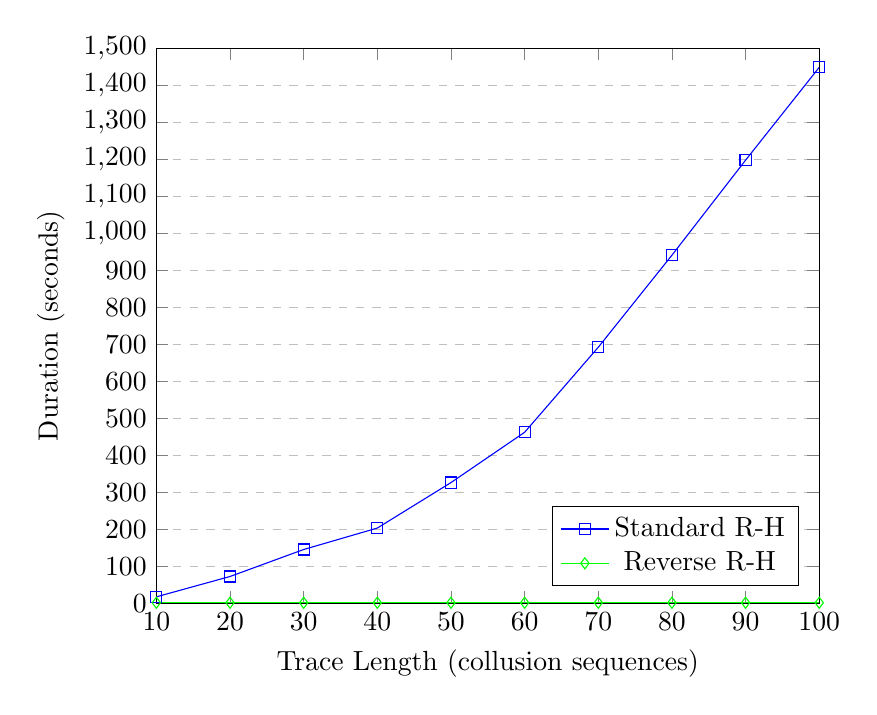
\begin{tikzpicture}
	\begin{axis}[
	    xlabel={Trace Length (collusion sequences)},
	    ylabel={Duration (seconds)},
	    xmin=10, xmax=100,
	    ymin=0, ymax=1500,
	    xtick={10,20,30,40,50,60,70,80,90,100},
	    ytick={0,100,200,300,400,500,600,700,800,900,1000,1100,1200,1300,1400,1500},
	    legend pos=south east,
	    ymajorgrids=true,
	    grid style=dashed,
	]
	
	\addplot[
	    color=blue,
	    mark=square,
	    ]
	    coordinates {
	    (10,17)(20,72)(30,145)(40,203)(50,326)(60,462)(70,692)(80,941)(90,1198)(100,1449)
	    };
	    \addlegendentry{Standard R-H}
	    
	\addplot[
	    color=green,
	    mark=diamond,
	    ]
	    coordinates {
	    (10,1)(20,1)(30,1)(40,1)(50,1)(60,1)(70,1)(80,1)(90,1)(100,1)
	    };
		\addlegendentry{Reverse R-H}
	\end{axis}
	\end{tikzpicture}
	\caption{Dependency Between Trace Length and Evaluation Duration}
	\label{fig:ReverseRHEvaluationDuration}
\end{figure}
\chapter{Implementing a Monitor Using the \RRH\ Algorithm}
\label{chap:Implementing The Monitor}

This chapter covers the implementation of a monitor that uses the \RRH\ algorithm.  We describe the classes that the monitor is composed of and illustrate the internal structure using UML diagrams.  We show evidence from practical testing that the time required to evaluate a trace in realtime remains constant regardless of trace length when using the reverse algorithm.  From this evidence we conclude that the \RRH\ enables us to construct a monitor that is capable of realtime monitoring.

\section{Monitor Design}
\label{sec:Design}

Our monitor realises the monitor process in the High Level Architecture Diagram \ref{fig:highLevelArchitectureDiagram}, on page \pageref{fig:highLevelArchitectureDiagram} and described in Section \ref{sec:Monitor} of Chapter \ref{chap:Monitoring System Architecture}.

The standard algorithm was implemented ad-hoc and without great attention to code structure.  After the lessons learned from that implementation, it became clear enough what structure the code should take for a worthwhile design to take shape.  The following UML diagrams document the classes within the monitor and the interaction between them when an event is received.

The monitor process receives events generated by the interceptor module embedded into processes by the Xposed framework.  The entry point for events in the monitor process is the EventReceiver class.

\subsection{EventReceiver Class}
\label{sec:EventReceiverClass}

The EventReceiver class is illustrated in Figure \ref{fig:eventReceiverClassDiagram}.  It is responsible for initiating the evaluation of events and reporting on the result.  The class descends from the Android BroadcastReceiver class because events are communicated to the EventReceiver by the Android intent system.  The EventReceiver class registers with the intent system for the type of intent that the interceptor broadcasts.  When the interceptor sends an intent, Android delivers the intent to the EventReceiver by calling the onReceive method with the intent as a parameter.  The EventReceiver extracts details of the event from the intent and begins evaluation.  The EventReceiver is composed of a list of Monitor classes.  In this case, the only monitor in the list is to monitor for the collusion property at the end of Section \ref{sec:ReverseCollusionFormula}.  When monitoring multiple properties, the list gets populated with a different instance of the monitor class for each property.  The EventReceiver calls the Evaluate method of every monitor, and the outcome gets returned as an EvaluationResult.  The EventReceiver reports the result to the user.

%Event Receiver Class Diagram
\begin{figure}[h]
	\centering
	
\begin{tikzpicture}[scale=0.7, every node/.style={transform shape}]
	\umlsimpleclass[alias=BroadcastReceiver]{android.content::BroadcastReceiver (abstract)}
	\umlclass[alias=EventReceiver, x=0, y=-3]{com.androidmonitor::EventReceiver}{}{+onReceive(context: Context, intent: Intent): void}
	\umlsimpleclass[alias=monitors, x=0, y=-6]{java.util::ArrayList$<$Monitor$>$}
	\umlclass[alias=Monitor, x=0, y=-9]{RosuHavelund::Monitor}
		{}
		{
			+Evaluate(traceEvent: TraceEvent): EvaluationResult\\
			+Reset(): void
		}
%	\umlsimpleclass[alias=Register, x=0, y=-13]{RosuHavelund::Register}

	\umlinherit{EventReceiver}{BroadcastReceiver}
	\umlcompo[mult1=1, arg2=-monitors, mult2=1]{EventReceiver}{monitors}
	\umluniassoc[mult2=0..n]{monitors}{Monitor}
%	\umlcompo[mult1=1, arg2=-now, mult2=1, anchor1=-130, anchor2=159]{Monitor}{Register}
%	\umlcompo[mult1=1, arg2=-previous, mult2=1, anchor1=-50, anchor2=21]{Monitor}{Register}

	\umlclass[alias=EvaluationResult, x=9, y=-1]{RosuHavelund::EvaluationResult}
		{}
		{
			+Satisfied():boolean\\
			+Message(): String\\
			+SatisfyingEvents() ArrayList$<$TraceEvent$>$
		}
	\umlsimpleclass[alias=satisfyingEvents, x=9, y=-5]{java.util::ArrayList$<$TraceEvent$>$}
	\umlclass[alias=TraceEvent, x=9, y=-9]{RosuHavelund::TraceEvent}
		{}
		{
			+Time():Date\\
			+Event(): String\\
			+Pid(): Int\\
			+AppName(): String\\
			+Action(): String\\
		}

	\umlcompo[mult1=1, arg2=-satisfyingEvents, mult2=1]{EvaluationResult}{satisfyingEvents}
	\umluniassoc[mult2=0..n]{satisfyingEvents}{TraceEvent}

	\end{tikzpicture}
	\caption{Event Receiver Class Diagram}
	\label{fig:eventReceiverClassDiagram}
\end{figure}

\subsection{Monitor Class}
\label{sec:MonitorClass}

The Monitor class is responsible for evaluating a property over a trace event.  Figure \ref{fig:monitorClassDiagram} illustrates the structure of the Monitor in detail.  The reader can observe that the Monitor class implements the \RRH\ algorithm because it is composed of the two registers, \textit{now} and \textit{previous}.  The Evaluate method performs algorithmic steps 1 and 2, described in section \ref{sec:Evaluation} earlier.  Those two steps evaluate the event over the \textit{now} register then update the \textit{previous} register.  The Monitor class returns a positive EvaluationResult if the event satisfies the formula and meets the dynamic conditions.

%Monitor Class Diagram
\begin{figure}[h]
	\centering
	\begin{tikzpicture}[scale=0.66, every node/.style={transform shape}]

		\umlclass[alias=Monitor, x=0, y=0]{RosuHavelund::Monitor}
		{}
		{
			+Monitor(formula: String, message: String, conditions: DynamicConditions)\\
			+Evaluate(traceEvent: TraceEvent): EvaluationResult\\
			+Reset(): void
		}
		
	\umlclass[alias=DynamicConditions, x=12, y=0]{RosuHavelund::DynamicConditions}
		{}
		{
			\umlvirt{\#Met(satisfyingEvents: ArrayList$<$TraceEvent$>$): ArrayList$<$TraceEvent$>$}
		}

	\umlclass[alias=CollusionConditions, x=12, y=-5]{RosuHavelund::CollusionConditions}
		{}
		{
			+Met(satisfyingEvents: ArrayList$<$TraceEvent$>$): ArrayList$<$TraceEvent$>$\\
		}

	\umlclass[alias=Register, x=0, y=-6]{RosuHavelund::Register}
		{}
		{
			+Register(expressions: ArrayList$<$Expression$>$)\\
			+Evaluate(event: String): boolean\\
			+Satisfied(): boolean\\
			+Update(register: Register): void\\
			+Reset(): void
		}

	\umlsimpleclass[alias=expressions, x=0, y=-11]{java.util::ArrayList$<$Expressions$>$}

	\umlclass[alias=Expression, x=0, y=-16]{RosuHavelund::Expression (abstract)}
		{
			+Expression(formula: String, previous: Expression)\\
			+Formula(): String\\
			+Previous(): Expression\\
			+Satisfied(): boolean\\
		}
		{
			+Evaluate(event: String): boolean\\
			+setSatisfied(satisfied: boolean)\\
			+Reset(): void\\
			+FlattenBreadthFirst(): ArrayList$<$Expression$>$
		}
		
	\umlinherit{CollusionConditions}{DynamicConditions}
	\umlcompo[mult1=1, arg2=-now, mult2=1, anchor1=-130, anchor2=121.5]{Monitor}{Register}
	\umlcompo[mult1=1, arg2=-previous, mult2=1, anchor1=-50, anchor2=58]{Monitor}{Register}
	\umlcompo[mult1=1, arg2=-dynamicConditions, pos2=0.7, mult2=1]{Monitor}{CollusionConditions}
	\umlcompo[mult1=1, arg2=-expressions, mult2=1]{Register}{expressions}
	\umluniassoc[mult2=0..n]{expressions}{Expression}

	\end{tikzpicture}
  \caption{Monitor Class Diagram}
  \label{fig:monitorClassDiagram}
\end{figure}

\subsection{Register Class}
\label{sec:RegisterClass}

Registers are arrays where each element corresponds to a subformula in breadth-first order.  The first element corresponds to the root formula, and successive elements correspond to the operands.  An important consideration is that the operands are not always immediately adjacent to the root element in the register.  The following example illustrates this consideration:\\

\begin{myEx} Distant Operands\\

The formula $\varphi = \LTLalwaysbeen((r \,S q) \rightarrow \LTLonce(q \rightarrow \LTLprevious p))$ produces subformulae:

\begin{flushleft}
$ \varphi_{1} = \LTLalwaysbeen((r \,S \,q) \rightarrow \LTLonce(q \rightarrow \LTLprevious p)) $ \\
$ \varphi_{2} = ((r \,S \,q) \rightarrow \LTLonce(q \rightarrow \LTLprevious r)) $ \\
$ \varphi_{3} = (r \,S \,q) $ \\
$ \varphi_{4} = \LTLonce(q \rightarrow \LTLprevious p) $ \\
$ \varphi_{5} = r $ \\
$ \varphi_{6} = q $ \\
$ \varphi_{7} = (q \rightarrow \LTLprevious p) $ \\
$ \varphi_{8} = q $ \\
$ \varphi_{9} = \LTLprevious p $ \\
$ \varphi_{10} = p $ 
\end{flushleft}

The register constructed from those subformulae is:

\begin{tabularx}{\textwidth}{cc|c|c|c|c|c|c|c|c|c|c|}
\centering
 & \multicolumn{1}{c}{}
 & \multicolumn{1}{c}{$ \varphi_{1}$}
 & \multicolumn{1}{c}{$ \varphi_{2}$}
 & \multicolumn{1}{c}{$ \varphi_{3}$}
 & \multicolumn{1}{c}{$ \varphi_{4}$}
 & \multicolumn{1}{c}{$ \varphi_{5}$}
 & \multicolumn{1}{c}{$ \varphi_{6}$}
 & \multicolumn{1}{c}{$ \varphi_{7}$}
 & \multicolumn{1}{c}{$ \varphi_{8}$}
 & \multicolumn{1}{c}{$ \varphi_{9}$}
 & \multicolumn{1}{c}{$ \varphi_{10}$}\\
 \cline{3-12}
 & {now} 
 & { \tikz[baseline]{\node (p1) {$\LTLalwaysbeen$};} } 
 & { \tikz[baseline]{\node (p2) {$\rightarrow$};} }  
 & { \tikz[baseline]{\node (p3) {$ S $};} }
 & { \tikz[baseline]{\node (p4) {$\LTLonce$};} }
 & { \tikz[baseline]{\node (p5) {$r$};} }
 & { \tikz[baseline]{\node (p6) {$q$};} }
 & { \tikz[baseline]{\node (p7) {$\rightarrow$};} }
 & { \tikz[baseline]{\node (p8) {$q$};} }
 & { \tikz[baseline]{\node (p9) {$\LTLprevious$};} }
 & { \tikz[baseline]{\node (p10) {$p$};} } \\
 \cline{3-12}
\end{tabularx}
\begin{tikzpicture}[overlay]
    \draw[red, thick,->] (p1) edge[bend left=10] (p2);
    \draw[red, thick,->] (p2) edge[bend left=10] (p3);
    \draw[red, thick,->] (p2) edge[bend right=30] (p4);
    \draw[red, thick,->] (p3) edge[bend left=30]  (p5);
    \draw[red, thick,->] (p3) edge[bend right=30] (p6);
    \draw[red, thick,->] (p4)[bend left=20] edge (p7);
    \draw[red, thick,->] (p7)[bend left=10] edge (p8);
    \draw[red, thick,->] (p7)[bend right=30] edge (p9);
    \draw[red, thick,->] (p9)[bend left=10] edge (p10);
\end{tikzpicture}
\\\\
The arrows indicate which elements in the register are the operands of another element.  We can see the first element, $\varphi_1$, has the unary has-always-been operator at its root.  In that case, its operand is indeed the adjacent element $\varphi_2$.  But $\varphi_2$ is a binary implies formula with two subformulae as operands.  The satisfaction of $\varphi_2$ is dependent on the immediately adjacent $\varphi_3$ and also on the distant element $\varphi_4$.  And the satisfaction of $\varphi_4$ depends on the satisfaction of distant $\varphi_7$.

\qed
\end{myEx}

To reference the subformulae of a formula is not a trivial exercise of simply referencing the adjacent element in the register.  Instead, the element corresponding to that subformula may be any of the following elements.  When evaluating each element within the register, the challenge is finding the elements corresponding to the operands.  The solution is to make each element of the register a composition that we call an expression.

\subsection{Expression Classes}
\label{sec:ExpressionClasses}

Expressions are responsible for determining the satisfaction of a formula by an event.  They implement operator semantics and present the operands of a formula as references to other expressions.  Every LTL operator we implement has a subclass of expression somewhere within the hierarchical structure shown in class diagram \ref{fig:expressionHierarchy}.

% Expression Hierarchy Class Diagram
\begin{figure}[h!]
	\centering
	
\begin{tikzpicture}[scale=0.55, every node/.style={transform shape}]
	
		\umlclass[alias=Expression, x=-8, y=0]{RosuHavelund::Expression (abstract)}
		{
			+Formula(): String\\
			+Previous(): Expression\\
			+Satisfied(): boolean\\
		}
		{
			+Evaluate(event: String): boolean\\
			+setSatisfied(satisfied: boolean)\\
			+Reset(): void\\
			+FlattenBreadthFirst(): ArrayList$<$Expression$>$
		}

		\umlclass[alias=UnaryExpression, x=-2, y=-5]{RosuHavelund::UnaryExpression (abstract)}
		{
			+Operator(): String\\
			+LeftOperand(): Expression\\
		}
		{}
		\umlinherit[geometry=-|]{UnaryExpression}{Expression}

		\umlclass[alias=LiteralExpression, x=-13, y=-5]{RosuHavelund::LiteralExpression}
		{}
		{
			\umlstatic{+Match(formula: String): boolean}\\
			\umlstatic{+MatchPosition(formula: String): int}\\
		}
		\umlinherit[geometry=-|]{LiteralExpression}{Expression}

		\umlclass[alias=BinaryExpression, x=2, y=-9]{RosuHavelund::BinaryExpression (abstract)}
		{
			+RightOperand(): Expression\\
		}
		{}
		\umlinherit[geometry=-|, anchors=180 and -140]{BinaryExpression}{UnaryExpression}

		\umlclass[alias=NotExpression, x=-9, y=-9]{RosuHavelund::NotExpression}
		{}
		{
			\umlstatic{+Match(formula: String): boolean}\\
			\umlstatic{+MatchPosition(formula: String): int}\\
		}
		\umlinherit[geometry=-|, anchors=0 and -140]{NotExpression}{UnaryExpression}

		\umlclass[alias=AlwaysBeenExpression, x=-9, y=-13]{RosuHavelund::AlwaysBeenExpression}
		{}
		{
			\umlstatic{+Match(formula: String): boolean}\\
			\umlstatic{+MatchPosition(formula: String): int}\\
		}
		\umlinherit[geometry=-|, anchors=0 and -140]{AlwaysBeenExpression}{UnaryExpression}

		\umlclass[alias=OnceExpression, x=-9, y=-17]{RosuHavelund::OnceExpression}
		{}
		{
			\umlstatic{+Match(formula: String): boolean}\\
			\umlstatic{+MatchPosition(formula: String): int}\\
		}
		\umlinherit[geometry=-|, anchors=0 and -140]{OnceExpression}{UnaryExpression}

		\umlclass[alias=PreviousExpression, x=-9, y=-21]{RosuHavelund::PreviousExpression}
		{}
		{
			\umlstatic{+Match(formula: String): boolean}\\
			\umlstatic{+MatchPosition(formula: String): int}\\
		}
		\umlinherit[geometry=-|, anchors=0 and -140]{PreviousExpression}{UnaryExpression}
	
		\umlclass[alias=AndExpression, x=6, y=-13]{RosuHavelund::AndExpression}
		{}
		{
			\umlstatic{+Match(formula: String): boolean}\\
			\umlstatic{+MatchPosition(formula: String): int}\\
		}
		\umlinherit[geometry=-|, anchors=180 and -140]{AndExpression}{BinaryExpression}

		\umlclass[alias=OrExpression, x=6, y=-17]{RosuHavelund::OrExpression}
		{}
		{
			\umlstatic{+Match(formula: String): boolean}\\
			\umlstatic{+MatchPosition(formula: String): int}\\
		}
		\umlinherit[geometry=-|, anchors=180 and -140]{OrExpression}{BinaryExpression}

		\umlclass[alias=ImpliesExpression, x=6, y=-21]{RosuHavelund::ImpliesExpression}
		{}
		{
			\umlstatic{+Match(formula: String): boolean}\\
			\umlstatic{+MatchPosition(formula: String): int}\\
		}
		\umlinherit[geometry=-|, anchors=180 and -140]{ImpliesExpression}{BinaryExpression}
		
		\umlclass[alias=SinceExpression, x=6, y=-25]{RosuHavelund::SinceExpression}
		{}
		{
			\umlstatic{+Match(formula: String): boolean}\\
			\umlstatic{+MatchPosition(formula: String): int}\\
		}
		\umlinherit[geometry=-|, anchors=180 and -140]{SinceExpression}{BinaryExpression}
	\end{tikzpicture}
 	\caption{Expression Hierarchy}
 	\label{fig:expressionHierarchy}
\end{figure}

At the top level of the class hierarchy, there is an abstract expression class composed of a formula string, a boolean to indicate if an event satisfies that formula, and a reference to the same expression in the \textit{previous} register.  Temporal operators make use of the Previous expression during evaluation.  Literal expressions and unary expressions are extensions of the abstract expression class.  Literals have no operator or operands, and unary expressions have an operator and a left operand.  Binary expressions are a derivative of unary expressions and add the right operand.  The operands of an expression are references to other expressions within the register and Section \ref{sec:MonitorConstruction} will describe how they get made.  

All expressions have an Evaluate method responsible for returning whether the event parameter satisfies that expressions formula, according to the semantics of the outermost operator.

\subsection{Monitor Construction}
\label{sec:MonitorConstruction}

When the monitor process gets launched, the process entry point constructs a monitor for the collusion formula defined in Section \ref{sec:ReverseCollusionFormula}.  The collusion formula and an instance of the dynamic conditions related to that formula get passed to the monitor's constructor.  Instantiation of the monitor class begins a cascade of object instantiations that result in the structure shown in Figure \ref{fig:monitorClassDiagram}.

The monitor class uses a class factory to construct two syntax trees from the formula.  The class factory contains all the concrete subclasses of the expression class shown in Figure \ref{fig:expressionHierarchy}.  It returns an instance of the expression whose operator is at the root of the formula.  The class factory does this by iterating through the registered expression classes, calling the static match method on each, until it finds the expression whose operator matches the outermost\footnote{The outermost operator gets identified as the operator outside all braces} operator of the formula.  The match method is static because we do not wish to construct an instance of the class only to discover the operator does not match the operator of the formula.  When the matching expression gets found, the class factory constructs an instance and passes the formula string to the constructor.  The expression constructor recognises the formula operands as the substrings to the left and right of the outermost operator.  It constructs child expressions for the operands by calling the class factory again with each substring.  Syntax tree construction recurses until it reaches leaf nodes with no operator or operands.  The class factory then constructs a literal class with no child nodes, and the syntax tree is complete.

Monitor constructor then continues by creating the \textit{now} and \textit{previous} registers from the tree structures.  Each tree gets flattened into a breadth-first ordered array of expressions by calling the flatten method on the root node of each tree.  The flatten method traverses the tree in breadth-first order and puts each node into an array.  As mentioned earlier, the operands of each expression are references to child expressions in the tree.  After the tree gets flattened into an array, the references point to other array elements.  It is then easy to reach operands elsewhere in the register.

The semantics of the temporal operators, such as has-always-been and once, involve earlier evaluations.  The \textit{previous} register keeps track of earlier evaluations therefore the \textit{now} register needs a reference to it.  The syntax tree for the \textit{previous} register gets constructed first, and the root expression gets passed to the constructor of the \textit{now} tree that is constructed second.  As each node in the \textit{now} tree is constructed, the \textit{previous} tree is traversed in unison.  A reference to the corresponding node from the \textit{previous} tree is passed to the constructor of each \textit{now} tree node and held.  The reference is called Previous and can be seen in the expression class in Figures \ref{fig:monitorClassDiagram} and \ref{fig:expressionHierarchy}.  When the trees get flattened into registers, the expressions from the \textit{previous} register are available to the corresponding expressions in the \textit{now} register during evaluation.

\subsection{Performing an Evaluation}
\label{sec:PerformingAnEvaluation}

The sequence diagram in Figure \ref{fig:monitorSequenceDiagram} illustrates the evaluation of an event in detail.  The EventReceiver class in the monitor process receives an event from the interceptor.  The EventReceiver passes the event to the monitor by calling its Evaluate method.  In turn, the monitor delegates evaluation to its \textit{now} register by calling its Evaluate method.  The \textit{now} register iterates through each expression, from the last to the first, calling the expression's Evaluate method and passing the event.  The result of the expression's Evaluate method gets determined by the semantics of the expression's operator from Definition \ref{def:PastNon-emptyTraceSemantics}.  The result gets assigned to the expression's Satisfied member and returned to the register.

After the event has been evaluated by all expressions within the \textit{now} register, execution returns to the monitor.  The result of evaluating over the \textit{now} register gets accumulated into the \textit{previous} register by calling the Update method on the \textit{previous} register and passing the \textit{now} register.  The Update method iterates through all the expressions within the \textit{previous} register and assigns a value to the Satisfied member from the corresponding member in the \textit{next} register.

After updating the \textit{previous} register, the Evaluate method of the monitor is complete, and it returns an EvaluationResult to the EventReceiver.  The EvaluationResult comprises a boolean to indicate satisfaction of the formula and the list of events that contributed to satisfaction.

If the EvaluationResult confirms the formula is satisfied, the user gets notified that possible collusion is detected.  The monitor then gets reset so that it can recognise more collusion attacks.  It gets reset by assigning values to the Satisfied members of expressions in the \textit{now} and \textit{previous} registers that are arrived at when evaluating an empty trace.  The effect is that the monitor will continue as if it has never seen any events.  It will recognise future attacks but not recognise attacks in progress when the monitor got satisfied.  An alternative method to reset the monitor is to remove the events that satisfied the monitor from the trace, and reevaluate the remaining trace.  The monitor would then recognise other collusion attacks in progress when the monitor was satisfied as well as future attacks.

% Event evaluation sequence diagram
\begin{figure}[h]
	\begin{resizedtikzpicture}{\textwidth}
		\begin{umlseqdiag}
		\umlactor[class=Process]{app}
		\umlobject[class=Interceptor]{interceptor}
		\umlactor[class=Process]{monitorProcess}
		\umlobject[class=EventReceiver]{receiver}
		\umlmulti[class=Monitor]{monitor}
		\umlmulti[class=Register]{register}
		\umlmulti[class=Expression]{expression}
		\umlobject[class=CollusionConditions, x=30]{dynamicConditions}
		\begin{umlcall}[op={action}]{app}{interceptor}
			\begin{umlcall}[op={intent}]{interceptor}{monitorProcess}
				\begin{umlcall}[op={onReceive(intent)}]{monitorProcess}{receiver}
		
					\begin{umlfragment}[type=loop, label=foreach monitor]
					
						\begin{umlcall}[op={Evaluate(event)}, return=result]{receiver}{monitor}
							\begin{umlcall}[op={now.Evaluate(event)}, return=result]{monitor}{register}
								\begin{umlfragment}[type=loop, label=foreach expression, inner xsep=7]
									\begin{umlcall}[op={Evaluate(event)}, return=result]{register}{expression}\end{umlcall}
								\end{umlfragment}
							\end{umlcall}
							\begin{umlcall}[op={previous.Update()}]{monitor}{register}\end{umlcall}
							
							\begin{umlfragment}[type=opt, label=if previous.Satisfied, inner xsep=7]
								\begin{umlcall}[op={Met(satisfyingEvents)}, return=satisfyingEvents]{monitor}{dynamicConditions}\end{umlcall}			
							\end{umlfragment}
						\end{umlcall}
					
						\begin{umlfragment}[type=opt, label=if result.Satisfied, inner xsep=4]
							\begin{umlcall}[op={Reset()}]{receiver}{monitor}
								\begin{umlcall}[op={now.Reset()}]{monitor}{register}
									\begin{umlfragment}[type=loop, label=foreach expression, inner xsep=7]
										\begin{umlcall}[op={Reset()}]{register}{expression}\end{umlcall}
									\end{umlfragment}
								\end{umlcall}
								
								\begin{umlcall}[op={previous.Reset()}]{monitor}{register}
									\begin{umlfragment}[type=loop, label=foreach expression, inner xsep=7]
										\begin{umlcall}[op={Reset()}]{register}{expression}\end{umlcall}
									\end{umlfragment}
								\end{umlcall}
							\end{umlcall}
						\end{umlfragment}
						
					\end{umlfragment}
			\end{umlcall}
			\end{umlcall}
		\end{umlcall}
		\end{umlseqdiag}
	\end{resizedtikzpicture}
    \caption{Evaluation of an Action}
    \label{fig:monitorSequenceDiagram}
\end{figure}

\section{Testing the \RRH\ Algorithm}
\label{sec:Testing The Reverse Rosu-Havelund Algorithm}

We performed similar functional tests on the reverse algorithm to those for the standard \RH\ algorithm, except that tests for future operators got replaced with tests for past operators.

Test cases got generated manually by applying the semantics of each operator, from section \ref{sec:LTLPastSemantics} to a series of traces and noting the expected result.  The test cases are in appendix \ref{app:RRHFunctionalTestCases}.  For practical use, it was necessary to replace some of the LTL symbols with characters available on the keyboard.  Table \ref{tab:AlternativeLTLOperators} provides the translation.

The tests were run by entering the formula and test traces from each test case into a test harness application.  The test harness then evaluated the formula over each trace using the \RRH\ implementation and wrote the results to the console window.  The results are in appendix \ref{app:RRHFunctionalTestResults} and the test harness code is in \ref{app:RRHCode}.  The results confirm the functionality is identical to that of the standard algorithm with respect to the classical logical operators and the functioning of the past temporal operators is as expected.

We also ran the same performance tests as those in section \ref{subsec:PracticalPerformanceAnalysisExecution} on the \RRH\ algorithm.  We used the reader and publisher apps to generate traces of increasing length and measured the time taken to evaluate each trace.

\subsection{Test Results}
\label{subsec:PracticalPerformanceAnalysisResultsRRH}

Table \ref{tab:ReverseRHExecutionTimes} gives the performance test results.  The time taken to evaluate each trace remained constant at less than a second, regardless of the size of the trace.

\begin{table}[h!]
	\centering
	\captionsetup{width=0.6\linewidth, justification=centering}
	\begin{tabular}{r|r} 
	Trace Length  & Duration\\
	(collusion sequences) & (seconds)\\
	\hline
	10 & $<1$\\
	20 & $<1$\\
	30 & $<1$\\
	40 & $<1$\\
	50 & $<1$\\
	60 & $<1$\\
	70 & $<1$\\
	80 & $<1$\\
	90 & $<1$\\
	100 & $<1$\\
	\hline
	\end{tabular}
	\caption{Duration of the \RRH\ Algorithm Evaluating Traces of Increasing Length}
	\label{tab:ReverseRHExecutionTimes}
\end{table}

%\newpage

\section{Scalability of the \RRH\ Algorithm}
\label{sec:Scalability Of Reverse Rosu-Havelund Algorithm}

Figure \ref{fig:ReverseRHEvaluationDuration} compares the performance of the standard \RH\ algorithm, plotted by the blue curve, with that of the \RRH\ algorithm, plotted by the flat green curve.  The results are in line with our expectations of the reverse algorithm and support its suitability for realtime monitoring.

\begin{figure}[h!]
	\centering
	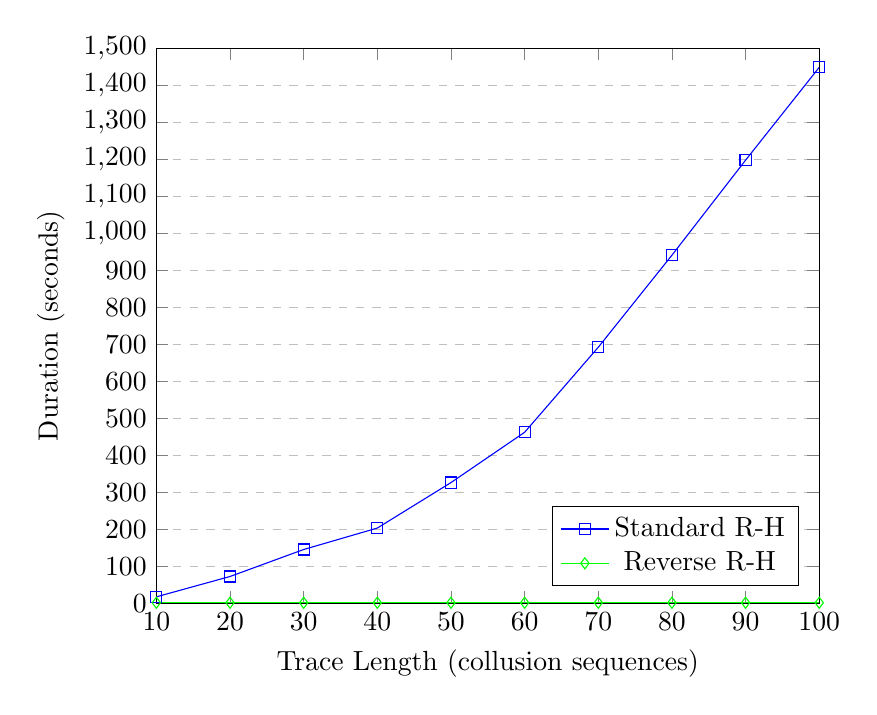
\begin{tikzpicture}
	\begin{axis}[
	    xlabel={Trace Length (collusion sequences)},
	    ylabel={Duration (seconds)},
	    xmin=10, xmax=100,
	    ymin=0, ymax=1500,
	    xtick={10,20,30,40,50,60,70,80,90,100},
	    ytick={0,100,200,300,400,500,600,700,800,900,1000,1100,1200,1300,1400,1500},
	    legend pos=south east,
	    ymajorgrids=true,
	    grid style=dashed,
	]
	
	\addplot[
	    color=blue,
	    mark=square,
	    ]
	    coordinates {
	    (10,17)(20,72)(30,145)(40,203)(50,326)(60,462)(70,692)(80,941)(90,1198)(100,1449)
	    };
	    \addlegendentry{Standard R-H}
	    
	\addplot[
	    color=green,
	    mark=diamond,
	    ]
	    coordinates {
	    (10,1)(20,1)(30,1)(40,1)(50,1)(60,1)(70,1)(80,1)(90,1)(100,1)
	    };
		\addlegendentry{Reverse R-H}
	\end{axis}
	\end{tikzpicture}
	\caption{Dependency Between Trace Length and Evaluation Duration}
	\label{fig:ReverseRHEvaluationDuration}
\end{figure}
\chapter{Demonstrating the Monitor in Action}
\label{chap:MonitorInAction}

In this chapter we present the culmination of our efforts with a demonstration of the monitor detecting a collusion attack.

\section{Installation}

\begin{wrapfigure}[15]{r}{0.44\linewidth}
	\centering
	\vspace{-12pt}
	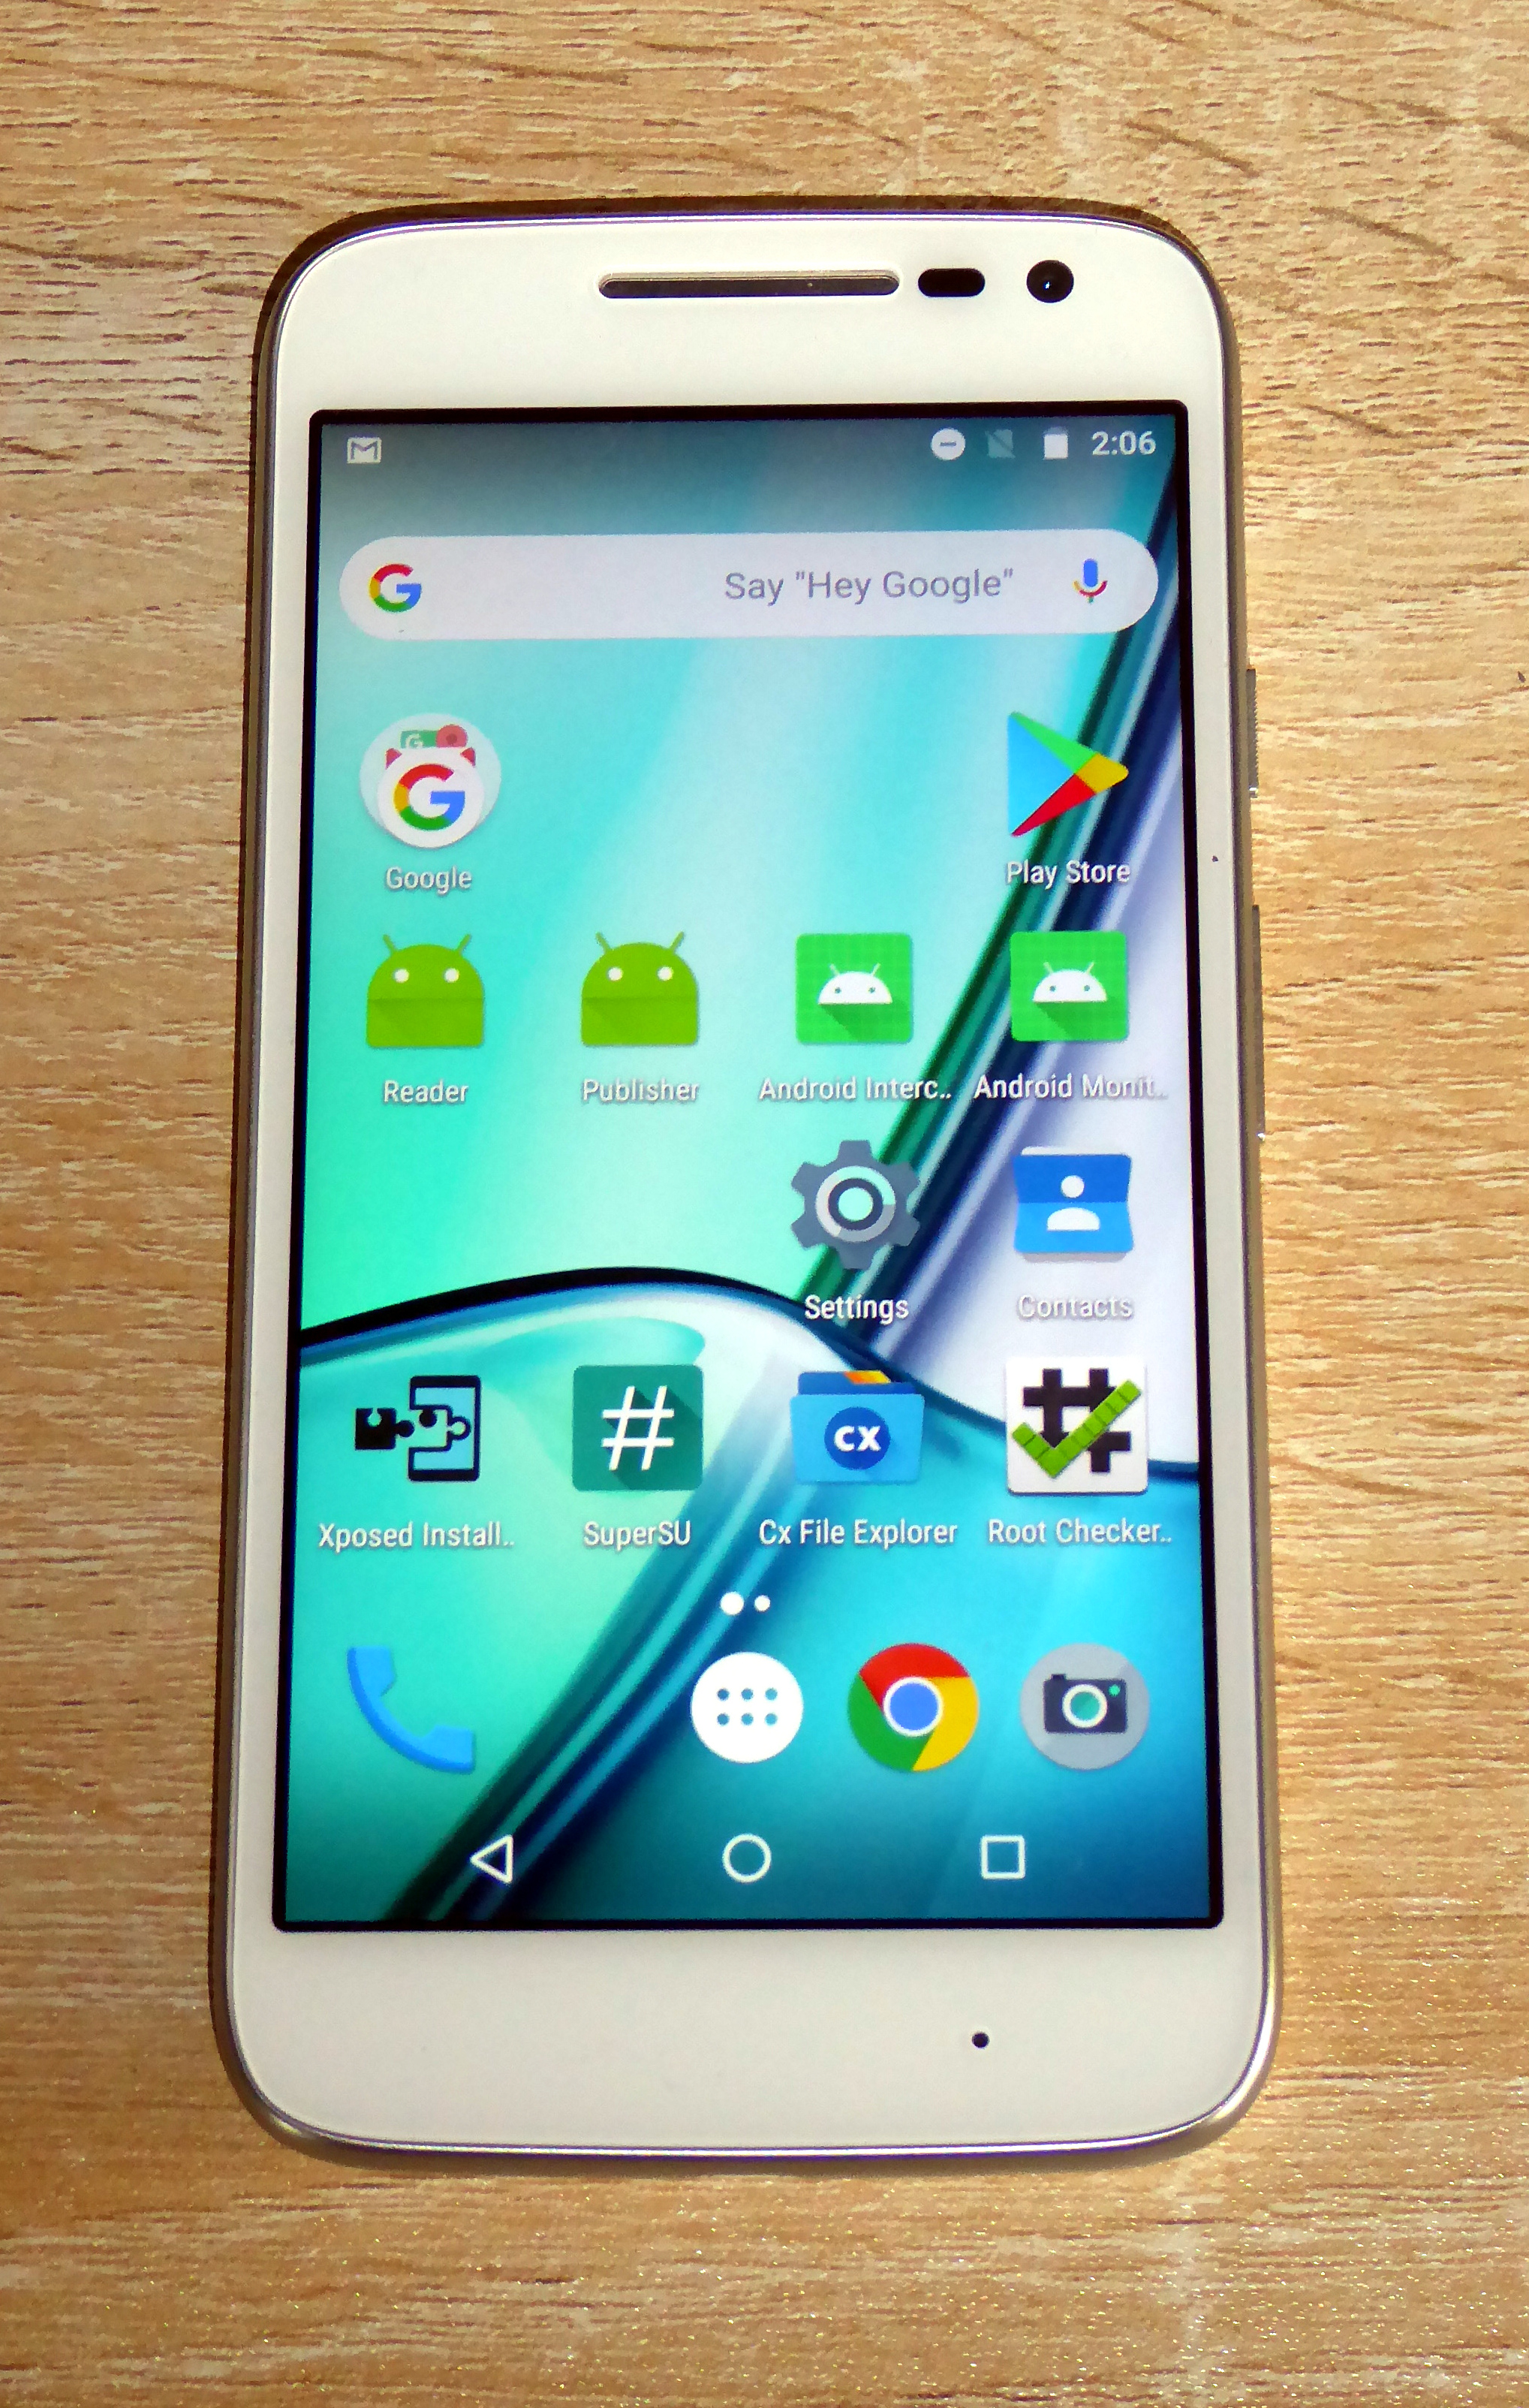
\includegraphics[height=0.39\textheight]{graphics/PhonePhotos/01 - Installation.jpg}
	\caption{Monitor Installed}
	\label{fig:MonitorInstalled}
\end{wrapfigure}

To demonstrate the monitor in action it is necessary to stage collusion attacks at will.  We used the reader and publisher applications that we developed earlier to perform the attack.  They were both installed onto a rooted Motorola G4 Play phone running Android 6.0.1, along with the interceptor module and the monitor.  Figure \ref{fig:MonitorInstalled} shows the installation.  We also added two contacts to the phone's contact list, shown in Figure \ref{fig:DisplayingContacts}.

\section{Before Collusion}

Figure \ref{fig:BeforeCollusion} shows the state of the phone before the attack.  The publisher in Figure \ref{fig:PublisherBefore} is ready to receive contacts.  The monitor is active in Figure \ref{fig:MonitorBefore} but has not yet detected collusion.\\

\begin{figure}[h!]
	\centering
	\begin{subfigure}{0.49\textwidth}
	  \centering
      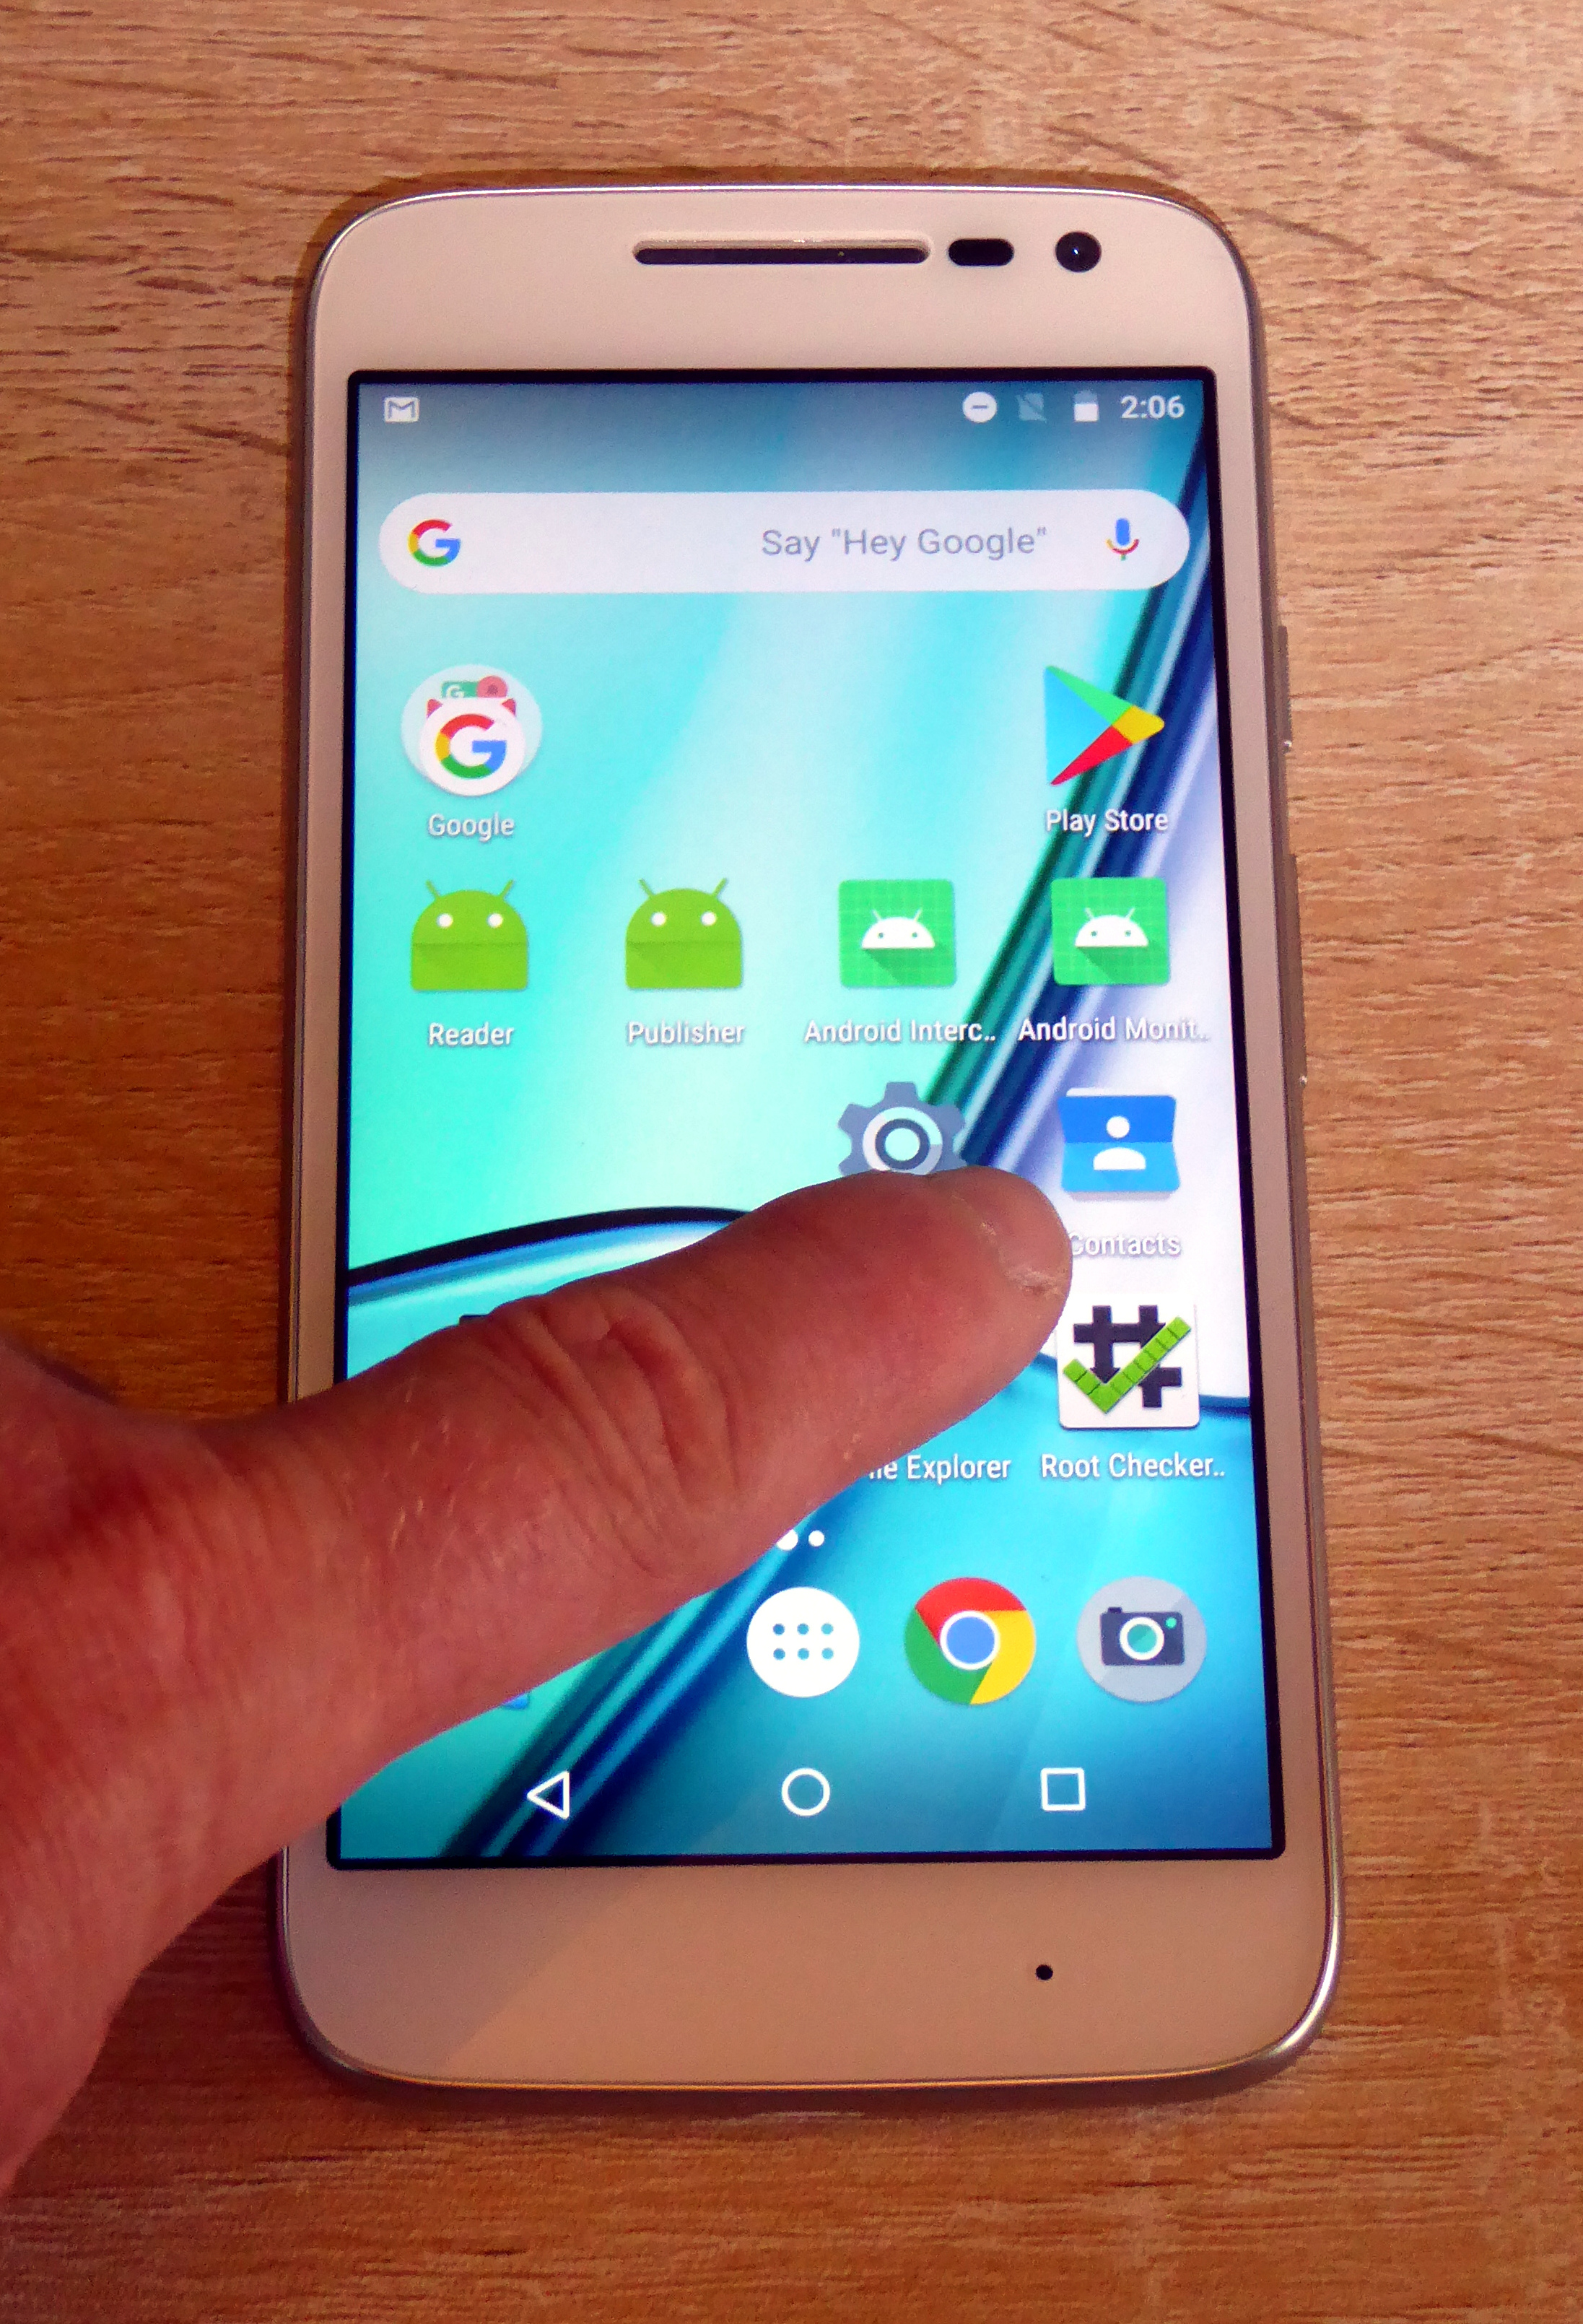
\includegraphics[height=0.45\textheight]{graphics/PhonePhotos/02 - BringUpContacts.jpg}
      \caption{Opening the Contacts List}
      \label{fig:OpeningContacts}
	\end{subfigure}
\hfill	
	\begin{subfigure}{0.49\textwidth}
		\centering
        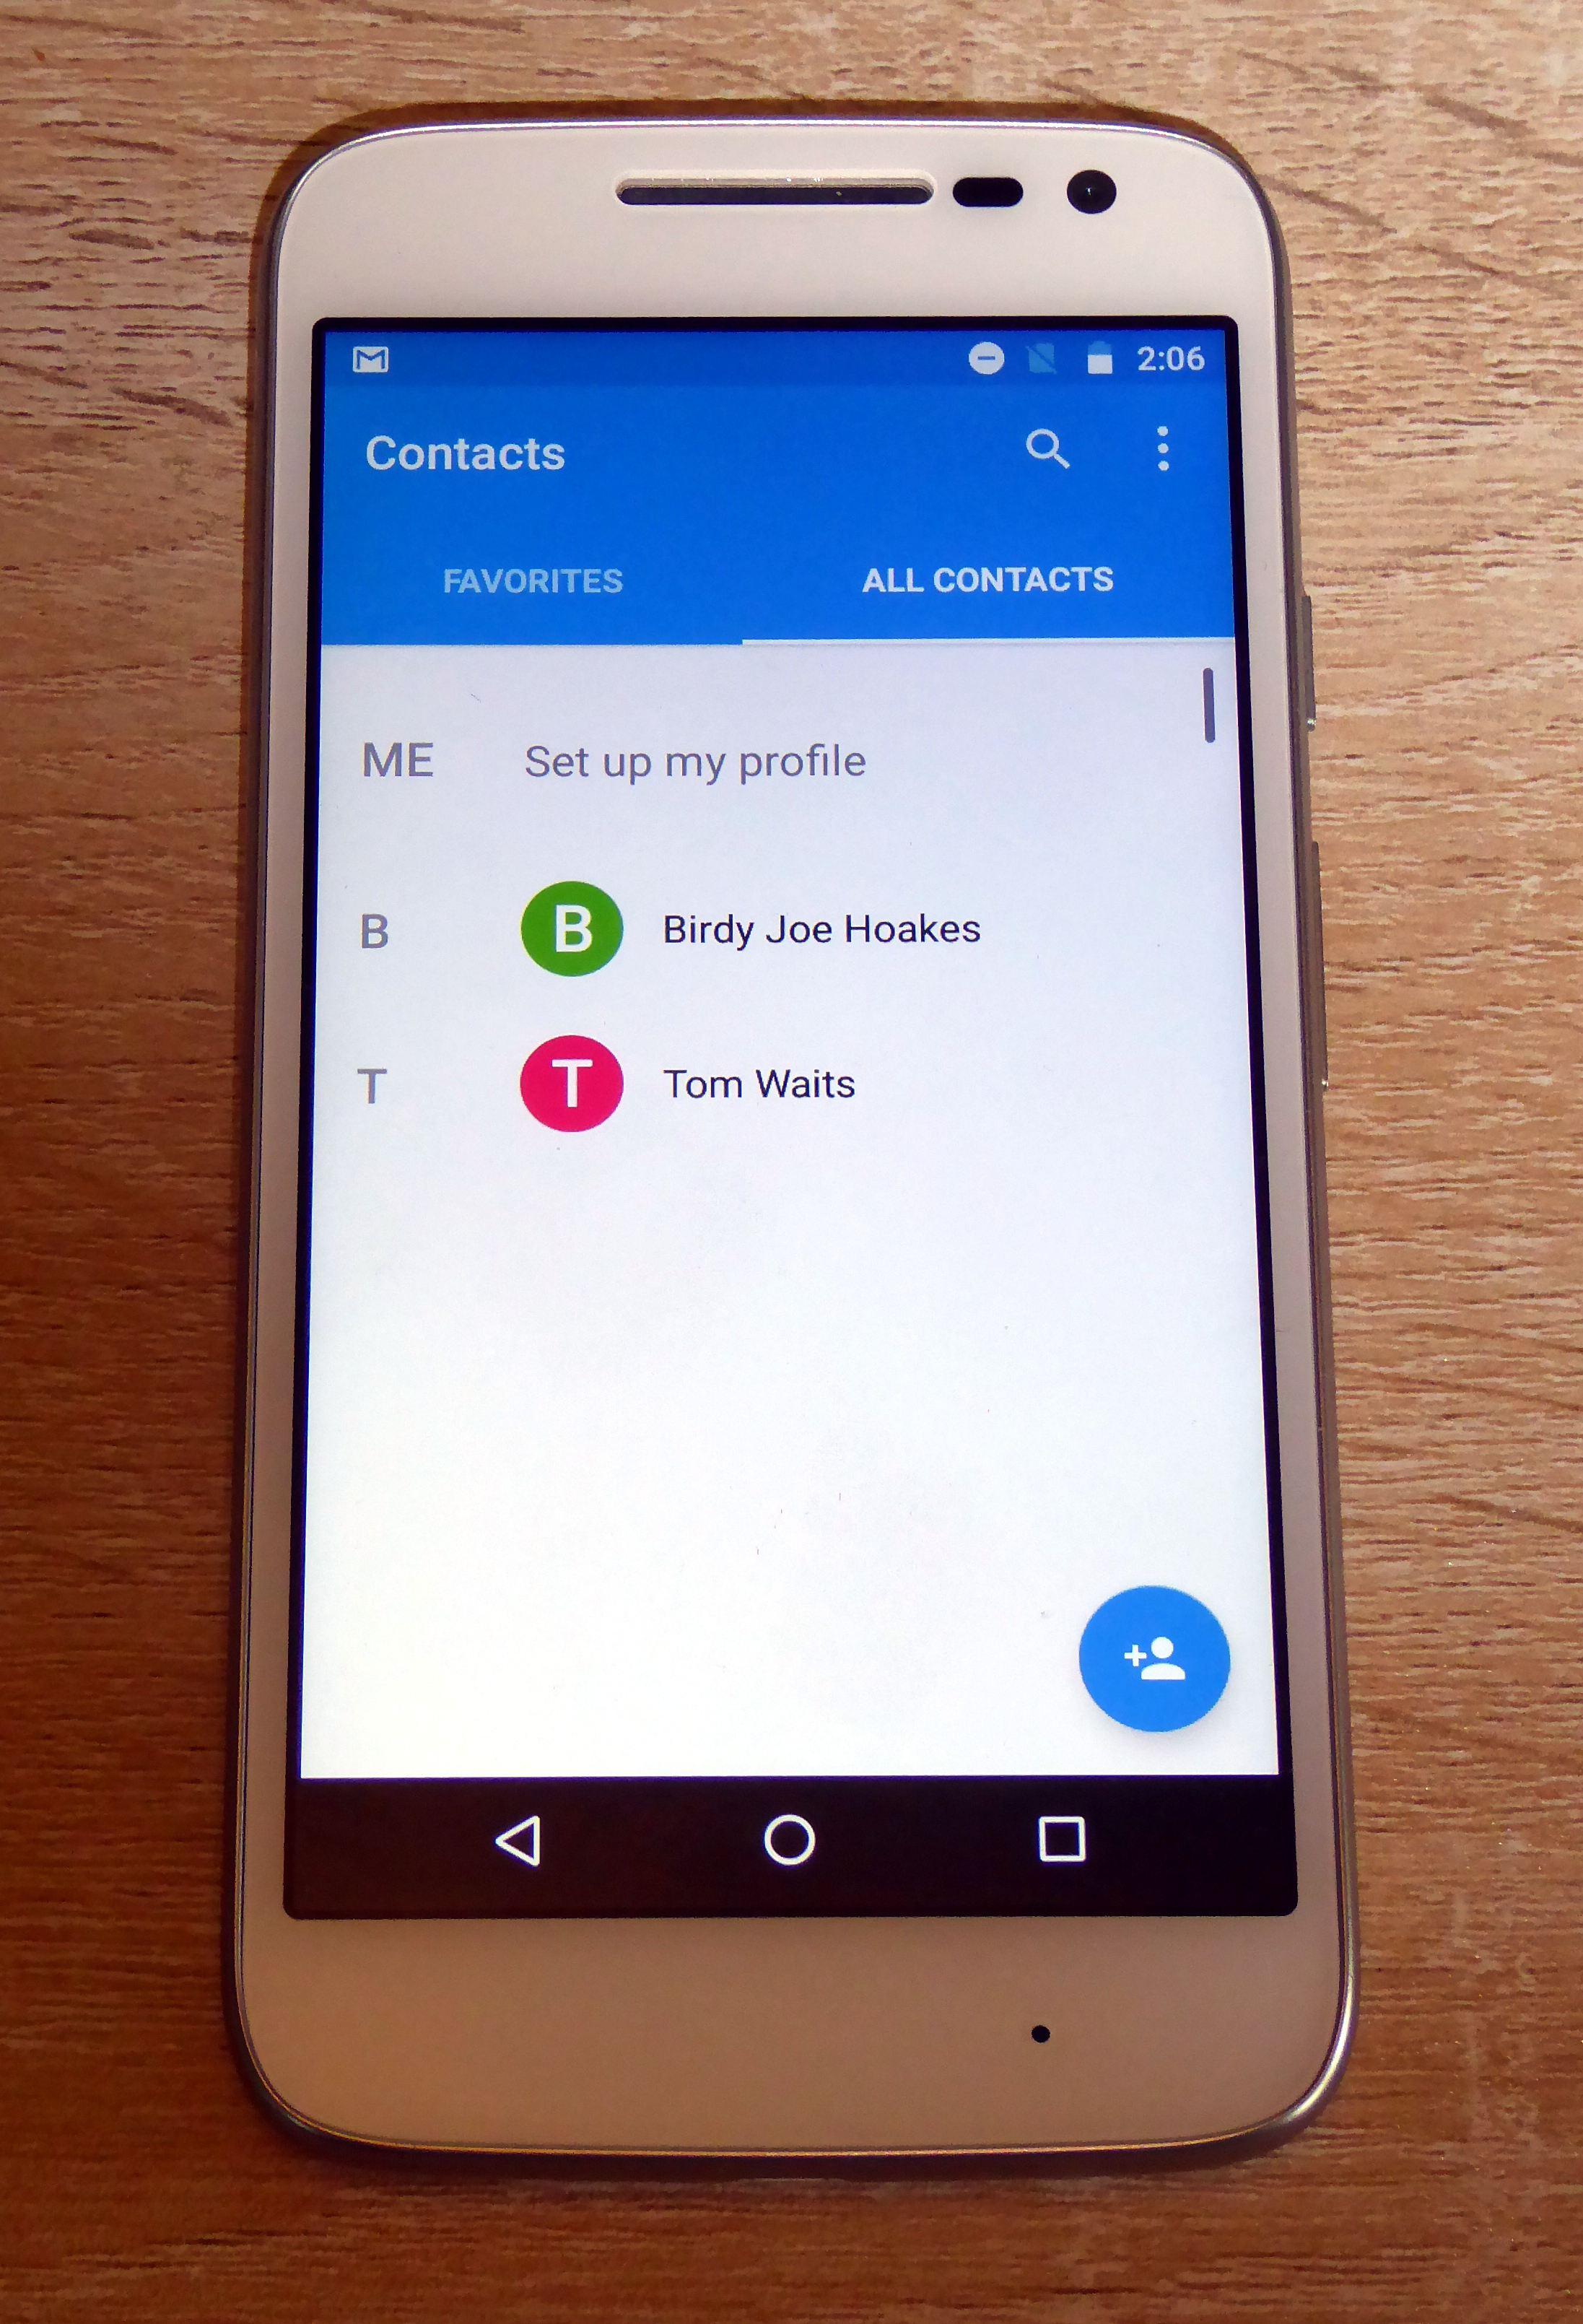
\includegraphics[height=0.45\textheight]{graphics/PhonePhotos/03 - DisplayContacts.jpg}
        \caption{Displaying the Contacts}
        \label{fig:DisplayingContacts}
	\end{subfigure}
	\caption{Stored Contacts List}
	\label{fig:ContactsList}
\end{figure}

We started the collusion attack manually by telling the reader app to send the contacts.  Figure \ref{fig:ReaderSend} shows us sending the contacts list by pressing the send button on the reader.  The publisher app completed the attack when it received the contacts and displayed them on the screen.  We can see in Figure \ref{fig:PublisherAfter} that this happened because the publisher log confirms it received two contacts, identical to those displayed on the reader app.  And we can see it has put them on the screen.

\section{After Collusion}

While the attack was in progress, the interceptor module intercepted the operating system calls used to perform the attack and informed the monitor by sending it trace events.  The monitor writes a log entry for every event it receives and entries for the trace evaluation result.  Figure \ref{fig:MonitorAfter} shows the monitor application and the log it generated during the attack.  

The log entry highlighted by the red rectangle is an alert that indicates the monitor has successfully detected a complete attack sequence.  The log entries immediately before the alert show the complete attack sequence (q,s,r,p) and the log entries immediately after the alert list the trace events that caused the monitor to be triggered.

\newpage

\begin{figure}[H]
	\centering
	\begin{subfigure}{0.49\textwidth}
		\centering
		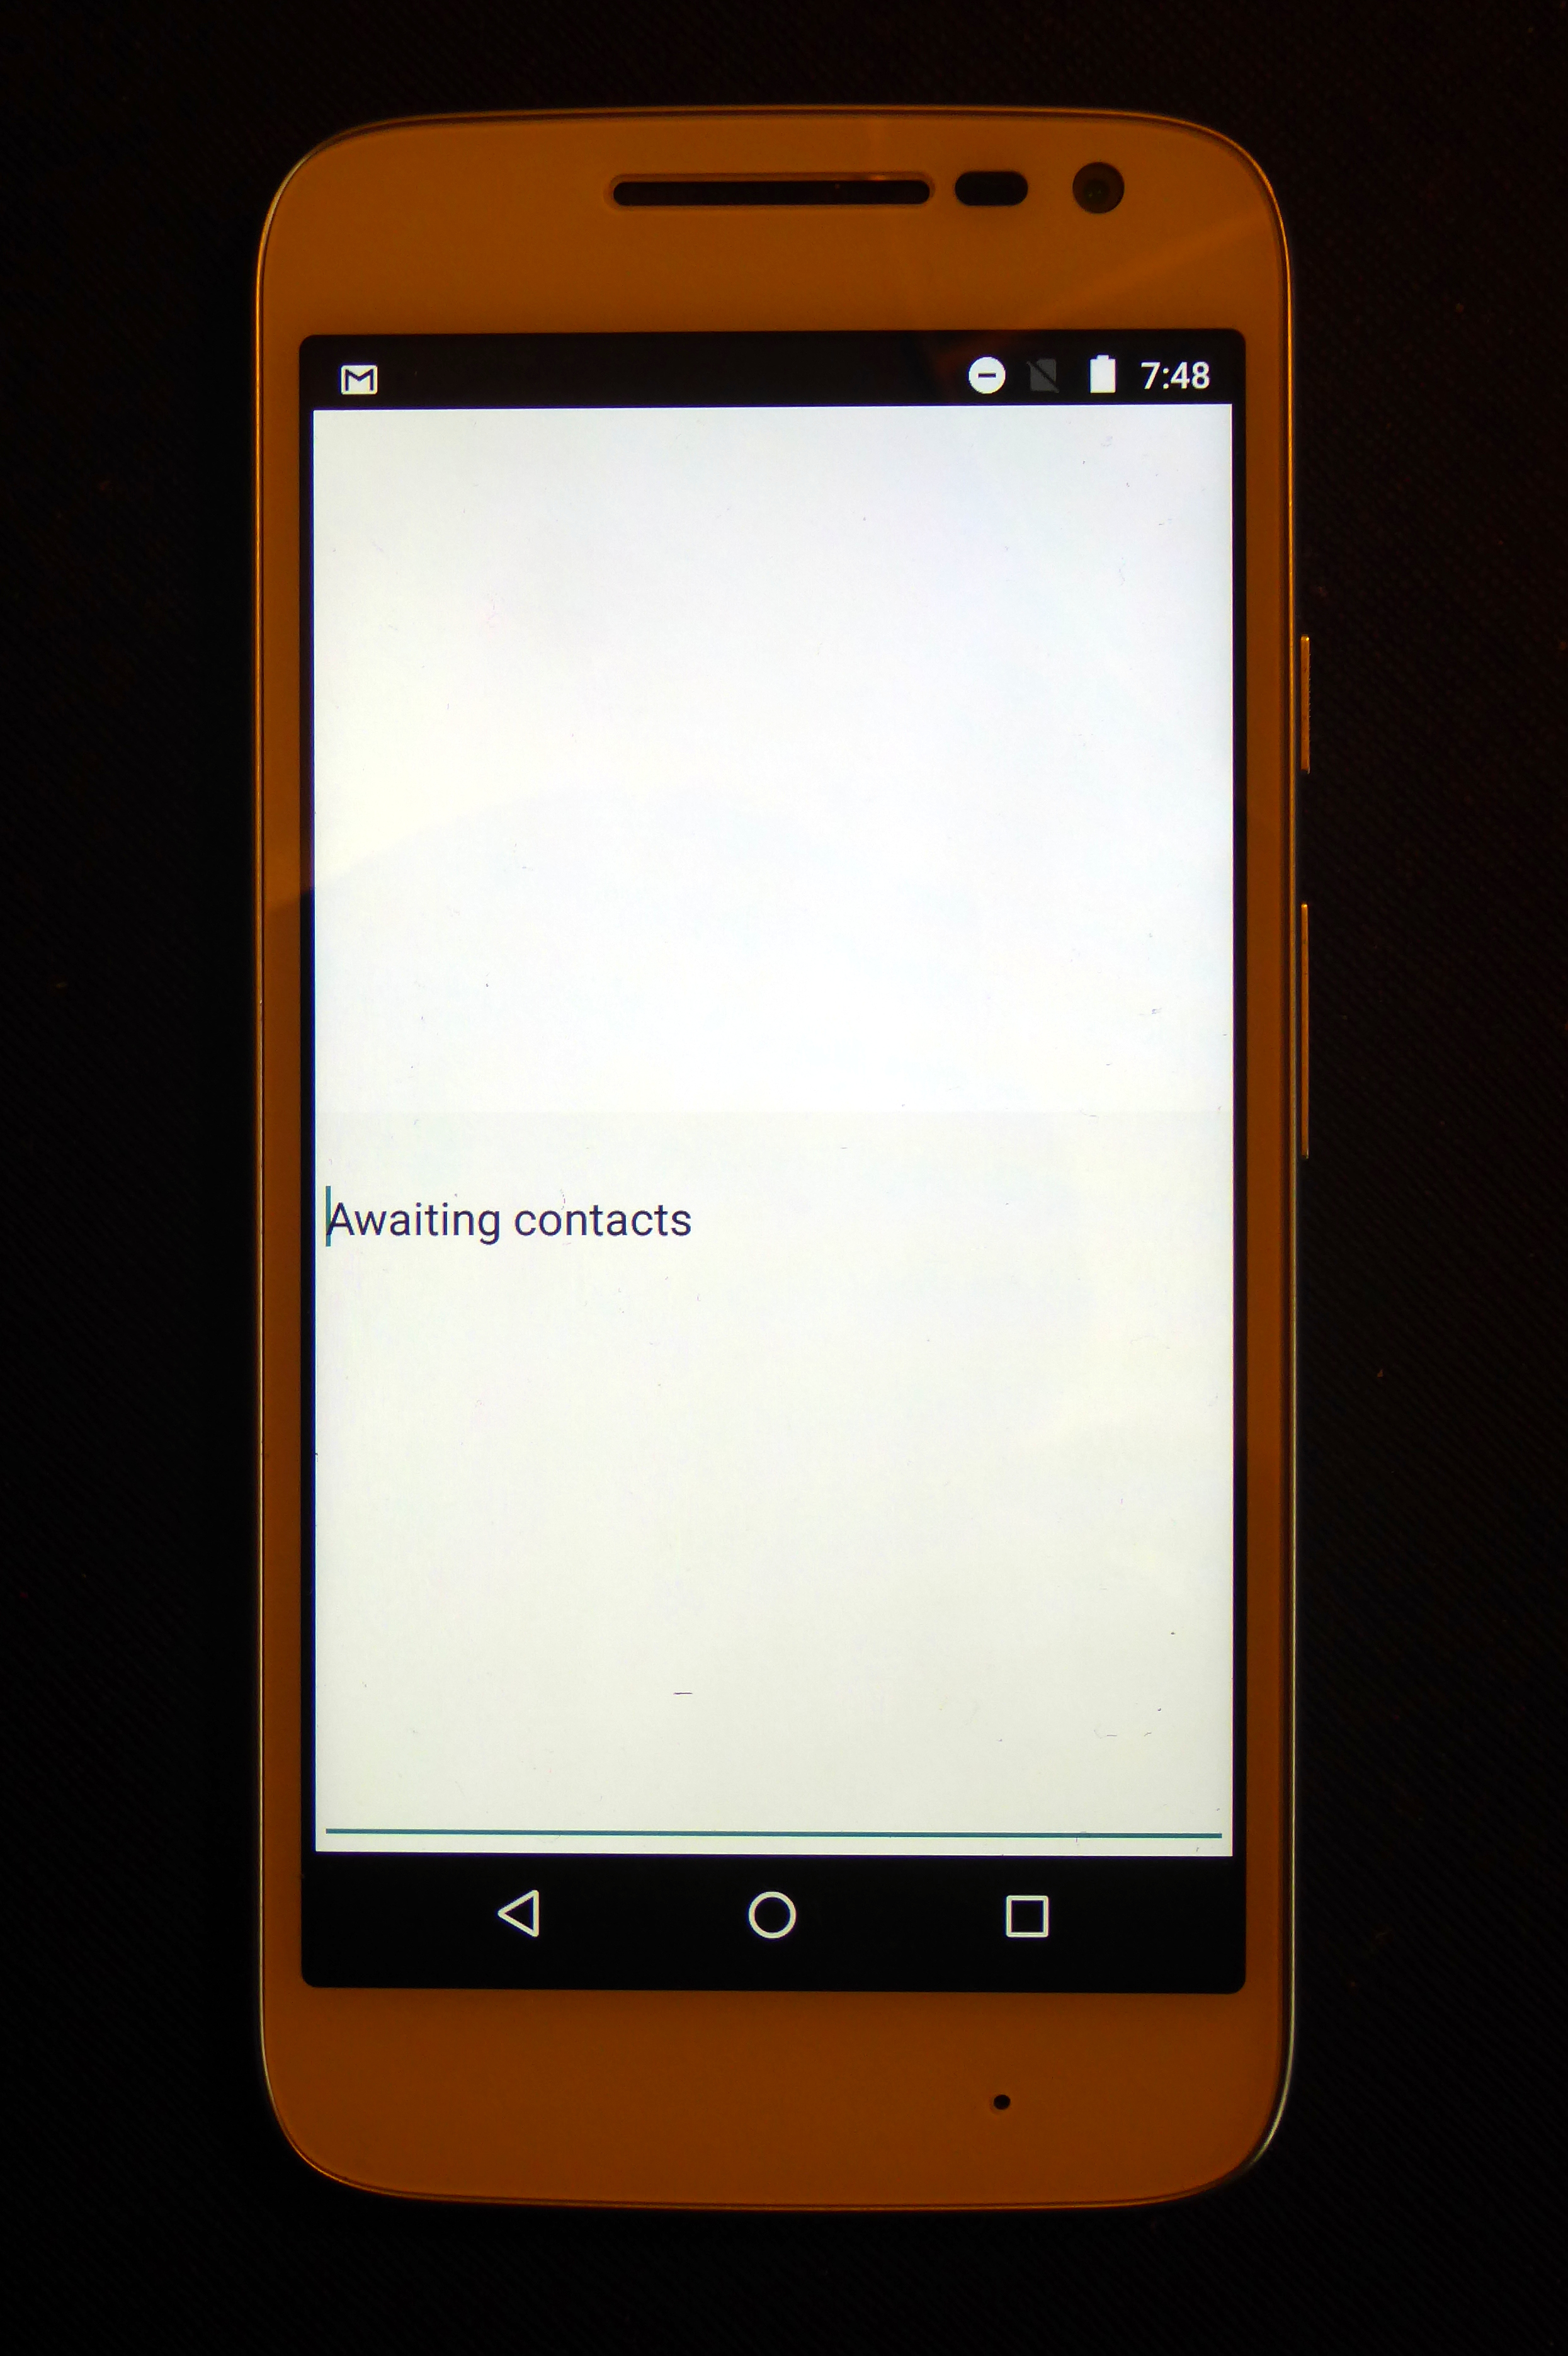
\includegraphics[height=0.45\textheight]{graphics/PhonePhotos/05 - PublisherBefore.jpg}
		\caption{Publisher Before Collusion}
		\label{fig:PublisherBefore}
	\end{subfigure}
\hfill	
	\begin{subfigure}{0.49\textwidth}
		\centering
		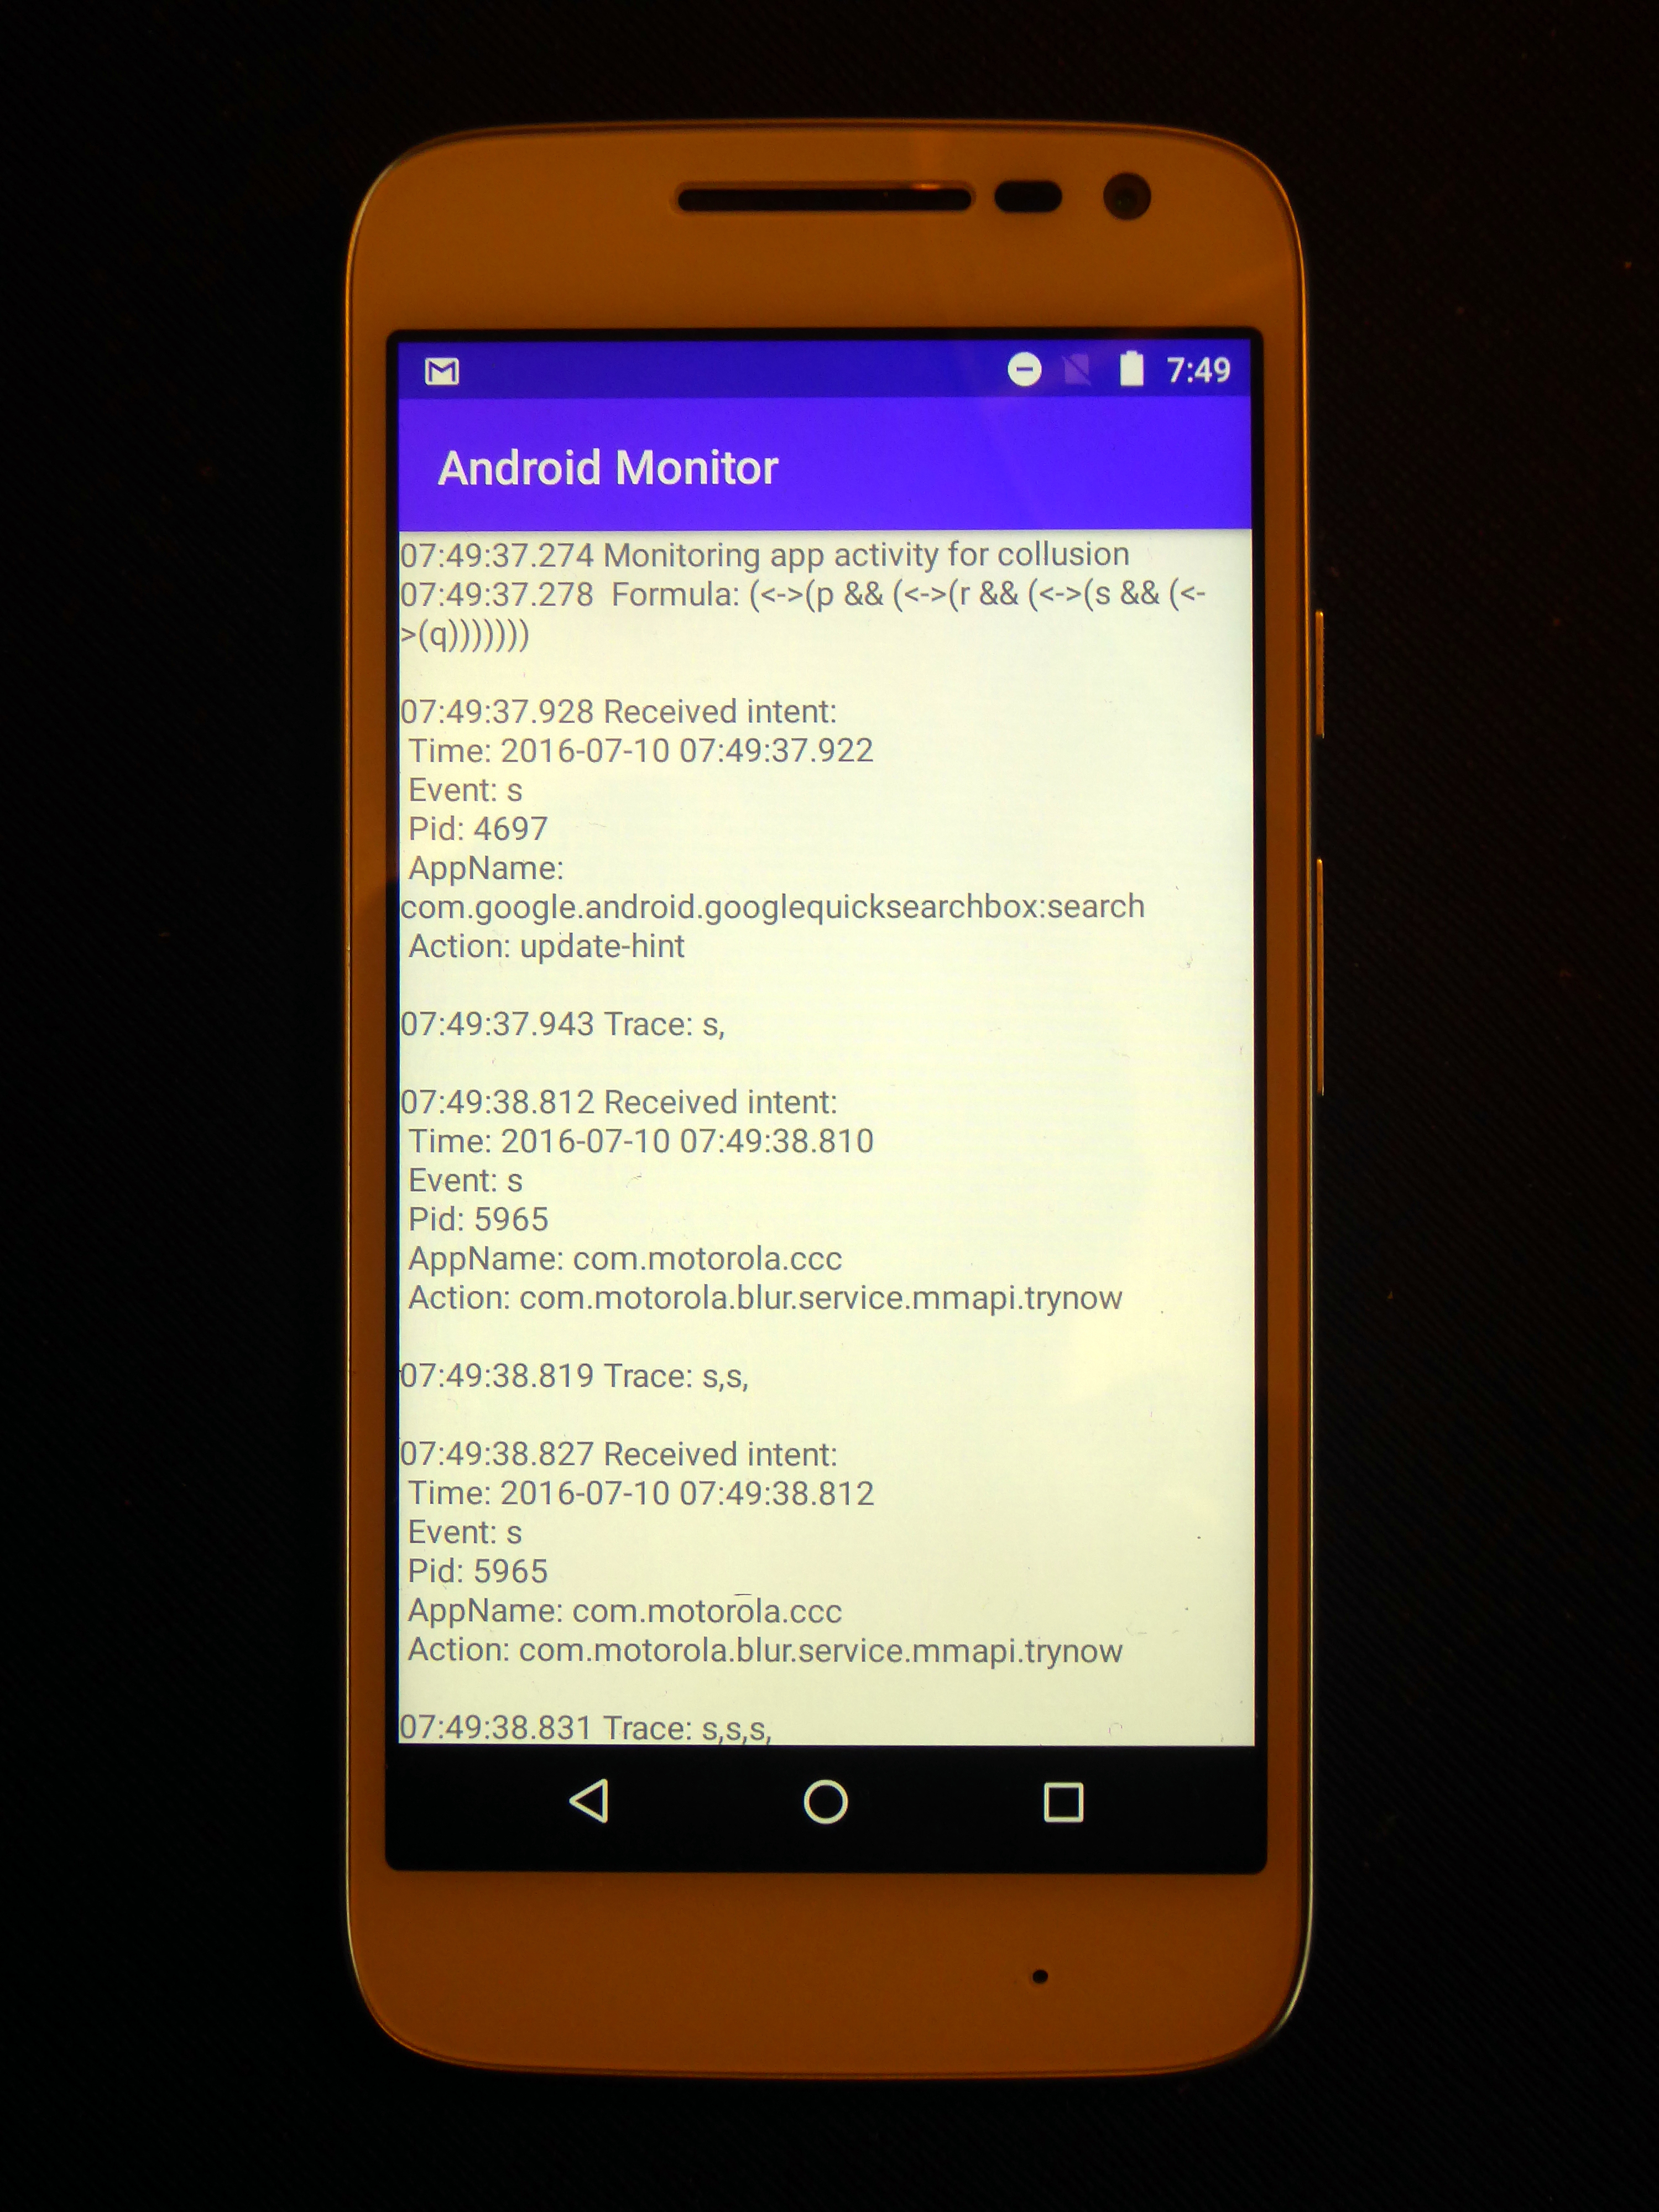
\includegraphics[height=0.45\textheight]{graphics/PhonePhotos/06 - MonitorBefore.jpg}
		\caption{Monitor Before Collusion}
		\label{fig:MonitorBefore}
	\end{subfigure}
\\
	\begin{subfigure}{0.49\textwidth}
		\centering
		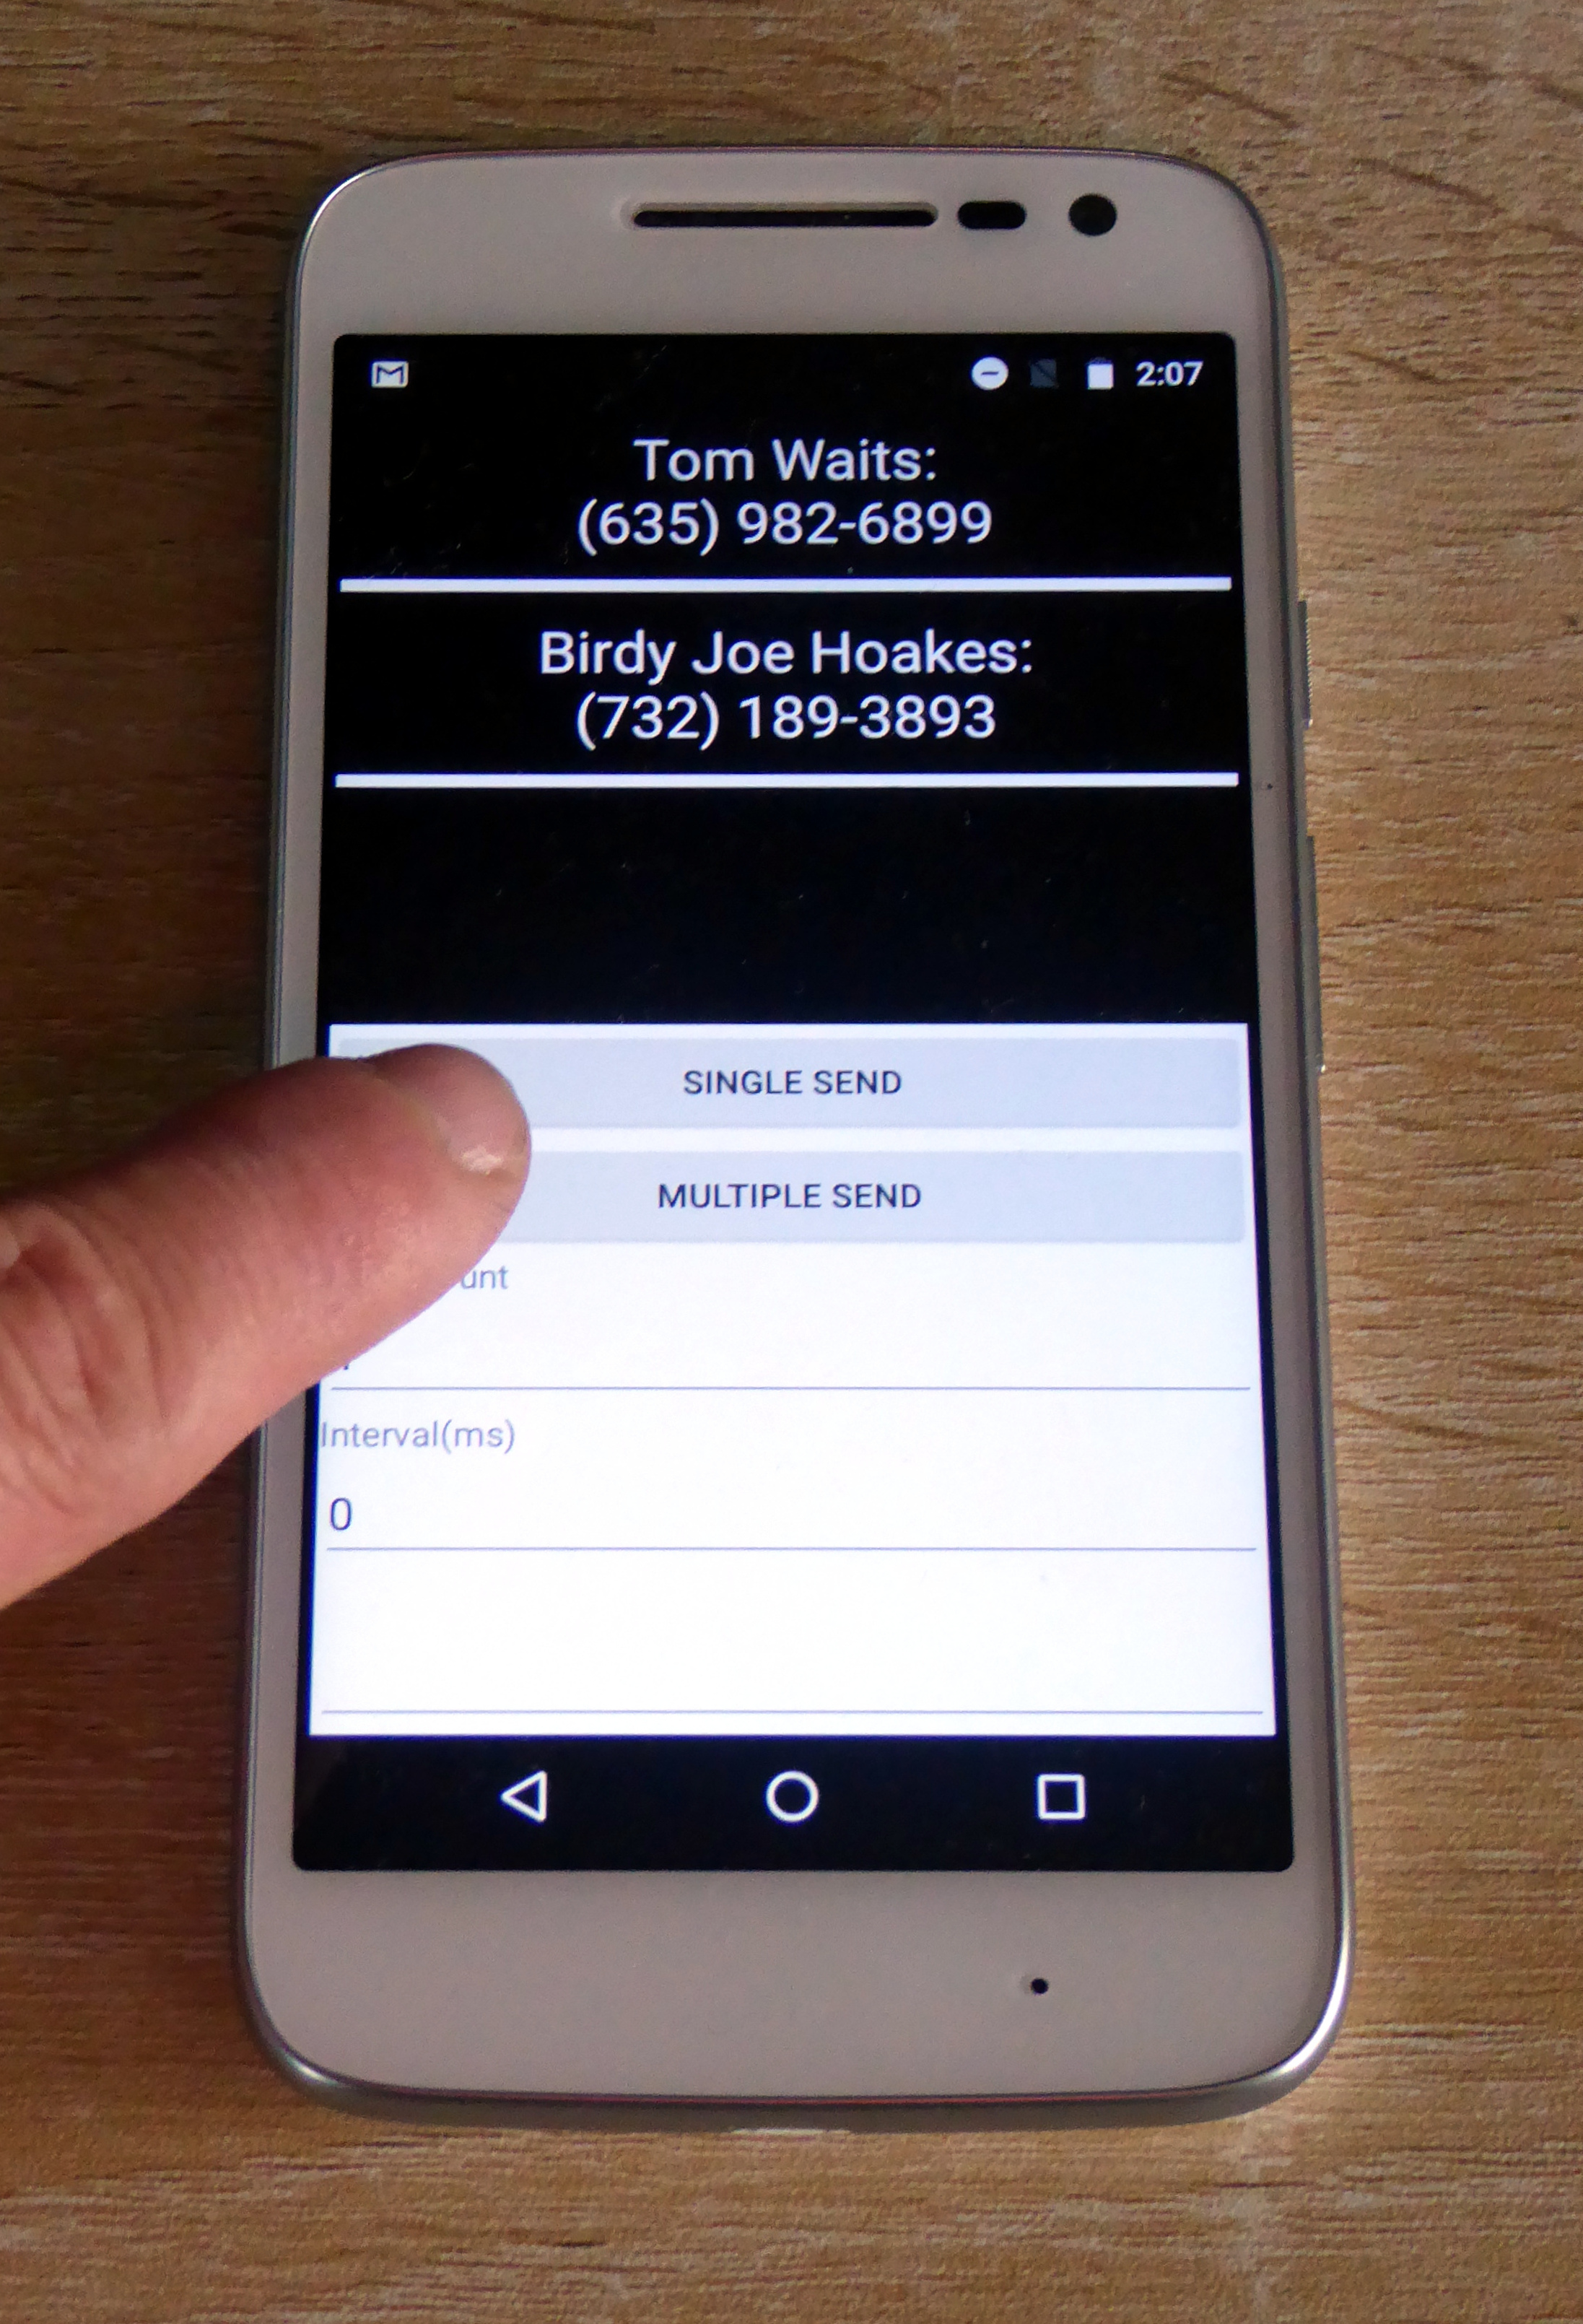
\includegraphics[height=0.45\textheight]{graphics/PhonePhotos/07 - ReaderSend.jpg}
		\caption{Reader Sending Contacts}
		\label{fig:ReaderSend}
	\end{subfigure}
	\caption{Before Collusion}
	\label{fig:BeforeCollusion}
\end{figure}

\newpage

\begin{figure}[h!]
	\centering
	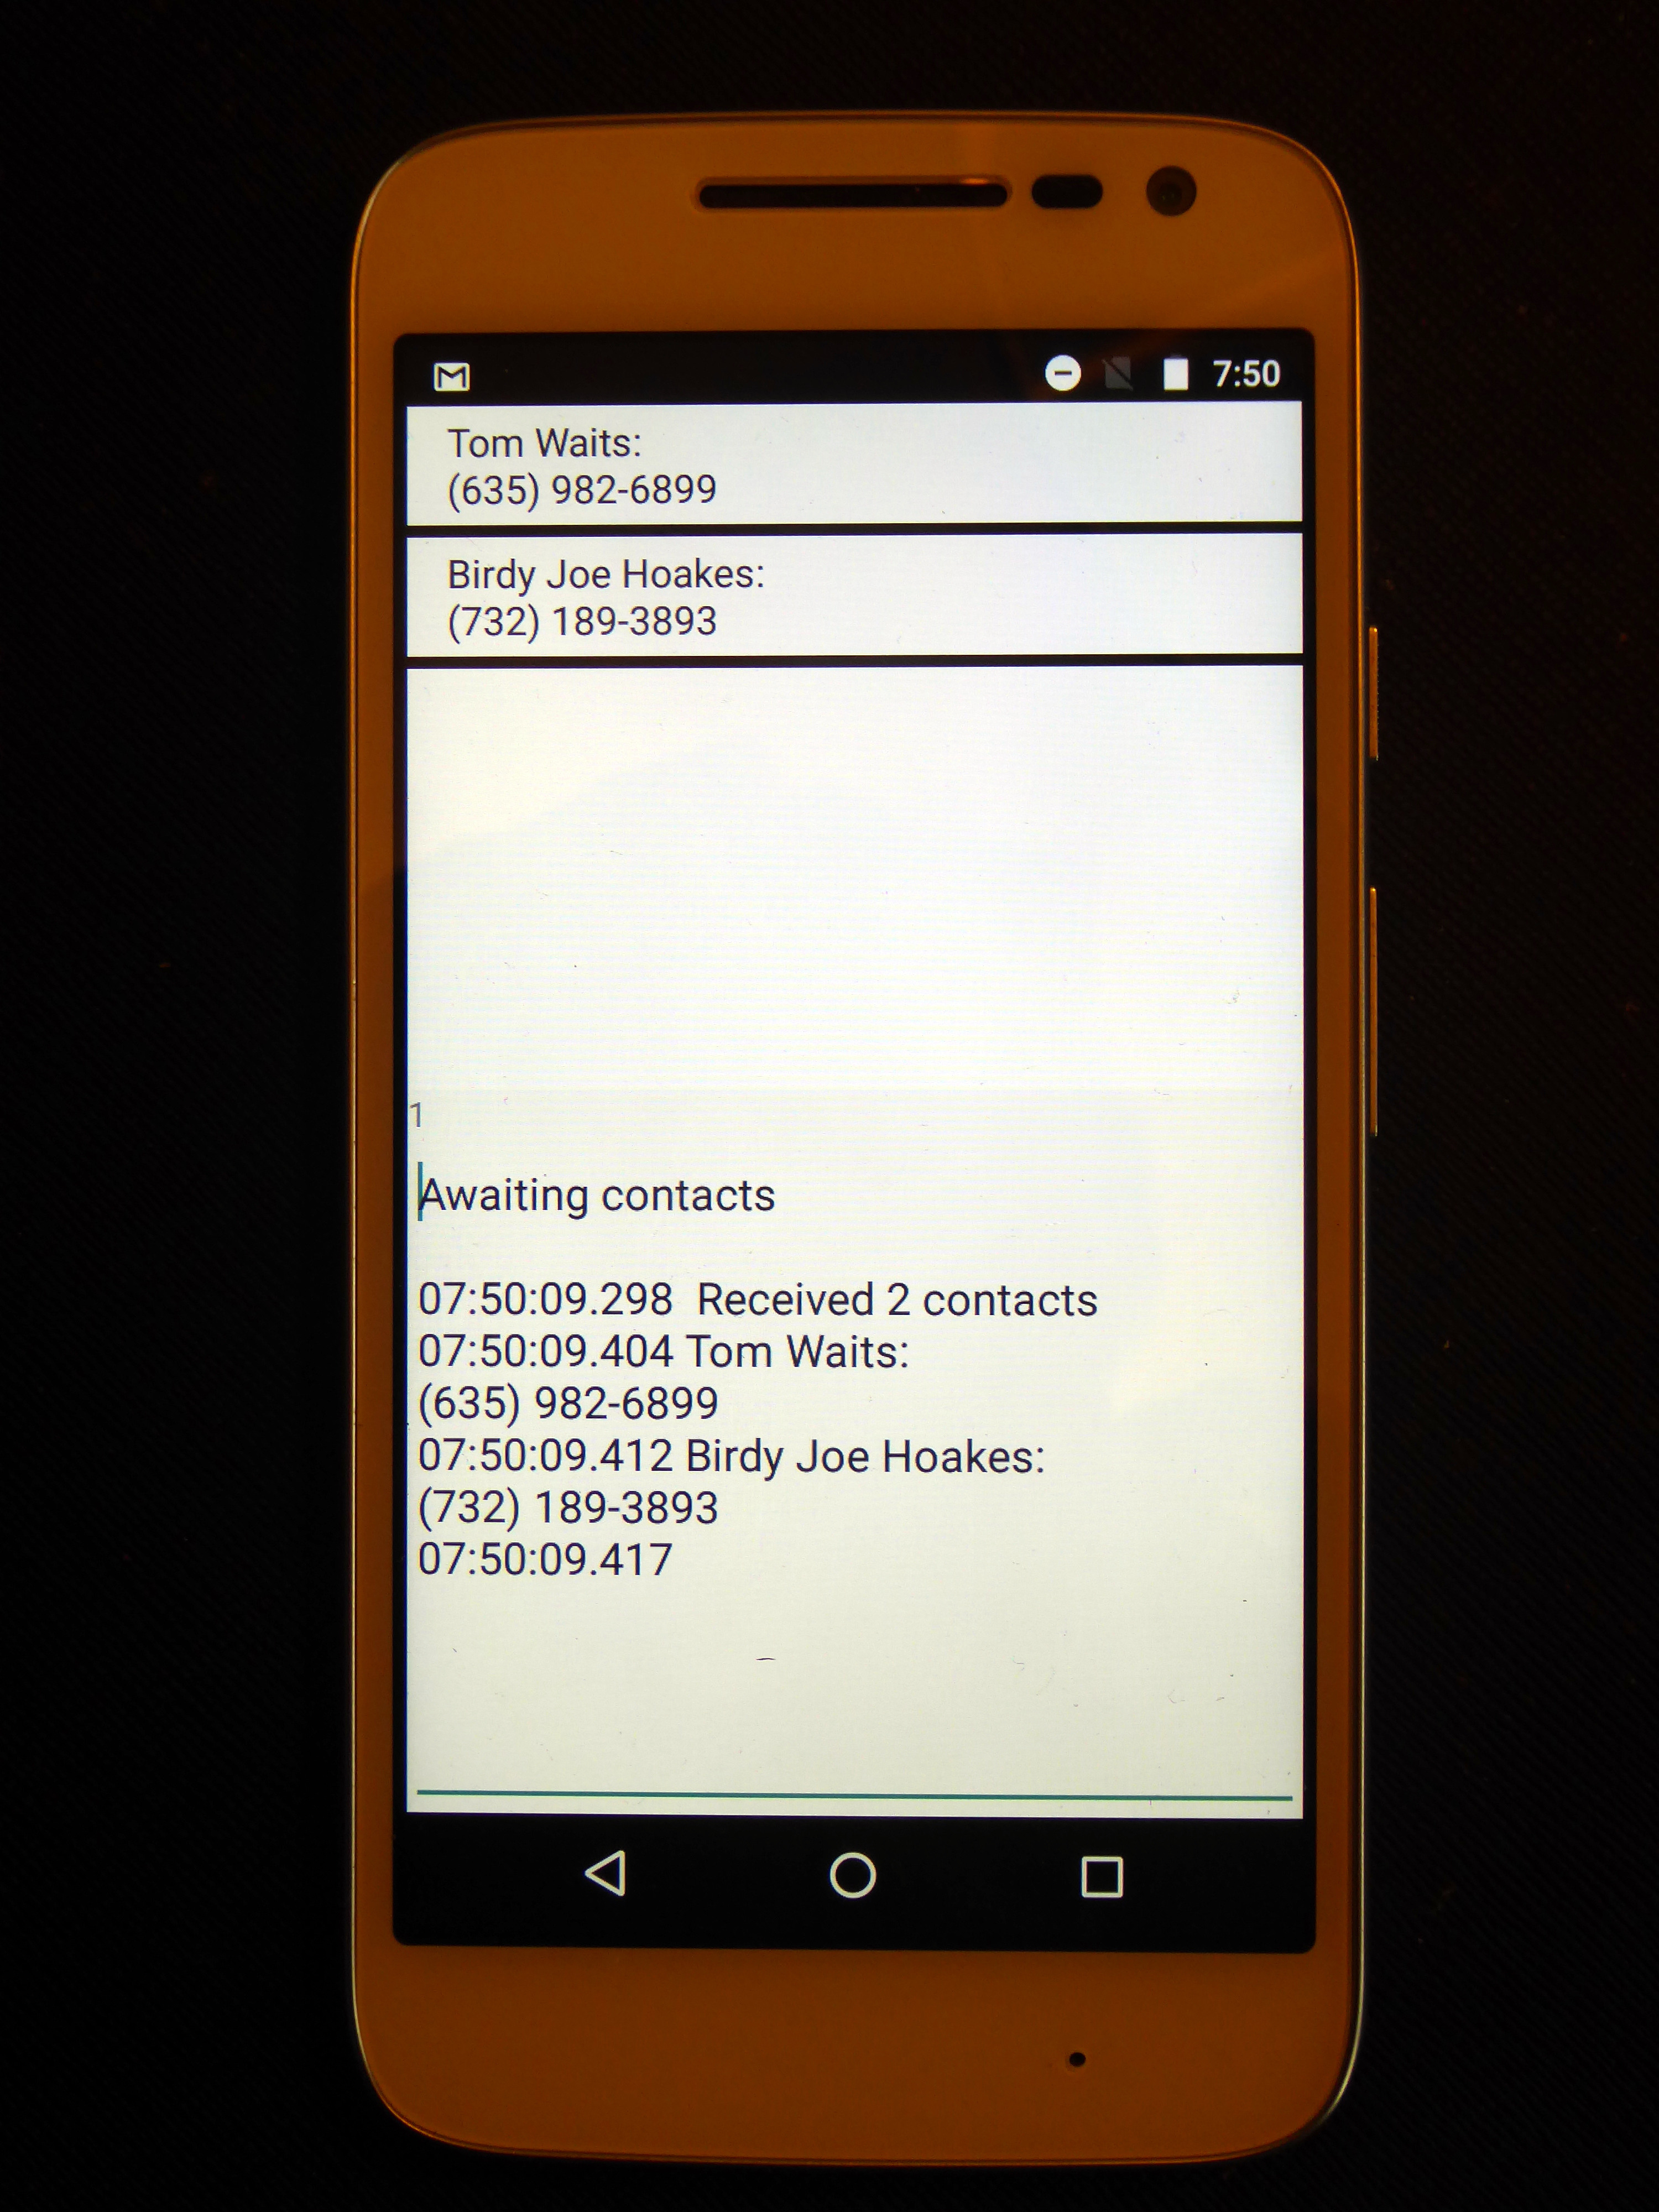
\includegraphics[width=0.7\linewidth]{graphics/PhonePhotos/08 - PublisherAfter.jpg}
	\caption{Publisher After Collusion}
	\label{fig:PublisherAfter}
\end{figure}

\newpage

\begin{figure}[h!]
   \centering
   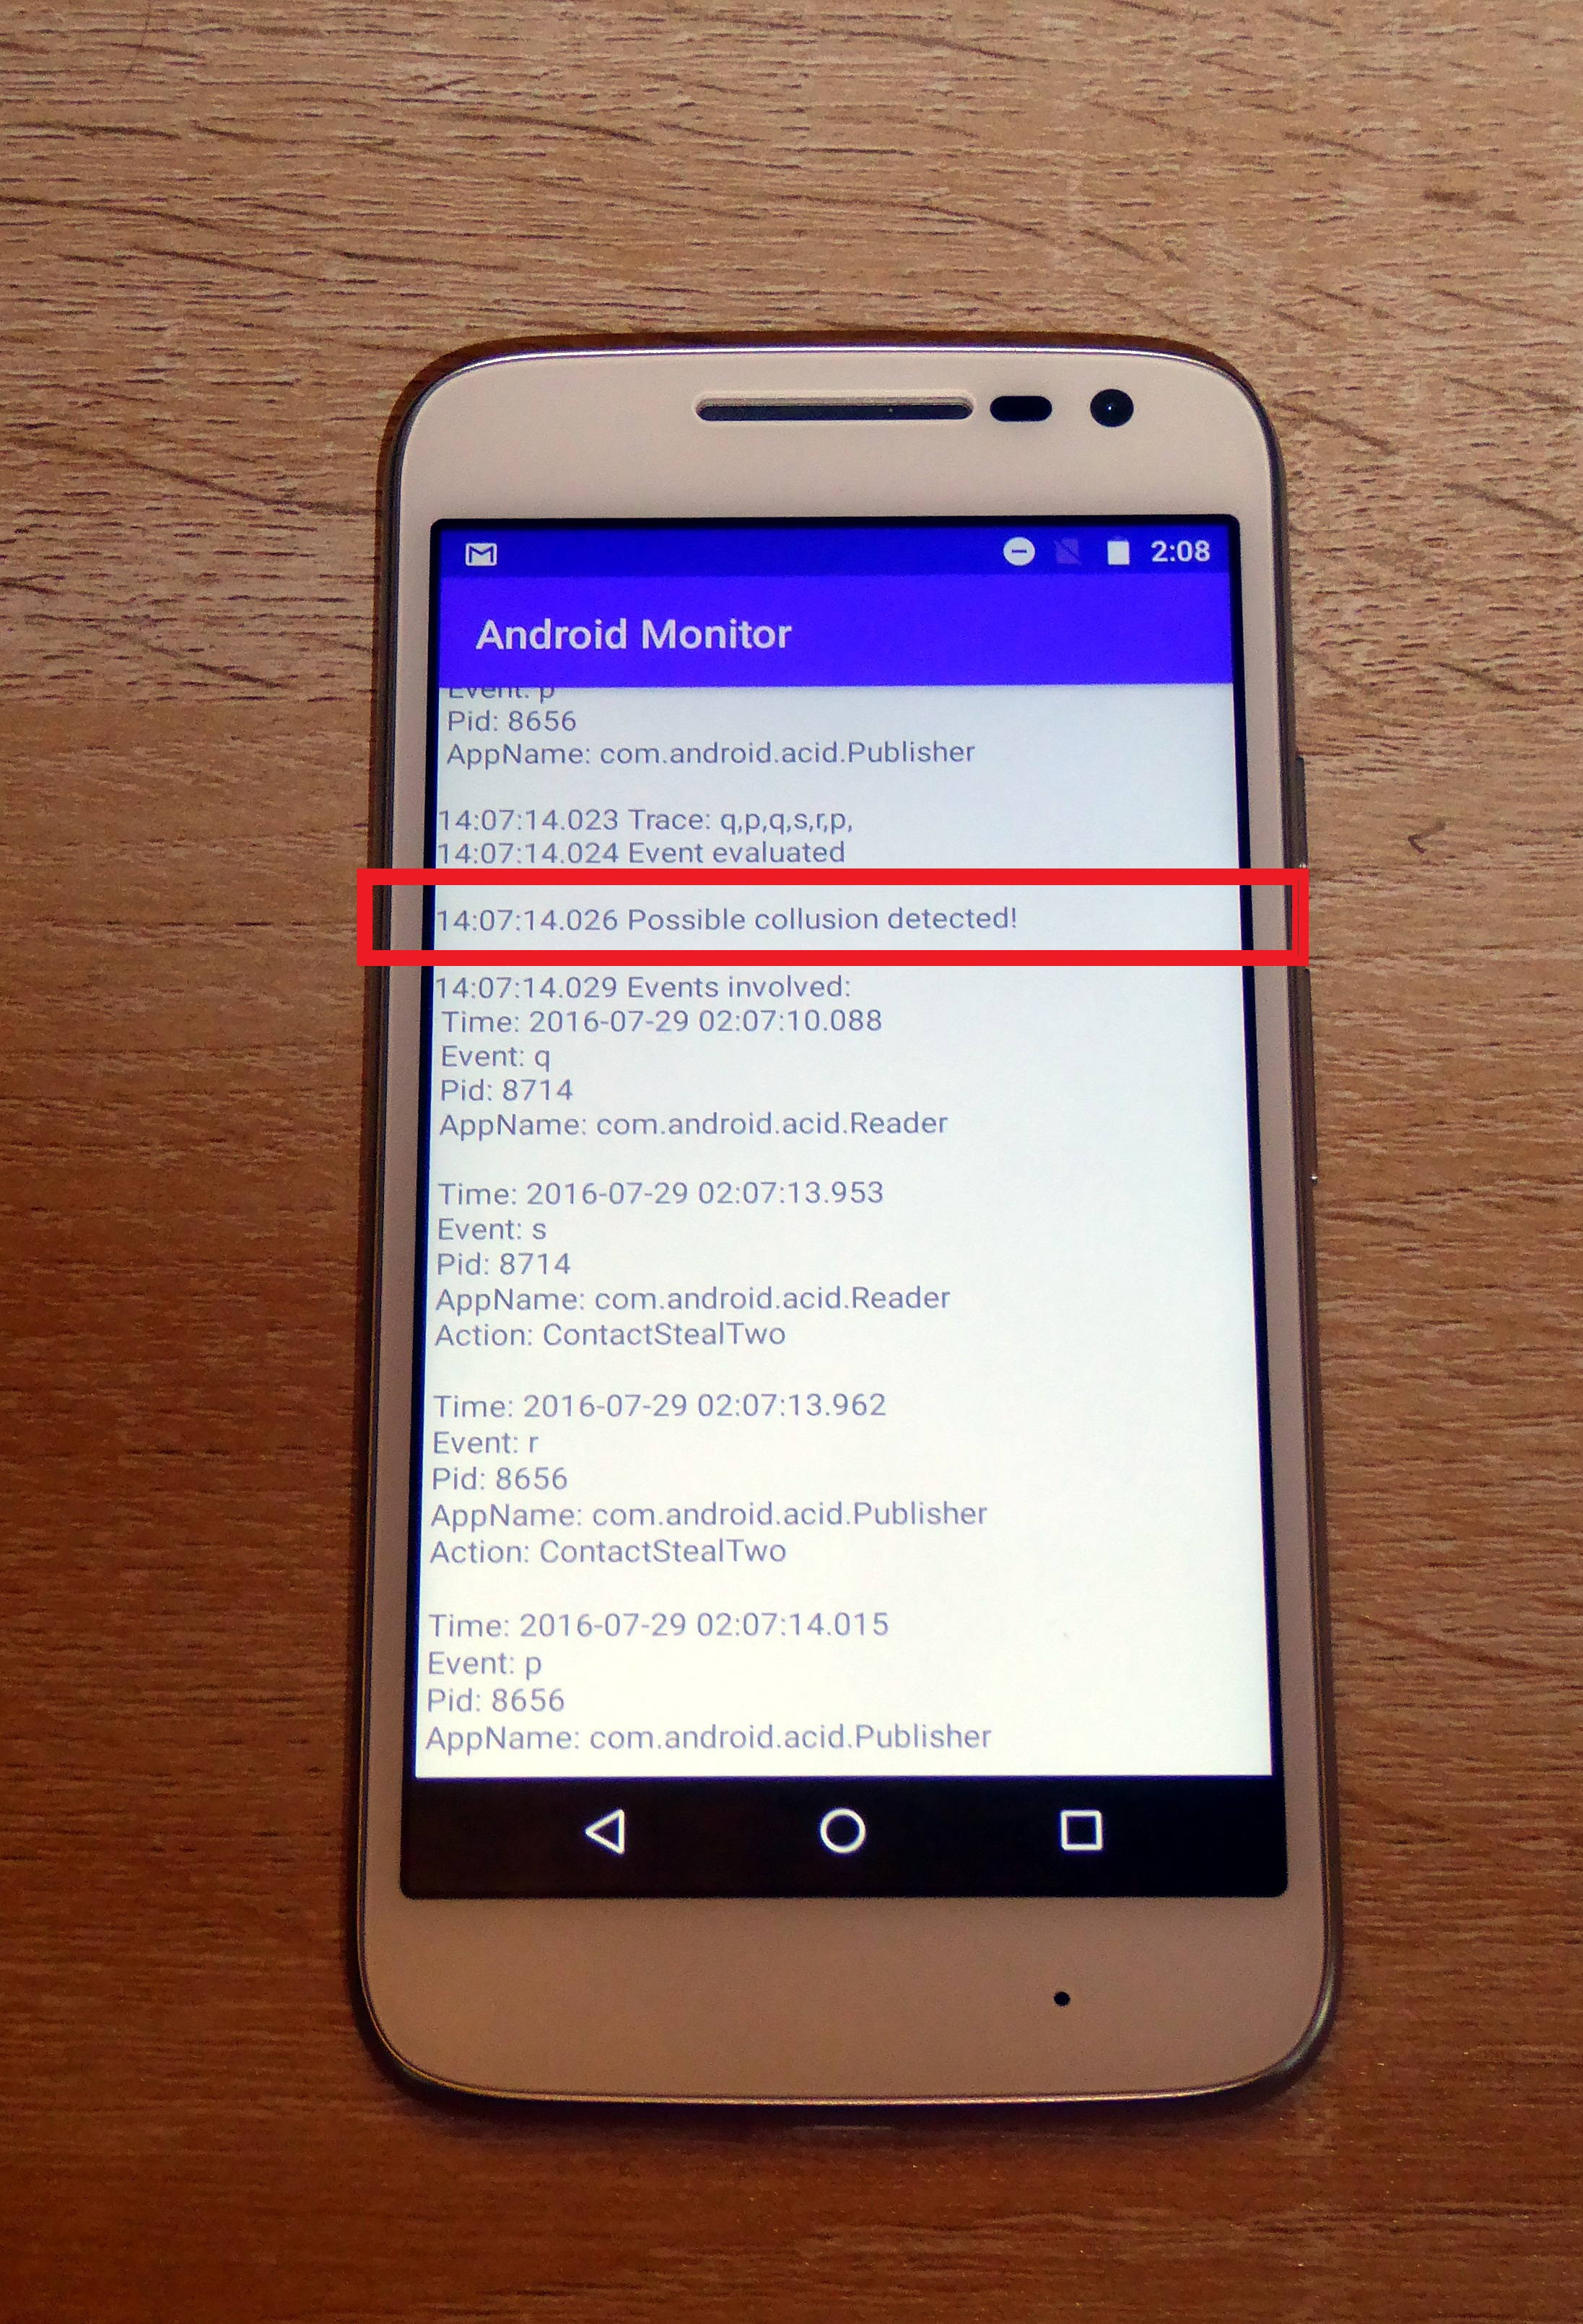
\includegraphics[width=0.7\linewidth]{graphics/PhonePhotos/09 - MonitorAfter.jpg}
   \caption{Monitor After Collusion}
   \label{fig:MonitorAfter}
\end{figure}

\newpage

\section{Subsequent Collusion Attacks}

After collusion has been detected, the monitor is reset so that it is able to detect further attacks.  Figure \ref{fig:SecondDetection} shows the monitor detecting a second attack that begins and ends after the first attack.

\begin{figure}[h!]
   \centering
   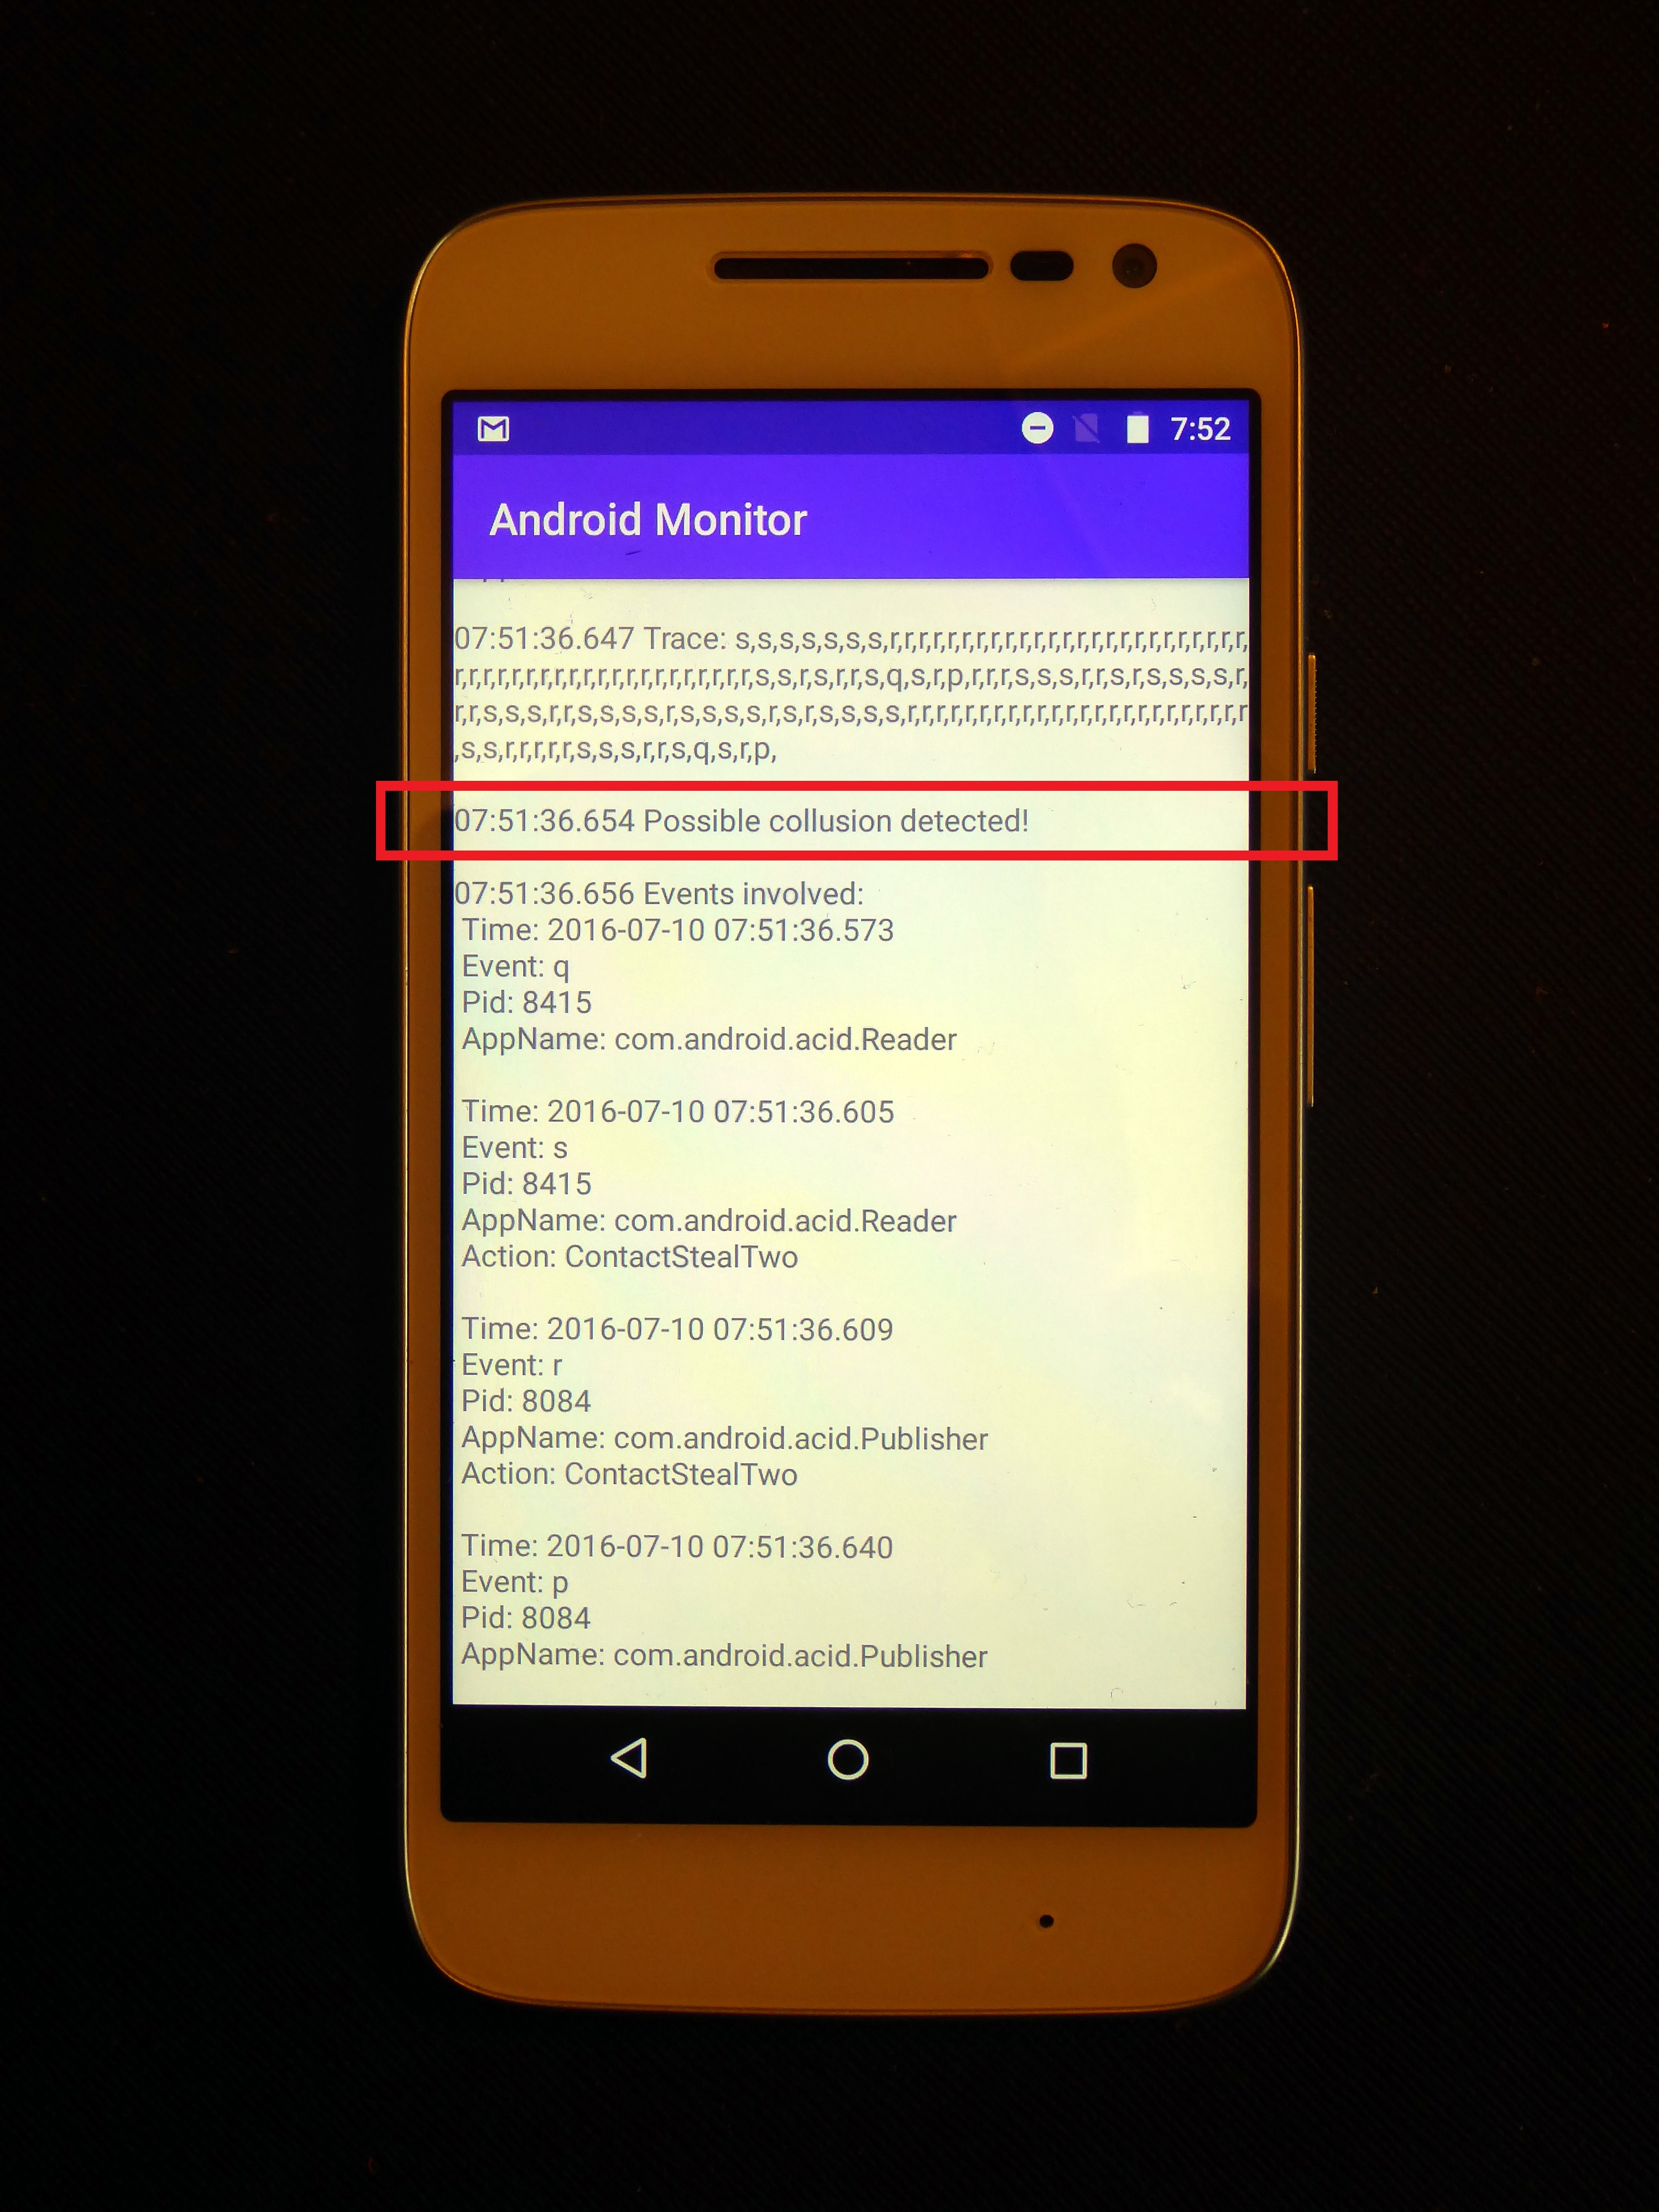
\includegraphics[width=0.7\linewidth]{graphics/PhonePhotos/10 - SecondDetection.jpg}
   \caption{Second Detection}
   \label{fig:SecondDetection}
\end{figure}

\newpage

\section{Negative Demonstration}

To illustrate the monitor operating among benign applications, we performed the same demonstration again but, the reader application was modified to not send the contacts it queried.  Doing this breaks the sequence of events required for a collusion attack because the reader will do nothing more than look at the contacts list.

\begin{wrapfigure}[26]{l}{0.6\linewidth}
	\centering
	\vspace{-12pt}
	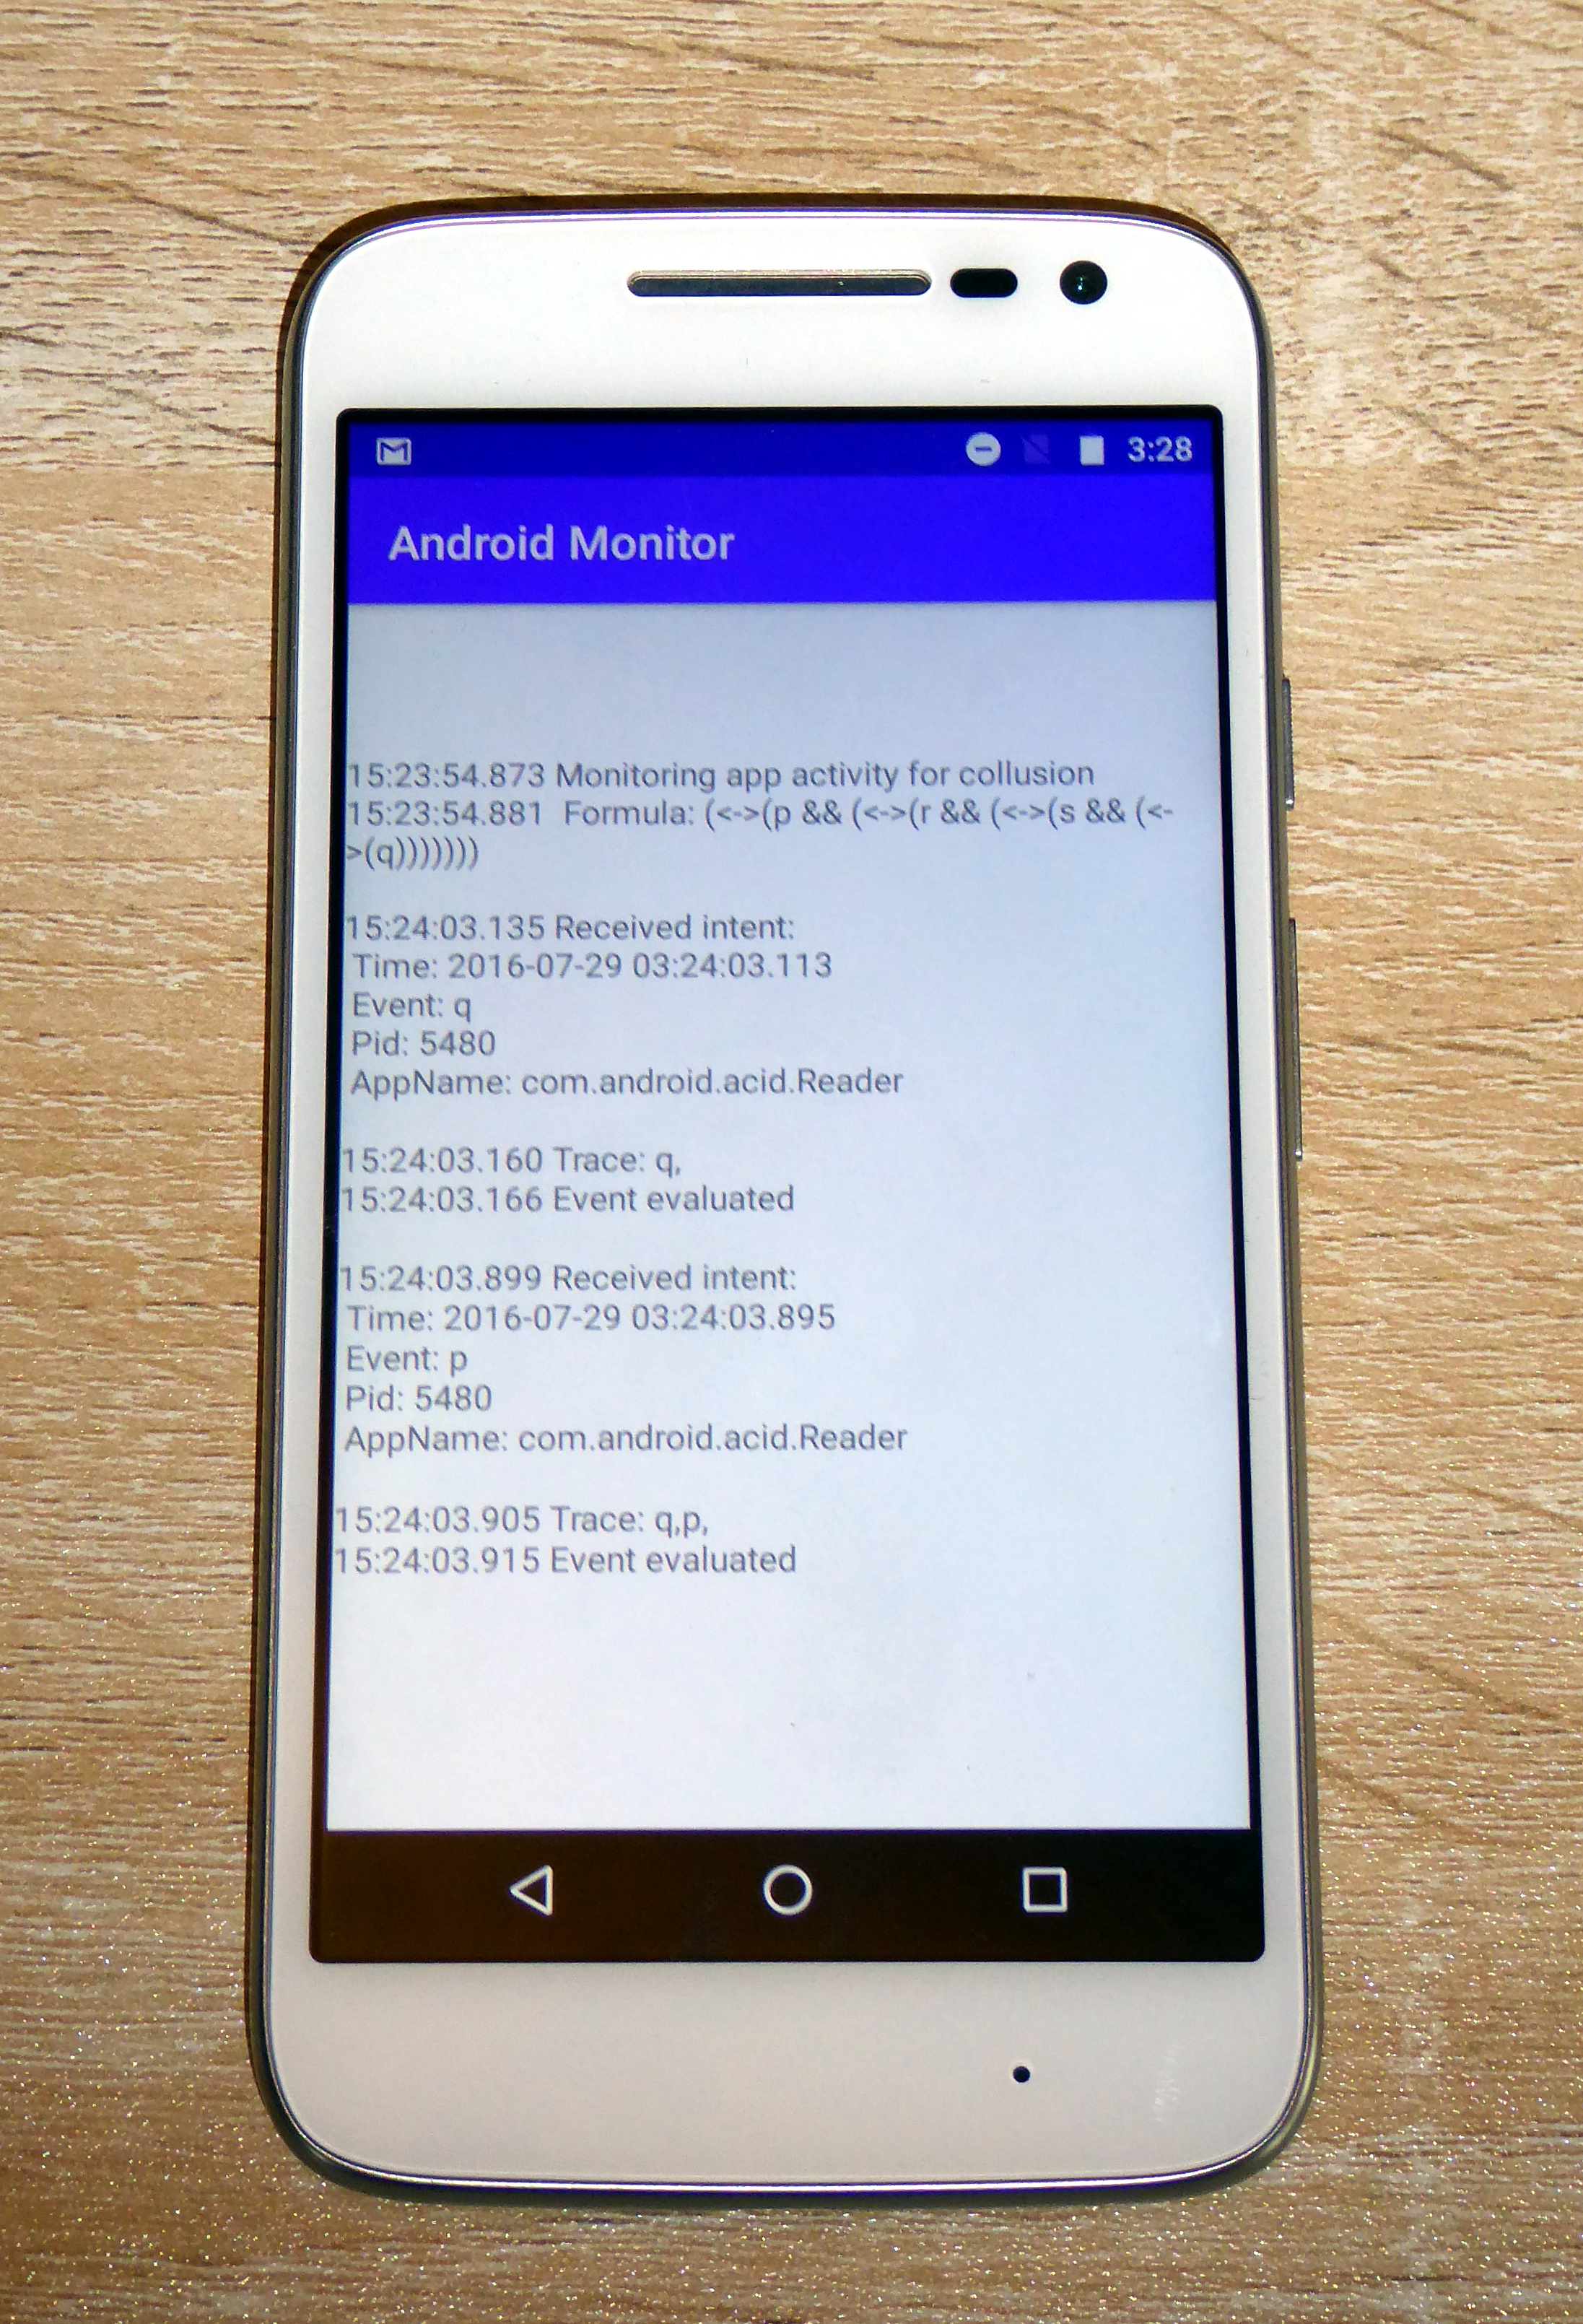
\includegraphics[width=0.58\textwidth]{graphics/PhonePhotos/11 - NegativeTest.jpg}
	\caption{Negative Demonstration}
	\label{fig:NegativeDemonstration}
\end{wrapfigure}

For brevity, Figure \ref{fig:NegativeDemonstration} shows only the monitor after the demonstration.  In the log, it can be seen that query and publish events both occurred, but there is no send event and, therefore, no receive.  The reader might be asking how did the monitor receive a publish event when the publisher app did not receive any contacts?  The log reveals the answer:  The publish event received by the monitor was performed by the reader application.  What happened is that after querying the contacts, the reader app displayed them on the screen.  It called the same method that the publisher app uses to display the contacts, thus, the interceptor noticed this and publish event was generated.  

Although the monitor received an intent to say the publish event occurred, neither the static, nor dynamic conditions were met.  Therefore, collusion was not detected.

\part{Conclusion}
\chapter{Summary}
\label{chap:Summary}

%6.  Make the summary short.  We fulfilled all our project aims - list them and reflect upon how well we have achieved them and why that are achived.  We have an app etc.

%We have found the original algorithm not to be suitable to realtime RV.  We have developed the RRH algorithm and shown that it is effective for realtime RV on android thanks to its constant monitoring time.  We have developed an app for runtime monitoring and instantiated it with a property for collusion detection of information theft and shown that it worked effectively.

In this chapter we reflect upon our original aims, what we did and how well we have achieved them.\\

\noindent
We began this project aiming to detect a security attack performed by colluding applications running on an Android device.  We wanted to detect the attack without modifying the applications under scrutiny, and the performance impact on the device should be minimal.  We decided the user doesn't need to enter their own security properties, and that the response to a security breach could be limited to recognition only.  Our question was whether we could use runtime verification to do this.

\GRKH\ presented a persuasive argument for constructing a monitor using their algorithm on the basis that it would meet our requirement for low computation cost when evaluating a security property.  On investigation, we found that the algorithm was only computationally light when evaluating a property over prerecorded traces.   When we attempted to use the algorithm in realtime, the computational cost increased at a quadratic rate with trace length.  Thus it was unsuitable for runtime verification in realtime.  But by modifying the algorithm, we overcame this.  We demonstrated that the \RRH\ algorithm is computationally light enough to be suitable for realtime use thanks to the constant evaluation time.

We developed a detection system around the \RRH\ algorithm that monitors application activity for the sequence of actions required to perform an attack.  The actions that provide the signature sequences are operating system calls made by applications involved in the attack.  A third-party framework applies a modification to the operating system that allows us to log these key operating system calls.  By working at the operating system level, we can monitor any application without changing it.  This is of utmost importance because it allows us to detect novel attacks by malicious applications developed after our monitor.\\

\noindent
Overall, we can effectively monitor for security threats on Android devices if some conditions are accepted:

\begin{itemize}

\item Runtime verification is effective at detecting malware if the threat utilises identifiable method calls in identifiable packages.  This includes documented operating system calls but could be calls from any known package.  We reason that many threats require the use of the O/S to access resources because Android runs on a diverse array of hardware and the O/S provides the only unified means to access resources.

\item Without a specification of the intent of software being scrutinised, the monitor will incur false positives.

\item If the monitor relies only on the satisfaction of an abstract LTL formula without considering the metadata associated with the events in the trace, then it can detect collusion sequences that span an infinite period.  However this will result in additional false positives.

\item Alternatively, if we wish to minimise false positives then the monitor must interrogate metadata associated with trace events.  Due to finite memory limitations it can only do this for collusion attempts that start and finish within a limited time frame.

\end{itemize}

%Limited time frame because of overlapping sequences.

%We remove complete sequences from the log but incomplete must stay indefinitely.  We have limited memory so we have to remove the earliest part of the log eventually.  If a sequence spans longer than this period we will not recognises it.
\chapter{Future Work}
\label{chap:Future Work}

In this chapter we look into which directions we can take this research in the medium term, what future research into Android security and runtime verification has been enabled thanks to the progress made here, and what progress is enabled in computer science. \\

\noindent
In the medium term, say with a further six months of research, we would concentrate on three areas:

\begin{enumerate}
\item Conduct systematic experimentation with the monitor to investigate if we can detect at least part of the Pegasus malware.  An organisation called Lookout directed research into the inner workings of Pegasus on Android \cite{PegasusOnAndroid}.  They discovered that Pegasus makes use of several operating system calls, and the parameters are hardcoded.  We can intercept and log these calls, and therefore we have good reason to assume we could detect Pegasus.

\item Extend the LTL grammar and semantics so properties can be formulated from an unspecified number of colluding applications.

\item Concerning the technical implementation of the monitor, we would seek to cover the latest Android versions, integrate the function of the Xposed framework into the monitor and provide a fully-fledged security monitoring app.
\end{enumerate}

\noindent
Beyond six months, the project has raised some questions in the field of runtime verification that open opportunities for deeper investigations:

Can our technique for deriving monitors for concrete events from monitors for abstract events yields better results than using monitors derived from LTLFO (first-order linear temporal logic)?

When we implemented the \RH\ algorithm in chapter \ref{chap:Runtime Verification with the Rosu-Havelund Algorithm}, we learned that the fundamental problem when evaluating future operators is not knowing what a future event will be.  The algorithm is unsuitable for realtime use because it must evaluate the trace from the latest event to the earliest, which raises complexity.  There is a range of different paths of research into this problem:

The solution we presented here is to formulate properties with past operators and reverse the order of evaluation. To back this up, in chapter \ref{chap:Reverse Rosu-Havelund Algorithm} we made the conjecture that: Any security property we wish to formulate can be written in terms of past events and past operators.  We would start by examining the relationship between future and past LTL operators an attempt to confirm the conjecture.

Next, there is an opportunity to explore whether we can combine forward and reverse evaluation into a single algorithm capable of evaluating both past and future operators.  While it is likely possible, we expect it will still be unsuitable for realtime use when future operators are employed.

The greatest advancement might be to adapt the algorithm to use a three-valued variation of LTL, similar to the logic Bauer et al. described in their paper Runtime Verification for LTL and TLTL \cite{RVForLTLAndTLTL}.  The LTL they use includes a logical value for unknown.  After all, when evaluating future operators, it appears that unknown future events are precisely what we are dealing with.\\
\\
\noindent
In the broader field of computer science, the development of the \RRH\ algorithm has brought progress.  We now have a general algorithm for constructing monitors that evaluate past logic propositional LTL formulae in realtime.  This brings new possibilities for investigating monitoring in the fields of safety and security.\\
\\
\noindent
We are aware that alongside the main CPU that runs Android, a mobile device has a baseband modem that implements mobile network and WiFi connectivity.  The issue is that the baseband modem is a System-on-Chip (SoC) device with its own processor.  The processor has direct hardware access to all the network connectivity features implemented by the baseband modem without going through Android.  The significance is that none of the Android security features have any influence over the baseband modem.  Our monitor observes Android activity on the main CPU, but the baseband modem can run programs that communicate outside the device without even informing Android.  Zero-click attacks on the baseband modem have been performed by sending an SMS containing malicious code to the mobile device.  The baseband modem receives the SMS first and the code is run by the SoC.  Although we have been monitoring Android applications, we believe there is value in investigating if it is possible to monitor the baseband modem.

%Bibliography
\bibliography{bibliography}

%Table Of Contents
\addtocontents{toc}{\protect\setcounter{tocdepth}{-1}}

%Appendices
\appendix
\newgeometry{left=1cm,bottom=0.1cm, top = 2cm}
\chapter{Source Code}
\label{app:Code}

All the source code developed in this project is available in a public repository on GitHub.  The following sections list where to find the code and details of the development environment required to build the code.

\section{\RH\ Test Harness}
\label{app:RHCode}

The standard \RH\ algorithm is written in Java and built using the Eclipse IDE, version: 2020-09 (4.17.0).  The source code for the standard \RH\ implementation is here:\\
\\
\noindent \url{https://github.com/RichardJohnAllen/RuntimeVerificationForAndroidSecurity/tree/main/Eclipse/RosuHavelund\%20-\%20Standard}

\section{\RRH\ Test Harness}
\label{app:RRHCode}

The \RRH\ algorithm is written in Java and built using the Eclipse IDE, version: 2020-09 (4.17.0).  The source code for the \RRH\ implementation is here:\\
\\
\noindent \url{https://github.com/RichardJohnAllen/RuntimeVerificationForAndroidSecurity/tree/main/Eclipse/ReverseRosuHavelund}

\section{Performance Test Code}
\label{app:PerformanceTestCode}

Performance tests were executed using two applications that were developed to stage a collusion attack at will.  The two applications are called the Reader and the Publisher.  Both applications are modified versions of applications developed by Callum Dicker \cite{Dicker}.  There were developed in Java using the Android Studio IDE, version: 4.1.3.\\
\\
\noindent The Reader app can be found here:\\
\noindent \url{https://github.com/RichardJohnAllen/RuntimeVerificationForAndroidSecurity/tree/main/AndroidStudio/Reader}\\
\\
\noindent The Publisher app can be found here:\\
\noindent \url{https://github.com/RichardJohnAllen/RuntimeVerificationForAndroidSecurity/tree/main/AndroidStudio/Publisher}\\

%\newpage

\section{Interceptor Code}
\label{app:InterceptorCode}

The same Interceptor Xposed module is used for the standard \RH\ monitor and the\\
\RRH\ monitor.  The source code is written in Java using Android Studio, version: 4.1.3.\\
\\
\noindent The source code of the Interceptor is here:\\
\noindent \url{https://github.com/RichardJohnAllen/RuntimeVerificationForAndroidSecurity/tree/main/AndroidStudio/AndroidInterceptor}

\section{Standard \RH\ Monitor Code}
\label{app:StandardRHMonitorCode}

The source code for the standard \RH\ Monitor application is written in Java using Android Studio, version: 4.1.3.\\
\\
\noindent The source code of the Monitor is here:\\
\noindent \url{https://github.com/RichardJohnAllen/RuntimeVerificationForAndroidSecurity/tree/main/AndroidStudio/AndroidMonitor\%20-\%20Standard}

\section{\RRH\ Monitor Code}
\label{app:MonitorCode}

The source code for the \RRH\ Monitor application is written in Java using Android Studio, version: 4.1.3.\\
\\
\noindent The source code of the Monitor is here:\\
\noindent \url{https://github.com/RichardJohnAllen/RuntimeVerificationForAndroidSecurity/tree/main/AndroidStudio/AndroidMonitor}

\section{Development Environments}

\noindent Eclipse can be downloaded here:\\
\noindent \url{https://www.eclipse.org/downloads/}\\

\noindent Android Studio can be downloaded here:\\
\noindent \url{https://developer.android.com/studio#downloads}\\

\chapter{\RH\ Functional Test Cases}
\label{app:RHFunctionalTestCases}

\begin{table}[h!]
	\centering
	\begin{tabular}{l r}
		\begin{tabular}{c|c} 
		Operator & Formula\\
		\hline
		NEXT & $ (N(b)) $\\
		\hline
		Trace & Expected Result \\
		\hline\hline
		$ \langle \rangle $ & False \\
		$ \langle a \rangle $ & False \\
		$ \langle b \rangle $ & False \\
		$ \langle a,a \rangle $ & False \\
		$ \langle a,b \rangle $ & True \\
		$ \langle b,a \rangle $ & False \\
		$ \langle b,b \rangle $ & True \\
		\hline
		\end{tabular}
	&
		\begin{tabular}{c|c} 
		Operator & Formula\\
		\hline
		NOT & $ (!a) $\\
		\hline
		Trace & Expected Result \\
		\hline\hline
		$ \langle \rangle $ & True \\
		$ \langle a \rangle $ & False \\
		$ \langle b \rangle $ & True \\
		\hline
		\end{tabular}
	\end{tabular}
	\caption{Operator Functional Tests}
	\label{tab:OperatorFunctionalTests}
\end{table}

\begin{table}[h!]
	\centering
	\begin{tabular}{l c r}
		\begin{tabular}{c|c} 
		Operator & Formula\\
		\hline
		ALWAYS & $ (<>(a)) $\\
		\hline
		Trace & Expected Result \\
		\hline\hline
		$ \langle \rangle $ & False \\
		$ \langle a \rangle $ & True \\
		$ \langle b \rangle $ & False \\
		$ \langle a,a \rangle $ & True \\
		$ \langle a,b \rangle $ & False \\
		$ \langle b,a \rangle $ & False\\
		$ \langle b,b \rangle $ & False \\
		\hline
		\end{tabular}
	&
		\begin{tabular}{c|c} 
		Operator & Formula\\
		\hline
		EVENTUALLY & $ ([](a)) $\\
		\hline
		Trace & Expected Result \\
		\hline\hline
		$ \langle \rangle $ & False \\
		$ \langle a \rangle $ & True \\
		$ \langle b \rangle $ & False \\
		$ \langle a,a \rangle $ & False \\
		$ \langle a,b \rangle $ & True \\
		$ \langle b,a \rangle $ & True \\
		$ \langle b,b \rangle $ & False \\
		\hline
		\end{tabular}
	&
		\begin{tabular}{c|c} 
		Operator & Formula\\
		\hline
		IMPLIES & $ (a\ \ \texttt{=>} (<>(b))) $\\
		\hline
		Trace & Expected Result \\
		\hline\hline
		$ \langle \rangle $ & True \\
		$ \langle a \rangle $ & False \\
		$ \langle b \rangle $ & True \\
		$ \langle a,a \rangle $ & False \\
		$ \langle a,b \rangle $ & True \\
		$ \langle b,a \rangle $ & True \\
		$ \langle b,b \rangle $ & True \\
		\hline
		\end{tabular}
	\end{tabular}
	\caption{Operator Functional Tests continued}
	\label{tab:OperatorFunctionalTestsContinued}
\end{table}		

\begin{table}[h!]
	\centering
	\begin{tabular}{l c r}
		\begin{tabular}{c|c} 
		Operator & Formula\\
		\hline
		AND & $ (a\ \&\&\ (<>(b))) $\\
		\hline
		Trace & Expected Result \\
		\hline\hline
		$ \langle \rangle $ & False \\
		$ \langle a \rangle $ & False \\
		$ \langle b \rangle $ & False \\
		$ \langle a,a \rangle $ & False \\
		$ \langle a,b \rangle $ & True \\
		$ \langle b,a \rangle $ & False \\
		$ \langle b,b \rangle $ & False \\
		\hline
		\end{tabular}
	&
		\begin{tabular}{c|c} 
		Operator & Formula\\
		\hline
		OR & $ (a\ ||\ b) $\\
		\hline
		Trace & Expected Result \\
		\hline\hline
		$ \langle \rangle $ & False \\
		$ \langle a \rangle $ & True \\
		$ \langle b \rangle $ & True \\
		$ \langle c \rangle $ & False \\
		\hline
		\end{tabular}
	&
		\begin{tabular}{c|c} 
		Operator & Formula\\
		\hline
		UNTIL & $ (a\ U\ b) $\\
		\hline
		Trace & Expected Result \\
		\hline\hline
		$ \langle \rangle $ & False \\
		$ \langle a \rangle $ & False \\
		$ \langle b \rangle $ & True \\
		$ \langle a,a \rangle $ & False \\
		$ \langle a,b \rangle $ & True \\
		$ \langle b,a \rangle $ & True\\
		$ \langle b,b \rangle $ & True \\
		\hline
		\end{tabular}
	\end{tabular}
	\caption{Operator Functional Tests continued}
	\label{tab:OperatorFunctionalTestsContinued}
\end{table}

\chapter{\RH\ Functional Test Results}
\label{app:RHFunctionalTestResults}

\subsection{NEXT Operator}

Formula:\\
(N(b))\\
\\
Subformulae:\\
N(b)\\
b\\
\\
Running Trace: \textless \textgreater\\
\\
  Prefix: \textless \textgreater\\
  Formula satisfied = false\\
\\
  Actual Result = false\\
\\
\\
Running Trace: \textless a\textgreater\\
\\
  Prefix: \textless a\textgreater\\
  Formula satisfied = false\\
\\
  Actual Result = false\\
\\
\\
Running Trace: \textless b\textgreater\\
\\
  Prefix: \textless b\textgreater\\
  Formula satisfied = false\\
\\
  Actual Result = false\\

\newpage

\noindent Running Trace: \textless a,a\textgreater\\
\\
  Prefix: \textless a\textgreater\\
  Formula satisfied = false\\
\\
  Prefix: \textless a, a\textgreater\\
  Formula satisfied = false\\
\\
  Actual Result = false\\
\\
\\
Running Trace: \textless a,b\textgreater\\
\\
  Prefix: \textless a\textgreater\\
  Formula satisfied = false\\
\\
  Prefix: \textless a, b\textgreater\\
  Formula satisfied = true\\
\\
  Actual Result = true\\
\\
\\
Running Trace: \textless b,a\textgreater\\
\\
  Prefix: \textless b\textgreater\\
  Formula satisfied = false\\
\\
  Prefix: \textless b, a\textgreater\\
  Formula satisfied = false\\
\\
  Actual Result = false\\
\\
\\
Running Trace: \textless b,b\textgreater\\
\\
  Prefix: \textless b\textgreater\\
  Formula satisfied = false\\
\\
  Prefix: \textless b, b\textgreater\\
  Formula satisfied = true\\
\\
  Actual Result = true\\

\newpage

\subsection{NOT Operator}

Formula:\\
(!a)\\
\\
Subformulae:\\
!a\\
a\\

\noindent Running Trace: \textless \textgreater\\
\\
  Prefix: \textless \textgreater\\
  Formula satisfied = true\\
\\
  Actual Result = true\\
\\
\\
Running Trace: \textless a\textgreater\\
\\
  Prefix: \textless a\textgreater\\
  Formula satisfied = false\\
\\
  Actual Result = false\\
\\
\\
Running Trace: \textless b\textgreater\\
\\
  Prefix: \textless b\textgreater\\
  Formula satisfied = true\\
\\
  Actual Result = true\\

\subsection{ALWAYS Operator}

Formula:\\
(\texttt{\textless \textgreater}(a))\\
\\
Subformulae:\\
\texttt{\textless \textgreater}(a)\\
a\\
\\
Running Trace: \textless \textgreater\\
\\
  Prefix: \textless \textgreater\\
  Formula satisfied = false\\
\\
  Actual Result = false\\
\\
\\
Running Trace: \textless a\textgreater\\
\\
  Prefix: \textless a\textgreater\\
  Formula satisfied = true\\
\\
  Actual Result = true\\
\\
\\
Running Trace: \textless b\textgreater\\
\\
  Prefix: \textless b\textgreater\\
  Formula satisfied = false\\
\\
  Actual Result = false\\

\noindent Running Trace: \textless a,a\textgreater\\
\\
  Prefix: \textless a\textgreater\\
  Formula satisfied = true\\
\\
  Prefix: \textless a, a\textgreater\\
  Formula satisfied = true\\
\\
  Actual Result = true\\
\\
\\
Running Trace: \textless a,b\textgreater\\
\\
  Prefix: \textless a\textgreater\\
  Formula satisfied = true\\
\\
  Prefix: \textless a, b\textgreater\\
  Formula satisfied = false\\
\\
  Actual Result = false\\
\\
\\
Running Trace: \textless b,a\textgreater\\
\\
  Prefix: \textless b\textgreater\\
  Formula satisfied = false\\
\\
  Prefix: \textless b, a\textgreater\\
  Formula satisfied = false\\
\\
  Actual Result = false\\
\\
\\
\newpage

\noindent Running Trace: \textless b,b\textgreater\\
\\
  Prefix: \textless b\textgreater\\
  Formula satisfied = false\\
\\
  Prefix: \textless b, b\textgreater\\
  Formula satisfied = false\\
\\
  Actual Result = false\\

\subsection{EVENTUALLY Operator}

Formula:\\
(\texttt{\textless \textgreater}(a))\\
\\
Subformulae:\\
\texttt{\textless \textgreater}(a)\\
a\\

\noindent Running Trace: \textless \textgreater\\
\\
  Prefix: \textless \textgreater\\
  Formula satisfied = false\\
\\
  Actual Result = false\\
\\
\\
Running Trace: \textless a\textgreater\\
\\
  Prefix: \textless a\textgreater\\
  Formula satisfied = true\\
\\
  Actual Result = true\\
\\
\\
Running Trace: \textless b\textgreater\\
\\
  Prefix: \textless b\textgreater\\
  Formula satisfied = false\\
\\
  Actual Result = false\\
\\
\\
Running Trace: \textless a,a\textgreater\\
\\
  Prefix: \textless a\textgreater\\
  Formula satisfied = true\\
\\
\newpage

\noindent  Prefix: \textless a, a\textgreater\\
  Formula satisfied = true\\
\\
  Actual Result = true\\
\\
\\
Running Trace: \textless a,b\textgreater\\
\\
  Prefix: \textless a\textgreater\\
  Formula satisfied = true\\
\\
  Prefix: \textless a, b\textgreater\\
  Formula satisfied = true\\
\\
  Actual Result = true\\
\\
\\
Running Trace: \textless b,a\textgreater\\
\\
  Prefix: \textless b\textgreater\\
  Formula satisfied = false\\
\\
  Prefix: \textless b, a\textgreater\\
  Formula satisfied = true\\
\\
  Actual Result = true\\
\\
\\
Running Trace: \textless b,b\textgreater\\
\\
  Prefix: \textless b\textgreater\\
  Formula satisfied = false\\
\\
  Prefix: \textless b, b\textgreater\\
  Formula satisfied = false\\
\\
  Actual Result = false\\

\newpage

\subsection{IMPLIES Operator}

Formula:\\
(a \texttt{=>} (\texttt{<>}(b)))\\
\\
Subformulae:\\
a \texttt{=>} (\texttt{<>}(b))\\
a\\
\texttt{<>}(b)\\
b\\
\\
Running Trace: \textless \textgreater\\
\\
  Prefix: \textless \textgreater\\
  Formula satisfied = true\\
\\
  Actual Result = true\\
\\
\\
Running Trace: \textless a\textgreater\\
\\
  Prefix: \textless a\textgreater\\
  Formula satisfied = false\\
\\
  Actual Result = false\\
\\
\\
Running Trace: \textless b\textgreater\\
\\
  Prefix: \textless b\textgreater\\
  Formula satisfied = true\\
\\
  Actual Result = true\\
\\
\\
Running Trace: \textless a,a\textgreater\\
\\
  Prefix: \textless a\textgreater\\
  Formula satisfied = false\\
\\
  Prefix: \textless a, a\textgreater\\
  Formula satisfied = false\\
\\
  Actual Result = false\\

\noindent Running Trace: \textless a,b\textgreater\\
\\
  Prefix: \textless a\textgreater\\
  Formula satisfied = false\\
\\
  Prefix: \textless a, b\textgreater\\
  Formula satisfied = true\\
\\
  Actual Result = true\\
\\
\\
Running Trace: \textless b,a\textgreater\\
\\
  Prefix: \textless b\textgreater\\
  Formula satisfied = true\\
\\
  Prefix: \textless b, a\textgreater\\
  Formula satisfied = true\\
\\
  Actual Result = true\\
\\
\\
Running Trace: \textless b,b\textgreater\\
\\
  Prefix: \textless b\textgreater\\
  Formula satisfied = true\\
\\
  Prefix: \textless b, b\textgreater\\
  Formula satisfied = true\\
\\
  Actual Result = true\\

\subsection{AND Operator}

Formula:\\
(a \&\& (\texttt{<>}(b)))\\
\\
Subformulae:\\
a \&\& (\texttt{<>}(b))\\
a\\
\texttt{<>}(b)\\
b\\
\\
Running Trace: \textless \textgreater\\
\\
  Prefix: \textless \textgreater\\
  Formula satisfied = false\\
\\
  Actual Result = false\\

\newpage

\noindent Running Trace: \textless a\textgreater\\
\\
  Prefix: \textless a\textgreater\\
  Formula satisfied = false\\
\\
  Actual Result = false\\
\\
\\
Running Trace: \textless b\textgreater\\
\\
  Prefix: \textless b\textgreater\\
  Formula satisfied = false\\
\\
  Actual Result = false\\
\\
\\
Running Trace: \textless a,a\textgreater\\
\\
  Prefix: \textless a\textgreater\\
  Formula satisfied = false\\
\\
  Prefix: \textless a, a\textgreater\\
  Formula satisfied = false\\
\\
  Actual Result = false\\
\\
\\
Running Trace: \textless a,b\textgreater\\
\\
  Prefix: \textless a\textgreater\\
  Formula satisfied = false\\
\\
  Prefix: \textless a, b\textgreater\\
  Formula satisfied = true\\
\\
  Actual Result = true\\
\\
\\
Running Trace: \textless b,a\textgreater\\
\\
  Prefix: \textless b\textgreater\\
  Formula satisfied = false\\
\\
  Prefix: \textless b, a\textgreater\\
  Formula satisfied = false\\
\\
  Actual Result = false\\

\newpage

\noindent Running Trace: \textless b,b\textgreater\\
\\
  Prefix: \textless b\textgreater\\
  Formula satisfied = false\\
\\
  Prefix: \textless b, b\textgreater\\
  Formula satisfied = false\\
\\
  Actual Result = false\\

\subsection{OR Operator}

Formula:\\
(a  $ \mid \mid $  b)\\
\\
Subformulae:\\
a  $ \mid \mid $  b\\
a\\
b\\
\\
Running Trace: \textless \textgreater\\
\\
  Prefix: \textless \textgreater\\
  Formula satisfied = false\\
\\
  Actual Result = false\\
\\
\\
Running Trace: \textless a\textgreater\\
\\
  Prefix: \textless a\textgreater\\
  Formula satisfied = true\\
\\
  Actual Result = true\\
\\
\\
Running Trace: \textless b\textgreater\\
\\
  Prefix: \textless b\textgreater\\
  Formula satisfied = true\\
\\
  Actual Result = true\\
\\
\\
Running Trace: \textless a,a\textgreater\\
\\
  Prefix: \textless a\textgreater\\
  Formula satisfied = true\\
\\
  Prefix: \textless a, a\textgreater\\
  Formula satisfied = true\\
\\
  Actual Result = true\\

\noindent Running Trace: \textless a,b\textgreater\\
\\
  Prefix: \textless a\textgreater\\
  Formula satisfied = true\\
\\
  Prefix: \textless a, b\textgreater\\
  Formula satisfied = true\\
\\
  Actual Result = true\\
\\
\\
Running Trace: \textless b,a\textgreater\\
\\
  Prefix: \textless b\textgreater\\
  Formula satisfied = true\\
\\
  Prefix: \textless b, a\textgreater\\
  Formula satisfied = true\\
\\
  Actual Result = true\\
\\
\\
Running Trace: \textless b,b\textgreater\\
\\
  Prefix: \textless b\textgreater\\
  Formula satisfied = true\\
\\
  Prefix: \textless b, b\textgreater\\
  Formula satisfied = true\\
\\
  Actual Result = true\\

\subsection{UNTIL Operator}

Formula:\\
(a U b)\\
\\
Subformulae:\\
a U b\\
a\\
b\\
\\

\newpage

\noindent Running Trace: \textless \textgreater\\
\\
  Prefix: \textless \textgreater\\
  Formula satisfied = false\\
\\
  Actual Result = false\\
\\
\\
Running Trace: \textless a\textgreater\\
\\
  Prefix: \textless a\textgreater\\
  Formula satisfied = false\\
\\
  Actual Result = false\\
\\
\\
Running Trace: \textless b\textgreater\\
\\
  Prefix: \textless b\textgreater\\
  Formula satisfied = true\\
\\
  Actual Result = true\\
\\
\\
Running Trace: \textless a,a\textgreater\\
\\
  Prefix: \textless a\textgreater\\
  Formula satisfied = false\\
\\
  Prefix: \textless a, a\textgreater\\
  Formula satisfied = false\\
\\
  Actual Result = false\\
\\
\\
Running Trace: \textless a,b\textgreater\\
\\
  Prefix: \textless a\textgreater\\
  Formula satisfied = false\\
\\
  Prefix: \textless a, b\textgreater\\
  Formula satisfied = true\\
\\
  Actual Result = true\\
\\
\\
\newpage

\noindent Running Trace: \textless b,a\textgreater\\
\\
  Prefix: \textless b\textgreater\\
  Formula satisfied = true\\
\\
  Prefix: \textless b, a\textgreater\\
  Formula satisfied = true\\
\\
  Actual Result = true\\
\\
\\
Running Trace: \textless b,b\textgreater\\
\\
  Prefix: \textless b\textgreater\\
  Formula satisfied = true\\
\\
  Prefix: \textless b, b\textgreater\\
  Formula satisfied = true\\
\\
  Actual Result = true
\chapter{\RRH\ Functional Test Cases}
\label{app:RRHFunctionalTestCases}

\begin{table}[h!]
	\centering
	\begin{tabular}{l r}
		\begin{tabular}{c|c} 
		Operator & Formula\\
		\hline
		PREVIOUS & $ (P(b)) $\\
		\hline
		Trace & Expected Result \\
		\hline\hline
		$ \langle \rangle $ & False \\
		$ \langle a \rangle $ & False \\
		$ \langle b \rangle $ & False \\
		$ \langle a,a \rangle $ & False \\
		$ \langle a,b \rangle $ & False \\
		$ \langle b,a \rangle $ & True \\
		$ \langle b,b \rangle $ & True \\
		\hline
		\end{tabular}
	&
		\begin{tabular}{c|c} 
		Operator & Formula\\
		\hline
		NOT & $ (!a) $\\
		\hline
		Trace & Expected Result \\
		\hline\hline
		$ \langle \rangle $ & True \\
		$ \langle a \rangle $ & False \\
		$ \langle b \rangle $ & True \\
		\hline
		\end{tabular}
	\end{tabular}
	\caption{Operator Functional Tests}
	\label{tab:OperatorFunctionalTests}
\end{table}

\begin{table}[h!]
	\centering
	\begin{tabular}{l c r}
		\begin{tabular}{c|c} 
		Operator & Formula\\
		\hline
		ALWAYSBEEN & $ (\texttt{[-]}(a)) $\\
		\hline
		Trace & Expected Result \\
		\hline\hline
		$ \langle \rangle $ & False \\
		$ \langle a \rangle $ & True \\
		$ \langle b \rangle $ & False \\
		$ \langle a,a \rangle $ & True \\
		$ \langle a,b \rangle $ & False \\
		$ \langle b,a \rangle $ & False\\
		$ \langle b,b \rangle $ & False \\
		\hline
		\end{tabular}
	&
		\begin{tabular}{c|c} 
		Operator & Formula\\
		\hline
		ONCE & $ (\texttt{<->}(a)) $\\
		\hline
		Trace & Expected Result \\
		\hline\hline
		$ \langle \rangle $ & False \\
		$ \langle a \rangle $ & True \\
		$ \langle b \rangle $ & False \\
		$ \langle a,a \rangle $ & True \\
		$ \langle a,b \rangle $ & True \\
		$ \langle b,a \rangle $ & True \\
		$ \langle b,b \rangle $ & False \\
		\hline
		\end{tabular}
	&
		\begin{tabular}{c|c} 
		Operator & Formula\\
		\hline
		IMPLIES & $ (a\ \ \texttt{=>} (\texttt{<->}(b))) $\\
		\hline
		Trace & Expected Result \\
		\hline\hline
		$ \langle \rangle $ & True \\
		$ \langle a \rangle $ & False \\
		$ \langle b \rangle $ & True \\
		$ \langle a,a \rangle $ & False \\
		$ \langle a,b \rangle $ & True \\
		$ \langle b,a \rangle $ & True \\
		$ \langle b,b \rangle $ & True \\
		\hline
		\end{tabular}
	\end{tabular}
	\caption{Operator Functional Tests continued}
	\label{tab:OperatorFunctionalTestsContinued}
\end{table}		

\begin{table}[h!]
	\centering
	\begin{tabular}{l c r}
		\begin{tabular}{c|c} 
		Operator & Formula\\
		\hline
		AND & $ (a\ \&\&\ (\texttt{<->}(b))) $\\
		\hline
		Trace & Expected Result \\
		\hline\hline
		$ \langle \rangle $ & False \\
		$ \langle a \rangle $ & False \\
		$ \langle b \rangle $ & False \\
		$ \langle a,a \rangle $ & False \\
		$ \langle a,b \rangle $ & False \\
		$ \langle b,a \rangle $ & True \\
		$ \langle b,b \rangle $ & False \\
		\hline
		\end{tabular}
	&
		\begin{tabular}{c|c} 
		Operator & Formula\\
		\hline
		OR & $ (a\ ||\ b) $\\
		\hline
		Trace & Expected Result \\
		\hline\hline
		$ \langle \rangle $ & False \\
		$ \langle a \rangle $ & True \\
		$ \langle b \rangle $ & True \\
		$ \langle c \rangle $ & False \\
		\hline
		\end{tabular}
	&
		\begin{tabular}{c|c} 
		Operator & Formula\\
		\hline
		SINCE & $ (a\ S\ b) $\\
		\hline
		Trace & Expected Result \\
		\hline\hline
		$ \langle \rangle $ & False \\
		$ \langle a \rangle $ & False \\
		$ \langle b \rangle $ & True \\
		$ \langle a,a \rangle $ & False \\
		$ \langle a,b \rangle $ & True \\
		$ \langle b,a \rangle $ & True\\
		$ \langle b,b \rangle $ & True \\
		\hline
		\end{tabular}
	\end{tabular}
	\caption{Operator Functional Tests continued}
	\label{tab:OperatorFunctionalTestsContinued}
\end{table}

\chapter{\RRH\ Functional Test Results}
\label{app:RRHFunctionalTestResults}

\subsection{PREVIOUS Operator}

Formula:\\
(P(b))\\
\\
Subformulae:\\
P(b)\\
b\\
\\
Running Trace: \textless \textgreater\\
  Prefix: 1 Event:  Formula satisfied: false\\
\\
Actual Result = false\\
\\
\\
Running Trace: \textless a\textgreater\\
  Prefix: 1 Event: a Formula satisfied: false\\
\\
Actual Result = false\\
\\
\\
Running Trace: \textless b\textgreater\\
  Prefix: 1 Event: b Formula satisfied: false\\
\\
Actual Result = false\\
\\
\\
Running Trace: \textless a,a\textgreater\\
  Prefix: 1 Event: a Formula satisfied: false\\
  Prefix: 2 Event: a Formula satisfied: false\\
\\
Actual Result = false\\
\\
\\
Running Trace: \textless a,b\textgreater\\
  Prefix: 1 Event: a Formula satisfied: false\\
  Prefix: 2 Event: b Formula satisfied: false\\
\\
Actual Result = false\\

\newpage

\noindent Running Trace: \textless b,a\textgreater\\
  Prefix: 1 Event: b Formula satisfied: false\\
  Prefix: 2 Event: a Formula satisfied: true\\
\\
Actual Result = true\\
\\
\\
Running Trace: \textless b,b\textgreater\\
  Prefix: 1 Event: b Formula satisfied: false\\
  Prefix: 2 Event: b Formula satisfied: true\\
\\
Actual Result = true\\

\subsection{NOT Operator}

Formula:\\
(!a)\\
\\
Subformulae:\\
!a\\
a\\
\\
Running Trace: \textless \textgreater\\
  Prefix: 1 Event:  Formula satisfied: true\\
\\
Actual Result = true\\
\\
\\
Running Trace: \textless a\textgreater\\
  Prefix: 1 Event: a Formula satisfied: false\\
\\
Actual Result = false\\
\\
\\
Running Trace: \textless b\textgreater\\
  Prefix: 1 Event: b Formula satisfied: true\\
\\
Actual Result = true\\

\subsection{ALWAYSBEEN Operator}

Formula:\\
(\texttt{\textless -\textgreater}(a))\\
\\
Subformulae:\\
\texttt{\textless -\textgreater}(a)\\
a\\
\\
Running Trace: \textless \textgreater\\
  Prefix: 1 Event:  Formula satisfied: false\\
\\
Actual Result = false\\

\newpage

\noindent Running Trace: \textless a\textgreater\\
  Prefix: 1 Event: a Formula satisfied: true\\
\\
Actual Result = true\\
\\
\\
Running Trace: \textless b\textgreater\\
  Prefix: 1 Event: b Formula satisfied: false\\
\\
Actual Result = false\\
\\
\\
Running Trace: \textless a,a\textgreater\\
  Prefix: 1 Event: a Formula satisfied: true\\
  Prefix: 2 Event: a Formula satisfied: true\\
\\
Actual Result = true\\
\\
\\
Running Trace: \textless a,b\textgreater\\
  Prefix: 1 Event: a Formula satisfied: true\\
  Prefix: 2 Event: b Formula satisfied: false\\
\\
Actual Result = false\\
\\
\\
Running Trace: \textless b,a\textgreater\\
  Prefix: 1 Event: b Formula satisfied: false\\
  Prefix: 2 Event: a Formula satisfied: false\\
\\
Actual Result = false\\
\\
\\
Running Trace: \textless b,b\textgreater\\
  Prefix: 1 Event: b Formula satisfied: false\\
  Prefix: 2 Event: b Formula satisfied: false\\
\\
Actual Result = false\\

\subsection{ONCE Operator}

Formula:\\
(\texttt{\textless -\textgreater}(a))\\
\\
Subformulae:\\
\texttt{\textless -\textgreater}(a)\\
a\\
\\
Running Trace: \textless \textgreater\\
  Prefix: 1 Event:  Formula satisfied: false\\
\\
Actual Result = false\\

\newpage

\noindent Running Trace: \textless a\textgreater\\
  Prefix: 1 Event: a Formula satisfied: true\\
\\
Actual Result = true\\

Running Trace: \textless b\textgreater\\
  Prefix: 1 Event: b Formula satisfied: false\\
\\
Actual Result = false\\
\\
\\
Running Trace: \textless a,a\textgreater\\
  Prefix: 1 Event: a Formula satisfied: true\\
  Prefix: 2 Event: a Formula satisfied: true\\
\\
Actual Result = true\\
\\
\\
Running Trace: \textless a,b\textgreater\\
  Prefix: 1 Event: a Formula satisfied: true\\
  Prefix: 2 Event: b Formula satisfied: true\\
\\
Actual Result = true\\
\\
\\
Running Trace: \textless b,a\textgreater\\
  Prefix: 1 Event: b Formula satisfied: false\\
  Prefix: 2 Event: a Formula satisfied: true\\
\\
Actual Result = true\\
\\
\\
Running Trace: \textless b,b\textgreater\\
  Prefix: 1 Event: b Formula satisfied: false\\
  Prefix: 2 Event: b Formula satisfied: false\\
\\
Actual Result = false\\

\subsection{IMPLIES Operator}

Formula:\\
(a \texttt{=>} (\texttt{<->}(b)))\\
\\
Subformulae:\\
a \texttt{=>} (\texttt{<->}(b))\\
a\\
\texttt{<->}(b)\\
b\\
\\
Running Trace: \textless \textgreater\\
  Prefix: 1 Event:  Formula satisfied: true\\
\\
Actual Result = true\\

\newpage

\noindent Running Trace: \textless a\textgreater\\
  Prefix: 1 Event: a Formula satisfied: false\\
\\
Actual Result = false\\
\\
\\
Running Trace: \textless b\textgreater\\
  Prefix: 1 Event: b Formula satisfied: true\\
\\
Actual Result = true\\
\\
Running Trace: \textless a,a\textgreater\\
  Prefix: 1 Event: a Formula satisfied: false\\
  Prefix: 2 Event: a Formula satisfied: false\\
\\
Actual Result = false\\
\\
Running Trace: \textless a,b\textgreater\\
  Prefix: 1 Event: a Formula satisfied: false\\
  Prefix: 2 Event: b Formula satisfied: true\\
\\
Actual Result = true\\
\\
\\
Running Trace: \textless b,a\textgreater\\
  Prefix: 1 Event: b Formula satisfied: true\\
  Prefix: 2 Event: a Formula satisfied: true\\
\\
Actual Result = true\\
\\
\\
Running Trace: \textless b,b\textgreater\\
  Prefix: 1 Event: b Formula satisfied: true\\
  Prefix: 2 Event: b Formula satisfied: true\\
\\
Actual Result = true\\

\subsection{AND Operator}

Formula:\\
(a\ \&\& (\texttt{<->}(b)))\\
\\
Subformulae:\\
a\ \&\& (\texttt{<->}(b))\\
a\\
\texttt{<->}(b)\\
b\\
\\
Running Trace: \textless \textgreater\\
  Prefix: 1 Event:  Formula satisfied: false\\
\\
Actual Result = false\\

\newpage

\noindent Running Trace: \textless a\textgreater\\
  Prefix: 1 Event: a Formula satisfied: false\\
\\
Actual Result = false\\

\noindent Running Trace: \textless b\textgreater\\
  Prefix: 1 Event: b Formula satisfied: false\\
\\
Actual Result = false\\
\\
\\
Running Trace: \textless a,a\textgreater\\
  Prefix: 1 Event: a Formula satisfied: false\\
  Prefix: 2 Event: a Formula satisfied: false\\
\\
Actual Result = false\\
\\
\\
Running Trace: \textless a,b\textgreater\\
  Prefix: 1 Event: a Formula satisfied: false\\
  Prefix: 2 Event: b Formula satisfied: false\\
\\
Actual Result = false\\
\\
\\
Running Trace: \textless b,a\textgreater\\
  Prefix: 1 Event: b Formula satisfied: false\\
  Prefix: 2 Event: a Formula satisfied: true\\
\\
Actual Result = true\\
\\
\\
Running Trace: \textless b,b\textgreater\\
  Prefix: 1 Event: b Formula satisfied: false\\
  Prefix: 2 Event: b Formula satisfied: false\\
\\
Actual Result = false\\

\subsection{OR Operator}

Formula:\\
(a $\mid\mid$ b)\\
\\
Subformulae:\\
a $\mid\mid$ b\\
a\\
b\\
\\
Running Trace: \textless \textgreater\\
  Prefix: 1 Event:  Formula satisfied: false\\
\\
Actual Result = false\\

\newpage

\noindent Running Trace: \textless a\textgreater\\
  Prefix: 1 Event: a Formula satisfied: true\\
\\
Actual Result = true\\

\noindent Running Trace: \textless b\textgreater\\
  Prefix: 1 Event: b Formula satisfied: true\\
\\
Actual Result = true\\
\\
\\
Running Trace: \textless c\textgreater\\
  Prefix: 1 Event: c Formula satisfied: false\\
\\
Actual Result = false\\

\subsection{SINCE Operator}

Formula:\\
(a S b)\\
\\
Subformulae:\\
a S b\\
a\\
b\\
\\
Running Trace: \textless \textgreater\\
  Prefix: 1 Event:  Formula satisfied: false\\
\\
Actual Result = false\\
\\
\\
Running Trace: \textless a\textgreater\\
  Prefix: 1 Event: a Formula satisfied: false\\
\\
Actual Result = false\\
\\
\\
Running Trace: \textless b\textgreater\\
  Prefix: 1 Event: b Formula satisfied: true\\
\\
Actual Result = true\\
\\
\\
Running Trace: \textless a,a\textgreater\\
  Prefix: 1 Event: a Formula satisfied: false\\
  Prefix: 2 Event: a Formula satisfied: false\\
\\
Actual Result = false\\

\newpage

\noindent Running Trace: \textless a,b\textgreater\\
  Prefix: 1 Event: a Formula satisfied: false\\
  Prefix: 2 Event: b Formula satisfied: true\\
\\
Actual Result = true\\
\\
\\
Running Trace: \textless b,a\textgreater\\
  Prefix: 1 Event: b Formula satisfied: true\\
  Prefix: 2 Event: a Formula satisfied: true\\
\\
Actual Result = true\\
\\
\\
Running Trace: \textless b,b\textgreater\\
  Prefix: 1 Event: b Formula satisfied: true\\
  Prefix: 2 Event: b Formula satisfied: true\\
\\
Actual Result = true\\

\chapter{Future Logic Collusion Formula Examples}
\label{app:FutureLogicCollusionFormulaExamples}

The following examples evaluate the collusion formula exressed in future logic from chapter \ref{chap:Monitoring For Security Properties} over two traces using the LTL semantics in defintions \ref{def:FutureEmptyTraceSemantics} and \ref{def:FutureNon-emptyTraceSemantics}, from chapter \ref{chap:Linear Temporal Logic}.  The first example evaluates the formula over a trace that satisfies the formula, while the second example is a trace where the receive event is before the send event, therefore it does not satisfy the formula. 

\begin{myEx} Future Logic Collusion Formula Over a Positive Trace\\

$\varphi = \LTLeventually(q \land \LTLeventually(s \land \LTLeventually(r \land \LTLeventually p)))$\\
\indent $t = \langle q, s, r, p \rangle$\\

\begin{enumerate}
\item $\langle q,s,r,p \rangle \Vdash \LTLeventually(q \land \LTLeventually(s \land \LTLeventually(r \land \LTLeventually p)))$, root formula.\\ % 1 

\item $q, \langle s,r,p \rangle \Vdash q \land \LTLeventually(s \land \LTLeventually(r \land \LTLeventually p))$ or $\langle s,r,p \rangle \Vdash \LTLeventually(q \land \LTLeventually(s \land \LTLeventually(r \land \LTLeventually p)))$, by rule 17 applied to step 1.\\ %2

\item $q , \langle s,r,p \rangle \Vdash q \land \LTLeventually(s \land \LTLeventually(r \land \LTLeventually p))$, left formula from step 2.\\ % 3

\item $q , \langle s,r,p \rangle \Vdash q$\ and\ $q , \langle s,r,p \rangle \Vdash \LTLeventually(s \land \LTLeventually(r \land \LTLeventually p))$, by rule 13 applied to step 3.\\ % 4

\item $q , \langle s,r,p \rangle \Vdash q$, left formula from step 4.\\ % 5

\item $q , \langle s,r,p \rangle \Vdash q = \top$, by rule 10 applied to step 5.\\ % 6

\item $q, \langle s,r,p \rangle \Vdash \LTLeventually(s \land \LTLeventually(r \land \LTLeventually p))$, right formula from step 4.\\ % 7

\item $q, \langle s,r,p \rangle \Vdash s \land \LTLeventually(r \land \LTLeventually p)$ or $\langle s,r,p \rangle \Vdash \LTLeventually(s \land \LTLeventually(r \land \LTLeventually p))$, by rule 17 applied to step 7.\\ %8

\item $q, \langle s,r,p \rangle \Vdash s \land \LTLeventually(r \land \LTLeventually p)$, left formula from step 8.\\ %9

\item $q, \langle s,r,p \rangle \Vdash s$ and $q, \langle s,r,p \rangle \Vdash \LTLeventually(r \land \LTLeventually p)$, by rule 13 applied to step 9.\\ % 10

\item $q, \langle s,r,p \rangle \Vdash s$, left formula from step 10.\\ % 11

\item $q, \langle s,r,p \rangle \Vdash s = \bot$, by rule 10 applied to step 11.\\ % 12

\item $\langle s,r,p \rangle \Vdash \LTLeventually(s \land \LTLeventually(r \land \LTLeventually p))$, right formula from step 8.\\ %13

\item $s, \langle r,p \rangle \Vdash s \land \LTLeventually(r \land \LTLeventually p)$ or $\langle r,p \rangle \Vdash \LTLeventually(s \land \LTLeventually(r \land \LTLeventually p))$, by rule 17 applied to step 13.\\ % 14

\item $s, \langle r,p \rangle \Vdash s \land \LTLeventually(r \land \LTLeventually p)$, left formula from step 14.\\ % 15

\item $s, \langle r,p \rangle \Vdash s$ and $s, \langle r,p \rangle \Vdash \LTLeventually(r \land \LTLeventually p)$, by rule 13 applied to step 15.\\ % 16

\item $s, \langle r,p \rangle \Vdash s$, left formula from step 16.\\ % 17

\item $s, \langle r,p \rangle \Vdash s = \top$, by rule 10 applied to step 17.\\ % 18

\item $s, \langle r,p \rangle \Vdash \LTLeventually(r \land \LTLeventually p)$, right formula from step 16.\\ % 19

\item $s, \langle r,p \rangle \Vdash r \land \LTLeventually p$ or $\langle r,p \rangle \Vdash \LTLeventually(r \land \LTLeventually p)$, by rule 17 applied to step 19\\ % 20

\item $s, \langle r,p \rangle \Vdash r \land \LTLeventually p$, left formula from step 20.\\ % 21

\item $s, \langle r,p \rangle \Vdash r$ and $s, \langle r,p \rangle \Vdash \LTLeventually p$, by rule 13 applied to step 21.\\ % 22

\item $s, \langle r,p \rangle \Vdash r$, left formula from step 22.\\ % 23

\item $s, \langle r,p \rangle \Vdash r = \bot$, by rule 10 applied to step 23\\ % 24

\item $\langle r,p \rangle \Vdash \LTLeventually(r \land \LTLeventually p)$, right formula from step 20.\\ % 25

\item $r, \langle p \rangle \Vdash r \land \LTLeventually p$ or $\langle p \rangle \Vdash \LTLeventually(r \land \LTLeventually p)$, by rule 17 applied to step 25.\\ % 26

\item $r, \langle p \rangle \Vdash r \land \LTLeventually p$, left forumla from step 25.\\ % 27

\item $r, \langle p \rangle \Vdash r$ and $r, \langle p \rangle \Vdash \LTLeventually p$, by rule 13 applied to step 27.\\ % 28

\item $r, \langle p \rangle \Vdash r$, left formula from step 28.\\ % 29

\item $r, \langle p \rangle \Vdash r = \top$, by rule 10 applied to step 29.\\ % 30

\item $r, \langle p \rangle \Vdash \LTLeventually p$, right formula from step 28.\\ % 31

\item $r, \langle p \rangle \Vdash p$ or $\langle p \rangle \Vdash \LTLeventually p$, by rule 17 applied to step 31.\\ % 32

\item $r, \langle p \rangle \Vdash p$, left formula from step 32.\\ % 33

\item $r, \langle p \rangle \Vdash p = \bot$, by rule 10 applied to step 33.\\ % 34

\item $\langle p \rangle \Vdash \LTLeventually p$, right formula from step 32.\\ % 35

\item $p, \langle \rangle \Vdash p$ or $ \langle \rangle \Vdash \LTLeventually p$, by rule 17 applied to step 35.\\ % 36

\item $p, \langle \rangle \Vdash p$, left formula from step 36.\\ % 37

\item $p, \langle \rangle \Vdash p = \top$, by rule 10 applied to step 37.% 38
\end{enumerate}
\qed
\end{myEx}

\begin{myEx} Future Logic Collusion Formula Over a Negative Trace\\

$\varphi = \LTLeventually(q \land \LTLeventually(s \land \LTLeventually(r \land \LTLeventually p)))$\\
\indent $t = \langle q, r, s, p \rangle$

\begin{enumerate}
\item $\langle q,r,s,p \rangle \Vdash \LTLeventually(q \land \LTLeventually(s \land \LTLeventually(r \land \LTLeventually p)))$, root formula.\\ % 1 

\item $q, \langle r,s,p \rangle \Vdash q \land \LTLeventually(s \land \LTLeventually(r \land \LTLeventually p))$ or $\langle r,s,p \rangle \Vdash \LTLeventually(q \land \LTLeventually(s \land \LTLeventually(r \land \LTLeventually p)))$, by rule 17 applied to step 1.\\ % 2

\item $q, \langle r,s,p \rangle \Vdash q \land \LTLeventually(s \land \LTLeventually(r \land \LTLeventually p))$, left formula from step2.\\ % 3

\item $q, \langle r,s,p \rangle \Vdash q$ and $q, \langle r,s,p \rangle \Vdash \LTLeventually(s \land \LTLeventually(r \land \LTLeventually p))$, by rule 13 applied to step 3.\\ % 4

\item $q, \langle r,s,p \rangle \Vdash q$, left formula from step 4.\\ % 5

\item $q, \langle r,s,p \rangle \Vdash q = \top$, by rule 10 applied to step 5.\\ % 6

\item $q, \langle r,s,p \rangle \Vdash \LTLeventually(s \land \LTLeventually(r \land \LTLeventually p))$, right formula from step 4.\\ % 7

\item $q, \langle r,s,p \rangle \Vdash s \land \LTLeventually(r \land \LTLeventually p)$ or $\langle r,s,p \rangle \Vdash \LTLeventually(s \land \LTLeventually(r \land \LTLeventually p))$, by rule 17 applied to step 7.\\ % 8

\item $q, \langle r,s,p \rangle \Vdash s \land \LTLeventually(r \land \LTLeventually p)$, left formula from step 8.\\ % 9

\item $q, \langle r,s,p \rangle \Vdash s$ and $q, \langle r,s,p \rangle \Vdash \LTLeventually(r \land \LTLeventually p)$, by rule 13 applied to step 9.\\ % 10

\item $q, \langle r,s,p \rangle \Vdash s$, left formula from step 10.\\ % 11

\item $q, \langle r,s,p \rangle \Vdash s = \bot$, by rule 10 applied to step 11.\\ % 12

\item $\langle r,s,p \rangle \Vdash \LTLeventually(s \land \LTLeventually(r \land \LTLeventually p))$, right formula from step 8.\\ % 13

\item $r, \langle s,p \rangle \Vdash s \land \LTLeventually(r \land \LTLeventually p)$ or $\langle s,p \rangle \Vdash \LTLeventually(s \land \LTLeventually(r \land \LTLeventually p))$, by rule 17 applied to step 13.\\ % 14

\item $r, \langle s,p \rangle \Vdash s \land \LTLeventually(r \land \LTLeventually p)$, left formula from step 14.\\ % 15

\item $r, \langle s,p \rangle \Vdash s$ and $r, \langle s,p \rangle \Vdash \LTLeventually(r \land \LTLeventually p)$, by rule 13 applied to step 15.\\ % 16

\item $r, \langle s,p \rangle \Vdash s$, left formula from step 16.\\ % 17

\item $r, \langle s,p \rangle \Vdash s = \bot$, by rule 10 applied to step 17.\\ % 18

\item $\langle s,p \rangle \Vdash \LTLeventually(s \land \LTLeventually(r \land \LTLeventually p))$, right formula from step 14.\\ % 19

\item $s, \langle p \rangle \Vdash s \land \LTLeventually(r \land \LTLeventually p)$ or $\langle p \rangle \Vdash \LTLeventually(s \land \LTLeventually(r \land \LTLeventually p))$, by rule 17 applied to step 19.\\ % 20

\item $s, \langle p \rangle \Vdash s \land \LTLeventually(r \land \LTLeventually p)$, left formula from step 20.\\ % 21

\item $s, \langle p \rangle \Vdash s$ and $s, \langle p \rangle \Vdash \LTLeventually(r \land \LTLeventually p)$, by rule 13 applied to step 21.\\ % 22

\item $s, \langle p \rangle \Vdash s$, left formula from step 22.\\ % 23

\item $s, \langle p \rangle \Vdash s = \top$, by rule 10 applied to step 23.\\ % 24

\item $s, \langle p \rangle \Vdash \LTLeventually(r \land \LTLeventually p)$, right formula from step 22.\\ % 25

\item $s, \langle p \rangle \Vdash r \land \LTLeventually p$ or $\langle p \rangle \Vdash \LTLeventually(r \land \LTLeventually p)$, by rule 17 applied to step 25.\\ % 26

\item $s, \langle p \rangle \Vdash r \land \LTLeventually p$, left formula from step 26.\\ % 27

\item $s, \langle p \rangle \Vdash r$ and $s, \langle p \rangle \Vdash \LTLeventually p$, by rule 13 applied to step 27.\\ % 28

\item $s, \langle p \rangle \Vdash r$ left formula from step 28.\\ % 29

\item $s, \langle p \rangle \Vdash r = \bot$, by rule 10 applied to step 29.\\ % 30

\item $\langle p \rangle \Vdash \LTLeventually(r \land \LTLeventually p)$, right formula from step 26.\\ % 31

\item $p, \langle \rangle \Vdash r \land \LTLeventually p$ or $\langle \rangle \Vdash \LTLeventually(r \land \LTLeventually p)$\\ % 32

\item $p, \langle \rangle \Vdash r \land \LTLeventually p$, by rule 17 applied to step 32.\\ % 33

\item $p, \langle \rangle \Vdash r$ and $p, \langle \rangle \Vdash \LTLeventually p$, by rule 13 applied to step 33.\\ % 34

\item $p, \langle \rangle \Vdash r$, left formula from step 34.\\ % 35

\item $p, \langle \rangle \Vdash r = \bot$, by rule 10 applied to step 35.\\ % 36

\item $\langle \rangle \Vdash \LTLeventually(r \land \LTLeventually p)$, right formula from step 32.\\ % 37

\item $\langle \rangle \Vdash r \land \LTLeventually p$, by rule 8 applied to step 37.\\ % 38
 
\item $\langle \rangle \Vdash r$ and $\langle \rangle \Vdash \LTLeventually p$, by rule 4 applied to step 38.\\ % 39

\item $\langle \rangle \Vdash r$, left formula from step 39\\ % 40

\item $\langle \rangle \Vdash r = \bot$, by rule 1 applied to step 40.\\% 42
\end{enumerate}
\qed
\end{myEx}
\chapter{Past Logic Collusion Formula Examples}
\label{app:PastLogicCollusionFormulaExamples}

The following examples evaluate the collusion formula expressed in past logic from chapter \ref{chap:Reverse Rosu-Havelund Algorithm} over two traces using the LTL semantics in defintions \ref{def:PastEmptyTraceSemantics} and \ref{def:PastNon-emptyTraceSemantics}, from chapter \ref{chap:Linear Temporal Logic}.  The first example evaluates the formula over a trace that satisfies the formula, while the second example is a trace where the send and receive events are reverse so that the receive is before the send event, therefore it does not satisfy the formula. 

\begin{myEx} Past Logic Collusion Formula Over a Positive Trace\\

\noindent
$\varphi = \LTLonce(p \land \LTLonce(r \land \LTLonce(s \land \LTLonce q)))$\\
$t = \langle q, s, r, p \rangle$\\

\begin{enumerate}
\item $\langle q,s,r,p \rangle \Vdash \LTLonce(p \land \LTLonce(r \land \LTLonce(s \land \LTLonce q)))$, root formula.\\ % 1.

\item $\langle q,s,r \rangle, p \Vdash p \land \LTLonce(r \land \LTLonce(s \land \LTLonce q))$ or $\langle q,s,r \rangle \Vdash \LTLonce(p \land \LTLonce(r \land \LTLonce(s \land \LTLonce q)))$, by rule 35 applied to step 1.\\ % 2

\item $\langle q,s,r \rangle, p \Vdash p \land \LTLonce(r \land \LTLonce(s \land \LTLonce q))$, left formula from step 2.\\ % 3

\item $\langle q,s,r \rangle, p \Vdash p$ and $\langle q,s,r \rangle, p \Vdash \LTLonce(r \land \LTLonce(s \land \LTLonce q))$, by rule 31 applied to step 3.\\ % 4

\item $\langle q,s,r \rangle, p \Vdash p$, left formula from step 4.\\ % 5

\item $\langle q,s,r \rangle, p \Vdash p = \top$, by rule 28 applied to step 5.\\ % 6

\item $\langle q,s,r \rangle, p \Vdash \LTLonce(r \land \LTLonce(s \land \LTLonce q))$, right formula from step 4.\\ % 7

\item $\langle q,s,r \rangle, p \Vdash r \land \LTLonce(s \land \LTLonce q)$ or $\langle q,s,r \rangle \Vdash \LTLonce(r \land \LTLonce(s \land \LTLonce q))$, by rule 35 applied to step 5.\\ % 8

\item $\langle q,s,r \rangle, p \Vdash r \land \LTLonce(s \land \LTLonce q)$, left formula from step 8.\\ % 9

\item $\langle q,s,r \rangle, p \Vdash r$ and $ \langle q,s,r \rangle, p \Vdash \LTLonce(s \land \LTLonce q)$, by rule 31 applied to step 9.\\ % 10

\item $\langle q,s,r \rangle, p \Vdash r$, left formula from step 10.\\ % 11

\item $\langle q,s,r \rangle, p \Vdash r = \bot$, by rule 28 applied to step 11.\\ % 12

\item $\langle q,s,r \rangle \Vdash \LTLonce(r \land \LTLonce(s \land \LTLonce q))$, right formula from step 8.\\ % 13

\item $\langle q,s \rangle, r \Vdash r \land \LTLonce(s \land \LTLonce q)$ or $\langle q,s \rangle \Vdash \LTLonce(r \land \LTLonce(s \land \LTLonce q))$, by rule 35 applied to step 13.\\ % 14

\item $\langle q,s \rangle, r \Vdash r \land \LTLonce(s \land \LTLonce q)$, left formula from step 14.\\ % 15

\item $\langle q,s \rangle, r \Vdash r$ and $\langle q,s \rangle, r \Vdash \LTLonce(s \land \LTLonce q)$, by rule 31 applied to step 15.\\ % 16

\item $\langle q,s \rangle, r \Vdash r$, left formula from step 16.\\ % 17

\item $\langle q,s \rangle, r \Vdash r = \top$, by rule 28 applied to step 17.\\ % 18

\item $\langle q,s \rangle, r \Vdash \LTLonce(s \land \LTLonce q)$, right formula from step 16.\\ % 19

\item $\langle q,s \rangle, r \Vdash s \land \LTLonce q$ or $\langle q,s \rangle \Vdash \LTLonce(s \land \LTLonce q)$, by rule 35 applied to step 19.\\ % 20

\item $\langle q,s \rangle, r \Vdash s \land \LTLonce q$, left formula from step 20.\\ % 21

\item $\langle q,s \rangle, r \Vdash s$ and $\langle q,s \rangle, r \Vdash \LTLonce q$, by rule 31 applied to step 21.\\ % 22

\item $\langle q,s \rangle, r \Vdash s$, left formula from step 22.\\ % 23

\item $\langle q,s \rangle, r \Vdash s = \bot$, by rule 28 applied to step 23.\\ % 24

\item $\langle q,s \rangle \Vdash \LTLonce(s \land \LTLonce q)$, right formula from step 20.\\ % 25

\item $\langle q \rangle, s \Vdash s \land \LTLonce q$ or $\langle q \rangle, s \Vdash \LTLonce(s \land \LTLonce q)$, by rule 35 applied to step 25.\\ % 26

\item $\langle q \rangle, s \Vdash s \land \LTLonce q$, left formula from step 26.\\ % 27

\item $\langle q \rangle, s \Vdash s$ and $\langle q \rangle, s \Vdash \LTLonce q$, by rule 31 applied to step 27.\\ % 28

\item $\langle q \rangle, s \Vdash s$, left formula from step 28.\\ % 29

\item $\langle q \rangle, s \Vdash s = \top$, by rule 28 applied to step 29.\\ % 30

\item $\langle q \rangle, s \Vdash \LTLonce q$, right formula from step 28.\\ % 31

\item $\langle q \rangle, s \Vdash q$ or $\langle q \rangle \Vdash \LTLonce q$, by rule 35 applied to step 31.\\ % 32

\item $\langle q \rangle, s \Vdash q$, left formula from step 32.\\ % 33

\item $\langle q \rangle, s \Vdash q = \bot$, by rule 28 applied to step 33.\\ % 34

\item $\langle q \rangle \Vdash \LTLonce q$, right formula from step 32.\\ % 35

\item $\langle \rangle, q \Vdash q$ or $\langle \rangle \Vdash \LTLonce q$, by rule 35 applied to step 35.\\ % 36

\item $\langle \rangle, q \Vdash q$, left formula from step 36.\\ % 37

\item $\langle \rangle, q \Vdash q = \top$, by rule 28 applied to step 37.\\ % 38
\end{enumerate}
\qed
\end{myEx}

\begin{myEx} Past Logic Collusion Formula Over a Negative Trace\\

\noindent
$\varphi = \LTLonce(p \land \LTLonce(r \land \LTLonce(s \land \LTLonce q)))$\\
$t = \langle q, r, s, p \rangle$\\

\begin{enumerate}
\item $\langle q, r, s, p \rangle \Vdash \LTLonce(p \land \LTLonce(r \land \LTLonce(s \land \LTLonce q)))$, root formula.\\ % 1

\item $\langle q, r, s \rangle, p \Vdash p \land \LTLonce(r \land \LTLonce(s \land \LTLonce q))$ or $\langle q, r, s \rangle \Vdash \LTLonce(p \land \LTLonce(r \land \LTLonce(s \land \LTLonce q)))$, by rule 35 applied to step 1.\\ % 2

\item $\langle q, r, s \rangle, p \Vdash p \land \LTLonce(r \land \LTLonce(s \land \LTLonce q))$, left formula from step 2.\\ % 3

\item $\langle q, r, s \rangle, p \Vdash p$ and $\langle q, r, s \rangle, p \Vdash \LTLonce(r \land \LTLonce(s \land \LTLonce q))$, by rule 31 applied to step 3.\\ % 4

\item $\langle q, r, s \rangle, p \Vdash p$, left formula from step 4.\\ % 5

\item $\langle q, r, s \rangle, p \Vdash p = \top$, by rule 28 applied to step 5.\\ % 6

\item $\langle q, r, s \rangle, p \Vdash \LTLonce(r \land \LTLonce(s \land \LTLonce q))$, right formula from step 4.\\ % 7

\item $\langle q, r, s \rangle, p \Vdash r \land \LTLonce(s \land \LTLonce q)$ or $\langle q, r, s \rangle \Vdash \LTLonce(r \land \LTLonce(s \land \LTLonce q))$, by rule 35 from step 7.\\ % 8

\item $\langle q, r, s \rangle, p \Vdash r \land \LTLonce(s \land \LTLonce q)$, left formula from step 8.\\ % 9

\item $\langle q, r, s \rangle, p \Vdash r$ and $\langle q, r, s \rangle, p \Vdash \LTLonce(s \land \LTLonce q)$, by rule 31 applied to step 9.\\ % 10

\item $\langle q, r, s \rangle, p \Vdash r$, left formula from step 10.\\ % 11

\item $\langle q, r, s \rangle, p \Vdash r = \bot$, by rule 28 applied to step 11.\\ % 12

\item $\langle q, r, s \rangle \Vdash \LTLonce(r \land \LTLonce(s \land \LTLonce q))$, right formula from step 8.\\ % 13

\item $\langle q, r \rangle, s \Vdash r \land \LTLonce(s \land \LTLonce q)$ or $\langle q, r \rangle \Vdash \LTLonce(r \land \LTLonce(s \land \LTLonce q))$, by rule 35 applied to step 13.\\ % 14

\item $\langle q, r \rangle, s \Vdash r \land \LTLonce(s \land \LTLonce q)$, left formula from step 14.\\ % 15

\item $\langle q, r \rangle, s \Vdash r$ and $\langle q, r \rangle, s \Vdash \LTLonce(s \land \LTLonce q)$, by rule 31 applied to step 15.\\ % 16

\item $\langle q, r \rangle, s \Vdash r$, left formula from step 16.\\ % 17

\item $\langle q, r \rangle, s \Vdash r = \bot$, by rule 28 applied to step 17.\\ % 18

\item $\langle q, r \rangle \Vdash \LTLonce(r \land \LTLonce(s \land \LTLonce q))$, right formula from step 14.\\ % 19

\item $\langle q \rangle, r \Vdash r \land \LTLonce(s \land \LTLonce q)$ or $\langle q \rangle \Vdash \LTLonce(r \land \LTLonce(s \land \LTLonce q))$, by rule 35 applied to step 19.\\ % 20

\item $\langle q \rangle, r \Vdash r \land \LTLonce(s \land \LTLonce q)$, left formula from step 20.\\ % 21

\item $\langle q \rangle, r \Vdash r$ and $\langle q \rangle, r \Vdash \LTLonce(s \land \LTLonce q)$, by rule 31 applied to step 21.\\ % 22

\item $\langle q \rangle, r \Vdash r$, left formula from step 22.\\ % 23

\item $\langle q \rangle, r \Vdash r = \top$, by rule 28 applied to step 23.\\ % 24

\item $\langle q \rangle, r \Vdash \LTLonce(s \land \LTLonce q)$, right formula from step 22.\\ % 25

\item $\langle q \rangle, r \Vdash s \land \LTLonce q$ or $\langle q \rangle \Vdash \LTLonce(s \land \LTLonce q)$, by rule 35 applied to step 25.\\ % 26

\item $\langle q \rangle, r \Vdash s \land \LTLonce q$, left formula from step 26.\\ % 27

\item $\langle q \rangle, r \Vdash s$ and $\langle q \rangle, r \Vdash \LTLonce q$, by rule 31 applied to step 27.\\ % 28

\item $\langle q \rangle, r \Vdash s$, left formula from step 28.\\ % 29

\item $\langle q \rangle, r \Vdash s = \bot$, by rule 28 applied to step 29.\\ % 30

\item $\langle q \rangle \Vdash \LTLonce(s \land \LTLonce q)$, right formula from step 26.\\ % 31

\item $\langle \rangle, q \Vdash s \land \LTLonce q$ or $\langle \rangle \Vdash \LTLonce(s \land \LTLonce q)$, by rule 35 applied to step 31.\\ % 32

\item $\langle \rangle, q \Vdash s \land \LTLonce q$, left formula from step 32.\\ % 33

\item $\langle \rangle, q \Vdash s$ and $\langle \rangle, q \Vdash \LTLonce q$, by rule 31 applied to step 33.\\ % 34

\item $\langle \rangle, q \Vdash s$, left formula from step 34.\\ % 35

\item $\langle \rangle, q \Vdash s = \bot$, by rule 28 applied to step 35.\\ % 36

\item $\langle \rangle \Vdash \LTLonce(s \land \LTLonce q)$, right formula from step 32.\\ % 37

\item $\langle \rangle \Vdash s \land \LTLonce q$, by rule 26 applied to step 37.\\ % 38

\item $\langle \rangle \Vdash s$ and $\langle \rangle \Vdash \LTLonce q$, by rule 22 applied to step 38.\\ % 39

\item $\langle \rangle \Vdash s$, left formula from step 39.\\ % 40

\item $\langle \rangle \Vdash s = \bot$, by rule 19 applied to step 40.\\ % 41
\end{enumerate}
\qed
\end{myEx}


\restoregeometry

\end{document}
